\documentclass[a4paper,12pt]{article}
%\usepackage[cp1251]{inputenc}
\usepackage{graphicx,color}
\usepackage{amssymb}
\usepackage{amsmath}
\usepackage[T2A]{fontenc}
\usepackage[utf8]{inputenc}
\usepackage[english,russian]{babel}
\usepackage{geometry}
\usepackage{lastpage}
\usepackage[figure]{totalcount}
\usepackage{subfig}
\usepackage[numbib]{tocbibind}
\usepackage{cite}
\usepackage{titlesec}
\usepackage{enumitem}
\usepackage{totcount}
\usepackage{tikz}
% This is necessary to split formula inside brakets
\usepackage{breqn}
% \usepackage{pgfplots}
% \usepgfplotslibrary{external}
% \pgfplotsset{compat=1.10}
% \tikzexternalize

\DeclareUnicodeCharacter{00A0}{}

\bibliographystyle{ugost2008}

% \newcommand{\sectionbreak}{\clearpage}

\renewcommand{\floatpagefraction}{0.6}

\linespread{1.25}           %-интервал между строками

\righthyphenmin=2 \textwidth = 17cm \oddsidemargin = -.54cm \topmargin = -1.54cm \textheight = 25 cm

\begin{document}
\newtotcounter{citnum}
\def\oldbibitem{} \let\oldbibitem=\bibitem
\def\bibitem{\stepcounter{citnum}\oldbibitem}
\sloppy                             %-выравнивание по правому краю
\sloppy                             %-выравнивание по правому краю
\titlepage
\begin{center}
ГОСУДАРСТВЕННАЯ КОРПОРАЦИЯ ПО АТОМНОЙ ЭНЕРГИИ <<РОСАТОМ>>
\end{center}

\vspace{.15cm}

\hrule height 1.5pt

\vspace{.2cm}

\hspace{6cm} \scriptsize{ФЕДЕРАЛЬНОЕ ГОСУДАРСТВЕННОЕ УНИТАРНОЕ ПРЕДПРИЯТИЕ}

\hspace{-.65cm}
\includegraphics[width=2.5cm]{images/Logotip} \hspace{0.2cm}\vspace{-0.5cm}\Huge{\bfseries ВНИИА}
\vspace{-1.7cm}\small
\begin{center}
\hspace{6.5cm}{\bfseries ВСЕРОССИЙСКИЙ}

\hspace{6.5cm}{\bfseries НАУЧНО-ИССЛЕДОВАТЕЛЬСКИЙ ИНСТИТУТ}

\hspace{6.5cm}{\bfseries АВТОМАТИКИ }

\hspace{6.5cm}{\bfseries им. Н.Л. ДУХОВА}
\end{center}

\hrule height 1.5pt

\normalsize

\begin{flushright}

%\vspace{.1cm}

%\begin{list}{}{\leftmargin=10,1cm}
%\vspace{-0.15cm}{\bfseries Для служебного пользования}
%\vspace{-0.15cm}{\bfseries Экз. № }\underline{~~~~~~~~~~~~~~~~~~~~~~~}
%\end{list}eq
\vspace{.2cm}


\end{flushright}

%\vspace{-0.1cm}
\begin{flushleft}
{\bfseries УДК\underline{\hspace{1cm}539.171, 539.144\hspace{1. cm}}}\\
%{\bfseries Номер государственной}\\
%{\bfseries регистрации\underline{\hspace{2.3cm}}}\\
{\bfseries Инв.\textnumero\underline{\hspace{1.5cm}70/       \hspace{1.5 cm}}}
\end{flushleft}
\vspace{-1.8cm} {\begin{list}{}{\leftmargin=10,4cm}
\vspace{-0.15cm}\item{\bf<<УТВЕРЖДАЮ>>}
\vspace{-0.15cm}\item{\bfseries Научный руководитель}
\vspace{-0.15cm}\item{\bfseries ФГУП ВНИИА, д.ф.-м.н.}
\vspace{-0.15cm}\item\underline{~~~~~~~~~~~~~~~~~~~~~~~}~{\bfseries А.В. Андрияш}
\vspace{-0.15cm}
\item{\bf<<\underline{~~~~~}>>}\underline{~~~~~~~~~~~~~~~~~~~~~~~~~~}~{\bf2019 г.}
\end{list}}

%\vspace{0.1cm}

\large

\begin{center}
%\vspace{-0.5cm}{\bfseries ОТЧЕТ}

\vspace{.2cm}


{\bfseries Научно-технический отчёт\\
 Создание собственной геометрической ТРТ оболочки для моделирования радиационного транспорта, позволяющей работать без Geant4-интерфейса и полностью контролировать вычисления, освободившись от ограничений, накладываемых интерфейсом Geant4.
}

%\vspace{0.5cm} \small \emph{Шифр темы <<Сочетание>>}
\vspace{0.2cm} \emph{Шифр темы <<Сочетание>>}
\end{center}

\vspace{-.2cm}

\normalsize

\vspace{0.1 cm}
\begin{flushright}
Начальник подразделения 70 \\
\underline{~~~~~~~~~~~~~~~~~~~~~~~}~{ С.Е. Куратов}\\
<<\underline{~~~~~}>>\underline{~~~~~~~~~~~~~~~~~~~~~~~~~~}~2019 г. \\
\vspace{0.2 cm}
\emph{Ответственные исполнители}:\\
\vspace{0.1 cm}
Главный научный сотрудник, д.ф.-м.н.\\
\underline{~~~~~~~~~~~~~~~~~~~~~~~}~{ М.В. Косов}\\
<<\underline{~~~~~}>>\underline{~~~~~~~~~~~~~~~~~~~~~~~~~~}~2019 г.\\
\vspace{0.1 cm}
Научный сотрудник\\
\underline{~~~~~~~~~~~~~~~~~~~~~~~}~{ Д.И. Савин}\\
<<\underline{~~~~~}>>\underline{~~~~~~~~~~~~~~~~~~~~~~~~~~}~2019 г.\\
\vspace{0.1 cm}
Младший научный сотрудник\\
\underline{~~~~~~~~~~~~~~~~~~~~~~~}~{ А.А. Галюзов}\\
<<\underline{~~~~~}>>\underline{~~~~~~~~~~~~~~~~~~~~~~~~~~}~2019 г.\\
\vspace{.4 cm}
\end{flushright}
\begin{center}
Москва 2019
\end{center}

\newpage
\renewcommand\abstractname{Реферат}
\abstract{

Объём отчета
\pageref{LastPage} страниц c
\totalfigures\ рисунками и списком литературы из
\total{citnum}\ ссылок.

  Ключевые слова: Geant4, TPT, метод Монте-Карло, транспорт ионов, ионный каскад.

  	Программный комплекс ТРТ, разработанный во ВНИИА, предназначен для моделирования транспорта ионов, элементарных частиц и нейтронного излучения в различных материалах, а также для моделирования протекающих при этом ядерных реакций.
  	При этом ТРТ, в отличие от хорошо известной программы MCNP, осуществляет эксклюзивное моделирование ядерных реакций, т. е. сохраняет энергию и импульс в каждом взаимодействии.
  
  	Используя для моделирования свои собственные физические библиотеки и базы данных, ТРТ в качестве основы и структуры организации кода использует классы и интерфейсы программного комплекса Geant4.
  	В Geant4 используется сложная многоуровневая иерархия наследования классов, что приводит к большей универсальности программного кода.
  	В свою очередь использование многоуровневого наледования и сложной иерархии классов приводит к уменьшению производительности.
  	Также в Geant4 существует очень детальная  система описания геометрических объёмов, которая усложняет и опять же замедляет моделирование, а в некоторых случаях приводит к неопределённому поведению, например, при движении заряженных частиц в магнитном поле вблизи границы раздела 2 сред.
  
  	Задачей данного отчёта является создание версии ТРТ3 программного комплекса ТРТ, основанной на разработанном параллельном ТРТ-навигаторе частиц, использующем максимально возможные распараллеливание кода по OpenMP потокам и его векторизацию.
  	Это позволит моделировать все частицы параллельно и не зависимо друг от друга.
  	Ограничение иерархии наследования классов приведёт к сокращению временных издержек программного кода.
  	Использование упрощённой воксельной геометрии позволит упростить описание моделируемых объёмов и повысить производительность моделирования.
  
  	Отдельной задачей является сделать так, чтобы разработанный программный код работал и на CPU, и на GPU.
  	Это большая и сложная работа, т. к. архитектуры CPU и GPU различны, и не все операции, которые стандартно работают на CPU, работают и на GPU.
  	Это приводит к необходимости изменять архитектуру кода и используемые алгоритмы так, чтобы они работали на GPU.
  
}

\newpage

\tableofcontents

\begin{large}

\clearpage
\section{Введение}
\label{Intr}
% magic phrase for the quarterly report
  	В отчёте использованы результаты работ, выполненных в ФГУП ВНИИА в четвёртом квартале 2019 года в рамках темы "СОЧЕТАНИЕ": "Создание собственной геометрической ТРТ оболочки для моделирования радиационного транспорта, позволяющей работать без Geant4-интерфейса и полностью контролировать вычисления, освободившись от ограничений, накладываемых интерфейсом Geant4.".

    Программный комплекс ТРТ (Toolkit for Particle Transport, Теоретико-числовой Радиационный Транспорт) создан во ВНИИА для моделирования транспорта элементарных частиц и ионов с сохранением энергии, импульса и квантовых чисел в каждом ядерном взаимодействии.
    Такой подход к моделированию ядерных реакций называется эксклюзивным в отличие от инклюзивного подхода, не учитывающего законы сохранения и моделирующего лишь средние потоки радиации подобно тому, как моделируется оптический спектр фотонов, приходящих к нам от далёких звёзд.
    Инклюзивный подход к моделированию использует, например, программа MCNP.
    
    Используя свои библиотеки физических процессов и базы данных сечений ядерных реакций, ТРТ основывается на интерфейсе программного комплекса Geant4.
    Это означает, что вся сложная иерархия наследования классов и интерфейсов, а также непростые взаимные связи между объектами, заложенные разработчиками Geant4, присутствуют и в ТРТ.
    Допустим, есть базовый класс - интерфейс с виртуальными функциями, и есть классы-наследники, которые эти виртуальные функции переопределяют.
    А также имеется указатель на базовый класс, которому в разные моменты работы программы присваиваются адреса объектов различных производных классов, т. е. указатели на них.
    Как известно, при динамическом связывании в С++, то, какая функция будет вызываться, определяется по типу объекта, адрес которого хранит указатель, который её вызывает.
    Это реализуется с помощью так называемых виртуальных таблиц, имеющихся для каждого класса, у которого есть виртуальный метод.
    То, что связывание происходит во время работы программы, мешает компилятору встроить (inline) и  как-либо оптимизировать код вызова виртуальных функций.
    Это приводит к определённым временным задержкам при вызовах виртуальных функций в С++, особенно если имеется многоуровневая иерархия наследования.
    К тому же, различные связи между классами, которые заложили в Geant4 его разработчики, сильно затрудняет поиск ошибок, когда сложность моделирования возрастает.
    Но, главное, это уменьшает эффективность распараллеливания кода, сокращая его производительность.
    
    В Geant4 существует сложная система моделирования различных физичесих объёмов.
    Это делает его универсальным, позволяя моделировать прохождение излучений через физические объёмы практически любой сложности.
    Но это также серьёзно замедляет моделирование и создаёт ряд проблем при моделировании движения частиц вдоль границ раздела нескольких различных физических объёмов.
    Например, когда заряженная частица движется вдоль границы раздела 2 различных сред в магнитном поле, она движется поступательно и вращается по ларморовскому радиусу.
    Т. к. шаг моделирования конечен, а граница раздела рассматривается не как бесконечно тонкая математическая поверхность, а как слой, имеющий конечную толщину, в некоторых случаях возникает неопределённое поведение программы.
    И адекватного моделирования этого явления в Geant4, позволяющего избежать возникновения неопределённого поведения в таких случаях, до сих пор не создано.
    
    Поэтому стоит задача создания на основе разработанного параллельного навигатора частиц ТРТ3 версии программного комплекса ТРТ, позволяющей работать без Geant4-интерфейса и полностью контролировать вычисления, освободившись от ограничений, накладываемых интерфейсом Geant4.
    Также для повышения производительности и упрощения моделирования предлагается отказаться от сложного описания физических объёмов, используемого в Geant4, и моделировать физические объёмы, заполненные различными материалами, с помощью вокселей (ячеек декартовой сетки).
    Воксели могут быть адаптивными, их можно разделять на части секущими плоскостями, так что с помощью воксельной геометрии вполне возможно создать собственную геометрическую ТРТ оболочку для моделирования радиационного транспорта.
    
    Также планируется сделать так, чтобы разрабатываемый программный код работал и на CPU, и на GPU.
    Т. е. чтобы с помощью простой замены флагов компиляции можно было компилировать исполняемый файл для запуска и на центральном процессоре, и на графическом ускорителе.
    Для распараллеливания кода для запуска на GPU используется компилятор PGI и стандарт препроцессорных директив OpenAcc.
    Это сложная задача, т. к. архитетуры CPU и GPU различны, и не все стандартные операции, работающие на CPU, будут работать и на GPU.
    Например, на GPU нельзя использовать стандартные C++ контейнеры array, vector, tuple и map, можно использовать только массивы языка С.
    Также нельзя использовать extern и static переменные, а также переменные типа long double.
    В параллельных участках кода, исполняемых на GPU, невозможно выделять память, например создавать С массивы.
    Серьёзным ограничением стало то, что на GPU не поддерживаются виртуальные функции и наследование. 		Эти и другие ограничения привели к тому, что пришлось изменить архитектуру разрабатываемого программного кода, и изменить многие используемые методы так, чтобы они работали на GPU.
    
    Первой задачей, на которой применяется разрабатываемый программный код, является моделирование ионного каскада в мишени из дейтерида титана, облучаемой потоком дейтронов.
    Для её реализации было необходимо к разработанному программному интерфейсу, основывающемуся на параллельном навигаторе частиц ТРТ3, добавить реализации физических процессов многократного рассеяния, упругого ион-ионного рассеяния и неупругого D-D рассеяния и провести валидацию (проверку и сравнение с базами данных) полученных угловых распределений на используемом параллельном коде.
    После чего можно было переходить к самому моделированию. 
   
   Создание собственной программы радиационного транспорта -- это очень большая работа, и малыми силами можно только отработать технологии и обеспечить необходимыми базами данных только ограниченное количество веществ для конкретного применения.
   Однако постепенно, от задачи к задаче, базы данных для различных материалов будут пополняться.
   
   
\clearpage{}
\section{Валидация углового распределения многократного рассеяния ионов в дейтерида титана.}
\label{ValMS}

\subsection{Аппроксимация функции плотности вероятности углового распределения многократного рассеяния.}
\label{subValMS1}

	В предыдущем отчёте [\underline{Вставить ссылку на RepIonMat!}] была получена аппроксимация функции плотности вероятности углового распределения многократного рассеяния в зависимости от длины пробега в материале мишени для дейтронов с энергией 10 МэВ, падающих на мишень из дейтерида титана перпендикулярно торцу мишени.
 
	Аппроксимация функции плотности вероятности углового распределения многократного рассеяния дейтронов на ионах кристаллической решётки $TiD_2$ проводилась на основе следующей функции, описывающей центральное распределение Гаусса с добавленными гауссовыми членами ``носа'' и ``хвоста'':
\begin{equation}
\label{MSApproximationFunction}
\begin{aligned} 
f(\theta)=\sum_{i=1}^{3} \frac{2W_i}{D_i}e^{-\frac{\theta^2}{D_i}}.
\end{aligned}
\end{equation}
  	Первый член суммы ($i=1$) описывает ``нос'' распределения, который соответствует вкладу ещё не гауссизировавшегося углового распределения многократного рассеяния, когда длина пробега частиц в мишени ещё очень мала.
  	Второй ($i=2$) -- основной гауссиан, только который везде и принято использовать [\underline{Ссылка на PDG!}].
  	Третий член ($i=3$) --  ``хвост'' распределения, который имеет смысл рассеяния на большие углы, и который в [\underline{Ссылка на PDG!}], как это там написано, не учитывается, т. к. его вклад в общее распределение мал, и им пренебрегают.
  
  	Результаты аппроксимации интегральных величин $W_i$, имеющих смысл вкладов гауссоид в общее распределение, представляются функциями:
  
\begin{equation}
\label{MSApproximationW1}
\begin{aligned} 
W_1(x)= \frac{33390\cdot (1+\left(\frac{x}{17.1}\right)^{0.88})}{x^{0.12} \cdot \left(1+\left(\frac{x}{0.636}\right)^{1.16}\right) \cdot \left(1+\left(\frac{x}{6.128}\right)^{2.05}\right)},
\end{aligned}
\end{equation}

\begin{equation}
\label{MSApproximationW2}
\begin{aligned} 
W_2(x)= \frac{22979\cdot \left(1+\frac{0.0717}{x}\right)\cdot \left(1+\left(\frac{x}{9.628}\right)^{0.032}\right)}{1+\frac{0.27}{x}}
\end{aligned}
\end{equation}

и

\begin{equation}
\label{MSApproximationW3}
\begin{aligned} 
W_3(x)= \frac{21859}{x^{0.09}\cdot\left(1+\left(\frac{0.8884}{x}\right)^{1.08}\right)},
\end{aligned}
\end{equation}

	где $x$ -- толщина пройденного слоя материала мишени в микронах.
	Зависимости $W_1(x)$-$W_3(x)$ изображены на Рис. ~\ref{fig:Par1theta}.

\begin{figure}[ht]
  {
     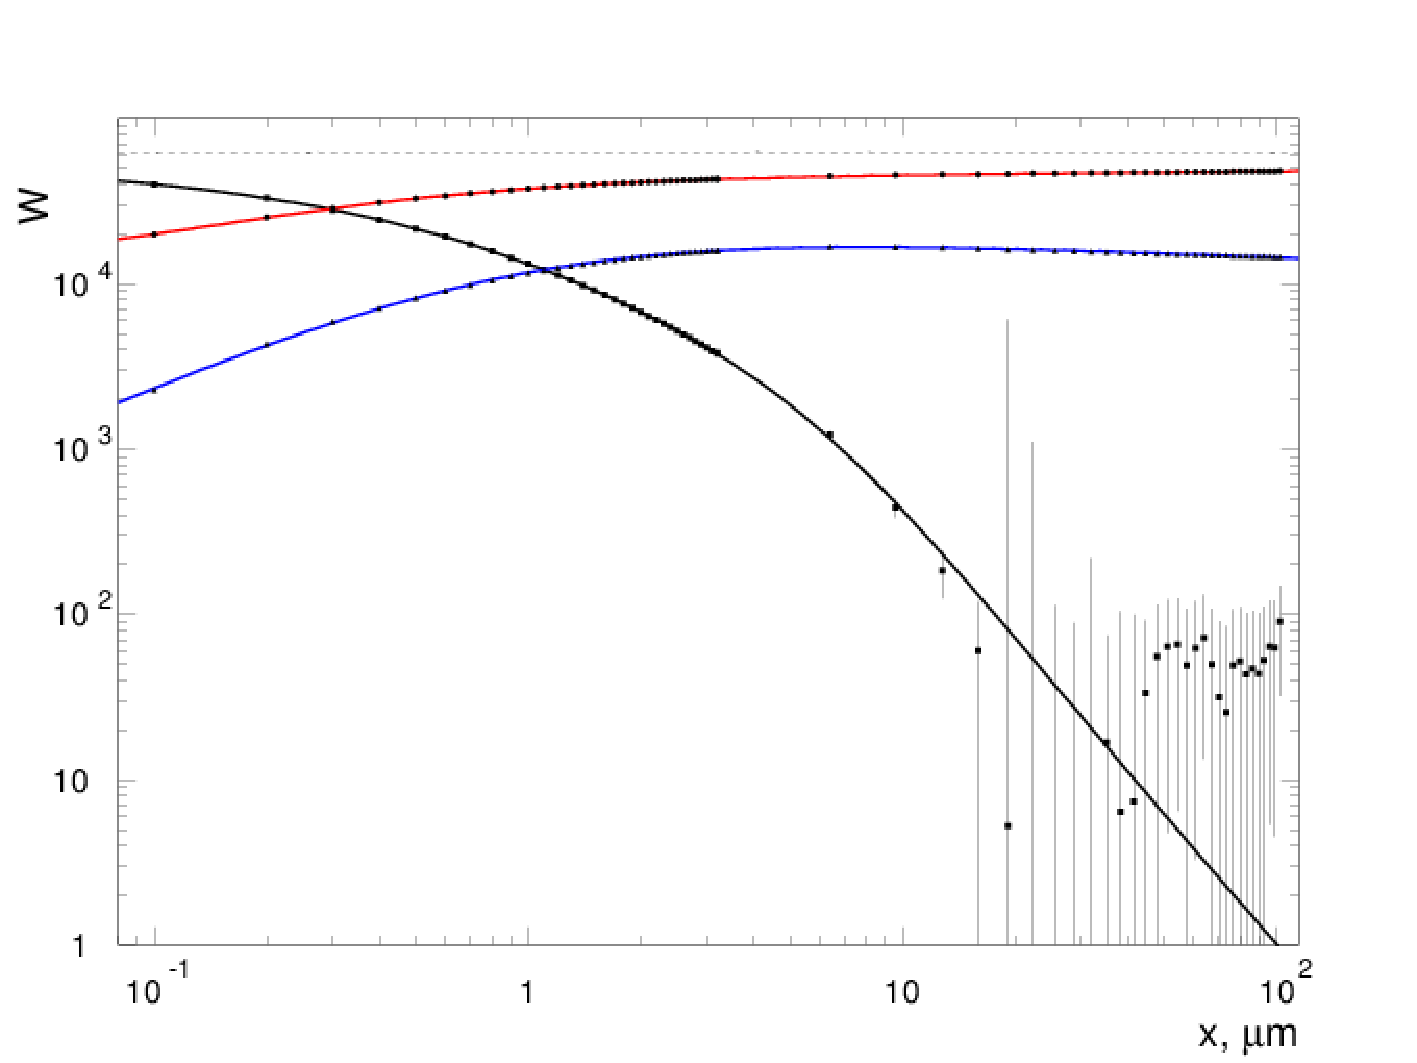
\includegraphics[width=0.99\linewidth]{images/pars135}
  }
  \caption{Изменение интегралов трёх гауссовых кривых с увеличением толщины пройденного слоя материала мишени.}
  \label{fig:Par1theta}
\end{figure}

	На Рис. ~\ref{fig:DispTheta} показан рост удвоенной дисперсии гауссианов при увеличении толщины пройденного слоя:

\begin{equation}
\label{MSApproximationD1}
\begin{aligned} 
D_1(x)=\frac{0.59\cdot 10^{-5}\cdot x}{1+\frac{0.029}{x}}, 
\end{aligned}
\end{equation}

\begin{equation}
\label{MSApproximationD2}
\begin{aligned} 
D_2(x)=D_1(x)+0.854\cdot 10^{-6}\cdot\left( 1+\left(\frac{x}{0.25} \right)^{1.108}\right)
\end{aligned}
\end{equation}

и

\begin{equation}
\label{MSApproximationD3}
\begin{aligned} 
D_3(x)=D_2(x)+0.8\cdot 10^{-5}\left( 1+\left(\frac{x}{1.28} \right)^{0.77}\right)\cdot\left( 1+\left(\frac{x}{132.37} \right)^{4.64}\right).
\end{aligned}
\end{equation}

\begin{figure}[ht]
  {
     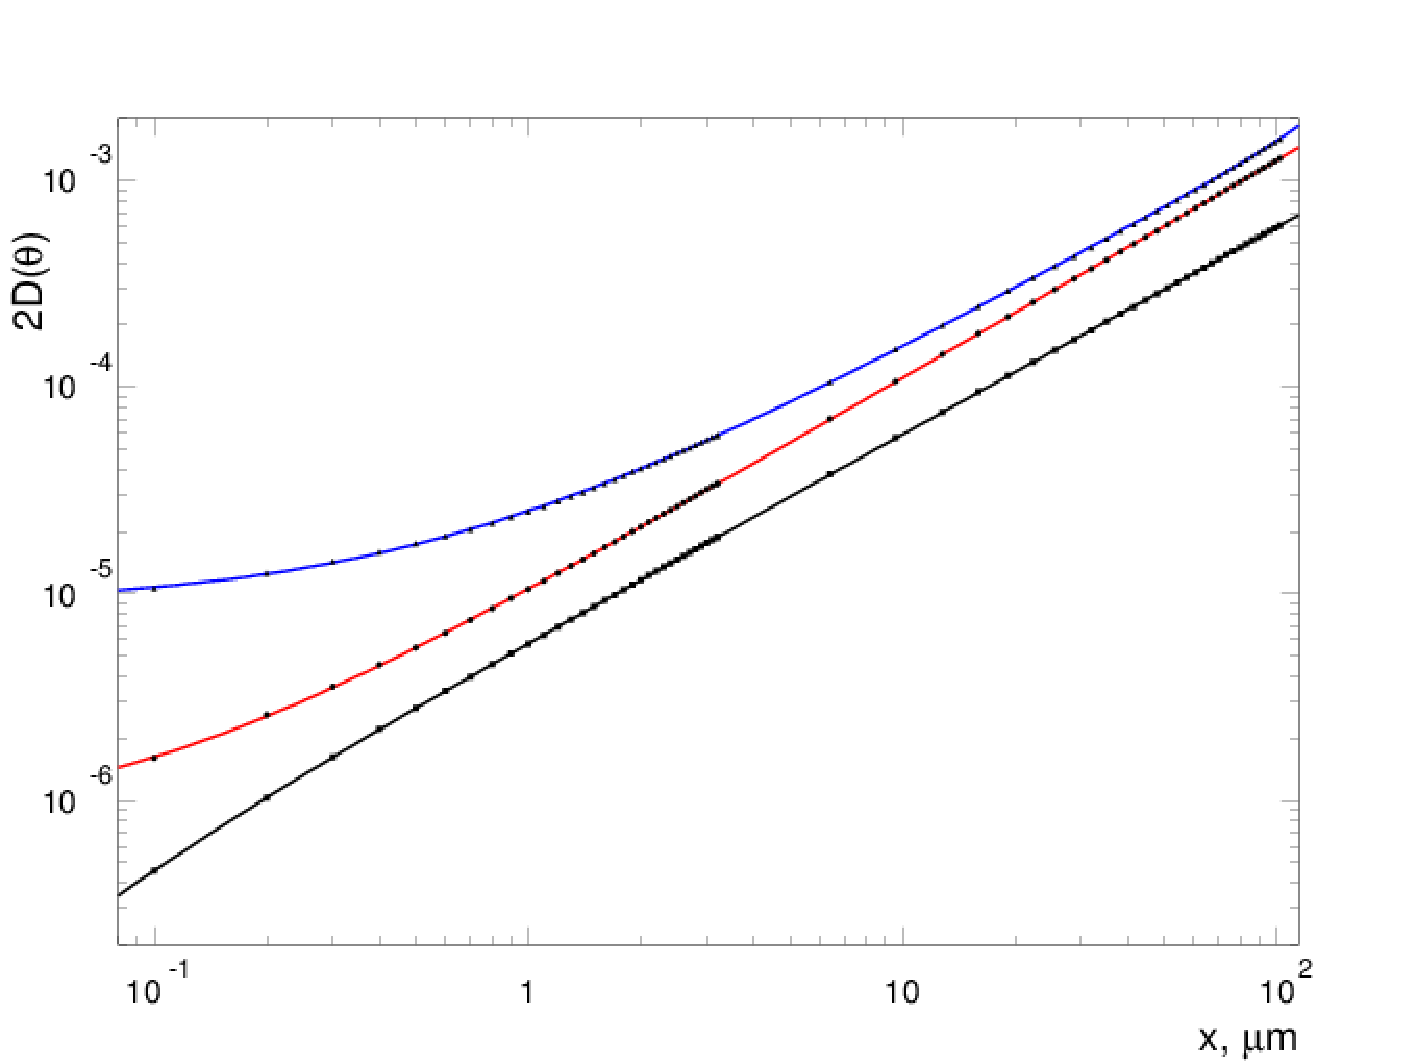
\includegraphics[width=0.99\linewidth]{images/pars246}
  }
  \caption{Изменение дисперсий трёх гауссовых кривых с увеличением толщины слоя.}
  \label{fig:DispTheta}
\end{figure}

	Заметим, что данный результат получен для случая, когда большие переданные импульсы в Резерфордовском рассеянии обрезаны и перенесены в дискретное моделирование.
	Осуществление передачи больших импульсов реализуется в дискретном процессе Резерфордовского рассеяния, в котором, в свою очередь, нет передачи малых импульсов, которая реализуется с помощью полученной аппроксимации и непрерывного процесса многократного рассеяния, включённого в моделирование.
  	Если пытаться учесть полное Резерфордовское рассеяние, вклад ``хвоста'' будет значительно больше, и он будет падать значительно медленнее, чем гауссово распределение.
  	По этой причине в реальных экспериментах обнаруживаются широкие ``крылья'', которые при использовании данной аппроксимации будут определяться дискретным рассеянием, учитывающим интерференцию резерфордовского и сильного рассеяния.
  
  	Также следует отметить, что данный результат был получен для многократного рассеяния в мишени из дейтерида титана дейтронов с кинетической энергией $T_{LS}$=10 МэВ.
  	Для использования полученной функции плотности вероятности углового распределения многократного рассеяния при других энергиях налетающих дейтронов, а также для углового распределения многократного рассеяния ионов титана в мишени из дейтерида титана, необходимо предложить некий метод пересчёта, скейлинг, позволяющий экстраполировать её область применимости с $Z=1$, $A=2$ и $T_{LS}$=10 МэВ на произвольные $T_{LS}$ и ионов титана.
  
\subsection{Пересчёт полученной аппроксимации углового распределения многократного рассеяния для произвольной кинетической энергии налетающей частицы и ионов титана.}
\label{subValMS2}

	Как известно, обычно для описания углового распределения многократного рассеяния используют одно распределение Гаусса, которое соответствует основному гауссиану в  (\ref{MSApproximationFunction}),т. е. вклады ``носа'' и ``хвоста'' в угловое распределение многократного рассеяния обычно не учитываются.
	С помощью аппроксимации экспериментальных данных получено [\underline{Ссылка на PDG!}] выражение для полуширины на полувысоте такого Гауссова распределения для широкого диапазона налетающих частиц и материалов:
\begin{equation}
  \label{Theta0}
  \theta_0=\frac{13.6 \cdot z \cdot \sqrt{\frac{x\cdot \rho}{X_0}}}{\beta_{LS}\cdot p_{LS}}\cdot\left[ 1+0.038\cdot\ln\left(\frac{x\cdot \rho}{X_0}\right)\right],
\end{equation}	

	При учёте $\beta_{LS}=\frac{p_{LS}}{E_{LS}}$ формула (\ref{Theta0}) принимает вид:
\begin{equation}
  \label{CheckTheta0Coefficient}
  \theta_0=13.6 \cdot z \cdot \sqrt{\frac{x\cdot \rho}{X_0}} \cdot \frac{E_{LS}}{p^2_{LS}} \cdot\left[ 1+0.038\cdot\ln\left(\frac{x\cdot \rho}{X_0}\right)\right],
\end{equation}
	где $x$ измеряется в сантиметрах, $X_0$ измеряется в г/см$^2$, поэтому используется плотность $\rho_{TiD_2}=3.91$ г/см$^3$, а $z$, $E_{LS}$ и $p_{LS}$ -- заряд, энергия и импульс налетающей частицы в лабораторной системе, измеряемые в МэВ.
	Для налетающего дейтрона с массой покоя $m_D=1875.6$ МэВ и кинетической энергией $T_{LS}=10$ МэВ его импульс $p_{LS}=193.94$ МэВ и полная энергия $E_{LS}=1885.6$ МэВ.
	Радиационная длина $TiD_2$ вычисляется из соотношения:
\begin{equation}
  \label{RadLength}
  \frac{A_{TiD_2}}{X_{0_{TiD_2}}}=\frac{2 A_{D}}{X_{0_{D}}}+\frac{A_{Ti}}{X_{0_{Ti}}},
\end{equation}
	где $A_i$ -- масса молекулы/элемента молекулы в атомных единицах массы (а.е.м.), а $X_{0_i}$ -- радиационная длина.
  	Так как $A_{TiD_2}=51.89$, $A_{D}=2.01$ и $A_{Ti}=47.87$, а также $X_{0_{D}}=125.98$ г/см$^2$ и $X_{0_{Ti}}=16.16$ г/см$^2$ \cite{PDG}, то $X_{0_{TiD_2}}=17.33$ г/см$^2$, что эквивалентно $\frac{X_{0_{TiD_2}}}{\rho_{TiD_2}}=4.43$ см.
  
  	Из формулы (\ref{CheckTheta0Coefficient}) можно получить, что дисперсия соответствующего углового распределения равняется
\begin{equation}
  \label{Theta0Dispersion}
   D(x)=2 \cdot \theta^2_0(x)=2 \cdot 13.6^2 \cdot z \cdot \frac{x\cdot \rho}{X_0} \cdot \frac{E^2_{LS}}{p^4_{LS}} \cdot\left[ 1+0.038\cdot\ln\left(\frac{x\cdot \rho}{X_0}\right)\right]^2.
\end{equation}  
  
  	Можно заметить, что величина $0.038\cdot\ln\left(\frac{x\cdot \rho}{X_0}\right)$ мала по сравнению с 1 при $x$ вплоть до десятков мкм, поэтому при моделировании толстой мишени из дейтерида титана, в которой произошла гауссизация углового распределения многократного рассеяния (для этого требуется, чтобы каждая частица перерассеялась много раз), ей можно пренебречь.
  	При моделировании же тонкой мишени, где вклад этой величины был бы значителен, формулой  (\ref{CheckTheta0Coefficient}) пользоваться нельзя, т. к. гауссизации углового распределения многократного рассеяния в результате большого количества перерассеяний частиц ещё не произошло, и поэтому трудно говорить об угловом распределении многократного рассеяния при малых $x$.
  
  	Из выражения (\ref{Theta0Dispersion}) видно, что $D(x) \sim z \cdot x \cdot \frac{E^2_{LS}}{p^4_{LS}}$. Получающаяся зависимость $D(x)$ совпадает по форме с основным гауссианом (\ref{MSApproximationD3}), если в нём пренебречь малым добавочным слагаемым с коэффициентом $10^{-6}$.
  	Т. к. при аппроксимации рассматриваются $x \geq 1$ мкм, выражение в знаменателе (\ref{MSApproximationD3}) стремится к 1.
  	В связи с этим в качестве скейлиногового коэффициента для пересчёта для других $E_{LS}$ и $z$ было выбрано выражение $z \cdot \frac{E^2_{LS}}{p^4_{LS}}$.
  
  	Таким образом, в первом приближении, пересчёт аппроксимации функции плотности вероятности углового рапсределния многоратного расссеяния для налетающих частиц с другой $E_{LS}$ и другим $z$ проводился следующим образом.
  	Вклады каждого из гауссианов $W_1$-$W_3$ брались без изменений.
  	А для их дисперсий $D_1$-$D_3$ выполнялось следующее: каждая $D_i$ делилась на $\frac{E^2_{LS}}{p^4_{LS}}$ для налетающего дейтрона с энергией 10 МэВ (для дейтрона $z=1$), т. к. аппроксимация (\ref{MSApproximationFunction}) была получена для налетающих дейтронов с энергией 10 МэВ, и умножалась на $z \cdot \frac{E^2_{LS}}{p^4_{LS}}$ для налетающей частицы с $E_{LS}$ и $z$, для которой необходимо было пересчитать аппроксимацию функции плотноости вероятности углового рапределения многократного рассеяния:
  	
\begin{equation}
  \label{DispersionScaling}
   \tilde D_i(x)[E_{LS}, z]=\frac{D_i(x) \cdot p^{4}_{LS}[D, 10 MeV]}{E^{2}_{LS}[D, 10 MeV]} \cdot z \cdot \frac{E^{2}_{LS}}{p^{4}_{LS}}.
\end{equation}  

	Полученная таким образом аппроксимация функции плотности вероятности углового распределения многократного рассеяния, применимая и для ионов дейтерия, и для ионов титана, при произвольных энергиях, использовалась при моделировании ионного каскада в мишени из дейтерида титана для описания непрерывного процесса многократного рассеяния частиц в веществе мишени.

	При помощи описанного способа скейлинга были получены угловые распределения функции плотности вероятности углового распределения многократного рассеяния для движущихся в мишени из дейтерида титана ионов дейтерия и титана при 3 толщинах пройденной ими рассеивающей среды -- 0.1 $\mu$м, 1 $\mu$м и 2.5 $\mu$м.
	Они показаны на Рис. ~\ref{fig:MFthetaScalingDeuteron} и ~\ref{fig:MFthetaScalingTitan}.
	
	
\begin{figure}[ht]
{
   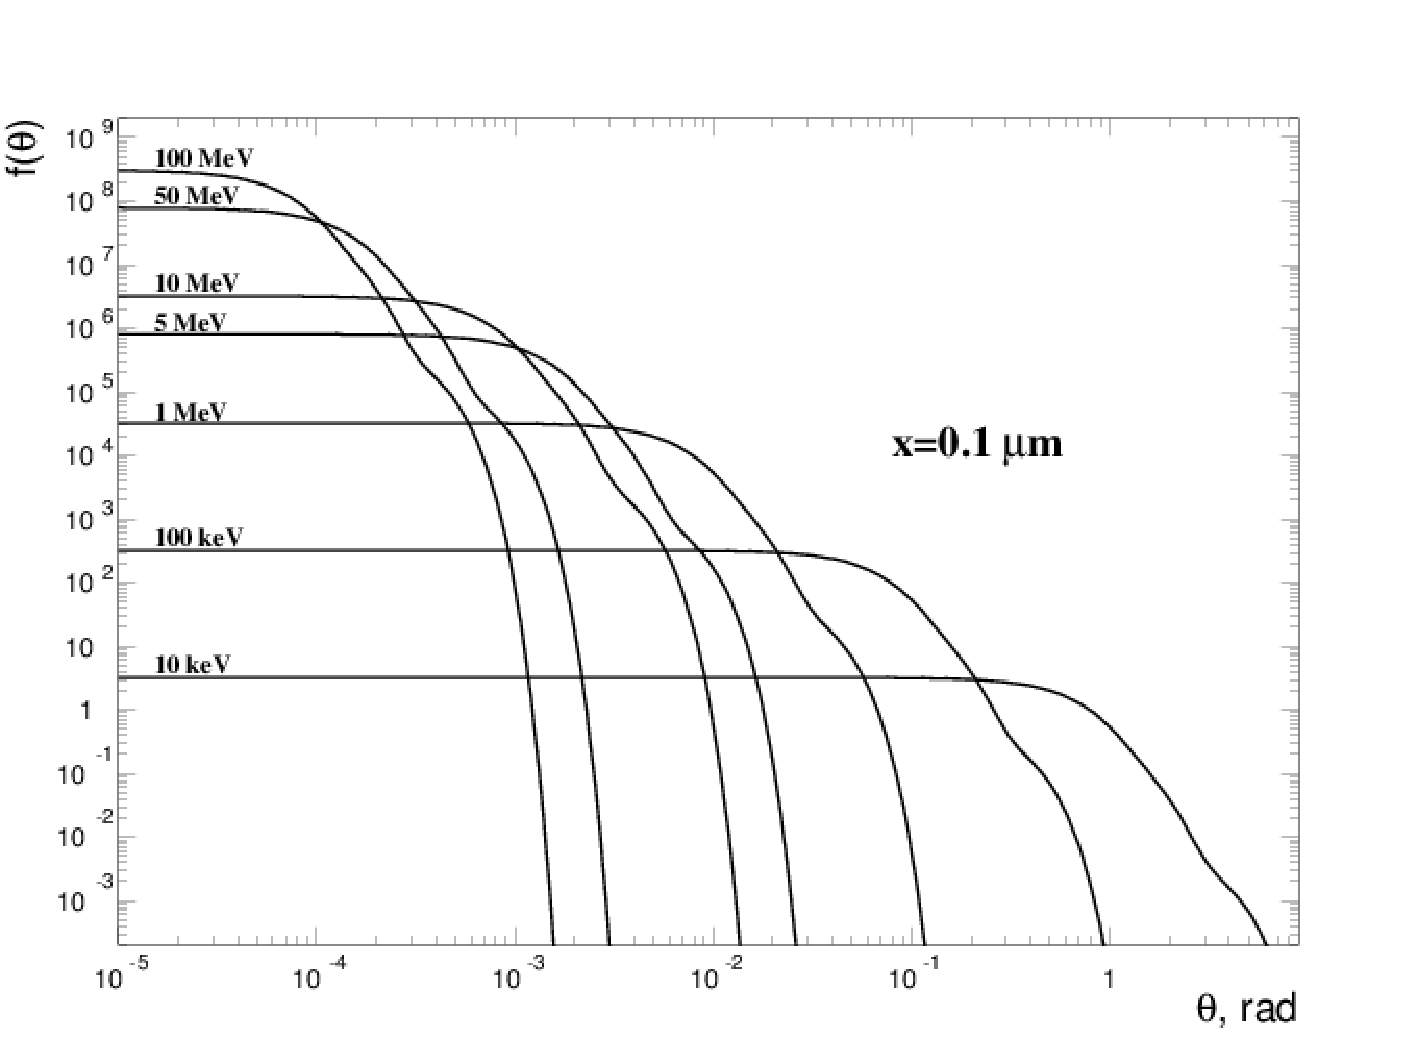
\includegraphics[width=0.32\linewidth]{images/funtheta_0_1mkm_deuteron.pdf}
   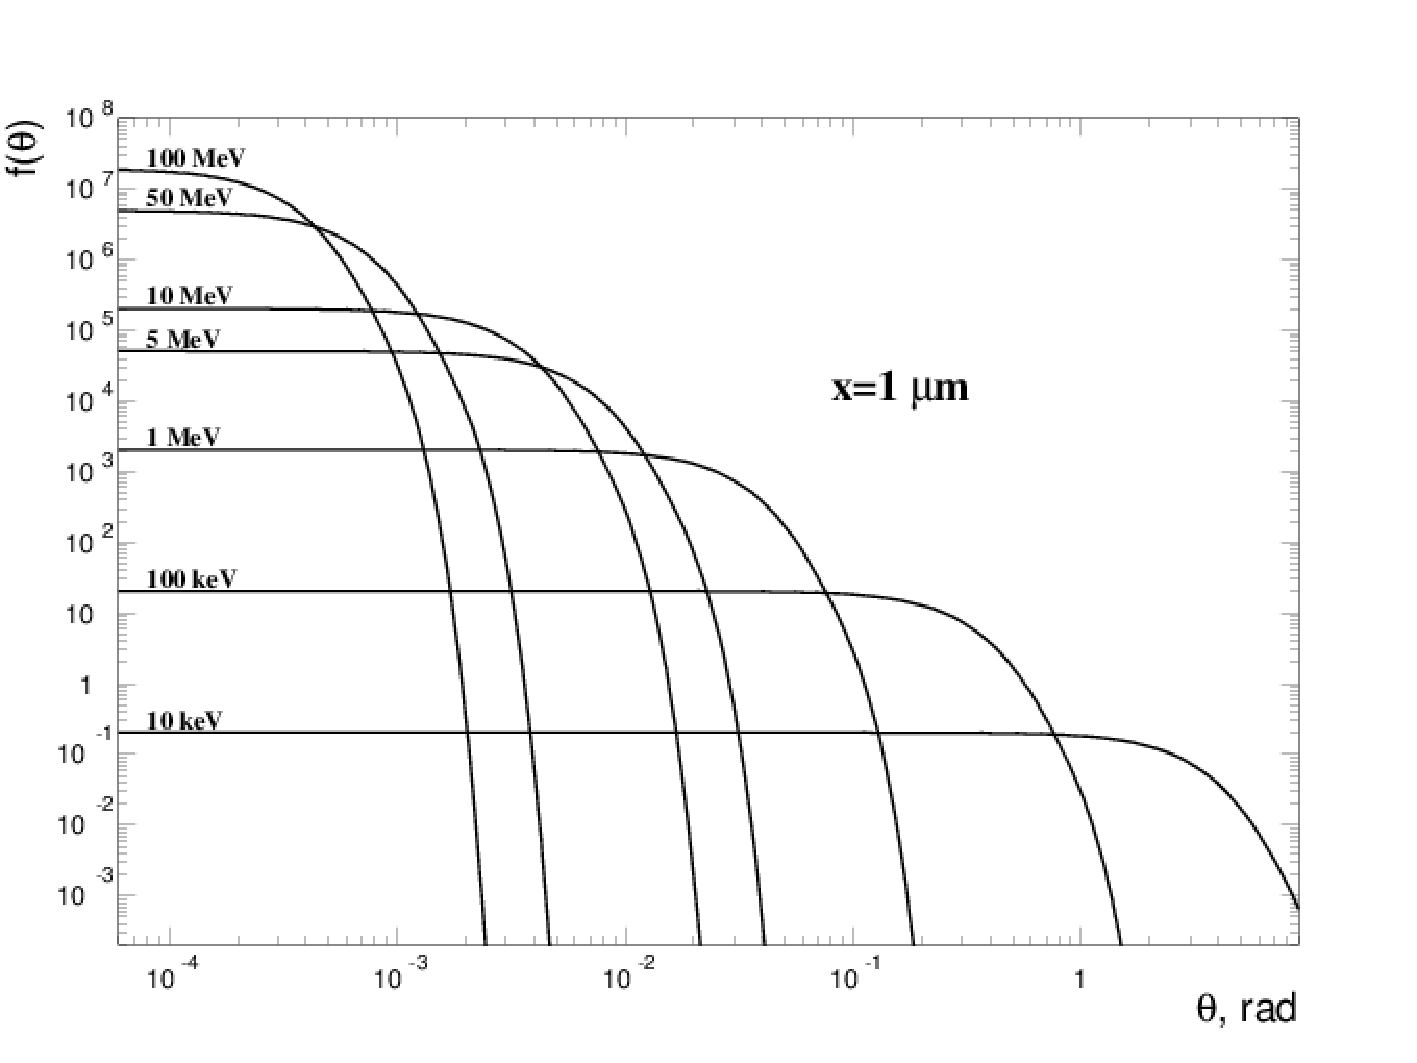
\includegraphics[width=0.32\linewidth]{images/funtheta_1mkm_deuteron.pdf}
   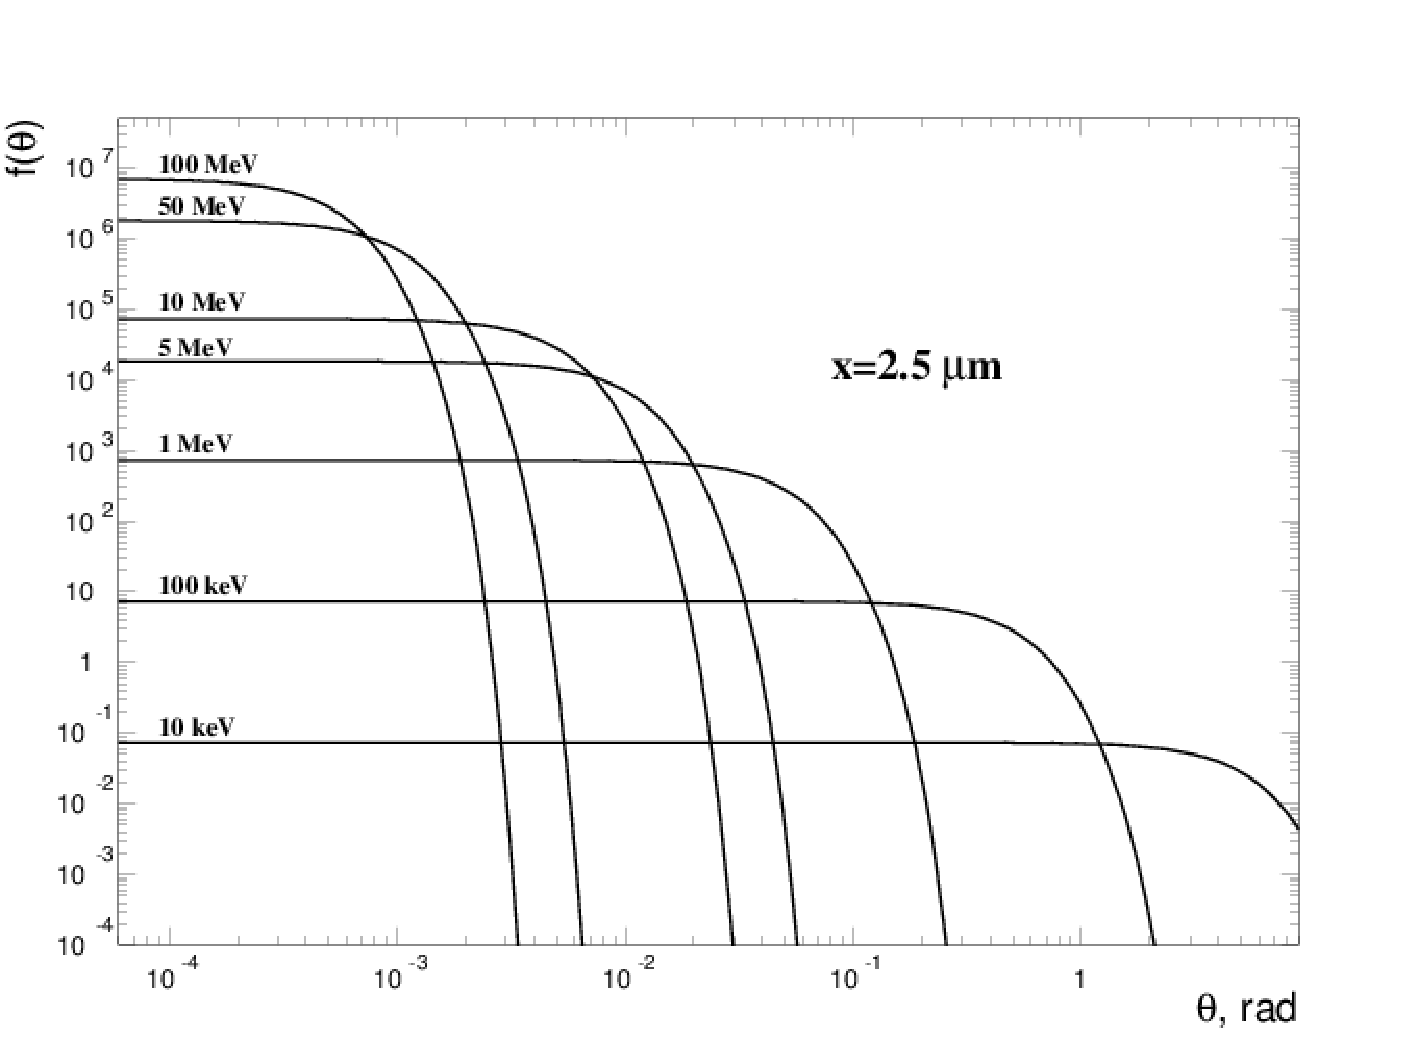
\includegraphics[width=0.32\linewidth]{images/funtheta_2_5mkm_deuteron.pdf}
}
\caption{Пересчёт (скейлинг) полученной для дейтерия с кинетической энергией 10 МэВ в дейтериде титана аппроксимации функции плотности вероятности углового распределения многократного рассеяния $f(\theta)$ для произвольных кинетических энергий налетающего иона дейтерия.
	Показаны зависимости при толщинах пройденной рассеивающей среды 0.1 $\mu$м, 1 $\mu$м и 2.5 $\mu$м.}
\label{fig:MFthetaScalingDeuteron}
\end{figure}

\begin{figure}[ht]
{
   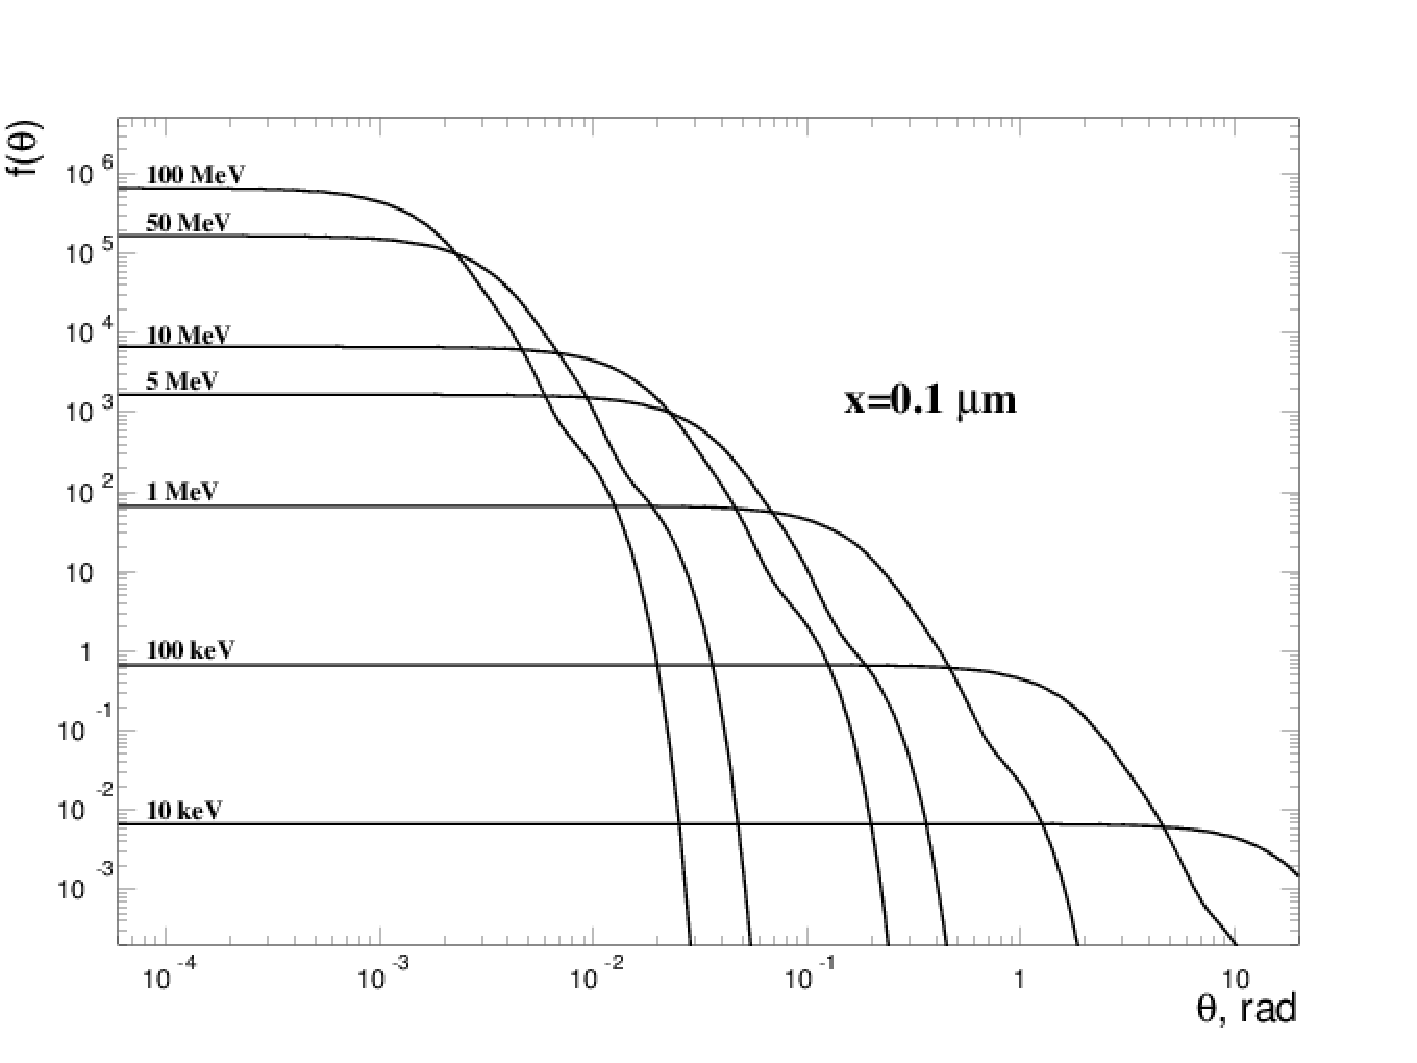
\includegraphics[width=0.32\linewidth]{images/funtheta_0_1mkm_ti.pdf}
   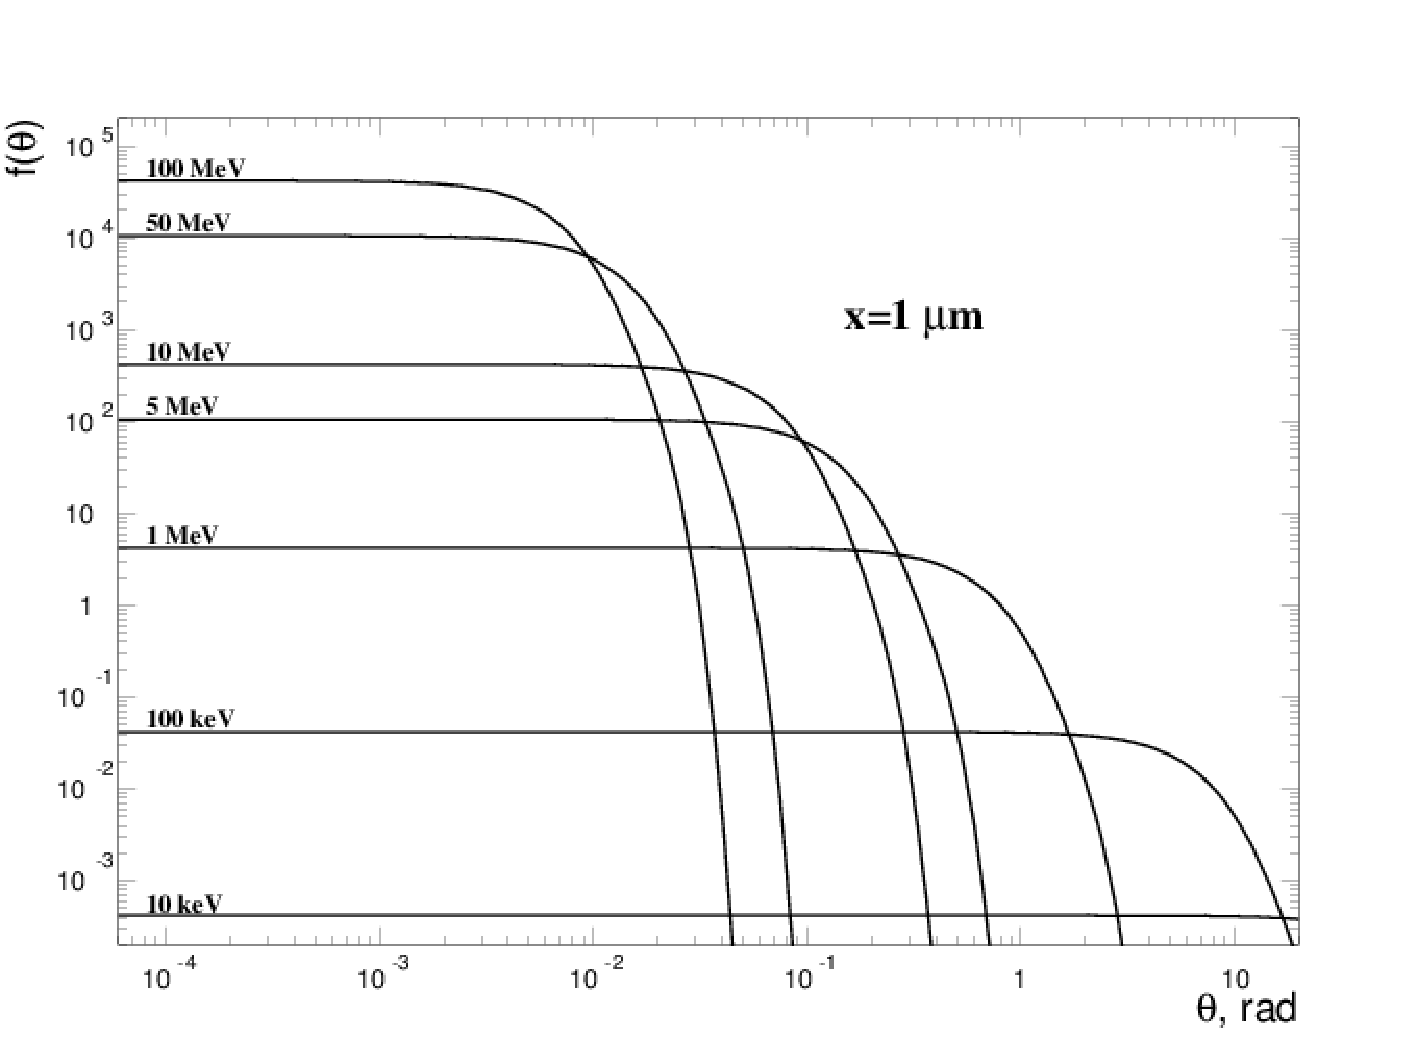
\includegraphics[width=0.32\linewidth]{images/funtheta_1mkm_ti.pdf}
   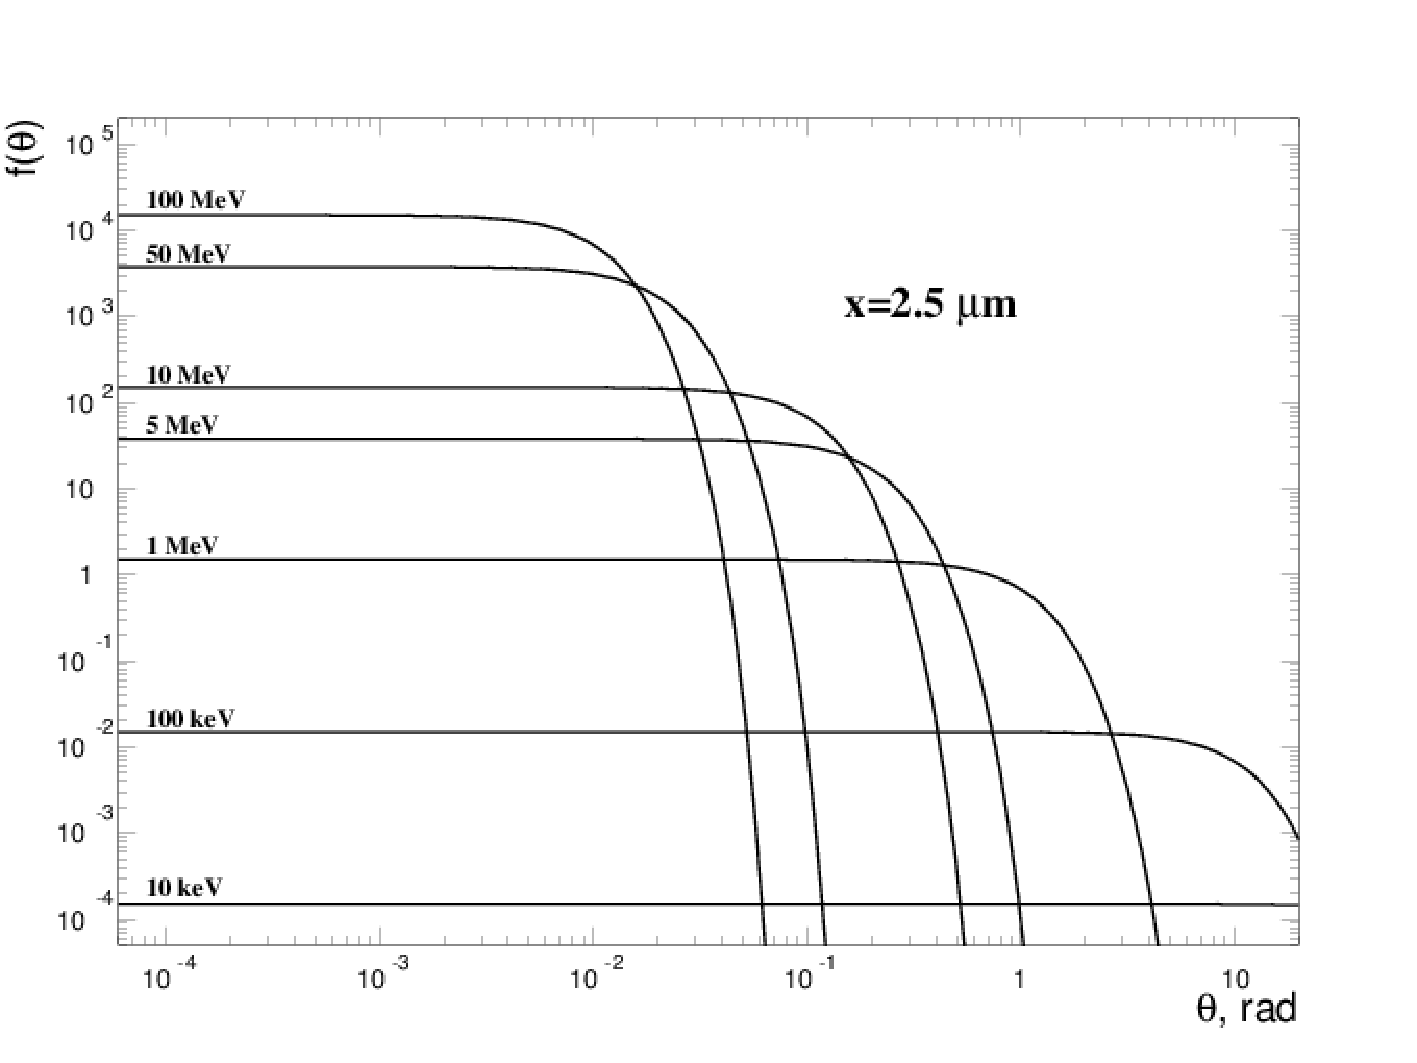
\includegraphics[width=0.32\linewidth]{images/funtheta_2_5mkm_ti.pdf}
}
\caption{Пересчёт (скейлинг) полученной для дейтерия с кинетической энергией 10 МэВ в дейтериде титана аппроксимации функции плотности вероятности углового распределения многократного рассеяния $f(\theta)$ для произвольных кинетических энергий налетающего иона титана.
	Показаны зависимости при толщинах пройденной рассеивающей среды 0.1 $\mu$м, 1 $\mu$м и 2.5 $\mu$м.}
\label{fig:MFthetaScalingTitan}
\end{figure}

	Также было необходимо проверить, правильно ли работает генерация случайного угла многократного рассеяния из данного распределения с помощью генератора псевдослучайных чисел в процессе моделирования.
	Для проверки бралась полученная аппроксимация (\ref{MSApproximationFunction}) углового распределения многократного рассеяния дейтронов с кинетической энергией 10 МэВ в мишени из дейтерида титана.
	
\subsection{Проверка правильности углового распределения, сгенерированного в параллельном коде.}
\label{subValMS3}

	При интегрировании плотности вероятности (\ref{MSApproximationFunction}) надо вычислять не интеграл $\int\limits_{0}^{\tilde \theta} f(\theta) \cdot d\theta$, а интеграл $\int\limits_{0}^{\tilde \theta} f(\theta) \cdot \theta d\theta$, поскольку $\theta$ имеет смысл полярного угла, а значит интегрировать надо по элементу угловой площади $\theta \cdot d \theta$.
	
	В результате интегрирования (\ref{MSApproximationFunction}) получается выражение:
	
\begin{equation}
\label{MSApproximationFunctionIntegral}
\begin{aligned} 
  \int \limits_0^{\infty} \theta \cdot f(\theta) \cdot d\theta=\sum_{i=1}^{3} \frac{W_i}{D_i} \int \limits_0^{\infty} e^{-\frac{\theta^2}{D_i}} \cdot 2 \theta\cdot d\theta = \sum_{i=1}^{3} W_i.
\end{aligned}
\end{equation}

  	Розыгрыш угла начинается с того, что с помощью случайного числа выбирается одно из гауссовых распределений ($W_i,D_i$), относительные вероятности которых рассчитываются по формуле $\frac{W_i}{\sum_{i=1}^{3}W_i}$.
  
  	Угол для выбранного Гауссова распределения разыгрывается как $\theta=\sqrt{-2D_i\cdot\ln{R}}$, где $R$ -- случайное число от 0 до 1, то есть используется функция, обратная к гауссовой экспоненте.
  
 	Таким образом, в полной версии программного кода, использующей эффективное распараллеливание по потокам OpenMP и максимально возможную векторизацию, было запущено $N_P=100$ миллионов дейтронов с начальной кинетической энергией 10 МэВ.
 	Их случайные угла многократного рассеяния записывались в гистограмму из $N_{bin}=100$ бинов с логарифмическим шагом от $\theta_{min}=10^{-4}$ рад до $\theta_{max}=0.05$ рад.
 	Границы бинов определялись как $\theta_i=e^{\ln{\theta_{min}+i \cdot \Delta \ln{\theta}}}$, где логарифмический шаг по оси $\theta$ есть $\Delta \ln{\theta}=\frac{\ln{\theta_{max}}-\ln{\theta_{min}}}{N_{bin}-1}$.
 	В итоге получались $N_{bin}$ величин $\Delta N_i$, соответствующих числу событий в каждом из $N_{bin}$ логарифмических бинов.
 	Эти величины $\Delta N_i$ для нормировки (функция плотности вероятности (\ref{MSApproximationFunction}) нормирована на 1 частицу) делились на полное число частиц, равное $N_P$, и на величину $\theta_i^2 \cdot \Delta \ln{\theta}=\theta_i \cdot \Delta \theta_i$, соответствующую бесконечно малому элементу угловой площади, где величина $\theta^{mid}_i$ бралась в среднегеометрической середине бина, равной $\theta^{mid}_i=\sqrt{ \theta_i \cdot \theta_{i+1}}$ при $i$, изменяющемся от 0 до $N_{bin}-1$.
 	Получалась величина $f(\theta_i)=\frac{1}{N_P} \cdot \frac{\Delta N_i}{\Delta\ln{\theta} \cdot \theta^2_i}=\frac{1}{N_P} \cdot \frac{\Delta N_i}{\theta_i \cdot \Delta \theta_i}$.
  
 	В итоге были выбраны 6 значений толщины пройденного потоком из $N_P$ частиц слоя вещества, и для каждого из них построены гистограммы отношения полученной в ходе моделирования $f(\theta_i)$ к точно вычисленному по найденной аппроксимации (\ref{MSApproximationFunction}) в среднегеометрической середине логарифмического бина $\theta^{mid}_i$ значению функции плотности верятности углового распределения многократного рассеяния.
 	Результат изображён на Рис. ~\ref{fig:MSRatioHistogramWithoutCorrection}.
 	
\begin{figure}[ht]
{
   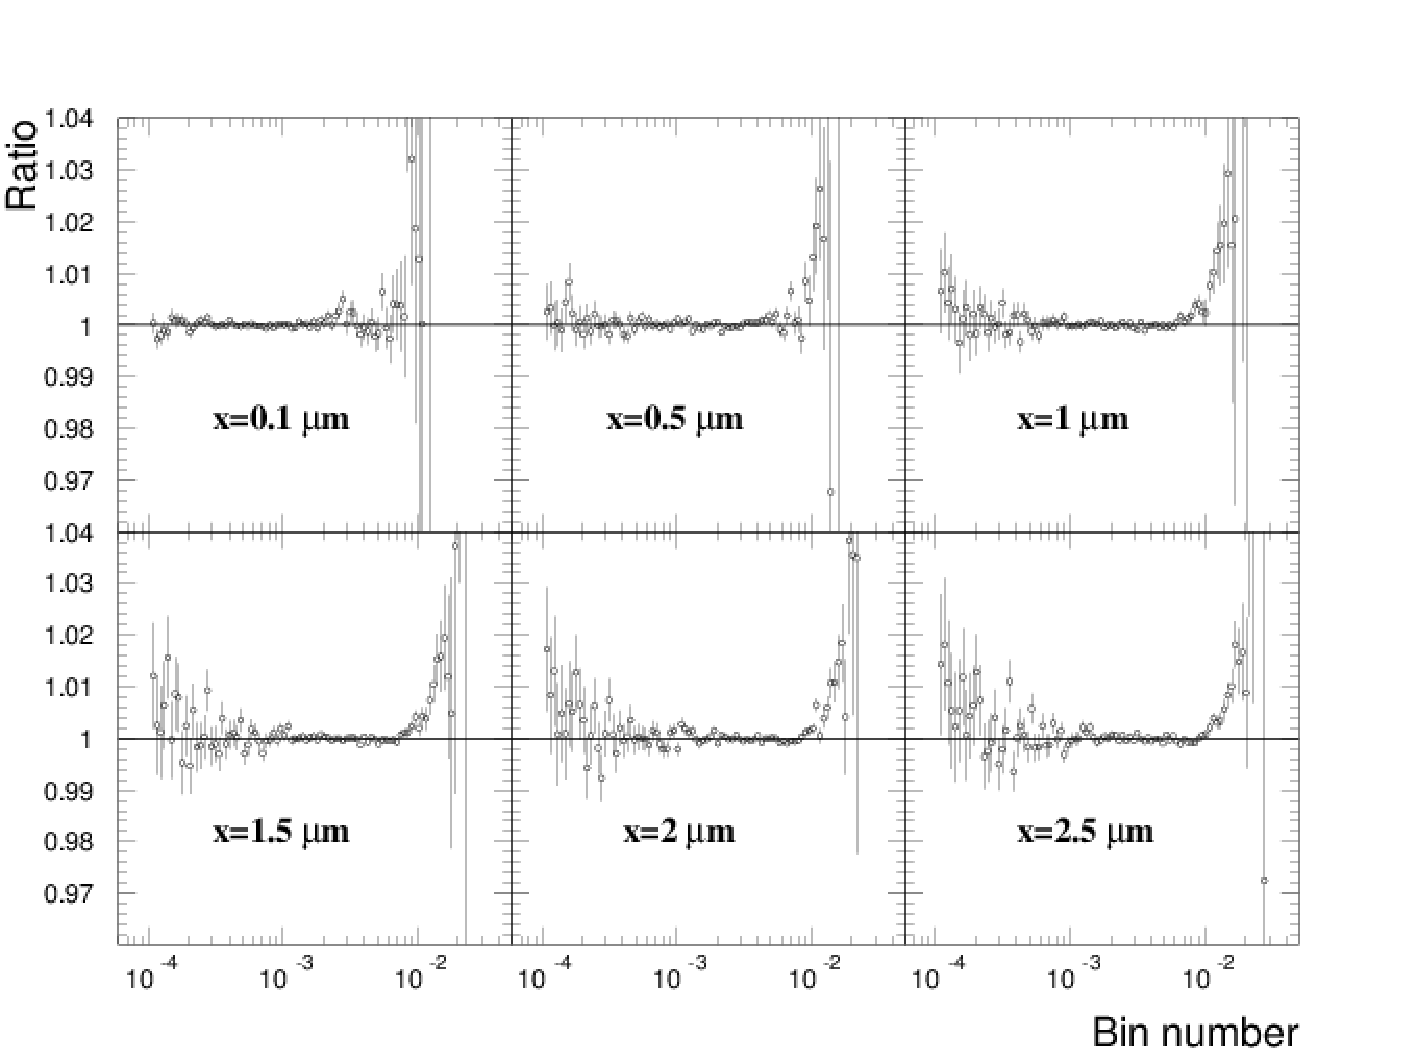
\includegraphics[width=0.99\linewidth]{images/ratioms_without_correction.pdf}
}
\caption{Отношение полученной в ходе моделирования $f(\theta_i)$ к точно вычисленному по найденной аппроксимации (\ref{MSApproximationFunction}) в среднегеометрической середине логарифмического бина $\theta^{mid}_i$ значению функции плотности верятности углового распределения многократного рассеяния.}
\label{fig:MSRatioHistogramWithoutCorrection}
\end{figure}

	Из Рис. ~\ref{fig:MSRatioHistogramWithoutCorrection} видно, что в целом отношение близко к 1 с очень хорошей точностью, но при приближении к правой границе гистограммы наблюдается его явный рост.
	Было выяснено, что этот рост связан с тем, что логарифмические бины гистограммы растут слева направо, у правой границы гистограммы их размер сильно возрастает.
	В то же время функция (в (\ref{MSApproximationFunction}) входят 3 гауссоиды, но без ограничения общности для простоты можно рассматривать 1 распределение Гаусса) распределения Гаусса является сильно падающей.
	Поэтому то, какому значению $\theta$ в каждом бине соответсвует полученное в ходе моделирования $f(\theta_i)$, нужно находить интегрированием, в то время как у нас берётся среднегеометрическая середина бина $\theta^{mid}_i$.
	Наблюдающийся рост отношения свидетельствует о том, что в правых бинах гистограммы ``среднее'' рассчитанное путём интегрирования значение $\theta$ лежит правее $\theta^{mid}_i$, а мы как бы занижаем это значение $\theta$, тем самым завышая значение $f(\theta_i)$, чем и объясняется загиб вверх отношения у правой границы гистограммы. Подробные выкладки приводятся ниже.
  
\subsection{Коррекция углового распределения, сгенерированного в параллельном коде, в связи с логарифмической шкалой гистограммы и сильно падающей функцией распределения Гаусса.}
\label{subValMS4}

	Если проинтегрировать функцию распределения Гаусса $F(\theta)=C \cdot \frac{2}{D} \cdot e^{-\frac{\theta^2}{D}}$, где нормировочный коэффициент $C$ мы в дальнейшем опустим, по угловой площади $\theta \cdot d\theta$ в пределах заданного бина (здесь рассматривается линейный масштаб, но аналогичные выкладки можно провести и в логарифмическом масштабе, проводя интегрирование по оси $\ln{\theta}$, которая в этом случае будет линейна), чтобы получить среднее значение функции $F(\theta)$ в этом бине, получится
\begin{equation}
\label{MSIntegralExp}
\begin{aligned} 
  \langle f \rangle = \frac{1}{2\Delta} \cdot \int \limits_{\theta_{mid} - \Delta}^{\theta_{mid} + \Delta} \theta \cdot F(\theta) \cdot d \theta =
  \frac{e^{-\frac{\left( \theta_{mid} - \Delta \right)^2}{D}} - e^{-\frac{\left( \theta_{mid} + \Delta \right)^2}{D}}}{2\Delta} = \\
  e^{-\frac{\theta^2_{mid} + \Delta^2}{D}} \cdot \frac{ e^{\frac{2 \cdot \theta_{mid} \cdot \Delta}{D}} - e^{-\frac{2 \cdot \theta_{mid} \cdot \Delta}{D}} }{2\Delta},
\end{aligned}
\end{equation}
	где $\theta$ -- полуширина бина, а $\theta_{mid}$ -- его середина.

	Если воспользоваться разложением экспоненты в ряд по малому параметру $\frac{2 \cdot \theta_{mid} \cdot \Delta}{D}$, можно получить, что
\begin{equation}
\label{MSIntegralExpand}
\begin{aligned} 
  \frac{ e^{\frac{2 \cdot \theta_{mid} \cdot \Delta}{D}} - e^{-\frac{2 \cdot \theta_{mid} \cdot \Delta}{D}} }{2\Delta} =
  \frac{2 \cdot \theta_{mid}}{D}.
\end{aligned}
\end{equation}
	Т. к. $\frac{2 \cdot \theta_{mid} \cdot \Delta}{D}$ -- малый параметр, то раскладываем экспоненту только до 1-го порядка малости, чётные степени сокращаются, а нечётные высших порядков не вносят вклада из-за малости параметра.

	В итоге выражение (\ref{MSIntegralExp}) принимает вид
\begin{equation}
\label{MSIntegralFin}
\begin{aligned} 
  \langle f \rangle = \frac{2}{D} \cdot e^{-\frac{\theta^2_{mid}}{D}} \cdot \theta_{mid} \cdot e^{-\frac{\Delta^2}{D}} .
\end{aligned}
\end{equation}

	В нём первое слагаемое $\frac{2}{D} \cdot e^{-\frac{\theta^2_{mid}}{D}}$ с точностью до нормировочного коэффициента соответствует точному значение функции аппроксимации углового распределения многократного рассеяния, рассчитанному в середине бина $\theta_{mid}$, а множитель $\theta_{mid} \cdot e^{-\frac{\Delta^2}{D}}$ как раз и отвечает за загиб вверх в правой части гистограммы на Рис. ~\ref{fig:MSRatioHistogramWithoutCorrection}.
	
	Поэтому, если скорректировать полученные в результате моделирования значения $f(\theta_i)$, поделив их на $\theta_{mid} \cdot e^{-\frac{\Delta^2}{D}}$, рост в правой части гистограммы на Рис. ~\ref{fig:MSRatioHistogramWithoutCorrection} должен исчезнуть.
	Результат показан на Рис. ~\ref{fig:MSRatioHistogramWithCorrection}.
	Как видно, аномальный рост исчез, и отношение в пределах погрешности равно 1.
	
\begin{figure}[ht]
{
   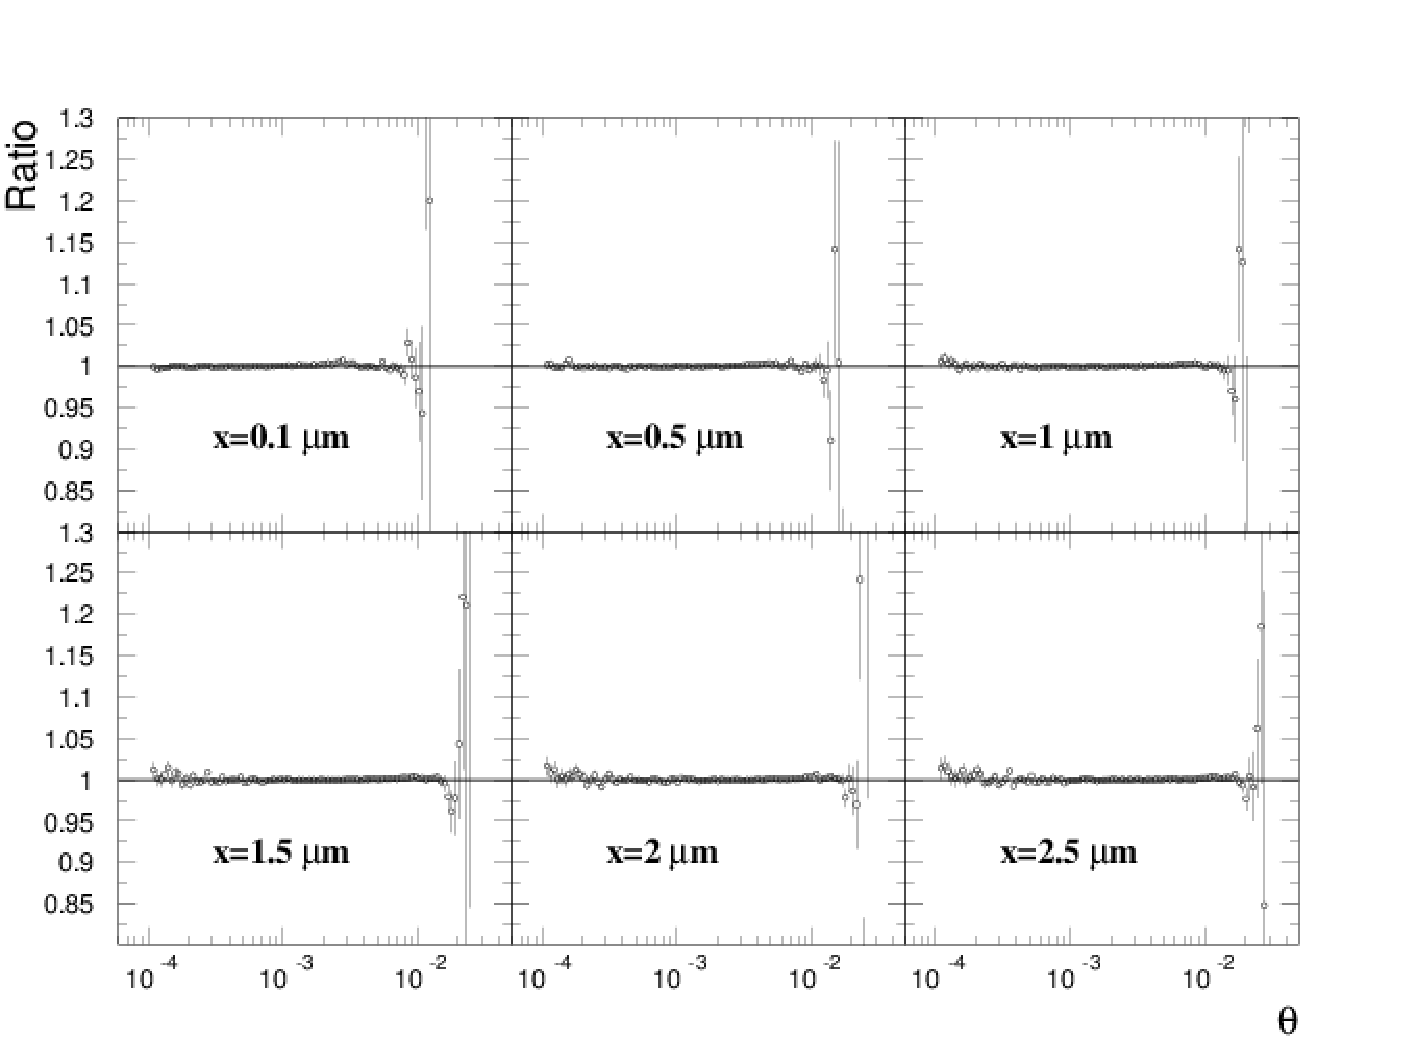
\includegraphics[width=0.99\linewidth]{images/ratioms_with_correction.pdf}
}
\caption{Отношение полученной в ходе моделирования $f(\theta_i)$ \underline{после коррекции} к точно вычисленному по найденной аппроксимации (\ref{MSApproximationFunction}) в среднегеометрической середине логарифмического бина $\theta^{mid}_i$ значению функции плотности верятности углового распределения многократного рассеяния.}
\label{fig:MSRatioHistogramWithCorrection}
\end{figure}

	Как видно из (\ref{MSIntegralFin}), данная коррекция необходима и при линейное шкале, когда $\Delta=const$, но при логарифмической шкале $\Delta$ сильно растёт справа налево оси $x$, и коэффициент корректировки гораздо больше.
	Независимо от шкалы присутствует коэффициент $\theta_{mid}$, который необходимо корректировать.

	Таким образом, было показано, что многократное рассеяние можно успешно моделировать в параллельном и векторизованном программном коде при помощи полученной аппроксимации его углового распределения (\ref{MSApproximationFunction}).
	
	
\clearpage{}
\section{Валидация углового распределения неупругой D-D реакции.}
\label{ValInelasticDD}

	Для моделирования ионного каскада в мишени из дейтерида титана, вызванного облучением мишени потоком дейтронов, необходимо знать интегральное сечение и угловое распределение неупругой D-D реакции. 
	
	Экспериментальные данные интегральных сечений обоих каналов (p+t и n+$^3_2$He) брались из базы данных ENDF-6 и аппроксимировались дробно-рациональными функциями.
	В результате чего были получены функции зависимости интегрального сечения каждого из каналов неупругой D-D реакции от кинетической энергии налетающего дейтрона в системе центра масс $T_{CM}$, равной для случая рассеяния одинаковых частиц половине кинетической энергии налетающей частицы в лабораторной системе $T_{LS}$:
	
\begin{equation}
\label{InelasticDDNHe3ChannelIntegralCrossSection}
\begin{aligned} 
  \sigma^{n+^3_2He}(T_{CM}) = \frac{0.21}{\left( 1 + \left(\frac{2.52\cdot 10^{-2}}{T_{CM}} \right)^{1.5} \right) \cdot \left( 1 + \left( \frac{4.7\cdot 10^{-3}}{T_{CM}} \right)^{4.5} \right) \cdot \left( 1+0.23 \cdot T_{CM} \right) } \cdot g
\end{aligned}
\end{equation}

и

\begin{equation}
\label{InelasticDDPTChannelIntegralCrossSection}
\begin{aligned} 
  \sigma^{p+t}(T_{CM}) = \frac{0.176}{\left( 1 + \left(\frac{2\cdot 10^{-2}}{T_{CM}} \right)^{1.7} \right) \cdot \left( 1.0 + \left( \frac{4.3\cdot 10^{-3}}{T_{CM}} \right)^{4.4} \right) \cdot \left( 1+\left( 0.17 \cdot T_{CM} \right)^{0.85} \right) } \cdot g,
\end{aligned}
\end{equation}
	
	где фактор Гамова есть $g=e^{-\frac{1}{2}\sqrt{\frac{Eg}{T_{CM}}}}$, а $E_g$ -- энергия Гамова, равная для D-D рассеяния 0.986 МэВ.
	На Рис. ~\ref{fig:InelasticDDIntegralCrossSections} изображены выражения (\ref{InelasticDDNHe3ChannelIntegralCrossSection}) и (\ref{InelasticDDPTChannelIntegralCrossSection}), делённые на фактор Гамова.
	Они определяют величину сечений соответствующих каналов реакции в барнах.
	
\begin{figure}[ht]
  {
     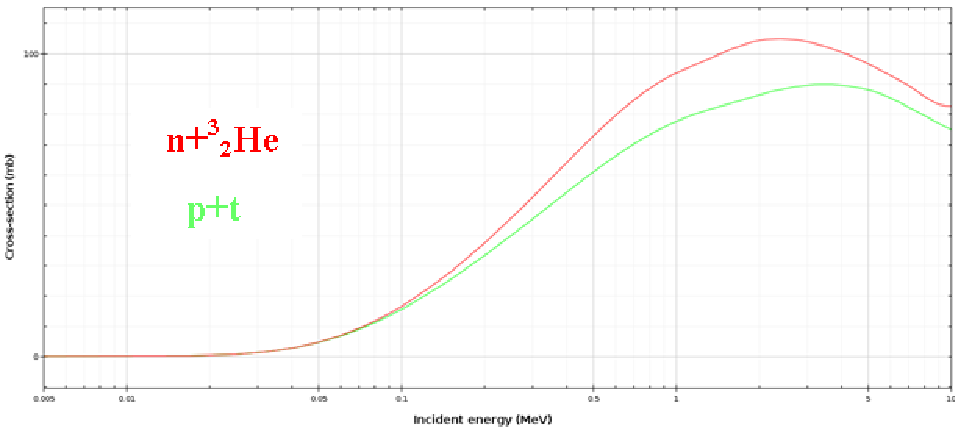
\includegraphics[width=0.99\linewidth]{images/DDInelasticIntegralCrossSections.pdf}
  }
  \caption{Зависимость интегральных сечений каналов неупругой D-D реакции от кинетической энергии в системе центра масс $T_{CM}$.}
  \label{fig:InelasticDDIntegralCrossSections}
\end{figure}	
	
	
	Угловые распределения неупругой D-D реакции брались из базы данных TPT2 в виде нормированных частичных сумм от -1 до 1 по $\cos{ \left( \theta_{CM} \right) }$.
	В базе данных ТРТ2 записаны нормированные частичные суммы для каждой из 127 значений кинетической энергии от $10^{-4}$ МэВ до 10 МэВ с линейным шагом.
	Эти 127 наборов из энергий и частичных сумм читались из базы данных ТРТ2 и с помощью линейной интерполяции из них получалась более подробная база данных частичных сумм для 512 значений кинетической энергии налетающего дейтрона с линейным шагом в том же диапазоне.
	Из них с помощью случайных чисел и квадратичной интерполяции получались значения $\cos{ \left( \theta_{CM} \right) }$ в ходе моделирования.
	Квадратичная интерполяция использовалась для более точного описания углового распределения.
	Ведь если использовать линейную интерполяцию, это приведёт к тому, что описание углового распределения, сгенерированное с помощью случайных чисел, будет ступенчатым, а при использовании квадратичной интерполяции сгенерированное угловое распределение будет сплайном, проходящим по точкам, соответствующим значениям частичных сумм.
	
	Нужно было проверить правильность сгенерированного в ходе моделирования с помощью разрабатываемого параллельного программного кода TPT3 углового распределения неупругой реакции D+D.
	Т. к. нормализованные частичные суммы, записанные в базу данных ТРТ2, получены интегрированием полиномов Лежандра, коэффициенты разложения углового распределения неупругой D-D реакции по которым заданы в базе ENDF-6, из-за сложности полиномов Лежандра, очевидно, не представляется возможным получить аналитическую функцию, с помощью которой можно было бы провести нужное сравнение.
	Поэтому было проведено моделирование неупругой D-D реакции в тонкой мишени с помощью Geant.
	В ходе моделирования запускалось 2 миллиарда дейтронов и с помощью программного пакета ROOT заполнялись гистограммы нормированного углового распределения продуктов реакции при различных кинетических энергиях налетающих дейтронов.
	Данные гистограммы нормированного дифференциального сечения сравнивались с полученными при моделировании разрабатываемым параллельным программным кодом TPT3 при нескольких значениях кинетической энергии налетающего дейтрона в лабораторной системе, и при всех этих значениях кинетической энергии получилось отличное совпадение с расхождением не более 1 процента результатов моделирования Geant4 и разрабатываемым программным кодом, работающим и на CPU, и на GPU.
	Например, при кинетической энергии налетающего дейтрона, равной 2 МэВ, соотношение результатов моделирования изображено на  Рис. ~\ref{fig:ValidationThermonuclear2mev2billionParticles}.
	
\begin{figure}[ht]
  {
     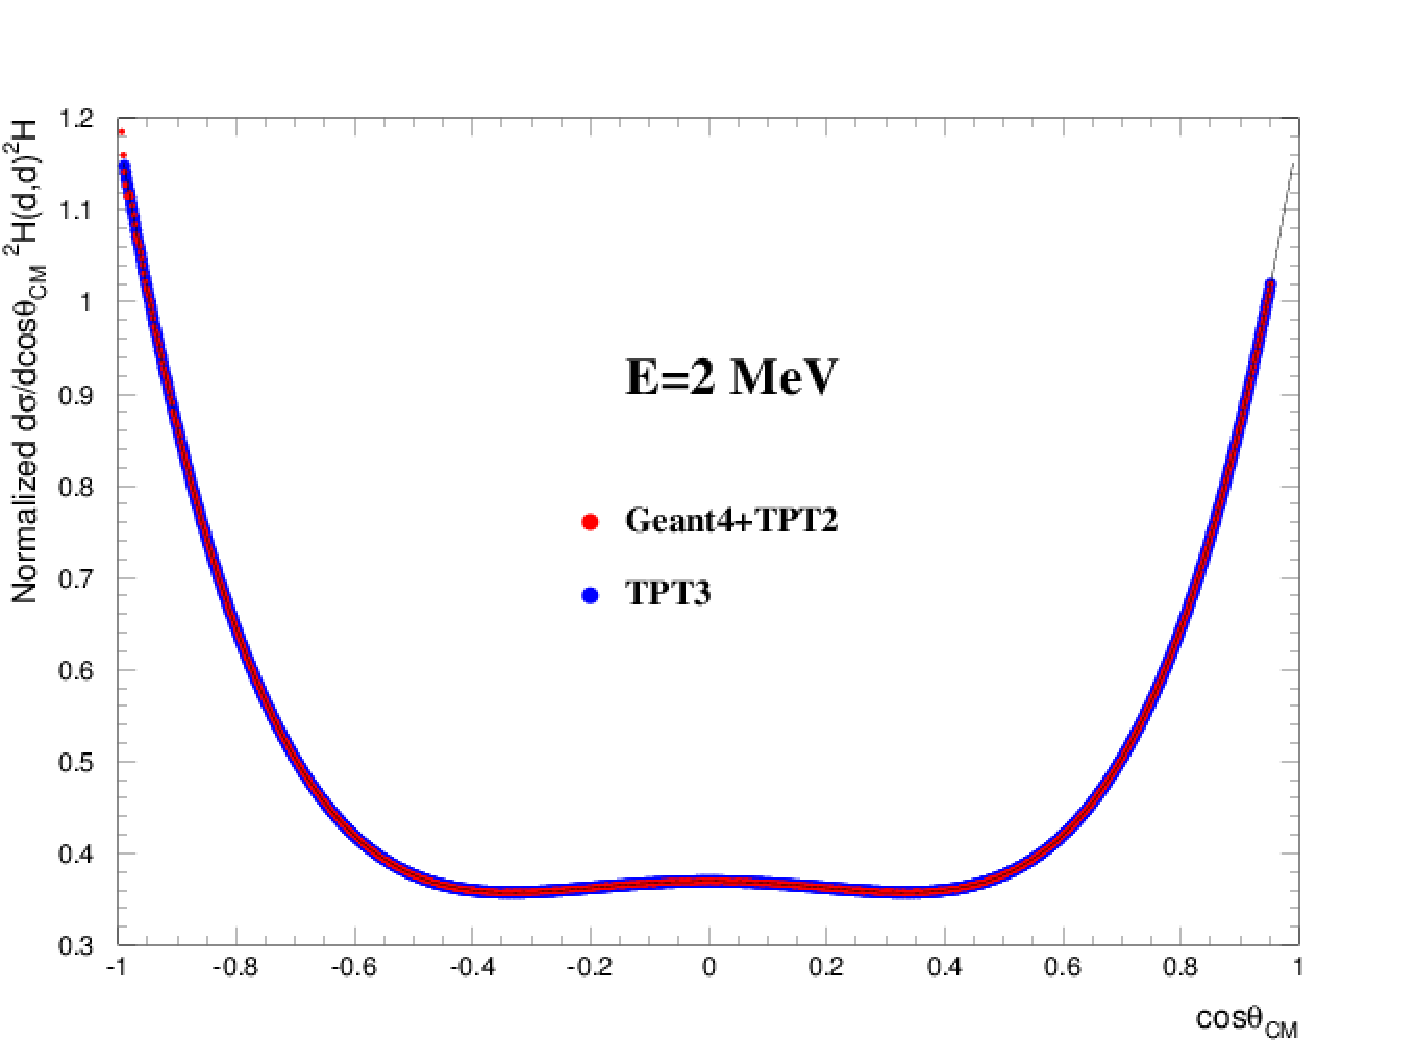
\includegraphics[width=0.99\linewidth]{images/validation_thermonuclear_2mev_2billion.pdf}
  }
  \caption{Сравнение гистограмм нормированного дифференциального сечения, полученных при моделировании неупругой D-D реакции в тонкой мишени дейтерида титана при запуске 2 миллиардов дейтронов с помощью Geant4 и разрабатываемого параллельного программного кода TPT3.}
  \label{fig:ValidationThermonuclear2mev2billionParticles}
\end{figure}	
	
	Некоторое отличие между результатами моделирования наблюдается в области обратного рассеяния около    $\cos{ \left( \theta_{CM} \right) }=-1$.
	Оно показано на Рис. ~\ref{fig:CompareTPT2WithTPT32billionParticles}.
	Как выяснилось, это вызвано тем, что в области $\cos{ \left( \theta_{CM} \right) }=1$ частичные суммы очень мало отличаются от единицы и друг от друга.
	Чтобы увеличить это отличие и для удобства моделирования при в базу данных TPT2 записывались не частичные суммы, а квадратный корень из них.
	Но тогда при розыгрыше $\cos{ \left( \theta_{CM} \right) }$ с помощью случайного числа нужно было брать корень из случайного числа, но в программном комплексе TPT2 бралось случайное число, а не его корень. Это и было причиной ошибки.
	Как видно из Рис. ~\ref{fig:CompareTPT2WithTPT32billionParticles}, этот баг TPT2 исправлен в TPT3. 		И если не рассматривать эту малую область при $\cos{ \left( \theta_{CM} \right) }=-1$, результаты моделирования Geant4 и разрабатываемым параллельным программным комплексом TPT3, везде совпадают с отличной точностью.
	
\begin{figure}[ht]
  {
     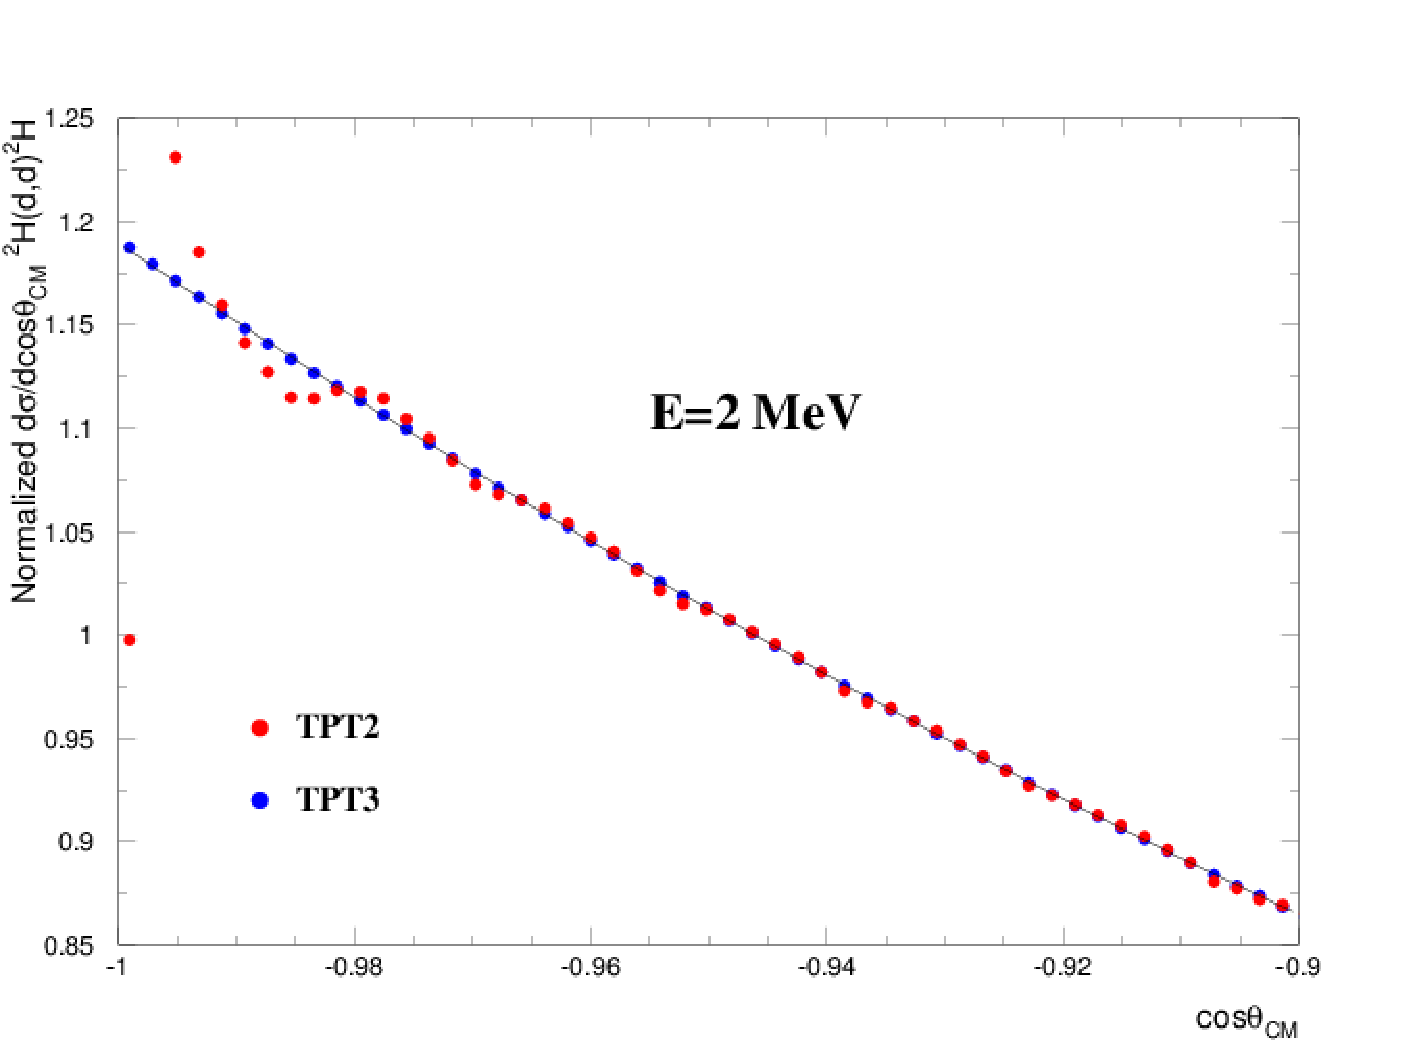
\includegraphics[width=0.99\linewidth]{images/compare_tpt2_with_tpt3_2billion.pdf}
  }
  \caption{Отличие результатов моделирования с помощью Geant4 и с помощью разрабатываемого параллельного программного кода неупругой D-D реакции в тонкой мишени дейтерида титана в районе $\cos{ \left( \theta_{CM} \right) }=-1$ при запуске 2 миллиардов дейтронов.}
  \label{fig:CompareTPT2WithTPT32billionParticles}
\end{figure}	
	

\clearpage{}
\section{Валидация углового распределения упругого D-D рассеяния.}
\label{ValElasticDD}
\
	Для моделирования ионного каскада в мишени из дейтерида титана, вызванного облучением мишени потоком дейтронов, необходимо было также использовать аппроксимацию дифференциального сечения упругого D-D рассеяния, полученную в отчёте [RepIonMat].
	Обычно для моделирования упругого рассения из-за кулоновского барьера и ряда других причин используют просто дифференциальное сечение Резерфордовского рассеяния.
	Особенность данной аппроксимации в том, что она получена для интерференции электромагнитной (Резерфордовское рассеяние) и ядерной (сильное взаимодействие) амплитуд рассеяния.
	Отличие от Резерфордовского дифференциального сечения проявляется в области максимального угла рассеяния $\theta_{CM}=\frac{\pi}{2}$ в системе центра масс (т. к. рассеиваются тождественные частицы, угол рассеяния $\theta_{CM}$ изменяется от 0 до $\frac{\pi}{2}$), что показано на Рис. ~\ref{fig:DifferenceOfElasticDDFromRutherfordDifferentialCrossSection}, где углу рассеяния $\theta_{CM}=\frac{\pi}{2}$ соответствует правая часть оси абсцисс, где $\cos{\theta_{CM}}=0$ и $1-\cos{\theta_{CM}}=1$.
	Т. е. отличие полного дифференциального сечения упругого рассеяния от чисто Резерфордовского наблюдается при рассеянии на большие углы.
	Как видно из Рис. ~\ref{fig:DifferenceOfElasticDDFromRutherfordDifferentialCrossSection}, оно существенно, и его необходимо учитывать при моделировании.
	
\begin{figure}[ht]
  {
     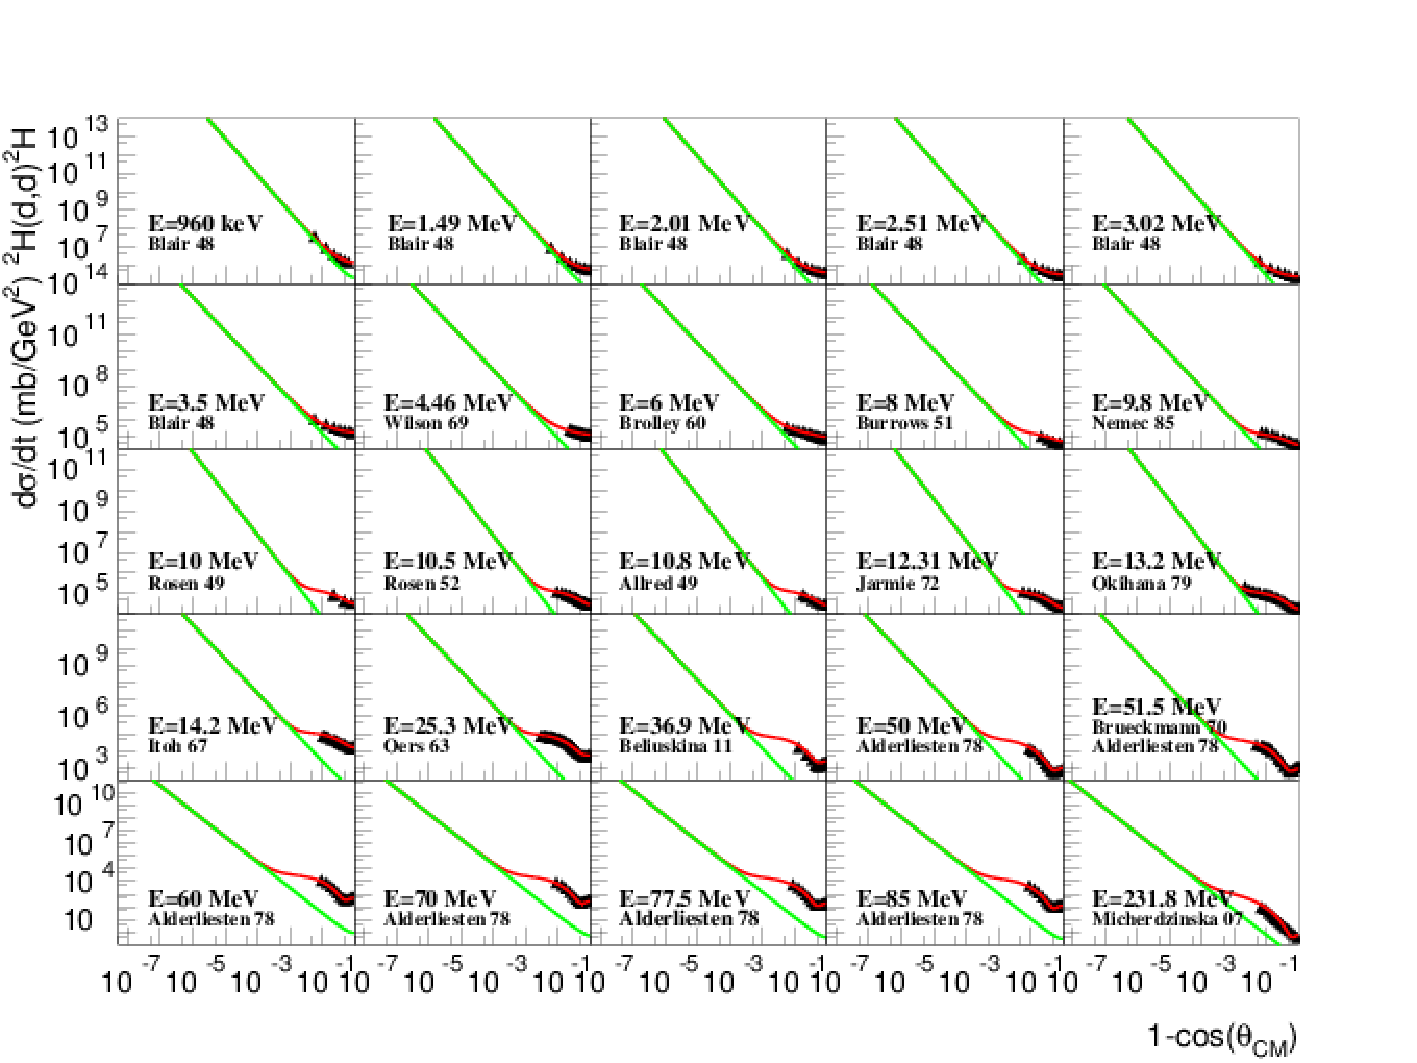
\includegraphics[width=0.99\linewidth]{images/difference_of_elastic_dd_from_rutherford_differential_cross_section.pdf}
  }
  \caption{Отличие дифференциального сечения рассеяния Резерфорда (зелёная кривая) от аппроксимации полного упругого дифференциального сечения рассеяния D-D (красная кривая) при различных кинетических энергиях налетающего дейтрона. Чёрными точками показаны использовавшиеся для аппроксимации экспериментальные данные, бравшиеся из базы ядерных данных EXFOR.}
  \label{fig:DifferenceOfElasticDDFromRutherfordDifferentialCrossSection}
\end{figure}	
	
	В разрабатываемом параллельном программном коде был написан процесс упругого D-D рассеяния, который возвращает сечение и конечное состояние (на вход подаётся налетающий дейтрон, на выходе получается 2 частицы: рассеянный дейтрон и дейтрон отдачи) данной неупругой реакции для налетающего дейтрона.
	Для проверки получающегося в ходе моделирования углового распределения в тонкую мишень дейтерида титана запускались $N_P=100$ миллионов дейтронов с одной из 4 произвольно выбранных кинетических энергий налетающего дейтрона из Рис. ~\ref{fig:DifferenceOfElasticDDFromRutherfordDifferentialCrossSection}: 0.96 МэВ, 10 МэВ, 14.2 МэВ и 231.8 МэВ.
	Сечение неупругой реакции было искусственно поставлено равным максимальному значению переменной типа double языка С++, равному $1.8 \cdot 10^{308}$, так что каждый из запущенных дейтронов участвовал в неупругой реакции в материале мишени, после чего исключался из моделирования, так как было необходимо только собрать гистограмму количества частиц $N_i$, попавших в интервалы лошарифмической шкалы по $1-\cos{\theta_{CM}}$, для того чтобы проверить получающееся на выходе моделирования дифференциальное сечение.
	В качестве оси абсцисс была выбрана величина $1-\cos{\theta_{CM}}$, а не $\cos{\theta_{CM}}$, т. к. выражающая квадрат переданного во взаимодействии переданного импульса мандельстамовская переменная имеет вид $|t|=2\cdot p^2_{CM} \cdot \left( 1- \cos{\theta_{CM}} \right)$, а также потому что $1-\cos{\theta_{CM}}$ изменяется от 0 до 2 и с ней удобнее и нагляднее работать.
	Полученные количества событий в каждом бине $N_i$ делились на полное количество запущенных дейтронов $N_P$ и умножались на полную величину проинтегрированной аппроксимации упругого сечения (получена в отчёте [RepIonMat]) от $10^{-3} \cdot |t|_m$ до $|t|_m$.
	Таким образом, получались величины $\Delta \sigma_i$ в каждом бине.
	За верхний предел интегрирования бралась величина $|t|=2\cdot p^2_{CM}$, а не $|t|_{max}=4\cdot p^2_{CM}$, т. к. рассеивались тождественные частицы и поэтому максимальный угол рассеяния был $\theta_{CM}=\frac{\pi}{2}$.
	Почему за нижний предел интегрирования была выбрана величина $10^{-3} \cdot |t|_m$, будет объяснено ниже в разделе, описывающем реализацию процесса неупругого рассеяния в разрабатываемом программном коде.
	
	Шкала $1-\cos{\theta_{CM}}$ была логарифмической.
	Поэтому, чтобы извлечь величину дифференциального сечения $\frac{d\sigma}{d|t|}$ из полученной гистограммы, нужно было полученные значения $\Delta \sigma_i$ в каждом бине поделить на шаг по $|t|$ в каждом бине $\Delta |t|_i=|t|_{i+1}-|t|_i$, где $i$ изменялось от 0 до $N_{bin}-1$, $N_{bin}$ -- число бинов в гистограмме.
	
	После описанной процедуры моделирования гистограммы отношений величин $\frac{\Delta \sigma_i}{\Delta |t|}$, полученных в ходе моделирования, к точно вычисленным в среднегеометрической середине логарифмического бина по аппроксимации дифференциального сечения упругого D-D рассеяния, полученной в отчёте [RepIonMat], значениям $\frac{d\sigma}{d|t|}$, для кинетических энергий налетающего дейтрона 0.96 МэВ, 10 МэВ, 14.2 МэВ и 231.8 МэВ, показаны на Рис. ~\ref{fig:CheckDDApproximationFillingBinsOfHistogram}.
	Как видно из Рис. ~\ref{fig:CheckDDApproximationFillingBinsOfHistogram}, в пределах погрешности отношение, как и должно быть, равно 1.
	Т. е. угловое распределение упругого D-D рассеяния в разрабатываемом программном коде моделируется должным образом.
	
\begin{figure}[ht]
  {
     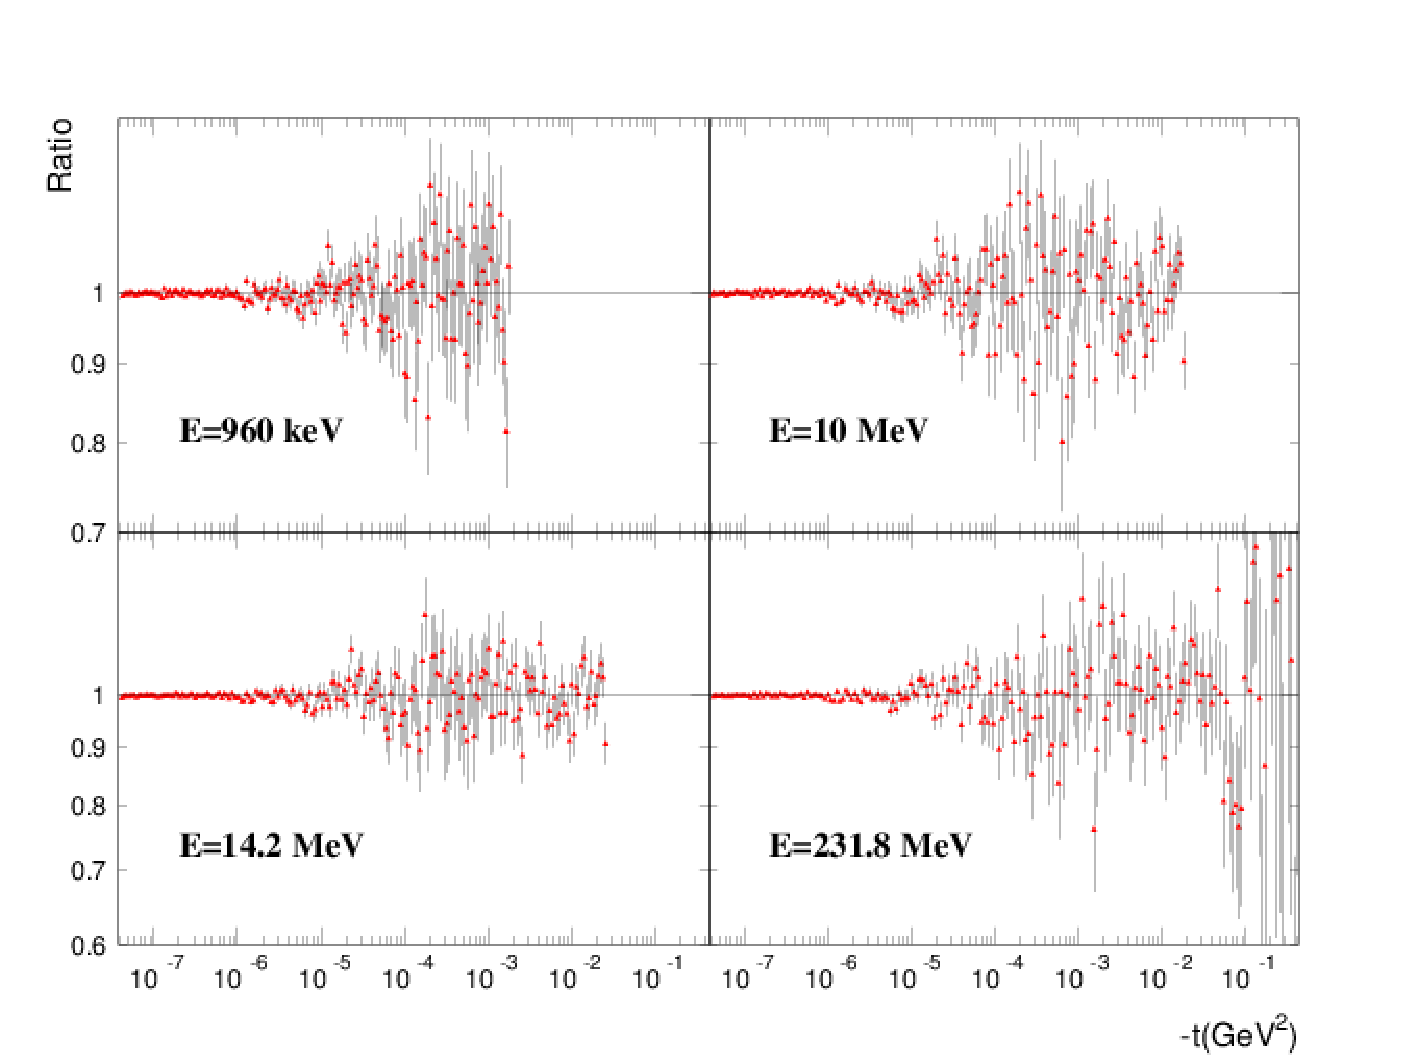
\includegraphics[width=0.99\linewidth]{images/check_dd_approximation_filling_bins_of_histogram.pdf}
  }
  \caption{Отношение дифференциального сечения упругого D-D рассеяния, полученного в ходе моделирования разрабатываемым параллельным программным кодом, к точной величине $\frac{d\sigma}{d|t|}$, вычисленной по аппроксимации дифференциального сечения упругого D-D рассеяния, полученной в отчёте [RepIonMat], в среднегеометрических серединах логарифмических бинов гистограммы. Кинетические энергии налетающих дейтронов: 0.96 МэВ, 10 МэВ, 14.2 МэВ и 231.8 МэВ.}
  \label{fig:CheckDDApproximationFillingBinsOfHistogram}
\end{figure}


\clearpage{}
\section{Валидация энергетической зависимости линейных погонных потерь энергии $\frac{dE}{dx}$ ионов в дейтериде титана.}
\label{ValdEdx}
\subsection{Кривые энергетических потерь $\frac{dE}{dx}$ для ионов дейтерия и титана в дейтериде титана.}
\label{ValdEdx1}

	Средняя мера энергетических потерь заряженных частиц в веществе обозначается величиной $\frac{dE}{dx}$, равной усреднённым энергетическим потерям заряженной частицы с заданной кинетической энергией от всех взаимодействий и физических процессов, в которых она участвует, на единицы дины её пути в веществе.
	Обычно зависимость кривой энергетических потерь заряженных частиц в веществе $\frac{dE}{dx}$ от кинетической энергии налетающей частицы $T_{LS}$ задаётся формулой Бете-Блоха:
	
\begin{equation}
  \label{BetheBloch}
    \frac{dE}{dx}=\frac{Kz^2Z}{A\beta^2}\left[\frac{1}{2}ln\left(\frac{2m_ev^2\gamma^2T_{max}}{I^2}          \right)-\beta^2-\frac{\delta(\beta\gamma)}{2}\right],
\end{equation}
  	где $K=0.307075\frac{MeV\cdot cm^2}{mol}$, $z$ -- заряд налетающего иона, $Z$ -- заряд ядер вещества, $A$ -- атомный вес вещества, $m_e$ -- масса электрона, скорость налетающей частицы $v=c\beta$, величина $T_{max}$ определяет максимальную энергию, которую может передать налетающая частица свободному электрону при столкновении и $I$ -- средний потенциал ионизации, который обычно является подгоночным параметром при аппроксимации экспериментальных данных.
  	Коэффициент $\delta(\beta\gamma)$ отвечает за параметризацию эффекта плотности.
  
  	Как видно из формулы (\ref{BetheBloch}), если рассматриваются кривые $\frac{dE}{dx}$ для разных ионов в одном и том же веществе, то в первом приближении, если не учитывать отличие слагаемых в скобках, можно считать, что коэффициент отличия есть $\frac{z^2}{\beta^2}$.
  	Т. к. $c=1$, то $\beta^2=v^2=\frac{T_{LS}}{m}$, где $m$ -- масса частицы, рассеивающейся в мишени.
  
  	Т. е. если, допустим, известна кривая энергетических потерь $\frac{dE}{dx}$ для ионов дейтерия в дейтериде титана, то по ней можно получить $\frac{dE}{dx}$ для титана в дейтериде титана используя скейлинговый коэффициент $\frac{z^2}{\beta^2}$.
 	В процессе моделирования ионного каскада  в мишени из дейтерида титана, инициированного облучением мишени потоком дейтронов с кинетической энергией $T_{LS}=100$ кэВ, присутствуют 2 процесса, приводящие к появлению отличных от дейтронов частиц.
 	Это реакция неупругого рассеяния, имеющая 2 выходных канала: n + $^3_2He$ и p + t, и упругое ион-ионное рассеяние, в результате которого могут появиться либо дейтрон, либо ион титана.
 	Т. к. вероятность непругой реакции по отношению к упругому ион-ионному рассеянию при $T_{LS}=100$ кэВ, равняется $10^{-5}$, то в первую очередь, конечно, нужно знать кривые энергетических потерь $\frac{dE}{dx}$ для ионов дейтерия и титана в дейтериде титана.
  
 	В базе данных для протонов PSTAR даны аппроксимации электронных потерь $\frac{dE}{dx}$ для протонов в дейтериде титана.
 	Из-за крайне малого времени релаксации не представляется возможным измерить зависимость $\frac{dE}{dx}$ для изотопов водорода в дейтериде титана.
 	Таких экспериментальных данных просто нет.
 	Также не удалось найти и данных по $\frac{dE}{dx}$ для ионов титана в дейтериде титана, их тоже не представляется возможным экспериментально измерить из-за тождественности налетающих частиц и частиц материала мишени.
  
 	Поэтому была взята аппроксимация $\frac{dE}{dx}$ для протонов в титане, показанная на Рис. ~\ref{fig:DeDxInTiD2Plot}.
 	Эти точки аппроксимации из базы данных PSTAR в свою очередь были проаппроксимированы нами в виде непрерывной функции:
  
\begin{equation}
  \label{dEdxHInTiD2Approximation}    
	  \frac{1}{z^2} \cdot \frac{dE}{dx}=\frac{1.007}{ \left( \frac{T_{LS}}{m} \right)^{0.74}+1.29 \cdot 10^{-5} \cdot \left( \frac{T_{LS}}{m} \right)^{-0.52} } + 6.74 \cdot \left[ F_4 \left( \frac{T_{LS}}{m} \right) \right]^{2.02},
\end{equation}

	где $F_n$ рекурсивно определяется следующим образом: $F_0=\ln{\left( 1+\frac{T_{LS}}{m} \right)}$, $F_1=\ln{\left( 1+F_0 \right)}$, $F_2=\ln{\left( 1+F_1 \right)}$ и т. д.
	Аппроксимирующая функция (\ref{dEdxHInTiD2Approximation}) изображена на Рис. ~\ref{fig:DeDxInTiD2Plot} розовой кривой. Аппроксимирующие $\frac{dE}{dx}$ кривые для дейтронов и ионов титана изображены на Рис. ~\ref{fig:DeDxInTiD2Plot} синим и красным цветом.
	Они были получены в результате скейлинга функции (\ref{dEdxHInTiD2Approximation}) по оси ординат на коэффициент $z^2$ квадрата заряда иона, для которого $\frac{dE}{dx}$ необходимо вычислить, и по оси абсцисс на коэффициент $\frac{m}{m_D}$, где $m_D$ -- масса дейтрона, равная 1875.6 МэВ, а $m$ -- масса иона, для которого необходимо рассчитать $\frac{dE}{dx}$. 
  
\begin{figure}[ht]
  {
     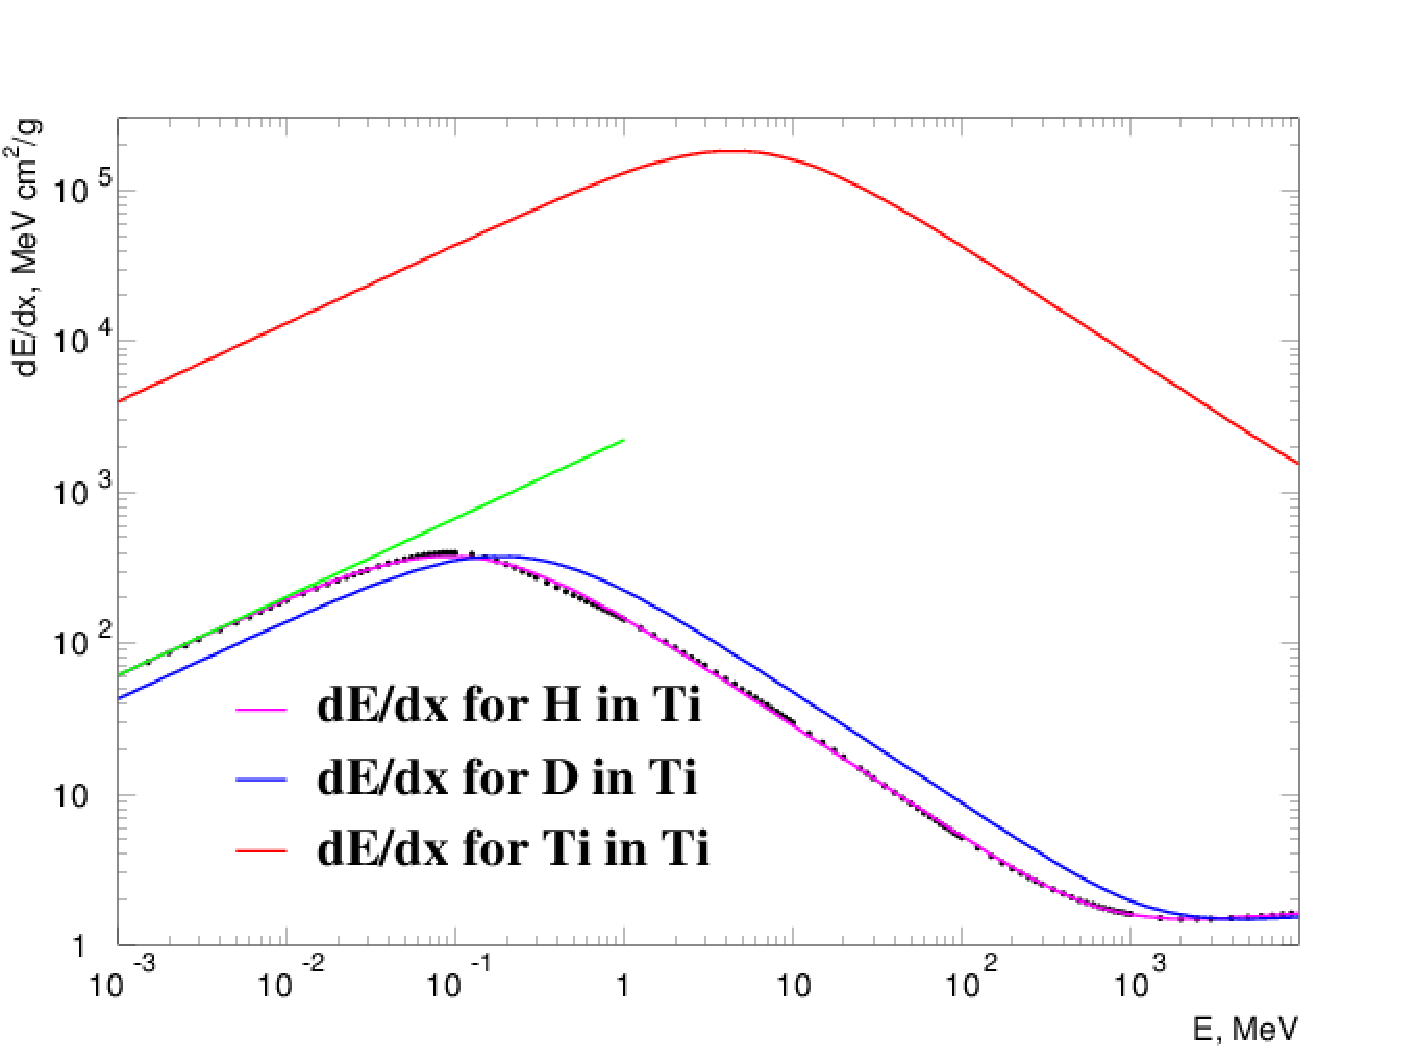
\includegraphics[width=0.99\linewidth]{images/dedx.pdf}
  }
  \caption{Кривые энергетических потерь $\frac{dE}{dx}$ для протонов, дейтронов и ионов титана в дейтериде титана. Чёрные точки -- аппроксимация $\frac{dE}{dx}$ для протонов в дейтериде титана, взятая из базы данных PSTAR для протонов. Розовая кривая $\frac{dE}{dx}$ для протонов -- аппроксимация этих данных.Остальные -- синяя для дейтронов и красная для протонов -- кривые $\frac{dE}{dx}$ получены умножением розовой аппроксимационной кривой на скейлинговый фактор $\frac{z^2 \cdot m}{T_{LS}}$. Зелёная кривая показывает как $\frac{dE}{dx}$ экстраполируется к $T_{LS}=0$ МэВ, т. к. экспериментальной аппроксимации энергетических потерь в области малых энергий нет.}
  \label{fig:DeDxInTiD2Plot}
\end{figure}

	Зелёной кривой показана экстраполяция $\frac{dE}{dx}$ для протонов в дейтериде титана в область малых энергий.
	Известно, что по Линхарду эта экстраполяция должна быть $\sim \sqrt{v}$.
	Если в (\ref{dEdxHInTiD2Approximation}) сделать предельный переход $T_{LS} \to 0$, получается следующая функция экстраполяции $\frac{dE}{dx}$ в область малых $T_{LS}$:

\begin{equation}
  \label{dEdxLinhardExtrapolationInSmallTls}	
  \frac{dE}{dx}^{extra}=7.79 \cdot 10^4  \cdot z^2 \left( \frac{T_{LS}}{m} \right)^{0.52}.
\end{equation}

\subsection{Сравнение быстродействия вычисления $\frac{dE}{dx}$ по таблице и по функции.}
\label{ValdEdx2}	

	При моделировании в разрабатываемом параллельном программном коде линейных потерь энергии частиц в материле мишени есть 2 возможности: вычислять значение $\frac{dE}{dx}$ по таблице и по аппроксимирующей $\frac{dE}{dx}$ функции.
	
	Как видно из Рис. ~\ref{fig:DeDxInTiD2Plot}, у нас в распоряжении имеются чёрные точки аппроксимации электронной $\frac{dE}{dx}$ протонов в дейтериде титана, взятые из базы данных PSTAR.
	Они соответствуют таблице ($T_{LSi}$, $\frac{dE}{dx}_i$), где номер бина $i$ изменяется от 0 до 131, т. е. всего 132 пары величин ($T_{LS}$, $\frac{dE}{dx}$).
	При помощи описанного скейлинга из точек для протонов можно получить точки аппроксимации для дейтронов и ионов титана.
	Тогда по ним можно будет находить значение $\frac{dE}{dx}$ при заданной кинетической энергии $T_{LS}$ налетающей частицы следующим образом: сначала с помощью бинарного поиска находится бин $i$, куда частица попала по кинетической энергии $T_{LS}$.
	Далее, при помощи линейной интерполяции можно найти значение $\frac{dE}{dx}=\frac{dE}{dx}_i+\frac{ T_{LS}-T_{LSi} }{ T_{LSi+1}-T_{LSi} } \cdot \left( \frac{dE}{dx}_{i+1}-\frac{dE}{dx}_{i} \right)$.
	Если $T_{LS}$ было больше верхней границы $T_{LSi}$, т. к. данных аппроксимации нет, возвращался 0, если $T_{LS}$ был ниже нижней границы $T_{LSi}$, возвращалось значение $\frac{dE}{dx}$, вычисленное по функции (\ref{dEdxLinhardExtrapolationInSmallTls}) экстраполяции $\frac{dE}{dx}$ к нулю по $T_{LS}$.
	
	 Или же можно было использовать полученную функцию (\ref{dEdxHInTiD2Approximation}) аппроксимации $\frac{dE}{dx}$ ионов в дейтериде титана и точно по ней вычислять значение средних потерь энергии.
	 
	 Задача была проверить, какой из этих 2 способов вычисления $\frac{dE}{dx}$ работает быстрее при параллельном моделировании большого количества частиц.
	 Проверка проводилась для $\frac{dE}{dx}$ дейтронов в дейтериде титана, но очевидно, что точно такой же результат будет и для протонов, и для ионов титана в дейтериде титана.
	 В диапазоне $T_{LS}$ от $T^{min}_{LS}=200$ эВ до $T^{max}_{LS}=20$ МэВ с линейным шагом $\Delta T_{LS}=\frac{T^{max}_{LS}-T^{min}_{LS}}{N_P}$, где $N$ -- число вызовов функции, вычисляющей $\frac{dE}{dx}$, и при каждом вызове для очередного значение кинетической энергии вычислялось значение $\frac{dE}{dx}$.
	 Вычисления проводились параллельно и с использованием векторизации. Сначала запускалась функция, вычислявшая $\frac{dE}{dx}$ по таблице, затем - по функции (\ref{dEdxHInTiD2Approximation}).
	 Замерялось время работы программы и делилось на число вызовов. Таким образом, получалось время 1 вызова функции, вычисляющей $\frac{dE}{dx}$, в зависимости от суммарного числа вызовов $N$.
	 И такие измерения были проведены в широком диапазоне по $N$ на различных вычилительных платформах, имеющихся во ВНИИА.
	 
	 Результат представлен на Рис. ~\ref{fig:CompareParallellydEdx}.
	 Как из него видно, самой производительной оказалась видеокарта Nvidia Titan V.
	 На ней при суммарных $10^{11}$ вызовах функции вычисления $\frac{dE}{dx}$ отношение времени вычисления $\frac{dE}{dx}$ по таблице и по функции выходит на константу, равную 10.
	 Процессор ПК Intel Core i7-3770 почти в 3.7 раз более производителен при вычислении $\frac{dE}{dx}$ по таблице, чем по функции при $N \geq 10^8$.
	 64-ядерный процессор Intel Xeon Phi KNL при $N \geq 2\cdot 10^9$ в 3.1 раз быстрее работает при вычислении $\frac{dE}{dx}$ по таблице, чем по функции.
	 Самый быстрый 36-ядерный (2 процессора по 18 ядер, соединённые вместе) узел кластера VKPP достигает отличия в производительности при вычислении по таблице и по функции в 4.4 раза при $N$ порядка $10^{10}$.
	 Оказалось, что старая довольно слабая видеокарта Nvidia GTX GeForce 650 Ti, установленная в корпусе ПК с CPU Intel Core i7, на данной задаче показывает более высокую производительность (примерно в 1.2 раза быстрее), чем центральный процессор.
	 Окончательное сравнение быстродействия различных вычислительных платформ при параллельном счёте, использующем векторизацию, представлено в таблице ниже.
	 Т. к. наименьшей производительность в данном тесте, как видно из Рис. ~\ref{fig:CompareParallellydEdx}, обладает CPU Intel Core i7, в данной таблице представлены отношения времени выполнения функции, возвращающей $\frac{dE}{dx}$, на CPU Core i7 к временам её выполнения на интересующих вычислительных платформах при заданных $N$.
	 
	 \begin{tabular}{|c|c|c|}
	 \hline 
	 CPU/GPU & Таблица & Функция \\ 
	 \hline 
	 Geforce 650 Ti & 1.2 & 0.7 \\ 
	 \hline 
	 KNL & 5 & 6.1 \\ 
	 \hline 
	 36-ядерный узел VKPP & 7.4 & 6.3 \\ 
	 \hline 
	 Titan V & 180 & 68 \\ 
	 \hline 
	 \end{tabular} 
	 
	При уменьшении числа вызовов на всех вычислительных платформах за исключением KNL и 36-ядерного узла VKPP вычиcление $\frac{dE}{dx}$ по функции оказывается немного быстрее вычисления по таблице.
	Для KNL при уменьшении N они совпадают, а для 36-ядерного узла VKPP почему-то оказывается значительно быстрее вычисление по таблице.
	Вероятно, это связано в процессорной архитектурой, ведь на 36-ядерном узле VKPP 2 18-ядерных процессора соединены вместе.
	Также влияние может оказывать размер кэшей, вероятно, из-за большого количества ядер они там урезанные.
	
	То, что GPU Titan V позже всех вычислительных платформ выходит на константу времени вызова функции говорит о том, что она обладает самым большим из всех представленных вычислительных платформ потенциалом для высоконагруженных параллельных вычислений и оказывается полностью загруженной лишь при числе вызовов, большем $2 \cdot 10^{11}$. 
	 
	Как видно из Рис. ~\ref{fig:CompareParallellydEdx}, при параллельном счёте и использовании векторизации однозначно быстрее оказывается вычислять $\frac{dE}{dx}$ по таблице используя бинарный поиск и линейную интерполяцию, чем точно считать значение по аппроксимирующей функции.
	 

\begin{figure}[ht]
  {
     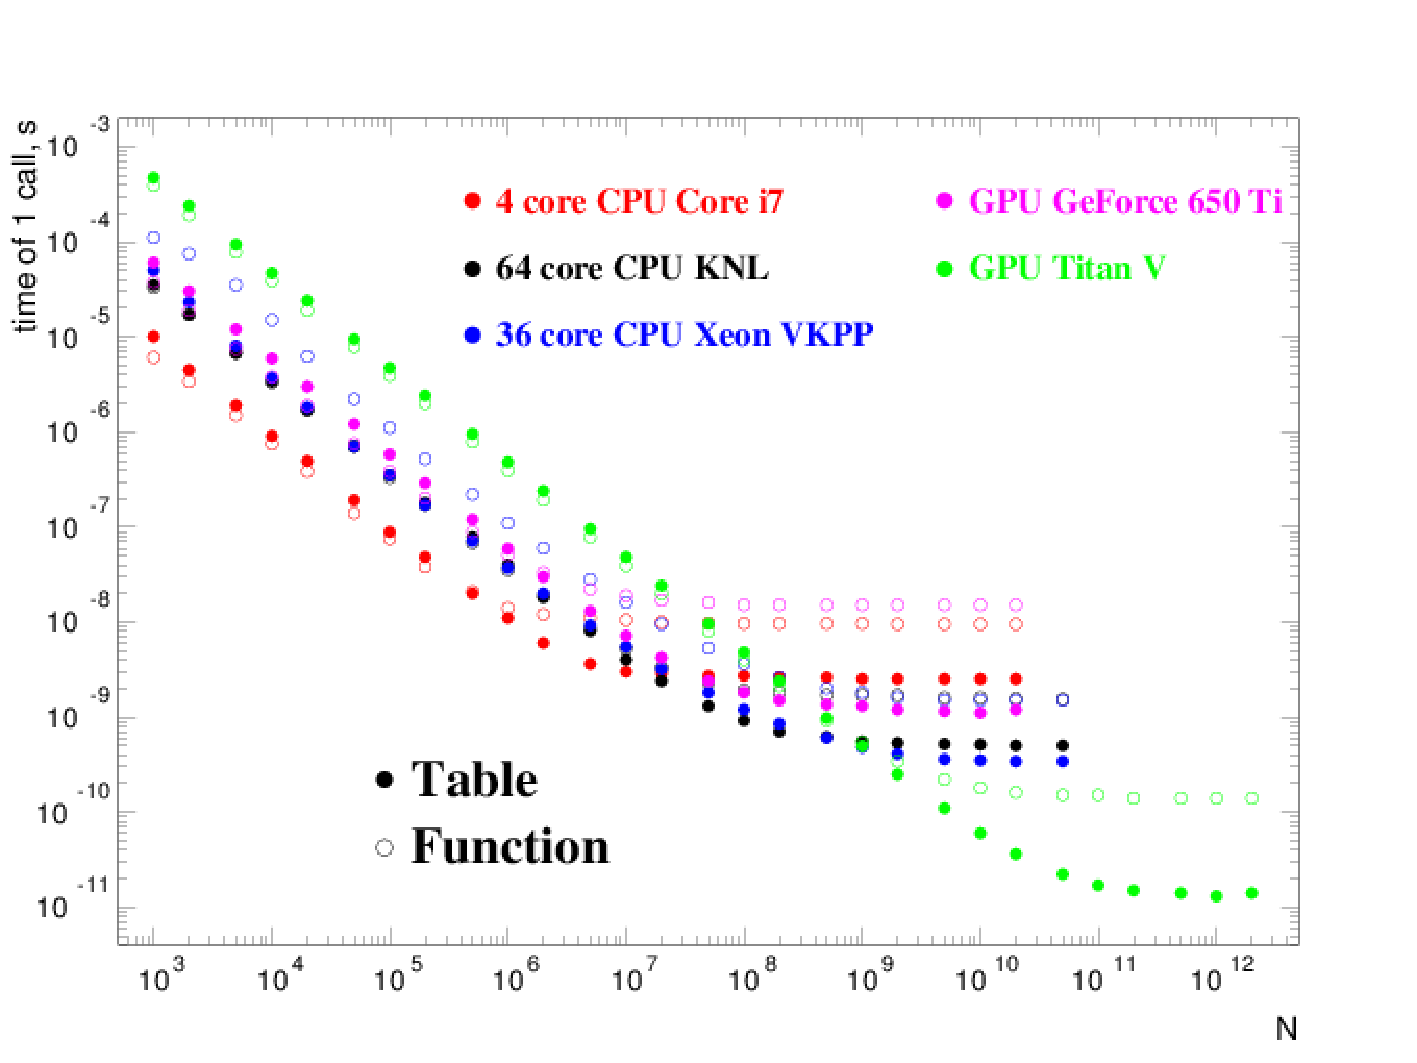
\includegraphics[width=0.99\linewidth]{images/compare_parallelly_dEdx.pdf}
  }
  \caption{Быстродействие программной функции вычисления $\frac{dE}{dx}$ по таблице (чёрные круги) и по аппроксимационной функции (\ref{dEdxHInTiD2Approximation}) (чёрные окружности) на различных вычислительных платформах, имеющихся во ВНИИА, в зависимости от числа вызовов программной функции в параллельном расчёте. Данный параллельный расчёт использует максимально возможное распараллеливание по потокам и векторизацию.}
  \label{fig:CompareParallellydEdx}
\end{figure}

	Также было интересно посмотреть как изменится быстродействие и соотношение производительностей при однопоточном расчёте без использования векторизации.
	Данные измерения были произведены, и их результат представлен на Рис. ~\ref{fig:CompareSequentiallydEdx}.
	
\begin{figure}[ht]
  {
     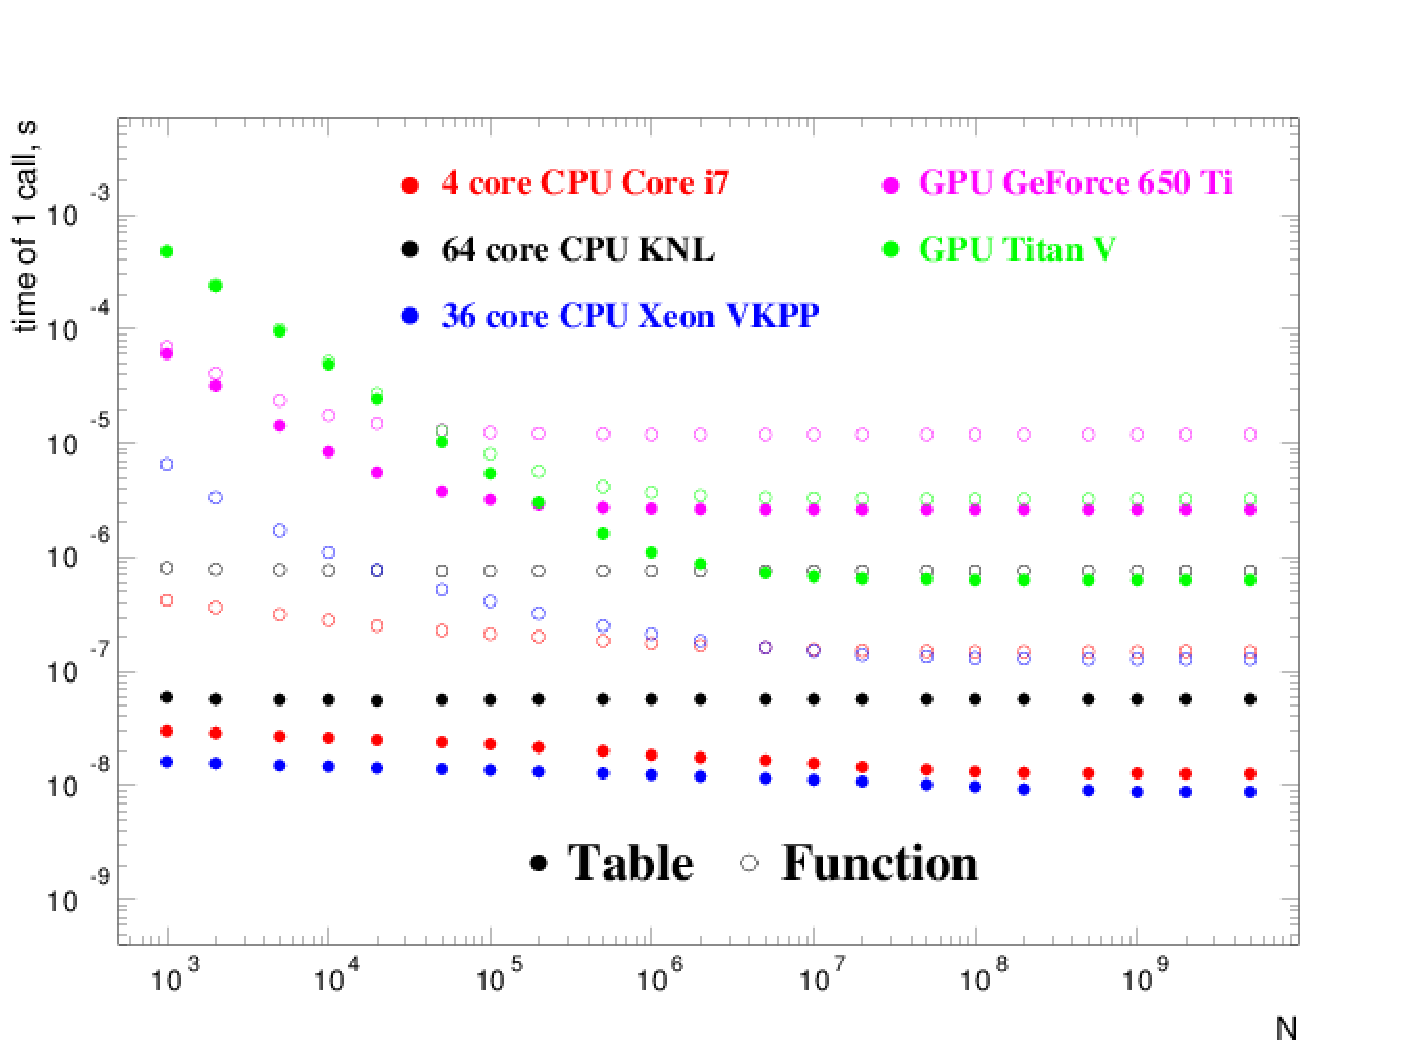
\includegraphics[width=0.99\linewidth]{images/compare_sequentially_dEdx.pdf}
  }
  \caption{Быстродействие программной функции вычисления $\frac{dE}{dx}$ по таблице (чёрные круги) и по аппроксимационной функции (\ref{dEdxHInTiD2Approximation}) (чёрные окружности) на различных вычислительных платформах, имеющихся во ВНИИА, в зависимости от чила вызовов программной функции в однопоточном расчёте без использования векторизации.}
  \label{fig:CompareSequentiallydEdx}
\end{figure}

	За исключением GPU, 36-ядерного узла кластера VKPP и процессора Intel Core i7, все остальные платформы показывают почти константное время счёта при любом $N$.
	На GPU при уменьшении $N$ наблюдается увеличение времени вызова при вычислении $\frac{dE}{dx}$ и по таблице, и по функции.
	Вероятно, этот эффект связан с особенностями архитектуры GPU. Почему-то он наблюдается и при вычислении $\frac{dE}{dx}$ по аппроксимирующей функции на 36-ядерном узле кластера VKPP. 
	
	При запуске последовательного и невекторизованного кода самую слабую производительность показала GPU GeForce 650 Ti.
	Поэтому ниже приведена таблица, в которой представлены отношения времени вызова функции, вычисляющей $\frac{dE}{dx}$, на GPU GeForce 650 Ti, к времени её вызова на интересующей вычислительной платформе при заданном $N$.

	 \begin{tabular}{|c|c|c|}
	 \hline 
	 CPU/GPU & Таблица & Функция \\ 
	 \hline 
	 Titan V & 4.1 & 3.7 \\ 
	 \hline 
	 KNL & 45 & 16 \\ 
	 \hline 
	 Core i7 & 206 & 80.1 \\ 
	 \hline 
	 36-ядерный узел VKPP & 298 & 93 \\ 
	 \hline 
	 \end{tabular} 

	Т. е. при запуске последовательного кода без векторизации самыми быстрыми оказались центральные процессоры ПК Intel Core i7-3770 и 36-ядерного процессора Intel Xeon E5-2697 узла кластера VKPP и самыми медленными видеокарты.
	Это понятно: у этих CPU самые большие тактовые частоты (базовые частоты у E5 – 2.3 ГГц, у Core i7 – 3.4 ), а у GPU самые медленные (у GPU GeForce 650 Ti -- 1.1ГГц, у Titan V -- 1.5 ГГц).
	Т. к. код исполняется последовательно, то фактически его быстродействие определяется тактовой частотой процессора, на котором он исполняется.
	
	Из только что проведённого исследования производительности вычисления значения $
\frac{dE}{dx}$ по таблице при помощи бинарного поиска и линейной интерполяции и по аппроксимирующей функции однозначно следует, что при высоконагруженных параллельных расчётах значительно быстрее работает вычисление $\frac{dE}{dx}$ по таблице, чем по функции.
	Поэтому в разрабатываемом разрабатываемом параллельном программном коде все операции вычисления $\frac{dE}{dx}$ выполнялись с помощью бинарного поиска и линейной интерполяции по таблице аппроксимации линейных электронных потерь энергии, взятой из базы данных PSTAR и преобразованной с помощью описанного скейлинга.
	Если же величина кинетической энергии дейтрона была меньше минимального значения $T_{LS}$ в полученной с помощью скейлинга базе данных, то значение $\frac{dE}{dx}$ вычислялось при помощи эктраполяции (\ref{dEdxLinhardExtrapolationInSmallTls}) в область малых $T_{LS}$.

  
  

\clearpage{}
\section{Программная реализация процессов физических взаимодействий.}
\subsection{Описание типового дискретного процесса рассеяния частицы в среде.}
\label{TypicalPhysicalProcessDescription}

	Реализация всех процессов упругого ион-ионного и D-D рассеяния, неупругой D-D реакции, а в будущем и других физических процессов, делалась единообразным образом.
	
	На вход программе подавался вектор 4-импульса $\vec{p}\,^{inc}_{LS}$=($p_x$, $p_y$, $p_z$, $E^{inc}_{LS}$) рассеивающейся или участвующей в реакции частицы и её PDG-код, определяющий вид частицы.
	Импульс налетающей частицы $\vec{p}\,_{LS}^{inc}$ =($p_x$,$p_y$,$p_z$,$E^{inc}_{LS}$) переводился из лабораторной системы в систему центра масс следующим образом.
	Т. к. в лабораторной системе ядро мишени -- при моделировании ионного каскада в мишени из дейтерида титана это расположенное в узле кристаллической решётки ядро дейтерия либо титана -- покоилось, то из соотношений Лоренца следовало, что
\begin{equation}
\label{PLStoCM}
\begin{aligned} 
  \vec{p}_{CM} = \gamma \left( \vec{p}\,_{LS}^{inc} - \vec{V}_{CM} \cdot E_{LS}^{inc} \right) = \vec{p}\,_{LS}^{inc} \cdot \frac{M}{\sqrt{s}},
\end{aligned}
\end{equation}
где гамма-фактор равен $\gamma=\frac{E_{LS}^{inc}+M}{\sqrt{s}}$, $\vec{V}_{CM} = \frac{\vec{p}\,_{LS}^{inc}}{E_{LS}^{inc}+M}$ -- скорость системы центра масс, мандельстамовская переменная $s$ определяется выражением

\begin{equation}
  \label{MandelStahmSVariableDefinition}    
  s=m^2+2 \cdot E^{inc}_{LS} \cdot M + M^2,
\end{equation}
	а $m$ и $M$ -- массы налетающей частицы и ядра отдачи соответственно, вычисляемые по их PDG-коду. 

	Таким образом, по импульсу $\vec{p}\,_{LS}^{inc}$ и энергии $E_{LS}^{inc}$ налетающей частицы в лабораторной системе получались импульс в системе центра масс $\vec{p}_{CM}$ и энергия налетающей частицы в системе центра масс $E^{inc}_{CM}=\sqrt{m^2+p_{CM}^2}$.
	
	Далее, необходимо было разыграть с помощью случайного числа и извлечь из соответствующей типу взаимодействия специально подготовленной базы данных значение косинуса угла рассеяния в системе центра масс $\cos{\theta_{CM}}$.
	
	После того как угол рассеяния в системе центра масс $\theta_{CM}$ был посчитан, импульс в системе центра масс после рассеяния определялся как
\begin{equation}
\label{CMMomentumFin}
\begin{aligned} 
  {\vec{p}_{CM}}^{fin} = p_{CM}\cdot\left(\cos{\theta_{CM}} \cdot \vec{e}_1 + \sin{\phi} \cdot   \sin{\theta_{CM}} \cdot \vec{e}_2 +  \cos{\phi} \cdot \sin{\theta_{CM}} \cdot \vec{e}_3\right),
\end{aligned}
\end{equation}
где $\vec{e}_1$ -- единичный вектор в направлении $\vec{p}_{CM}$, $\vec{e}_2$ и $\vec{e}_3$ -- произвольные взаимно перпендикулярные единичные вектора, перпендикулярные $\vec{e}_1$, а $\phi$ -- случайный угол от $0$ до $2\pi$.
	
	В случае упругого рассеяния $\vec{p}_{CM}$ в результате взаимодействия не меняется по модулю, лишь по направлению.
	Но при реакции неупругого D-D рассеяния, т. к. взаимодействие неупругое, $p_{CM}$ уменьшается.
	И это также необходимо учитывать. 
	
	После осуществления взаимодействия в системе центра масс необходимо было перевести $\vec{p}\,^{fin}_{CM}$ обратно в лабораторную систему координат.
	Т. к. при преобразовании Лоренца изменяется только продольная (имеющая направление вдоль $\vec{V}_{CM}$) компонента вектора импульса, поперечная же остаётся неизменной, то необходимо было найти компоненту конечного вектора импульса в системе центра масс $\vec{p}\,^{fin}_{CM}$ вдоль $\vec{V}_{CM}$, а значит, вдоль $\vec{p}_{CM}$, т. к. ядро мишени покоится.
	Эта компонента, очевидно, равна $\vec{p}\,^{fin \parallel \vec{V}_{CM}}_{CM}=\vec{p}\,^{fin}_{CM} \cdot \frac{\vec{p}_{CM}}{p_{CM}}$.
	Компонента, перпендикулярная $\vec{p}_{CM}$, есть $\vec{p}\,^{fin \bot \vec{V}_{CM}}_{CM}=\vec{p}\,^{fin}_{CM}-\vec{p}\,^{fin \parallel \vec{V}_{CM}}_{CM}$.
	Для перевода $\vec{p}\,^{fin \parallel \vec{V}_{CM}}_{CM}$ из системы центра масс обратно в лабораторную систему использовалось преобразование Лоренца:
	
\begin{equation}
\label{MSlsincMomentumAfter}
\begin{aligned} 
  \vec{p}\,_{LS}^{fin \parallel \vec{V}_{CM}} = \gamma \left( \vec{p}\,^{fin}_{CM} + \vec{V}_{CM} \cdot E^{fin}_{CM} \right),
\end{aligned}
\end{equation}
	где энергия рассеиваемой частицы в системе центра масс после рассеяния есть $E^{fin}_{CM}=\sqrt{m^2+\left( p^{fin}_{CM} \right)^2}$.
	
	Конечный импульс налетающей частицы находился исходя из того, что $\vec{p}\,^{fin \bot \vec{V}_{CM}}_{CM}$ не менялся при переходе между системами координат, и был равен:
	
\begin{equation}
\label{LSincMomentumAfter}
\begin{aligned} 
  \vec{p}\,_{LS}^{fin} = \vec{p}\,_{LS}^{fin \parallel \vec{V}_{CM}} + \vec{p}\,^{fin \bot \vec{V}_{CM}}_{CM}.
\end{aligned}
\end{equation}	
	
	Конечный импульс ядра мишени в лабораторной системе находился из закона сохранения импульса:
\begin{equation}
\label{LStargetMomentumAfter}
\begin{aligned} 
  \vec{p}\,_{LS}^{fin\,target} = \vec{p}\,_{LS}^{inc} - \vec{p}\,_{LS}^{fin}.
\end{aligned}
\end{equation}
	Полные энергии частиц изменялись как $E_{LS}^{fin}=\sqrt{m^2+\left( p_{LS}^{fin} \right)^2 }$ и $E_{LS}^{fin\,target}=\sqrt{M^2+\left( p_{LS}^{fin\,target} \right)^2 }$.
  
	Таков схематически единообразный алгоритм написания физических процессов упругой и неупругой ядерной реакции.
	По большому счёту, единственным отличием являются различные угловые распределения дифференциальных сечений физических процессов и изменение $p_{CM}$ в ходе неупругих взаимодействий.
	
\subsection{Реализация дискретного процесса неупругой D-D реакции.}
\label{InelasticDDReactionRealization}

	Интегральные сечения неупругой D-D реакции определяется выражениями (\ref{InelasticDDNHe3ChannelIntegralCrossSection}) и (\ref{InelasticDDPTChannelIntegralCrossSection}), дающими значение интегрального сечения одного из 2 каналов неупругой D-D реакции в барнах при данной кинетической энергии налетающего дейтрона в системе центра масс $T_{LS}$ в лабораторной системе координат.
	
	Полное сечение реакции неупругого рассеяния определяется как сумма интегральных сечений обоих каналов неупругой D-D реакции при данной кинетической энергии налетающего дейтрона $T_{LS}$, умноженная на коэффициент $\frac{2}{3}$, равный количественной доле атомов дейтерия в молекуле $TiD_2$.
	
	При розыгрыше 4-импульсов налетающей частицы и ядра мишени при неупругой D-D реакции угловые зависимости дифференциального сечения неупругой D-D реакции определяются с помощью базы данных TPT, куда в свою очередь они были записаны в виде нормированных частичных сумм интегралов от полиномов Лежандра, коэффициенты которых приведены в базе данных ENDF-6.
	Например, при $T_{LS}=2$ МэВ нормированное дифференциальное выглядит как показано на Рис. ~\ref{fig:ValidationThermonuclear2mev2billionParticles}.
	
	Т. к. реакция неупругая, импульс в системе центра масс $p_{CM}$ после взаимодействия изменяется как [формула (38.16) стр. 321 боьшая книга PDG]
	
\begin{equation}
\label{PCMInelasticDDAfterNHe3}
\begin{aligned} 
  p\,_{CM}^{fin} = \frac{ \sqrt{ \left( s-\left( m_n + m_{^3_2He}\right)^2 \right) \cdot \left( s-\left( m_n - m_{^3_2He} \right)^2 \right) } }{2\cdot \sqrt{s}}
\end{aligned}
\end{equation}

	для выходного канала n+$^3_2$He неупругой реакции D-D и как

\begin{equation}
\label{PCMInelasticDDAfterPT}
\begin{aligned} 
  p\,_{CM}^{fin} = \frac{ \sqrt{ \left( s-\left( m_p + m_t\right)^2 \right) \cdot \left( s-\left( m_p - m_t \right)^2 \right) } }{2\cdot \sqrt{s}}
\end{aligned}
\end{equation}

	для её выходного канала p+t.
	Здесь мандельстамовская переменная $s$ определяется выражением (\ref{MandelStahmSVariableDefinition}), а $m_n$, $m_p$, $m_t$ и $m_{^3_2He}$ -- массы нейтрона, протона, тритона и ядра $^3_2He$ соответственно.
	
	Соответственно, если на входе данному процессу должен подаваться налетающий дейтрон, то на выходе будут 2 частицы: либо n+$^3_2He$, либо p+t.
	
	Значение косинуса угла рассеяния в системе центра масс $\cos{\theta_{CM}}$ получалось с помощью равномерно распределённого случайного числа $R$ от 0 до 1, бинарного поиска соответствующего $R$ значения $\cos{\theta_{CM}}$ в базе данных нормированных частичных сумм, соответствующих различным значениям $\cos{\theta_{CM}}$ от -1 до 1, и квадратичной интерполяции значения $\cos{\theta_{CM}}$. 
	

\subsection{Реализация дискретного процесса упругого ион-ионного рассеяния.}
\label{ElasticIonIonScatteringRealization}

	
	В кристаллической решётке дейтерида титана энергия, необходимая для выбивания ионов титана и дейтерия из их равновесного положения в узлах решётки (так называемая ``displacement energy'') $E_{de}$, равняется примерно 25 эВ для титана и примерно 10 эВ для дейтерия.
  	Эти значения используются, например, в программе SRIM \cite{SRIM}, применяющейся для моделирования ионного транспорта, и программах молекулярной динамики.
  	Так как при кинетической энергии налетающей частицы, меньшей указанных значений, не происходит выбивания иона дейтерия либо титана из их равновесного положения в узле кристаллической решётки в результате Резерфордовского рассеяния, можно в качестве дифференциального сечения $\frac{d\sigma_{ms}}{d|t|}$ многократного рассеяния рассматривать дифференциальное сечение Резерфордовского рассеяния при $|t|$ от 0 до
\begin{equation}
\begin{aligned} 
 \label{Tmin}  
    |t|_{min}=2E_{de}M,
\end{aligned}
\end{equation}
	где $M$ -- масса ядра мишени, а значение $E_{de}$ берётся либо для дейтерия, либо для титана, в зависимости от того, на каком ядре рассеивается налетающая частица.
	Это и было сделано в отчёте [RepIonMat].
	Там интегральное сечение многократного рассеяния представлялось в виде $\int \limits_0^{|t|_{min}} \frac{d\sigma_R}{d|t|} \cdot d|t|$, где $\frac{d\sigma_R}{d|t|}$ -- дифференицальное сечение Резерфордовского рассеяния.
	В результате моделирования, основывающегося на применении только что описанного интегрального сечения многократного рассеяния была получена аппроксимация функции плотности вероятности углового распределения многократного рассеяния (\ref{MSApproximationFunction}) для дейтронов с кинетической энергией 10 МэВ в мишени из дейтерида титана.
	При помощи скейлинга, описанного в разделе \ref{subValMS2}, производился пересчёт полученного углового распределения функции плотности вероятности для проивольной кинетической энергии налетающего дейтрона и для произвольной кинетической энергии налетающего иона титана.
	
	Таким образом, при $0 \leq |t| \leq |t|_{min}$ рассматривается непрерывный процесс многократного рассеяния согласно аппроксимации (\ref{MSApproximationFunction}) и описанному в разделе \ref{subValMS2} скейлингу.
	При должном качестве аппроксимирующей функции (\ref{MSApproximationFunction}) и правильном методе скейлинга этот подход должен приводить к серьёзному ускорению моделирования без ухудшения качества его результатов.
	Ведь если отказаться от аппроксимирующей угловое распределение многократного рассеяния функции (\ref{MSApproximationFunction}), тогда многократное рассеяние будет входить в дискретное сечение процесса Резерфордовского рассеяния в качестве самой левой области интегрирования при самых малых углах рассеяния ведь многократное рассеяние по сути есть многократное Резерфордовское рассеяние на малые углы.
	Но т. к. дифференциальное сечение Резерфордовского рассеяния в области $|t|=0$ огромно (интеграл $\sigma_R=\int \limits_0^{|t|_{max}} \frac{d\sigma_R}{d|t|} \cdot d|t|$, где $|t|_{max}=4\cdot p^2_{CM}$, сходится только лишь если учитывать электронную экранировку, делающую значение $\frac{d\sigma_R}{d|t|}$ конечным при $|t|=0$), это приведёт к тому, что средняя длина свободного пробега $\lambda=\frac{1}{n_{TiD_2} \cdot \sigma_R}$ будет наименьшей из средних длин свободного пробега для всех процессов, а это будет означать, что этот процесс будет всё время выигрывать, и частицы всё время будут сдвигаться на мизерный шаг, что в свою очередь приведёт к замедлению моделирования.
	
	Таким образом, при $0 \leq |t|_{min} \leq|t|_{max}$ рассматривается аппроксимация функции плотности вероятности углового распределения многократного рассеяния (\ref{MSApproximationFunction}), а при $|t| \geq |t|_{min}$ -- упругое рассеяние (для всех случаев рассеяния, кроме p-p, D-D, p-D и D-t, если не оговорено обратное, рассматривается Резерфордовское рассеяние, т. к. сильным взаимодействием (сильной амплитудой рассеяния) можно пренебречь из-за кулоновского барьера).
	
	Дифференциальные сечения Резерфордовского рассеяния задаются следующими выражениями:
	
\begin{equation}
\label{DifferentialRutherfordCSDifferentParticles}
\begin{aligned} 
  \frac{d \sigma_R}{d|t|} = \frac{\pi}{p^2_{CM}} \cdot \left( \frac{ 2 \mu \alpha \hbar c z Z}{|t|} \right)^2 
\end{aligned}
\end{equation}

	для рассеяния различных частиц и
	
\begin{equation}
\label{DifferentialRutherfordCSEqualParticles}
\begin{aligned} 
  \frac{d \sigma_R}{d|t|} = \frac{\pi}{p^2_{CM}} \cdot \left( 2 \mu \alpha \hbar c z Z \right)^2 \cdot               \Bigl( \frac{1}{|t|^2} + \frac{1}{\left( |t|_{max} - |t| \right)^2} + \\
  SIGN \cdot \frac{2}{2 \cdot S+1} \cdot
  \frac{1}{|t| \cdot \left( |t|_{max} -|t| \right)}
  \cdot \cos{ \left( \frac{\alpha}{\beta^r_{CM}}
  \cdot \ln{ \frac{|t|}{|t|_{max} -|t|} } \right)}
\Bigr)
\end{aligned}
\end{equation}

	для рассеяния тождественных частиц [ссылка на Ландау Лифшиц Нерелятивистская механика глава 135].
	Здесь $\mu=\frac{m\cdot M}{m+M}$ -- приведённая масса, $m$, $M$, $z$ и $Z$ -- массы и заряды налетающей частицы и мишени соответственно, $\alpha$ -- постоянная тонкой структуры, $\hbar c=200$ Мэв$\cdot$фм, $\beta^r_{CM}=\frac{1}{\sqrt{1+\left( \frac{\mu}{p_{CM}} \right)^2 }}$ -- скорость приведённой частицы в системе центра масс, $S$ -- спин частицы, а $SIGN$ определяется следующим образом: если спин частицы целый, то $SIGN=1$, если полуцелый, то $SIGN=-1$.
	
	Для случая D-D рассеяния выражение (\ref{DifferentialRutherfordCSEqualParticles}) принимает вид:
	
\begin{equation}
\label{DifferentialRutherfordCSEqualDD}
\begin{aligned} 
  \frac{d \sigma_R}{d|t|} = \frac{\pi}{p^2_{CM}} \cdot \left( m_D \alpha \hbar c \right)^2 \cdot               \Bigl( \frac{1}{|t|^2} + \frac{1}{\left( |t|_{max} - |t| \right)^2} + \\
  \frac{2}{3} \cdot
  \frac{1}{|t| \cdot \left( |t|_{max} -|t| \right)}
  \cdot \cos{ \left( \frac{\alpha}{\beta^r_{CM}}
  \cdot \ln{ \frac{|t|}{|t|_{max} -|t|} } \right)}
\Bigr).
\end{aligned}
\end{equation}

	Интегральное сечение (интеграл $\int \limits_{|t|_{min}}^{|t|_{max}} \frac{d\sigma_R}{d|t|} \cdot d|t|$ для различных частиц и интеграл $\int \limits_{|t|_{min}}^{|t|_{max}-|t|_{min}} \frac{d\sigma_R}{d|t|} \cdot d|t|$ для тождественных частиц) для различных частиц есть

\begin{equation}
\label{IntegralRutherfordCSDifferentParticles}
\begin{aligned} 
  \sigma_R = \frac{\pi}{p^2_{CM}} \cdot \left( 2 \mu \alpha \hbar c z Z \right)^2 \cdot \left( \frac{1}{|t|_{min}} - \frac{1}{|t|_{max}} \right) 
\end{aligned}
\end{equation}

	и для тождественных частиц:
	
\begin{equation}
\label{IntegralRutherfordCSEqualParticles}
\begin{aligned} 
  \sigma_R = 2 \cdot \frac{\pi}{p^2_{CM}} \cdot \left( 2 \mu \alpha \hbar c z Z \right)^2 \cdot               \Bigl( \frac{1}{|t|_{min}} - \frac{1}{|t|_{max} - |t|_{min}} + \\
  2 \cdot SIGN \cdot \frac{2}{2 \cdot S+1} \cdot
  \frac{1}{|t|_{max}} \cdot \frac{\beta^r_{CM}}{\alpha}
  \cdot \sin{ \left( \frac{\alpha}{\beta^r_{CM}}
  \cdot \ln{ \frac{|t|_{max} - |t|_{min}}{|t|_{min}} } \right)}.
\Bigr)
\end{aligned}
\end{equation}

	В случае D-D Резерфордовсокго рассеяния выражение (\ref{IntegralRutherfordCSEqualParticles}) принимает вид:
	
\begin{equation}
\label{IntegralRutherfordCSEqualDD}
\begin{aligned} 
  \sigma_R = 2 \cdot \frac{\pi}{p^2_{CM}} \cdot \left( m_D \alpha \hbar c\right)^2 \cdot               \Bigl( \frac{1}{|t|_{min}} - \frac{1}{|t|_{max} - |t|_{min}} + \\
  \frac{4}{3} \cdot
  \frac{1}{|t|_{max}} \cdot \frac{\beta^r_{CM}}{\alpha}
  \cdot \sin{ \left( \frac{\alpha}{\beta^r_{CM}}
  \cdot \ln{ \frac{|t|_{max} - |t|_{min}}{|t|_{min}} } \right)}
\Bigr).
\end{aligned}
\end{equation}

	Полученные в соответствии с только что написанными выражениями зависимости интегрального сечения от кинетической энергии в системе центра масс $T_{CM}=\frac{T_{LS}}{2\cdot \mu}$, показаны на Рис. ~\ref{fig:IntegralRutherfordDTiCrossSections} в дважды логарифмическом масштабе.

\begin{figure}[ht]
  {
     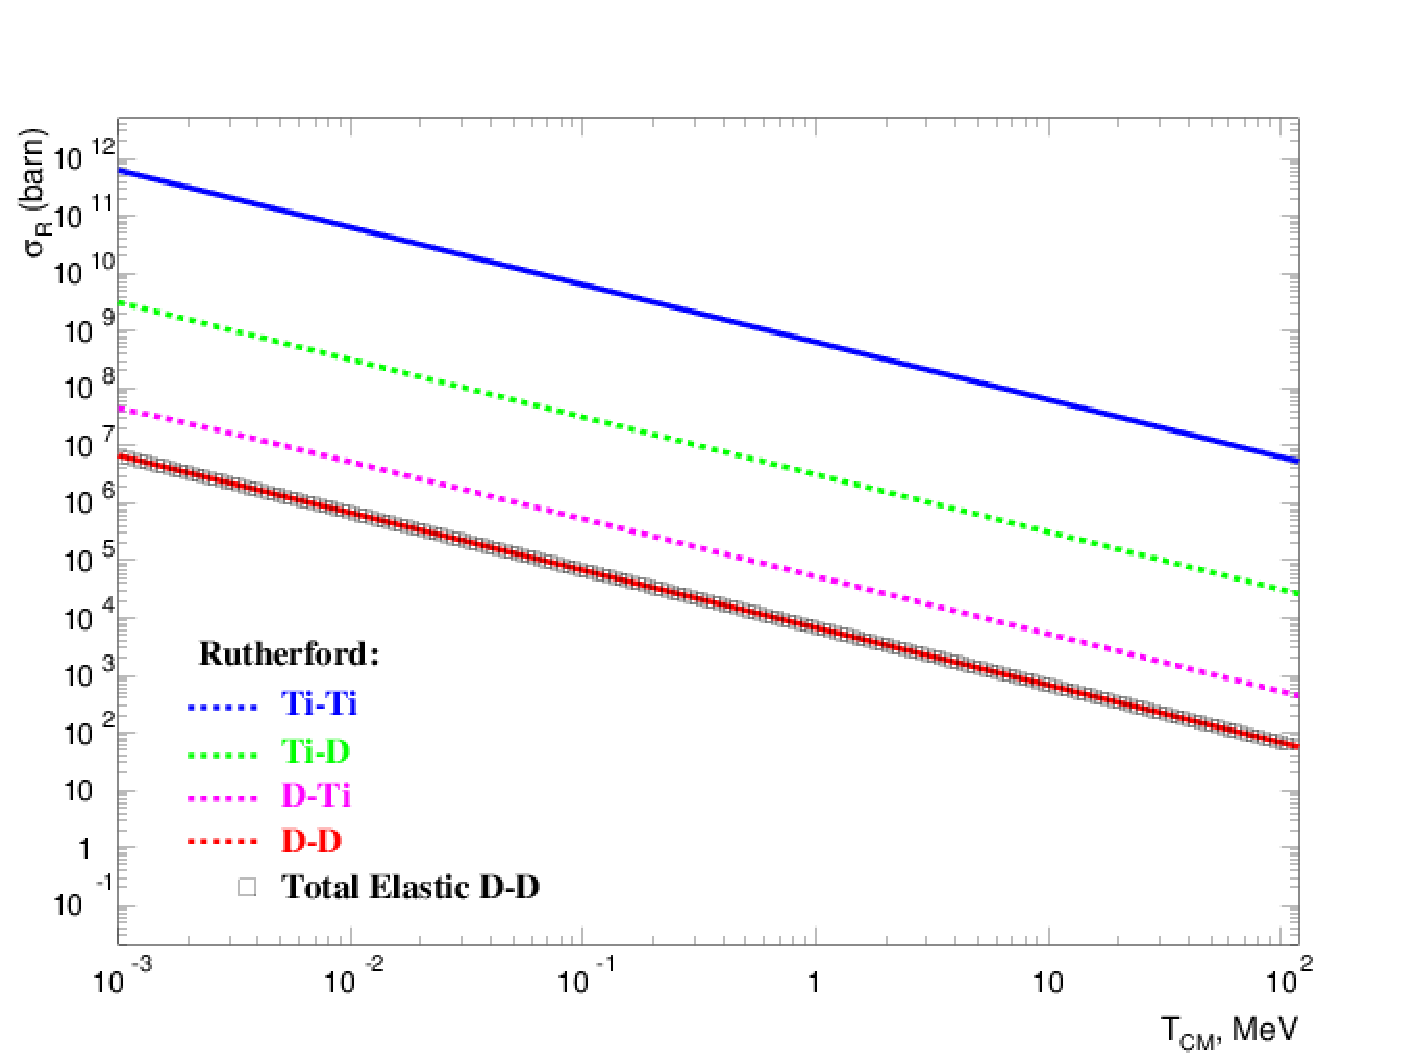
\includegraphics[width=0.99\linewidth]{images/integral_rutherford_d_ti_cross_sections.pdf}
  }
  \caption{Зависимости интегральных сечений D-D, D-Ti, Ti-D и Ti-Ti Резерфордовского рассеяния от кинетической энергии в системе центра масс $T_{CM}$. Пустыми квадратами показано интегральное сечение от аппроксимации экспериментальных данных дифференциального упругого сечения из базы ядерных данных EXFOR, осуществленной в отчёте [RepIonMat].}
  \label{fig:IntegralRutherfordDTiCrossSections}
\end{figure}

	Следует отметить, что при использовании аппроксимации дифференциального сечения упругого D-D рассеяния, полученной в отчёте [RepIonMat], интегральное сечение в итоге не отличается от интегрального сечения Резерфордовского рассеяния.
	Это связано с тем, что, как видно из Рис. ~    \ref{fig:DifferenceOfElasticDDFromRutherfordDifferentialCrossSection}, отличие полученной аппроксимации дифференциального сечения упругого D-D рассеяния наблюдается только при угле рассеяния, близком к $\frac{\pi}{2}$.
	Поэтому нетрудно заметить, что вклад этого отличия в итоговое интегральное сечение пренебрежимо мал, т. к. дифференциальное сечение упругого рассеяния сильно падает от 0 до $\frac{\pi}{2}$.
	
	Т. к. рассматриваемый процесс упругий, $p_{CM}$ не меняется до и после взаимодействия, самая большая сложность в реализации конечного состояния этого процесса (на вход подана 1 частица, на выходе получаются  2) будет в генерации случайного значения $\cos{\theta_{CM}}$.
	Ниже будет описано как проводился розыгрыш по случайному числу от 0 до 1 случайного значения $\cos{\theta_{CM}}$.
	
	Т. к. рассматривается задача моделирования ион-ионного каскада в дейтериде титана, то налетающая частица может рассеяться на ядрах только 2 типов: дибо ядрах дейтерия, либо изотопов титана.
	Т. к. при моделировании ионного каскада мишень из дейтерида титана облучается потоком дейтронов, то возможные варианты рассеяния: D-D, D-Ti, Ti-D, Ti-Ti.
	Таким образом, получается всего 2 варианта рассеяния: рассеяние различных частиц (D-Ti, Ti-D) и рассеяние тождественных частиц (D-D и Ti-Ti).
	
	Перед тем как приступать к осуществлению процесса рассеяния налетающей частицы, необходимо проверить условие $|t|_{min} \leq |t|_{max}$.
	Если оно выполнено, можно переходить к рассеянию частицы.
	Если же нет, т. е. $|t|_{max} \leq |t|_{min}$, то интегралы $\int \limits^{|t|_{max}}_{|t|_{min}} \frac{d\sigma_R}{d|t|} \cdot d|t|$ будут отрицательные, что не имеет смысла, поэтому следует вернуть значение $\cos{\theta_{CM}}=0$.
	Ситуация $|t|_{max}=4\cdot p^2_{CM} \leq |t|_{min}=2\cdot M \cdot E_{de}$ может возникнуть тогда, когда $p_{CM} \leq \sqrt{ \frac{1}{2} \cdot M \cdot E_{de} }$.
	Например, для D-D рассеяния эта ситуация возникает при $p_{CM} \leq 97$ кэВ, а для D-Ti -- при $p_{CM} \leq 1.5$ МэВ.
	
	При рассеянии различных частиц не возникает никаких затруднений: значение $|t|$ после рассеяния находится из соотношения $\int \limits^{|t|}_{|t|_{min}}=R \cdot \int \limits^{|t|_{max}}_{|t|_{min}} \frac{d\sigma_R}{d|t|} \cdot d|t|$, где $R$ -- псевдослучайное число от 0 до 1.
	При использовании (\ref{IntegralRutherfordCSDifferentParticles}) отсюда сразу получаются выражения
	
\begin{equation}
\label{TDifferentParticles}
\begin{aligned} 
   |t| = \frac{|t|_{min}}{1-R\cdot \left( 1-\frac{|t|_{min}}{|t|_{max}} \right)} 
\end{aligned}
\end{equation}

	и, т. к. $|t|=2\cdot p^2_{CM} \cdot \left( 1-\cos{\theta_{CM}} \right)$,
	
\begin{equation}
\label{CosThetCMDifferentParticles}
\begin{aligned} 
  \cos{ \theta_{CM}} = 1- \frac{|t|_{min}}{|t|_m \cdot \left( 1-R\cdot \left( 1-\frac{|t|_{min}}{|t|_{max}} \right) \right)},
\end{aligned}
\end{equation}

	где $|t|_{m}=2\cdot p^2_{CM}$ и $|t|_{max}=4\cdot p^2_{CM}$.
	
	Если рассеиваются одинаковые частицы, допустим Ti-Ti, D-D здесь не рассматривается, оно будет рассмотрено ниже, то, как видно из выражения (\ref{DifferentialRutherfordCSEqualParticles}), в дифференциальном сечении присутствуют 3 слагаемых, интеграл от каждого из которых от $|t|_{min}$ до $|t|_m=2\cdot p^2_{CM}$ (т. к. рассеиваются тождественные частицы, то максимальный угол рассеяния $\theta_{CM}=\frac{\pi}{2}$ и максимальное значение переменной $|t|$ равно $|t|_m=2\cdot p^2_{CM}$, а не $|t|_{max}=4\cdot p^2_{CM}$) должен рассматриваться отдельно.
	Т. е. как бы есть 3 ``канала'' рассеяния, с помощью случайного числа от 0 до 1 по соотношению интегралов происходит выбор, в каком канале рассеиваться, и по ещё одному случайному числу от 0 до 1 происходит рассеяние -- получается значение $|t|$ и $\cos{\theta_{CM}}$.
	
	Здесь возникает определённая сложность: интеграл от интерференционного члена в (\ref{IntegralRutherfordCSEqualDD}) может оказаться отрицательным, что вносит ошибку в определение того, какой канал выиграет.
	
	Чтобы этого не происходило, было принято решение определить величину $|t|_{mid}=\frac{|t|_{max}}{1+e^{\frac{\pi}{2} \cdot \frac{\beta^r_{CM}}{\alpha}}}$.
	Величина $|t|_{mid}$ определялаясь из условия того, чтобы фаза синуса в интеграле от интерференционного слагаемого в (\ref{IntegralRutherfordCSEqualParticles}) была меньше $\frac{\pi}{2}$, т. е. чтобы интеграл от интерференционного слагаемого не становился отрицательным.
	Таким образом, получалось, что при $|t| > |t|_{mid}$ интеграл от интерференционного члена в дифференциальном сечении был неотрицательным.
	
	Определение того, какой ``канал'' Резерфордовского рассеяния тождественных частиц выиграет, происходило следующим образом.
	Вычислялись интегралы от 1-го и 2-го членов: $I_1=I_2=\frac{\pi}{p^2_{CM}} \cdot \left( m \alpha \hbar c Z^2 \right)^2 \cdot \left( \frac{1}{|t|_{min}} - \frac{1}{|t|_{max}-|t|_{min}} \right)$, т. к. частицы тождественные, то $m=M$ и $z=Z$.
	Интеграл от интерференционного члена в дифференицальном сечении (\ref{DifferentialRutherfordCSEqualParticles}) определялся как интеграл от $|t|_{mid}$ до $|t|_{max}$.
	Если $|t|_{mid} > |t|_{max}$, он был равен нулю.
	Если же $|t|_{mid} < |t|_{min}$, то он считался от $|t|_{min}$ до $|t|_{max}$.
	С помощью равномерно распределённого случайного числа от 0 до 1 определялось, по какому каналу будет происходить генерация случайных $|t|$ и $\cos{\theta_{CM}}$.
	
	Если выигрывал 1-ый канал, то $|t|$ определялось как
	
\begin{equation}
\label{Channel1TEqualParticles}
\begin{aligned} 
  |t| = \frac{1}{ \frac{1-R}{|t|_{min}} + \frac{R}{|t|_m} },
\end{aligned}
\end{equation}

	если 2-ой, то как
	
\begin{equation}
\label{Channel2TEqualParticles}
\begin{aligned} 
  |t| = |t|_{max} - \frac{1}{ \frac{1-R}{|t|_{max}-|t|_{min}} + \frac{R}{|t|_m} },
\end{aligned}
\end{equation}

	а если 3-ий, то как
	
\begin{equation}
\label{Channel3TEqualParticles}
\begin{aligned} 
  |t| = \frac{ |t|_{max} \cdot e^A}{1+e^A},
\end{aligned}
\end{equation}

	где
	
\begin{equation}
\label{Channel3TEqualParticlesA}
\begin{aligned} 
  A = \frac{ \beta^r_{CM} }{\alpha} \cdot \arcsin{ \left( \sin{ \frac{\alpha}{\beta^r_{CM}} \cdot \ln{ \frac{|t|_{min}}{|t|_{max}-|t|_{min}} } } \cdot \left( 1-R \right) \right) }.
\end{aligned}
\end{equation}

	Здесь $R$ -- равномерно распределённое случайное число от 0 до 1, а $|t|$ разыгрывается от $|t|_{min}$ не до $|t|_{max}=4\cdot p^2_{CM}$, а до $|t|_m=2\cdot p^2_{CM}$, т. е. не до $\theta_{CM}=\pi$, а до $\theta_{CM}=\frac{\pi}{2}$, потому что рассеиваются тождественные частицы.
	
	Далее, из полученного сгенерированного случайного значения $|t|$ получалось значение $\cos{ \theta_{CM} }=1-\frac{|t|}{2\cdot p^2_{CM}}$.
	
	При моделировании упругого D-D расеяния ситуация была несколько сложнее.
	Как упоминалось в разделе \ref{ValElasticDD}, в отчёте [RepIonMat] была получена аппроксимация упругого дифференциального сечения D-D рассеяния, отличающаяся от Резерфордовского дифференциального сечения только при максимальных углах рассеяния в системе центра масс, близких к $\frac{\pi}{2}$.
	Она изображена на Рис. ~\ref{fig:DifferenceOfElasticDDFromRutherfordDifferentialCrossSection} в дважды логарифмическом масштабе, где по оси абсцисс отложена безразмерная переменная $1-\cos{ \theta_{CM}}$.
	
	
\begin{figure}[ht]
  {
     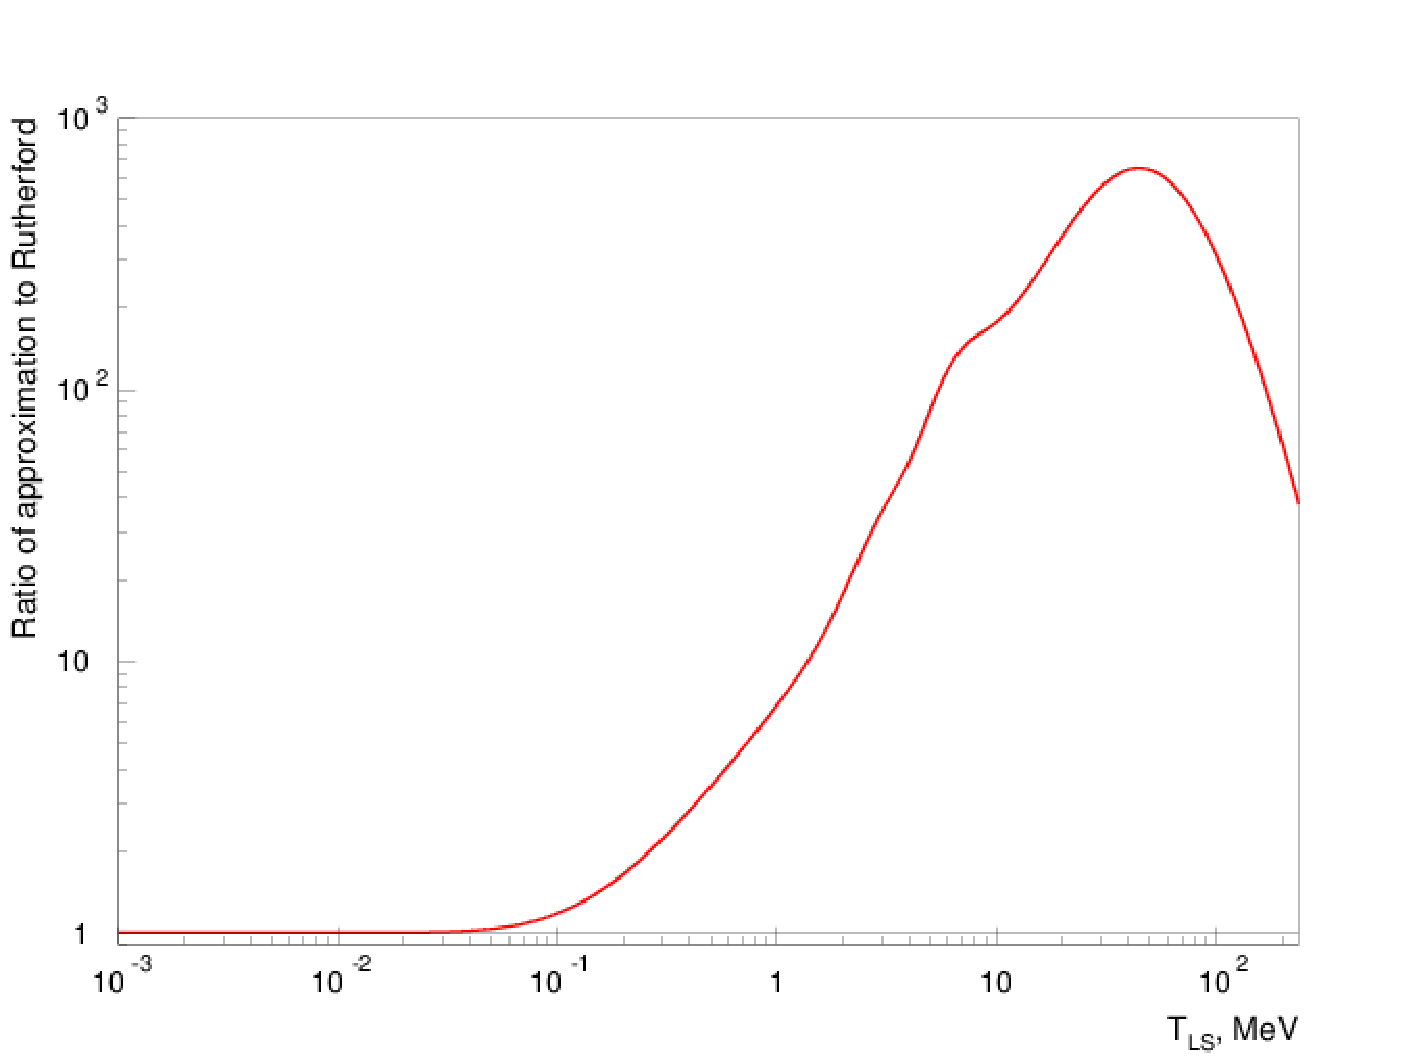
\includegraphics[width=0.5\linewidth]{images/ratio_of_elastic_dd_at_90_grades.pdf}
     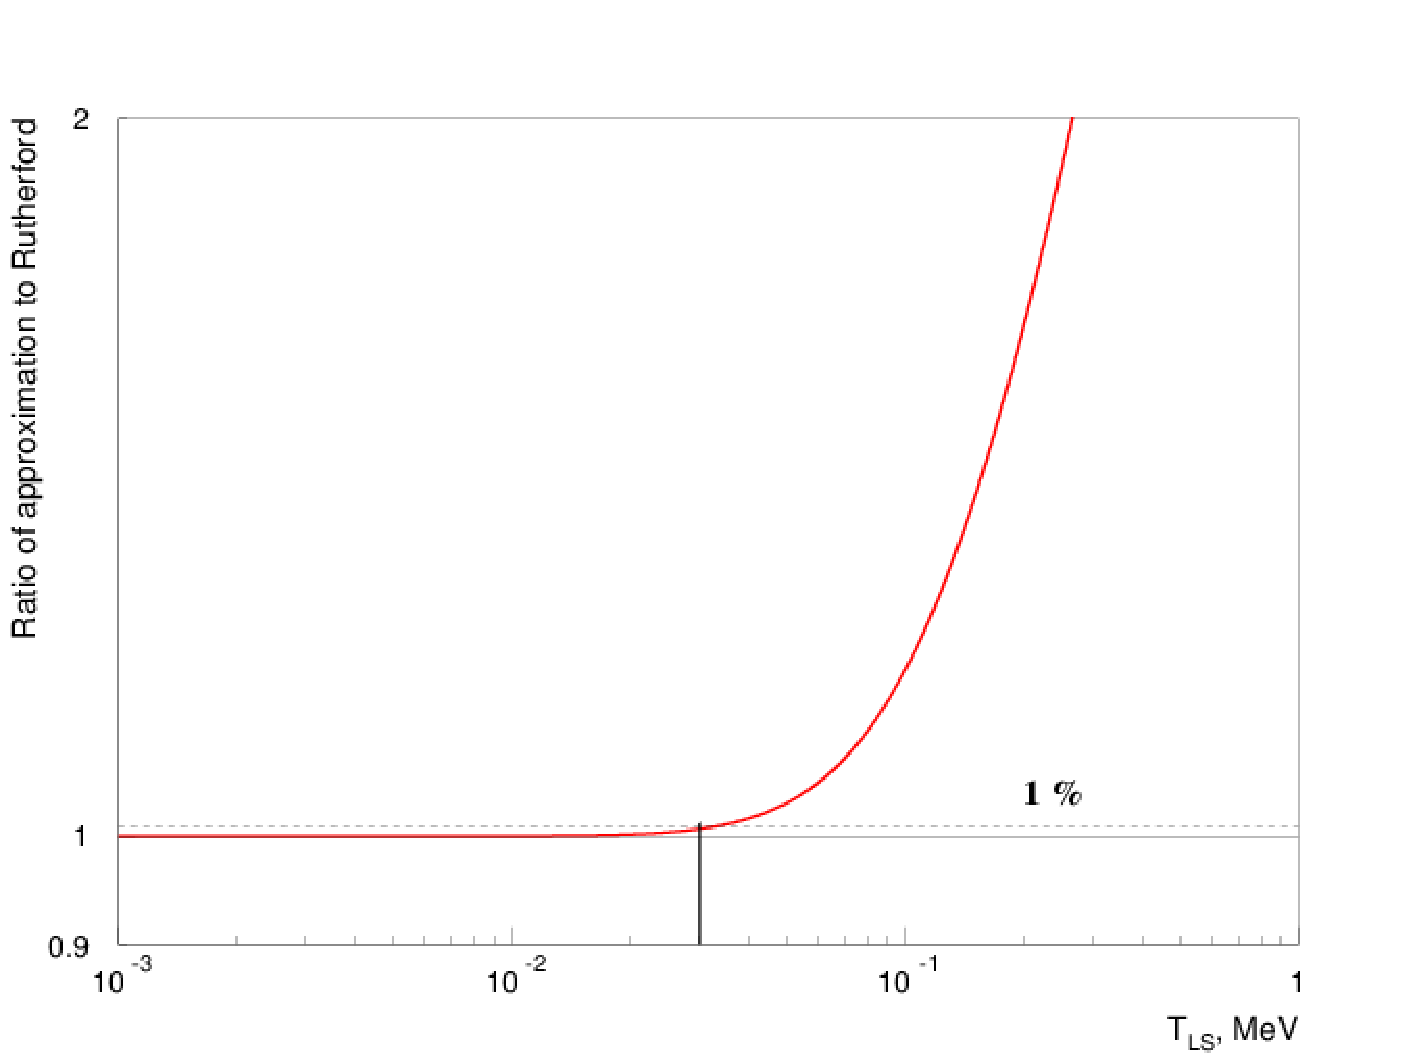
\includegraphics[width=0.5\linewidth]{images/ratio_of_elastic_dd_at_90_grades_find_1_percent_diff.pdf}
  }
  \caption{\textit{\textbf{Слева:}} Отношение полученной в отчёте [RepIonMat] и изображённой на Рис. ~\ref{fig:DifferenceOfElasticDDFromRutherfordDifferentialCrossSection} аппроксимации дифференциального сечения упругого D-D рассеяния при угле рассеяния $\theta_{CM}=\frac{\pi}{2}$ к значению дифференциального сечения Резерфордовского рассеяния при $\theta_{CM}=\frac{\pi}{2}$ при одной и той же кинетической энергии налетающего дейтрона $T_{LS}$.
  \textit{\textbf{Справа:}} То же отношение, увеличенное в области, где оно только начинает отличаться от 1 так, чтобы можно было видеть начиная с какой $T_{LS}$ отличие составляет не менее 1 \%.}
  \label{fig:RatioOfElasticDDAt90Grades}
\end{figure}	
	
	
	Как хорошо видно из Рис. ~\ref{fig:RatioOfElasticDDAt90Grades}, при $T_{LS} \leq 10$ кэВ полученная аппроксимация никак не отличается от дифференциального Резерфордовского сечения.
	
	В то же время, необходимо было выяснить, где при $T_{LS}>10$ кэВ аппроксимация совпадает с дифференциальным Резерфордовским сечением , а где от него отличается. 
	При взгляде на Рис. ~\ref{fig:DifferenceOfElasticDDFromRutherfordDifferentialCrossSection} затруднительно сразу ответить на этот вопрос. 
	Было проведено исследование, в ходе которого для каждого из значений $T_{LS}$ на Рис. ~\ref{fig:DifferenceOfElasticDDFromRutherfordDifferentialCrossSection} было найдено, начиная с какого значения $1-\cos{ \theta_{CM} }$ между аппроксимацией и дифференциальным Резерфордовским сечением имеется не менее чем 10 \% отличие. 
	Было выяснено, что полученные для каждого из значений $T_{LS}$ на Рис. ~\ref{fig:DifferenceOfElasticDDFromRutherfordDifferentialCrossSection} величины $1-\cos{ \theta_{CM} }$, начиная с которых отличие аппроксимации от Резерфордовского дифференциального сечения составляет не менее 10 \%, группируются вокруг значения $10^{-3}$. 
	Так что с неплохой точностью можно считать, что при любых $T_{LS}$ в рассматриваемом диапазоне $10$ кэВ $\leq T_{LS} \leq 250$ МэВ (самая большая кинетическая энергия налетающего дейтрона $T_{LS}$ в экспериментальных данных, использовавшихся  для аппроксимации, равняется 231.8 МэВ, поэтому мы приближённо считаем, что верхняя граница применимости полученной аппроксимации по $T_{LS}$ равна 250 МэВ) упругого D-D рассеяния при $1-\cos{ \theta_{CM}} < 10^{-3}$ нет никакого отличия между полученной аппроксимацией и Резерфордовским дифференциальным сечением D-D рассеяния, а при $1-\cos{ \theta_{CM}} \geq 10^{-3}$ чем ближе к $\theta_{CM}=\frac{\pi}{2}$, тем больше отличие аппроксимации от дифференциального сечения рассеяния Резерфорда и поэтому, для того чтобы точнее описывать угловое распределение D-D упругого рассеяния, нужно использовать полученную аппроксимацию.
	
	Поэтому упругое D-D рассеяние описывалось следующим образом.
	Если кинетическая энергия налетающего дейтрона $T_{LS}$ была меньше 10 кэВ, считалось, что в этой области есть только Резерфордовское дифференциальное сечение рассеяния тождественных частиц, и случайный $\cos{\theta_{CM}}$ генерировался как только что было описано выше.
	Если же $T_{LS}$ была больше 10 кэВ, то в рамках процесса упругого ион-ионного рассеяния интегральное сечение упругого D-D рассеяния вычислялось как интеграл от Резерфордовского дифференциального сечения рассеяния тождественных частиц от $|t|_{min}$ до $10^{-3}\cdot |t|_{m}=2\cdot 10^{-3}\cdot p^2_{CM}$.
	Аналогично, и случайное значение $|t|$ разыгрывалось от $|t|_{min}$ до $10^{-3}\cdot |t|_m$.
	
	Область $10^{-3} \cdot |t|_m \leq |t|_m$ для упругого D-D рассеяния разыгрывалась в отдельном процессе упругого D-D рассеяния, который будет описан в следующем разделе.
	
	Применительно к задаче моделирования ионного каскада в мишени из дейтерида титана, вызванной облучением мишени потоком дейтронов, на вход рассматриваемому процессу подавался вектор 4-импульса налетающего иоа, а на выходе получался рассеянный налетающий ион, и ядро отдачи.


\subsection{Реализация дискретного процесса упругого D-D рассеяния.}
\label{ElasticDDScatteringRealization}

	Процесс упругого D-D рассеяния в области $T_{LS} \geq 10$ кэВ реализовывался при использовании аппроксимации дифференциального сечения упругого D-D рассеяния, полученной в [RepIonMat].
	
	В области $10^{-3} \leq 1-\cos{\theta_{CM}} \leq 1$ слева направо задавалась логарифмическая шкала оси абсцисс и справа налево проводилось интегрирование $\int \limits^{|t|_m}_{10^{-3}\cdot |t|_m} \frac{d\sigma^{approx}}{d|t|} \cdot d|t|$.
	Т. к. $\frac{d\sigma^{approx}}{d|t|} \sim \frac{1}{|t|^2}$, поэтому интегрирование проводилось справа налево, чтобы учесть малый вклад правых логарифмических бинов.
	Ведь если проводить интегрирование слева направо, в самых правых логарифмических бинах, где величина значений функции на порядки меньше её значений в самых левых бина, значения нормированных частичных сумм будут чень мало отличаться от 1 и друг от друга.
	Интегрирование справа налево позволяет избавиться от этой проблемы.
	
	Интегральные сечения данного процесса определялись как $2 \cdot \int \limits^{|t|_m}_{10^{-3}\cdot |t|_m} \frac{d\sigma^{approx}}{d|t|} \cdot d|t|$, т. к. рассеиваются тождественные частицы, а значит, дифференциальное сечение рассеяния симметрично относительно угла рассеяния $\theta_{CM}=\frac{\pi}{2}$.
	Так же в ходе интегрирования были получены частичные суммы, соответствующие интегралам $\int \limits^{|t|_m}_{|t|_i} \frac{d\sigma^{approx}}{d|t|} \cdot d|t|$, где $|t|_i$ -- левые границы логарифмических бинов, а $i=0..N_{bin}-1$, $N_{bin}$ -- число бинов, равное 128, которые делились на полный интеграл от $|t|_{min}$ до $10^{-3} \cdot |t|_m$, в результате чего для каждой из 100 значений $T_{LS}$ в диапазоне 10 кэВ $\leq$ 250 МэВ получался набор данных ($1-cos{\theta_{CM}}$, частичные суммы).
	
	Розыгрыш случайного значения $\cos{\theta_{CM}}$ проводился следующим образом.
	Сначала по значению $T_{LS}$ налетающего дейтрона при использовании бинарного поиска определялись 2 соседних набора частичных сумм, соответствующие значениям $T_{LS}$, между которыми находится $T_{LS}$ налетающего дейтрона.
	Далее, с помощью равномерно распределённого случайного числа от 0 до 1 и квадратичной интерполяции определялось значение $\cos{\theta_{CM}}$.
	
	На вход данному процессу подавался вектор 4-импульса налетающего дейтрона, а на выходе получались 2 4-импульса -- рассеянного дейтрона и дейтрона отдачи.
	Если налетающая частица не была дейтроном, интегральное сечение процесса было равно 0, и процесс упругого рассеяния не осуществлялся.
	
	
\subsection{Неперывные процессы многократного рассеяния и $\frac{dE}{dx}$.}
\label{MSanddEdxRealization}

	Также в ходе моделирования присутствовали непрерывные (которые происходят не дискретно в вершине взаимодействия, а непрерывно вдоль трека частицы) многократного рассеяния и линейных электронных потерь энергии частицы в материале мишени $\frac{dE}{dx}$.
	
	Непрерывный процесс многократного рассеяния подробно описан в разделе \ref{ValMS}.
	Он приводит к изменению на каждом шаге моделирования направления вектора импульса каждой заряженной частицы, проходящей через материал мишени на некий малый угол, величина которого определялась аппроксимацией функции плотности вероятности углового распределения многократного рассеяния (\ref{MSApproximationFunction}) при должном скейлинге, описанном в разделе \ref{subValMS2}.
	
	Непрерывный процесс линейных электронных потерь энергии заряженной частицы на каждом шаге моделирования подробно описан в разделе \ref{ValdEdx}.
	Он просто приводит к уменьшению энергии каждой заряженной частицы на шаге в соответствии с $E=E-\frac{dE}{dx} \cdot l$, где $l$ -- пробег частицы на шаге.

	
\clearpage{}
\section{Моделирование выхода нейтронов при облучении мишени из дейтерида титана интенсивным потоком дейтронов.}
\label{NeutronOutput}

	Перед моделированием ионного каскада в мишени из дейтерида титана необходимо было удостовериться, что в результате облучения мишени из дейтерида титана интенсивным потоком дейтронов с начальной кинетической энергией 100 кэВ правильным образом -- с согласующейся с результатами экспериментов вероятностью -- генерируются нейтроны в результате реакции неупругого D-D рассеяния.
	
	Т. к. для моделирования выхода нейтронов интересны только дейтроны, то все вторичные частицы, получающиеся в ходе процессов непругой D-D реакции и упругого ион-ионного рассеяния: протоны, тритоны, ядра $^3_2$He и изотопов титана считались и исключались из моделирования.
	Нейтроны тоже подсчитывались и исключались из моделирования.  

\subsection{Пробег дейтронов в дейтериде титана в зависимости от энергии остановки дейтерия.}
\label{DeuteronRangesInTiD2}
	
	Для ускорения моделирования, а, главным образом, потому что сечение неупругой D-D реакции меделенных дейтронов быстро падает суменьшением энергии, и ожидать выхода нейтронов с $T_{LS} \leq 10-20$ кэВ бессмысленно, при $T_{LS} \leq 10$ кэВ дейтроны исключались из моделирования.
	
	Для того чтобы знать толщину мишени, на которой все дейтроны, запущенные с энергией 100 кэВ, гарантированно остановятся, необходимо было подсчитать длину пробега дейтронов материале мишени, равную $\int \limits^{T^{max}_{LS}}_{T^{min}_{LS}} \frac{dx}{dE} \cdot dE$, где использовалась полученная аппроксимация $\frac{dE}{dx}$ для протонов в дейтериде титана и скейлинг, описанные в разделе \ref{ValdEdx}, и $T^{max}_{LS}=100$ кэВ, а $T^{min}_{LS}=10$ кэВ. В результате численного интегрирования было получено значение 0.865 мкм.
	
	Было интересно посмотреть, как зависит длина пробега от ``энергии обрезания'' $T_{CUT}$, которая была положена равной 10 кэВ.
	Если изменять величину $T_{CUT}$, то получающаяся зависимость длины пробега дейтронов в мишени из дейтерида титана от $T_{CUT}$ показана на Рис. ~\ref{fig:RangesOfDeuteronsInTiD2}.
	  
\begin{figure}[ht]
  {
     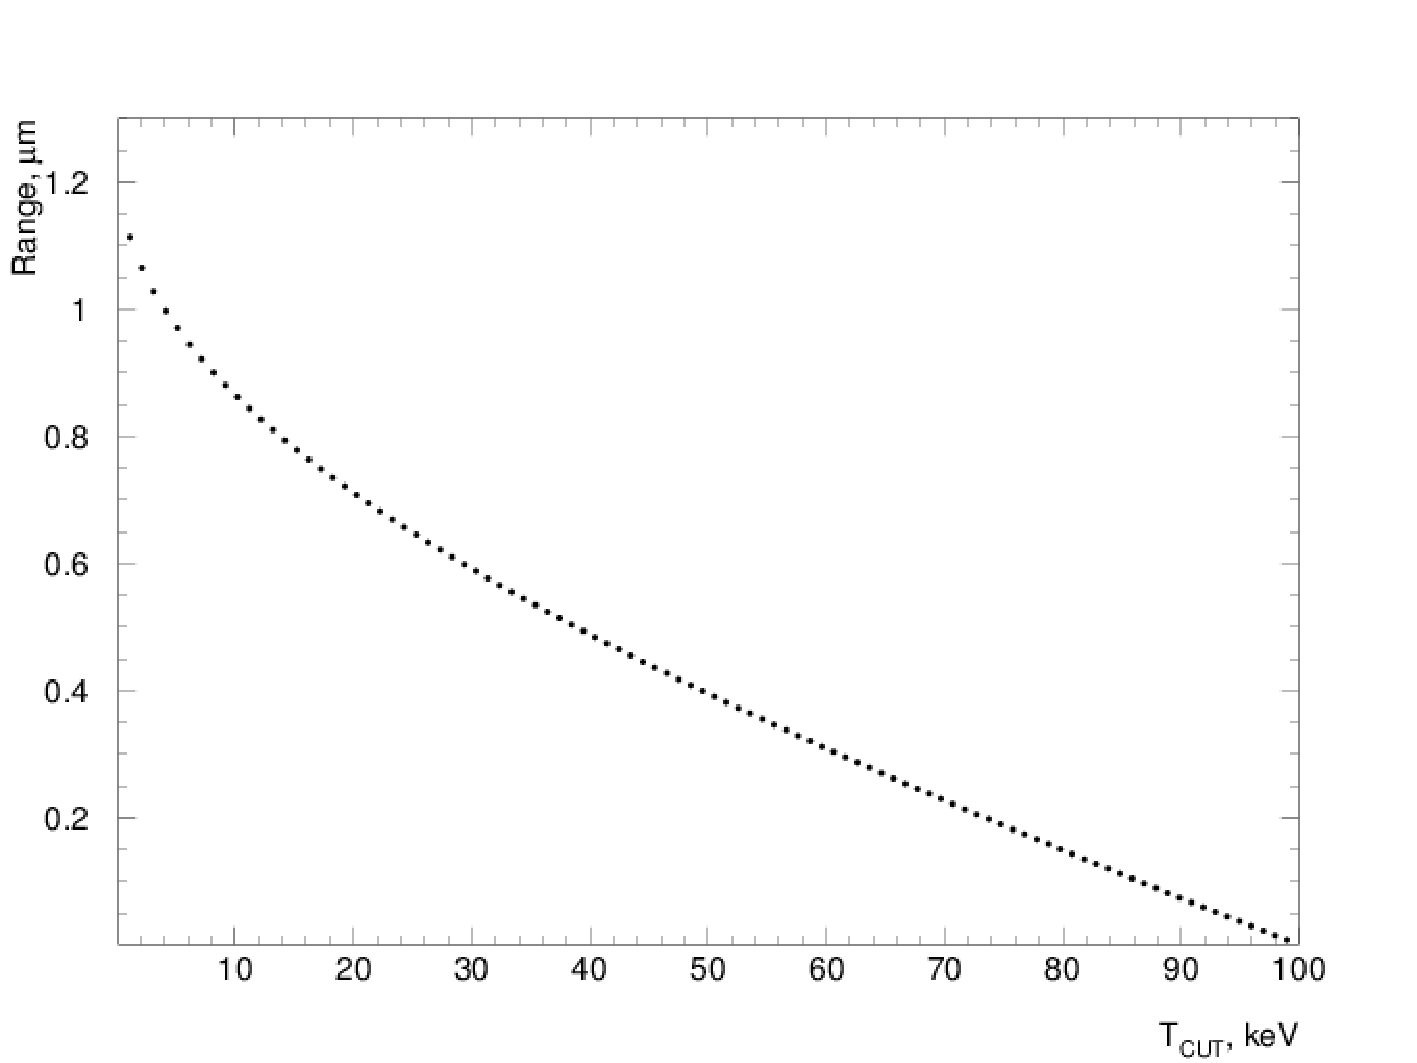
\includegraphics[width=0.99\linewidth]{images/ranges.pdf}
  }
  \caption{Зависимость длины пробега дейтронов с начальной кинетической энергией 100 кэВ в мишени из дейтерида титана от значения кинетической энергии обрезания $T_{CUT}$.}
  \label{fig:RangesOfDeuteronsInTiD2}
\end{figure}

\subsection{Средние пробеги дейтронов в дейтериде титана в зависимости от кинетической энергии.}
\label{DeuteronMeanRangesDependenceOnEnergyInTiD2}

	С целью узнать зависимость средних пробегов дейтронов в процессах упругого ион-ионного рассеяния и реакции неупругого D-D рассеяния было произведено моделирование, в результате которого были получены гистограммы распределения средних длин пробега дейтронов в данных процессах в зависимости от их кинетической энергии.
	Они изображены на Рис. ~\ref{fig:RangesOfDeuteronsInInelasticAndElasticProcesses}.
	При составлении данных гистограмм оставлялся включенным только интересующий процесс, сечения остальных процессов фиктивно ставились равными 0.  
	
\begin{figure}[ht]
  {
     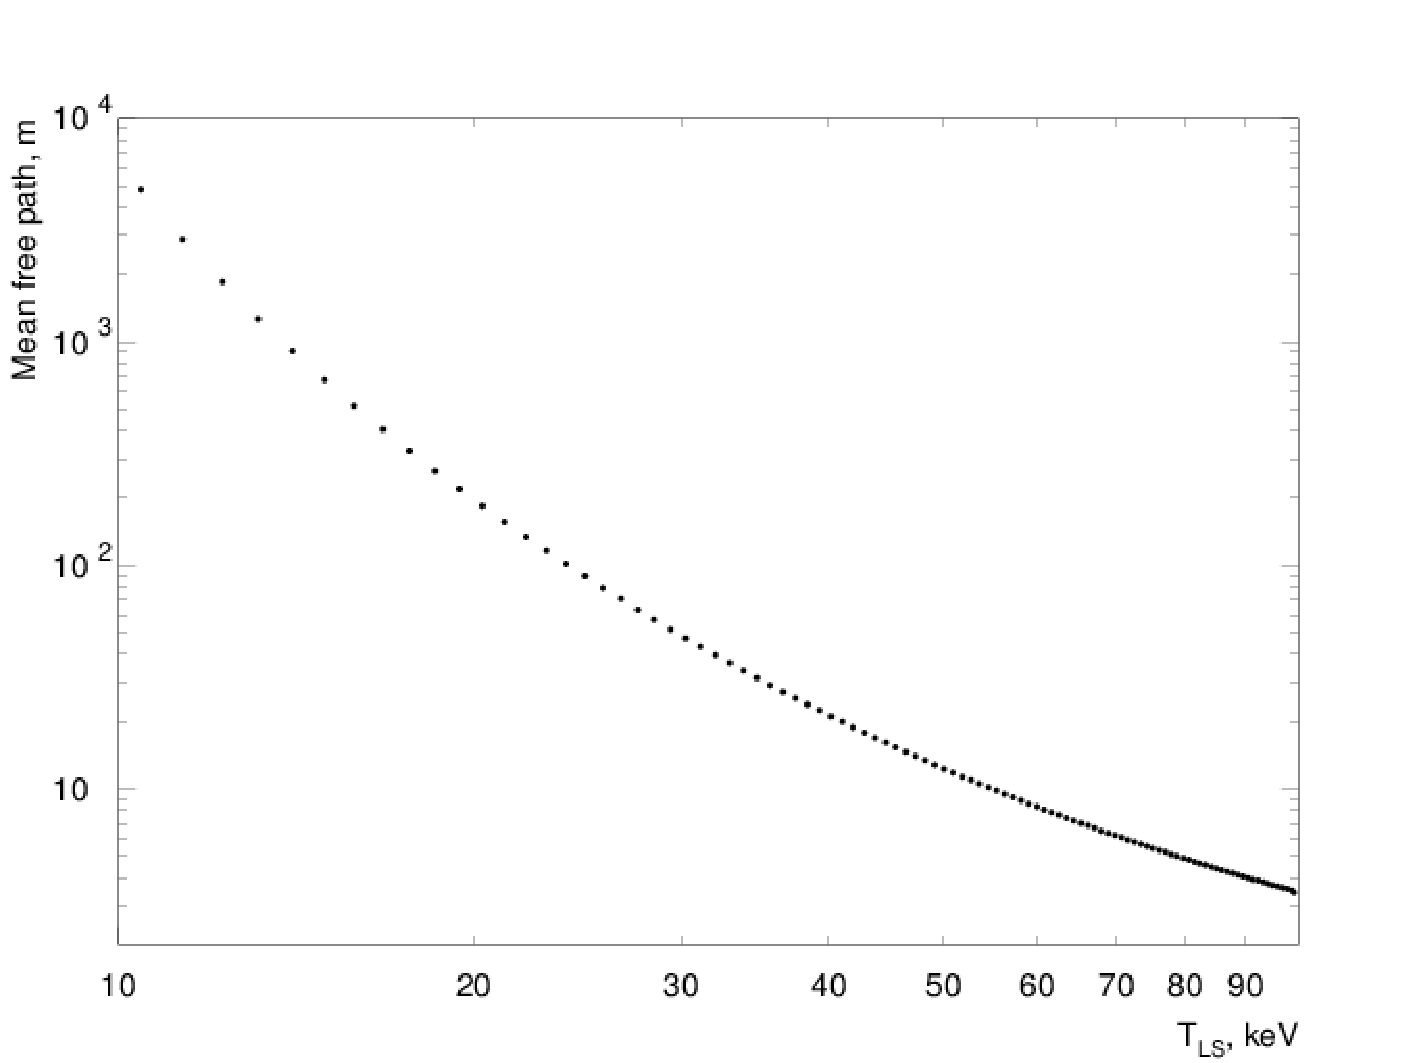
\includegraphics[width=0.5\linewidth]{images/fluence_inelastic.pdf}
     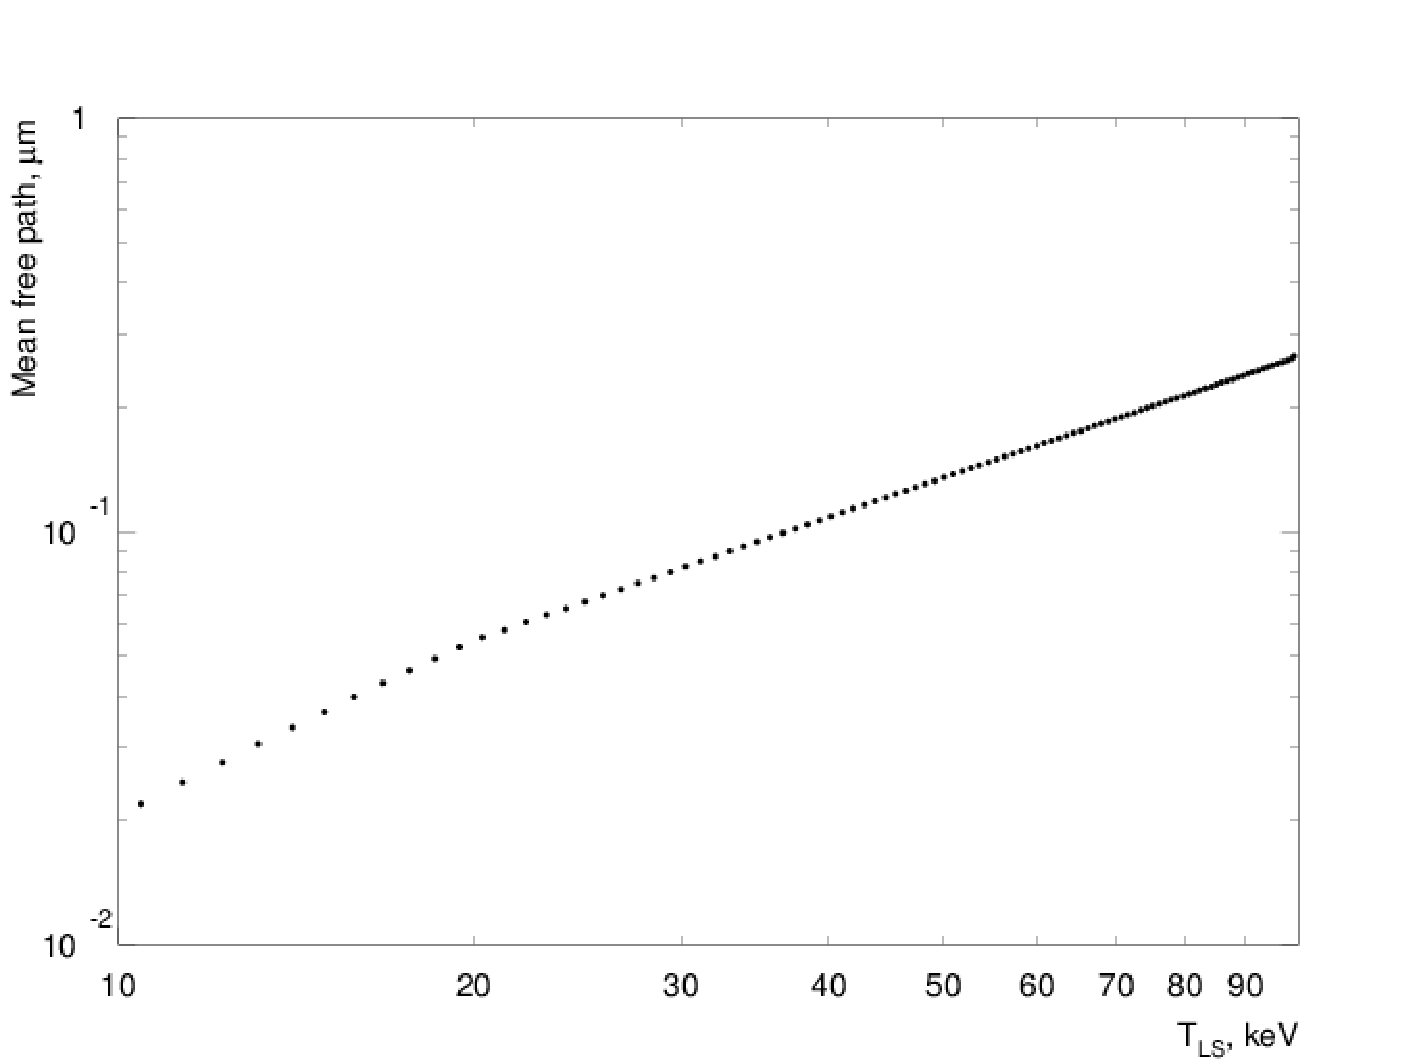
\includegraphics[width=0.5\linewidth]{images/fluence_elastic.pdf}
  }
  \caption{Зависимость средней длины свободного пробега дейтронов в дейтериде титана в зависимости от их кинетической энергии в процессах: \textbf{\textit{слева}} -- реакции неупругого D-D рассеяния, \textbf{\textit{справа}} -- упругого ион-ионного рассеяния.}
  \label{fig:RangesOfDeuteronsInInelasticAndElasticProcesses}
\end{figure}
	
\subsection{Вероятность нейтронного выхода на 1 запущенный дейтрон.}
\label{ProbabilityOfNeutronOutputPer1Deuteron}

	Зная распределение средних длин свободного пробега в полноценном процессе моделирования, когда включены и все процессы -- и неупругая D-D реакция, и упругое ион-ионное рассеяние -- можно узнать вероятность нейтронного выхода на 1 запущенный дейтрон.
	
	Для этого нужно из получившегося распределения средних длин свободного пробега дейтронов в зависимости от их кинетической энергии посчитать величину $\frac{dl}{dE}$  и свернуть её с $n_{TiD_2} \cdot \sigma_{Inelastic\,DD}$. Это было сделано, в результате чего была получена вероятность нейтронного выхода на 1 запущенный дейтрон:
	
\begin{equation}
\label{ProbabilityOfNeutronOutputPer1Deuteron}
\begin{aligned} 
  P = \int \limits^{T^{max}_{LS}}_{T^{min}_{LS}} \frac{dl}{dE} \cdot n_{TiD_2} \cdot \sigma_{Inelastic\,DD} \cdot dE = 2.7 \cdot 10^{-8}.
\end{aligned}
\end{equation}

\subsection{Нейтронный выход в ходе моделирования.}
\label{NeutronOutputInModelling}

	В результате моделирования нейтронного выхода от $N_D$ запущенных дейтронов был получен следующий результат:
	
\begin{tabular}{|c|c|c|}
 \hline 
 $N_D$ & Общее число непругих D-D реакций & Выход нейтронов \\ 
 \hline 
 $10^6$ & 0 & 0 \\ 
 \hline 
 $10^7$ & 2 & 2 \\ 
 \hline 
 $10^8$ & 12 & 4 \\ 
 \hline 
 $10^9$ & 153 & 72 \\ 
 \hline 
 \end{tabular}
 
 
 
	 
	
	
	





	
	
	
  При $|t|>|t|_{min}$ можно рассматривать полное дифференциальное сечение упругого рассеяния, являющееся интерференцией электромагнитной (Резерфордовской) и ядерной амплитуд рассеяния.
  При этом, так как Резерфордовское дифференциальное сечение рассеяния различных частиц, определяющееся выражением (\ref{Dimension1p}), неограниченно растёт при $|t| \to 0$, для того, чтобы полное сечение, являющееся интегралом от дифференциального сечения, сходилось, необходимо учитывать постоянную электронной экранировки $A_S$, делающую $\frac{d\sigma}{d|t|}$ конечным при $|t| \to 0$ ($\theta_{CM} \to 0$, $\theta_{LS} \to 0$):
\begin{equation}
 \begin{aligned} 
 \label{MS1}     
      \frac{d\sigma}{d|t|}=  
      \frac{A_R^2}{\left( |t| + 4 p_{CM}^2 A_S \right)^2} \cdot \left( \hbar c \right)^2,
 \end{aligned}
\end{equation}
где согласно \cite{G4IonIon}:
\begin{equation}
\label{MSAs}
\begin{aligned} 
A_S= \left( \frac{ \hbar }{ 2 p_{CM} a_L } \right)^2 \cdot \left( 1.13 + 3.76 \cdot \left( \frac{ \alpha z Z}{\beta_{CM}} \right)^2 \right).
\end{aligned}
\end{equation}

Здесь $p_{CM}$ -- импульс в системе центра масс, радиус электронной экранировки определяется выражением, рассчитанным в \cite{LinhardScreeningLength}:
\begin{equation}
\label{MSaL}
\begin{aligned} 
a_L=\frac{ C_{TF} \cdot a_0 }{ \left( z^{2/3} + Z^{2/3} \right) },
\end{aligned}
\end{equation} 
где $C_{TF}= \frac{1}{2} \left( \frac{3\pi}{4} \right)^{2/3}$ -- постоянная электронной экранировки Томаса-Ферми \cite{ThomasFermiModel}, $a_0=\frac{ \hbar^2 }{ m_ee^2 }$ -- боровский радиус, $m_e$ -- масса электрона, $z$ и $Z$ -- заряды налетающей частицы и мишени, $\beta_{CM}=\frac{p_{CM}}{E_{CM}^{\mu}}$ -- скорость приведённой частицы в системе центра масс ($c=1$), а энергия приведённой частицы в системе центра масс $E_{CM}^{\mu}=\sqrt{p_{CM}^2+\mu^2}$, где приведённая масса $\mu=\frac{mM}{m+M}$ и $m$ -- масса покоя налетающей частицы, $M$ -- масса покоя ядра-мишени.

Прежде чем перейти к вычислению сечения многократного рассеяния, необходимо упомянуть, что переменная $|t|$ ограничена сверху значением (\ref{Tmax}),
соответствующим рассеянию в системе центра масс на максимальный угол $\theta_{CM}=\pi$ (см. (\ref{Xp})). Тогда верхний предел интегрирования выражения (\ref{MS1}), необходимый для вычисления интегрального сечения многократного рассеяния, можно определить как величину $|t|_m$, равную $|t|_m=|t|_{max}$, если $|t|_{max}<|t|_{min}$, и $|t|_m=|t|_{min}$, если $|t|_{max} \geq |t|_{min}$.

Сечение многократного рассеяния в переднюю полусферу можно тогда определить как
\begin{equation}
\label{MSSigmaFull} 
\sigma^*_{ms}= \int \limits_0^{|t_{m}|} \frac{\left( \hbar c \right)^2 A_R^2 d|t|}{\left( |t| + 4p_{CM}^2 A_S \right)^2} = \left( \frac{\mu \alpha z Z \hbar c }{2p_{CM}^2} \right)^2 \frac{\pi\frac{|t_{m}|}{p_{CM}^2}}{ A_S \left( \frac{|t_{m}|}{4p_{CM}^2} + A_S \right) }.
\end{equation}

Выражение (\ref{MSSigmaFull}) справедливо для рассеяния различных частиц ($D-Ti$, $Ti-D$ и т. п.). В случае рассеяния тождественных частиц ($p-p$, $D-D$, $Ti-Ti$ и т. п.), когда дифференциальное сечение $\frac{d\sigma}{d|t|}$ симметрично относительно $|t|=2p_{CM}^2$, соответствующего углу рассеяния в системе центра масс $\frac{\pi}{2}$, формула (\ref{MSSigmaFull}) принимает вид
\begin{multline}
\label{MSSigmaFullEqual}
%\begin{aligned} 
\sigma_{ms}= \left( \hbar c \right)^2  A_R^2 \left( \int \limits_0^{|t_{m}|} \frac{d|t|}{\left( |t| + 4p_{CM}^2 A_S \right)^2} + \int \limits_{|t_{max}|-|t_m|}^{|t_{max}|} \frac{d|t|}{\left( |t| + 4p_{CM}^2 A_S \right)^2} \right)= \\ \left( \frac{\mu \alpha z Z \hbar c }{2p_{CM}^2} \right)^2 \frac{2\pi\frac{|t_{m}|}{p_{CM}^2}}{ A_S \left( \frac{|t|_{m}}{4p_{CM}^2} + A_S \right)} = 2 \sigma^*_{ms}.
%\end{aligned}
\end{multline}

  В процессе моделирования при использовании формулы (\ref{MSSigmaFull}) для описания сечения многократного рассеяния дейтрона на ядре титана и (\ref{MSSigmaFullEqual}) -- дейтрона на дейтроне, вычислялось среднее сечение многократного рассеяния дейтронов на одном рассеивающем центре (отдельной молекуле TiD$_2$).
  Плотность дейтерида титана $\rho_{TiD_2}=3.91$ г/см$^3$. Молекула TiD$_2$ состоит из 3 атомов: 2 атомов дейтерия и 1 атома $^{48}Ti$, соответственно доля элементов в дейтериде титана -- $\frac{2}{3}$ для дейтерия и $\frac{1}{3}$ для титана.
  В итоге среднее сечение на одном рассеивающем центре вычислялось как $\sigma_{av}=\frac{2}{3}\sigma_D^{in} +\frac{1}{3}\sigma_{Ti}^{in}$, где $\sigma_{D/Ti}^{in}$ -- интегральное сечение рассеяния налетающего ``in'') дейтрона с заданной энергией на ядре дейтерия/титана, находящемся в узле кристаллической решётки.
  Концентрация всех ядер в дейтериде титана находилась как $n_{TiD_2}=\frac{\rho_{TiD_2}}{\frac{2}{3}m_D +\frac{1}{3}m_{Ti}}=1.36 \cdot 10^{23}$ см$^{-3}$, где $m_{D/Ti}$ -- массы покоя ядер дейтерия/титана, равные 1875.6 МэВ и 44652 МэВ соответственно.
  Для перевода плотности из единиц г/см$^3$ в МэВ/см$^3$ использовался коэффициент пересчёта 1 г = 5.6096$\cdot 10^{26}$ МэВ.

По среднему сечению многократного рассеяния на одном ядре $\sigma_{av}$ и по концентрации всех ядер в дейтериде титана $n_{TiD_2}$ находилась средняя длина свободного пробега дейтрона в TiD$_2$:
\begin{equation}
\label{MSMeanFreePath}
\begin{aligned} 
<\lambda>= \frac{1}{n_{TiD_2} \sigma_{av}}.
\end{aligned}
\end{equation}  
Реальная же длина свободного пробега данной частицы на данной итерации вычислялась как
$\lambda=<\lambda> |\ln{R_1}|$, где $R_1$ -- псевдослучайное число от 0 до 1.

  Так как моделирование проводилось в воксельной структуре (с выделенным направлением по $x$ -- вдоль оси $x$ запускался пучок бомбардирующих мишень частиц, и вдоль оси $x$ мишень делилась на слои), для каждой частицы на очередном шаге вычислялись расстояния до пересечения продолжения её трека с границами вокселя ($\lambda_x$, $\lambda_y$ и $\lambda_z$).
  Пробег частицы на данном шаге $l$ принимался равным минимальной из величин  $\lambda_x$, $\lambda_y$, $\lambda_z$и $\lambda$, что определяло выигравший процесс - либо многократное рассеяние, либо частица просто переходила на границу с соседним вокселем.
  Дискретное взаимодействие не учитывалось, поскольку исследовалось многократное рассеяние от одного дискретного рассеяния до другого.

  У каждой частицы на шаге моделирования независимо от того, рассеивалась она либо просто переходила в соседний воксель без взаимодействия, имелась линейная электронная потеря энергии, равная $dE=\frac{dE}{dx} \cdot \rho_{TiD_2} \cdot l$.
  В численном эксперименте для дейтерида титана $\frac{dE}{dx}$ упрощённо принималась равной 2 МэВ/(г$\cdot$см$^2$), поскольку в целом рассматривались тонкие слои, в которых энергия иона в результате столкновения с электронами практически не терялась, но сложная зависимость от энергии $\frac{dE}{dx}$ могла затруднить оценку энергетических потерь на столкновения с ядрами, которая значительно меньше электронных потерь.
  В реальном моделировании будут подставляться реальные экспериментальные зависимости $\frac{dE}{dx}$, и для вычисления $\Delta E$ будет проводиться точное интегрирование функции $\frac{dE}{dx}$ по длине шага.
  К ним будут прибавляться энергетические потери от столкновения с ядрами, которые из-за их малости надо исследовать на более толстых мишенях.
  При $\frac{dE}{dx}=2$ МэВ/(г$\cdot$см$^2$) линейные потери энергии составляли $\Delta E=\frac{dE}{dx} \cdot \rho_{TiD_2}=$7.82 МэВ/см, и на каждом шаге энергия каждой частицы уменьшалась на величину $\Delta E$.
  Если частица проходила вдоль оси $x$ все слои мишени, то она исключалась из моделирования.



	
	
	
	
	
	
	
	
	
  
  
  
  Полную дисперсию распределения (среднеквадратичное отклонение от нуля) можно посчитать, сложив дисперсии всех трёх гауссианов с весами их интегралов: $D=\frac{D_1\cdot W_1+D_2\cdot W_2+D_3\cdot W_3}{W_1+W_2+W_3}$.
  На Рис. ~\ref{fig:Check246} полная дисперсия численного эксперимента показана красной прямой.
  Эту зависимость надо сравнить с тем, что обычно используют для многократного рассеяния (формула (\ref{T0MultHE})).  
  Для рассеяния дейтрона ($z=1$) на дейтериде титана формула (\ref{T0MultHE}) принимает вид ($c=1$, а значит $\beta_{LS}=\frac{p_{LS}}{E_{LS}}$):
\begin{equation}
  \label{CheckTheta0Coefficient}
  \theta_0=\frac{13.6 \cdot \sqrt{\frac{x\cdot \rho}{X_0}}}{\beta_{LS}\cdot p_{LS}}\cdot\left[ 1+0.038\cdot\ln\left(\frac{x\cdot \rho}{X_0\cdot \beta^2_{LS}}\right)\right],
\end{equation}
где $x$ измеряется в сантиметрах, $X_0$ измеряется в г/см$^2$, поэтому используется плотность $\rho_{TiD_2}=3.91$~г/см$^3$, а $E_{LS}$ и $p_{LS}$ -- энергия и импульс налетающего дейтрона в лабораторной системе, измеряемые в МэВ. Для налетающего дейтрона с массой покоя $m_D=1875.6$ МэВ и кинетической энергией $T_{LS}=10$ МэВ его импульс $p_{LS}=193.94$ МэВ и полная энергия $E_{LS}=1885.6$ МэВ. Радиационная длина $TiD_2$ вычисляется из соотношения:
\begin{equation}
  \label{RadLength}
  \frac{A_{TiD_2}}{X_{0_{TiD_2}}}=\frac{2 A_{D}}{X_{0_{D}}}+\frac{A_{Ti}}{X_{0_{Ti}}},
\end{equation}
где $A_i$ -- масса молекулы/элемента молекулы в атомных единицах массы (а.е.м.), а $X_{0_i}$ -- радиационная длина.
  Так как $A_{TiD_2}=51.89$, $A_{D}=2.01$ и $A_{Ti}=47.87$, а также $X_{0_{D}}=125.98$ г/см$^2$ и $X_{0_{Ti}}=16.16$ г/см$^2$ \cite{PDG}, то $X_{0_{TiD_2}}=17.33$ г/см$^2$.

  На Рис. ~\ref{fig:DispTheta} полученная нами зависимость полной дисперсии распределения сравнивается с дисперсией, вычисленной по формуле (\ref{CheckTheta0Coefficient}). Это формула эмпирическая, полученная для полного Резерфордовского рассеяния, а не только для той части, которая соответствует рассеянию на ядре мишени без его выбивания из кристаллической решётки.
  Всё Резерфордовское рассеяние, включая широкое ``крыло'' рассеяния на большие углы, для которого надо учитывать интерференцию с сильной амплитудой рассеяния, приводит к распределению, которое в основном (около 98\%) приблизительно описывается гауссианом, для которого и рассчитывается дисперсия, а остальные 2\% расположены в широких ``крыльях'', обусловленных, как Резерфордовским рассеянием на большие углы, так и ядерным упругим рассеянием, а точнее их сложной интерференцией.
  Эмпирическая формула (\ref{CheckTheta0Coefficient}) была получена для релятивистских частиц и для относительно больших толщин.
  Тем не менее из рисунка видно, что её экстраполяция в область нерелятивистских частиц ($\beta\approx 0.1$) и тонких слоёв даёт неплохое предсказание.
  Но надо отметить, что, поскольку она получена для полного Резерфордовского рассеяния, она должна быть везде больше, чем результат численного эксперимента, в то время как на толщинах  меньше одного микрона она идёт ниже, то есть этой аппроксимацией уже пользоваться нельзя.
  То, что полученное значение меньше теоретического, обусловлено тем, что при выводе формулы (\ref{T0MultHE}) рассматривался диапазон значений $|t|$ от 0 до $|t|_{max}$, а моделирование проводилось при $|t|$ от 0 до $|t|_{min} \ll |t|_{max}$.
  Кроме того, используя эту аппроксимацию, не вполне понятно, что делать с теми 2\% частиц,  рассеянных на большие углы.
  Попытка придумать аппроксимацию для ``крыльев'' не имела успеха.
  Обычно считают, что эти крылья можно описывать ядерным упругим рассеянием, но на поверку оказывается, что при низких энергиях это рассеяние за вычетом Резерфордовского рассеяния оказывается отрицательным.
  В нашем алгоритме таких проблем нет.
  Всё, что мы не учли в многократном рассеянии (события с выбиванием атома из кристаллической решётки), моделируется как независимые дискретные процессы, примеры которых будут представлены в следующих разделах.
  При моделировании ионного каскада к двум процессам, -- пробегу до пересечения с границами вокселя без взаимодействий и многократному рассеянию, -- добавится третий -- дискретное упругое рассеяние на углы, большие, чем максимальный угол многократного рассеяния, определяемый по формуле (\ref{Xp}) как $2\arcsin{\sqrt{ \frac{|t|_{min}}{4 p_{CM}^2}} }$.
  Для описания дифференциального сечения упругого дейтрон-дейтронного рассеяния используется аппроксимация, полученная в разделе \ref{subPol1}.
  Из-за большого кулоновского барьера упругое рассеяние дейтрона на ядре титане и ядер титана друг на друге описывается только дифференциальным сечением Резерфордовского рассеяния.
  
  
  
  
  
  



   
   
   
\clearpage
\section{Моделирование транспорта ионов, ускоренных потоком нейтронов}
\label{Sol}

   В последнее время нейтронные генераторы находят множество гражданских применений -- это и досмотровые установки, и каротажные приборы, и медицинские комплексы, и обнаружение воды в космических исследованиях.
   Важным применением является нейтрон-активационный анализ, позволяющий определять ничтожные доли примесей в тех или иных материалах.
   Например, определяется присутствие кремния в маслах или на более ранней стадии присутствие кислорода, серы, кремния и алюминия в нефти.
   С 2012 года нейтронный генератор ВНИИА работает на марсоходе NASA Curiosity, осуществляя поиск воды, указание на наличие которой было получено в результате орбитальных измерений, не позволяющих локализовать области поверхности Марса, содержащие воду.
   Нейтронные генераторы используются для калибровки детекторов, в частности для калибровки детекторов слабо взаимодействующих частиц \cite{Calibr}.
   С помощью нейтронных генераторов нарабатываются изотопы для ядерной медицины.
   Например, показано что инициируемая компактным нейтронным генератором реакция $^{98}Mo(n,\gamma)^{99}Mo\rightarrow^{99m}Tc$ позволяет без ядерного реактора нарабатывать метастабильный изотоп $^{99m}Tc$ ($T_{1/2}$ = 6 часов) в количествах достаточных для применения в ядерной медицине.
   Это важно, поскольку период полураспада нарабатываемого $^{99}Mo$ всего 66 часов.
   Таким образом, за время транспортировки количество $^{99}Mo$ значительно снижается, а ещё требуется время на сепарацию $^{99m}Tc$ из $Mo$.
   Наработку радиоактивного изотопа с помощью нейтронной трубки можно производить прямо на месте без потерь $^{99}Mo$ за время транспортировки и хранения.
   Уже упомянутые ядерные реакторы также используются для наработки широкого спектра изотопов, однако при этом возникают вопросы радиационной стойкости облучаемых образцов.
   В технологическом процессе надо также решать вопросы радиационной стойкости различных узлов ядерных установок, а также вопросы тепловыделения, тесно связанные с нейтрон-ядерными взаимодействиями.
   Эти вопросы наиболее остро стоят в реакторах на быстрых нейтронах, в которых нейтроны не замедляются до низких энергий радиационно стойкой средой (например, водой), после чего они уже не передавали бы ядрам конструкционных материалов значительные энергии, но сохраняют высокую энергию до столкновения с ядрами конструкционных материалов.
   Ещё острее эти вопросы стоят в нейтронных генераторах с расщеплением ядра (Spallation Neutron Source).
   В этом случае возникают инклюзивные спектры нейтронов, инициированные расщеплением ядра протонами с энергией порядка 1 ГэВ, так что спектр нейтронов тянется за сотни МэВ, то есть на порядки превосходит энергию делительных нейтронов в реакторах или нейтронов синтеза нейтронных генераторов.

   И всё же основным вопросом, который можно решать с помощью нового алгоритма, является вопрос о разрушении твердотельных узлов ядерных установок, поскольку в газовой и жидкой фазах можно говорить лишь о молекулярных разрушениях.
   Именно поэтому в мощных нейтронных генераторах с расщеплением ядра используются мишени из жидкой ртути или жидкой тяжёлой эвтектики, причём теплоотвод осуществляется не теплопроводностью, а быстрой прокачкой или быстрым прокручиванием пятитонного вольфрамового колеса через место облучения.
   Ещё одним важным приложением является радиационная стойкость твердотельных детекторов, появление дислокаций в которых приводит к токам утечки и снижению эффективности за счёт накопления объёмного заряда.
   Особо надо отметить невысокую радиационную стойкость детекторов ОЧГ (Особо Чистый Германий), которые могут полностью терять свои свойства под действием нейтронного облучения.
   Вопрос радиационной стойкости детекторов тесно связан с созданием твердотельных детекторов для регистрации очень больших потоков частиц.
   Например, алмазный детектор можно использовать до потоков 10$^{15}$ нейтронов/см$^2$.
   При б\'{о}льших потоках сигнал становится нелинейным.
   Металлы выдерживают потоки до 10$^{19}$ нейтронов/см$^2$, но в них не накапливается подлежащий измерению разделённый заряд.
   В патенте ФИАН № 2522140 предложено снимать сигнал с металлической клиновидной пластины.
   Нейтроны, инициирующие в пластине ионный каскад, рождают на поверхности пластины Поверхностные Плазмон-Поляритоны (ППП).
   Распространяясь до клиновидного ребра, они частично конвертируют в фотоны, которые можно детектировать и по их количеству судить о нейтронной интенсивности.
   Понятно, что интенсивность и вероятность конверсии ``ППП-фотон'' зависит от энергии нейтронов, но для известной формы спектра (например, делительных нейтронов) можно установить соответствие между интенсивностью конверсионных фотонов и потоком нейтронов.
   Для моделирования такого детектора также необходимо моделировать ионные каскады, инициированные жёсткими нейтронами в кремнии, поскольку именно возникающее электромагнитное поле рождает ППП в детекторе.
   Сравнительно недавно \cite{NSiDet} в ОИЯИ (Дубна) было предложено измерять флюенс нейтронов от 10$^{8}$ нейтронов/см$^2$ до 10$^{16}$ нейтронов/см$^2$ по обратному току в кремниевых пластинах.
   При столь высоких потоках необходимо учитывать не только разделение заряда во вторичных ионных каскадах, но и накопление в чистом кремнии дислокаций, которые влияют на диффузию заряда, определяющую обратный ток.
   
   
\subsection{Досмотровые и каротажные  $(n,\gamma)$ приборы.}
\label{subSol0}

	На первый взгляд НГО (нейтрон-гамма обнаружение) и НГК (нейтрон-гамма каротаж) не имеют отношения к ионным каскадам, однако есть аспект, который, возможно, мог бы дать дополнительную информацию об исследуемом объекте, будь то чемодан в аэропорту или геологический пласт при каротаже скважин.
	Дело в том, что  ОЧГ детекторы $\gamma$-квантов и даже до некоторой степени детекторы из бромида лантана способны оценить ширину $\gamma$-линии, то есть оценить её доплеровское уширение, которое определяется скоростью ядра, а значит, импульсом переданным возбуждённому ядру материала.
	Переданный импульс однозначно связан с переданной ядру энергией, а переданная ядру энергия позволяет оценить энергию замедлившихся нейтронов.
	Если, например, углерод обнаруживается с малым уширением линии 4.44 МэВ, то он скорее всего замедлился, и линия возникла в каскаде, а если уширение велико, то это первично возбуждённая линия.
	Поскольку за время жизни возбуждённого уровня ион проходит определённую толщину материала, он замедляется и Доплер-эффект (уширение) может уменьшаться, а значит знание истинных энергетических потерь для ионов лёгких ядер очень существенно.
	При моделировании $(n,\gamma)$ отклика среды важно учитывать и возможное размножение нейтронов, как в результате деления актинидов, так и в результате $(n,2n)$ реакции, которая на бериллии имеет порог всего 1.6 МэВ.
	Ионные каскады, инициированные нейтронами могут также быть причиной рентгеновского отклика облучённого материала, однако этот аспект сигнала обнаружения требует дальнейших исследований.

\subsection{Нейтронная терапия.}
\label{subSol1}

	Нейтронная терапия тесно связана с проблемой радиационной стойкости материалов, но, поскольку она связана также со здоровьем людей, её проблемы считаются более значимыми.
	С другой стороны, задачи моделирования нейтронной терапии проще, чем задачи радиационной стойкости, поскольку ограничены небольшим набором вовлечённых в моделирование элементов и не требуют последующего анализа молекулярной динамики в смысле кластерной эволюции дислокаций.
	И всё же, методы молекулярной динамики могут понадобиться при анализе разрушения многоатомных биологических молекул.
	Вторичные ионы могут производить как выжигание значительной части клетки, если большая часть каскада умещается внутри одной клетки, так и двойной разрыв ДНК, что не позволяет клетке больше размножаться и приводит к уничтожению её макрофагами.
	Преимущество нейтронной терапии по сравнению с ионной состоит в том, что ионная терапия просто выжигает клетки пиком Брэга, нанося при этом и значительный вред окружающим тканям, через которые проходит ионный пучок.
	Можно сказать, что при ионной терапии имеются каналы разрушения с полным разрушением целевой области.
	Этот метод терапии можно назвать неинвазивной хирургией.
	В противоположность ионной терапии, нейтронная терапия является очаговой, то есть возникает фрактальный набор точечных разрушений, который, с одной стороны, не имеет усиления Брэга на определённой глубине и даже уменьшается с глубиной из-за замедления нейтронов, а с другой стороны, очаговое выделение энергии снижает процент полного выжигания клетки и повышает вероятность поражения ядра или митохондрий, то есть жизненно важных частей больной клетки.
	В этом смысле нейтронная терапия ближе к гамма-терапии.
	По сравнению с гамма-терапией, при которой $\gamma$-кванты рождают комптоновские электроны и электрон-позитронные пары, то есть возникает электромагнитный каскад, нейтроны инициируют ионный каскад.
	Отличие ионов от электронов в том, что электроны, останавливаясь рождают электронные облака способные произвести двойной разрыв только в скрученном ДНК здоровой клетки, а ионы способны поражать большую область, разрывая и ДНК, находящиеся в процессе деления (больные клетки), в которых спирали ДНК разделяются.
	Конечно, электроны присутствуют и в ионном каскаде, но их энергетические потери малы по сравнению с энергетическими потерями ионов, тогда как при гамма-терапии энергетические потери электронов доминируют.
	Чем же опасны электронные энергетические потери?
	Поскольку остановки электронов разрушают скрученные ДНК, они с б\'{о}льшей вероятностью убивают здоровые клетки, тогда как раковые клетки постоянно находятся в процессе деления, а потому разрывается только одна спираль, которая восстанавливается уцелевшей половиной спирали.
	Это приводит к тому, что даже если раковую опухоль облучать пучками $\gamma$-квантов с разных сторон, из-за того, что биологическое воздействие на здоровые клетки будет выше, чем на раковые клетки, здоровая часть организма будет существенно страдать.
	При нейтронном облучении остановка иона смертельна для клетки, в которой он остановился независимо от того находится ли клетка в покое или в процессе деления.
	Этот фактор делает нейтронную терапию предпочтительной при лечении рака по сравнению с гамма-терапией, во всяком случае для определённого класса карцином.

    С другой стороны, для гамма-терапии не очень существенно, что человеческое тело в основном состоит из воды, то есть в человеческом теле очень много водорода, а для ионной и нейтронной терапии очень важно, что большинством вторичных ионов являются протоны.
    Именно для протонов надо хорошо знать кривые энергетических потерь.
    К счастью, существует специальная база данных PSTAR \cite{PSTAR}, предоставляющая кривые протонных энергетических потерь.
    Для более тяжёлых ионов необходимо использовать ASTAR \cite{ASTAR} базу данных для $\alpha$-частиц и производить скейлинговый пересчёт для более тяжёлых ионов, как это было описано в прошлогоднем отчёте \cite{70/662-T}.
    Интересно, что таблицы энергетических потерь электронов в базе данных ESTAR \cite{ESTAR} существуют для гораздо большего набора веществ, чем в базе данных PSTAR.
    Перечислим включённые в ESTAR вещества (первичные электроны, гамма-терапия), помечая звёздочкой вещества, включённые в базы данных PSTAR и ASTAR (ионы, нейтронная и ионная терапия): 1-Hydrogen*, 2-Helium*, 3-Lithium*, 4-Berillium*, 5-Boron*  , 6-Carbon*, 7-Nitrogen*, 8-Oxigen*, 9-FLUORINE, 10-Neon*, 11-Sodium*, 12-MAGNESIUM, 13-Aluminum*, 14-Silicon*, 15-PHOSPHORUS, 16-SULFUR, 17-CHLORINE, 18-Argon*, 19-POTASSIUM, 20-CALCIUM, 21-SCANDIUM, 22-Titanum*, 23-VANADIUM, 24-CHROMIUM, 25-MANGANESE, 26-Iron*, 27-COBALT, 28-NICKEL, 29-Copper*, 30-ZINC, 31-GACapote16LLIUM, 32-Germanium*, 33-ARSENIC, 34-SELENIUM, 35-BROMINE, 36-Krypton*, 37-RUBIDIUM, 38-STRONTIUM, 39-YTTRIUM, 40-ZIRCONIUM, 41-NIOBIUM, 42-Molybdenum*, 43-TECHNETIUM, 44-RUTHENIUM, 45-RHODIUM, 46-PALLADIUM, 47-Silver*, 48-CADMIUM, 49-INDIUM, 50-Tin*, 51-ANTIMONY, 52-TELLURIUM, 53-IODINE, 54-Xenon*, 55-CESIUM, 56-BARIUM, 57-LANTHANUM, 58-CERIUM, 59-PRASEODYMIUM, 60-NEODYMIUM, 61-PROMETHIUM, 62-SAMARIUM, 63-EUROPIUM, 64-Gadolinium*, 65-TERBIUM, 66-DYSPROSIUM, 67-HOLMIUM, 68-ERBIUM, 69-THULIUM, 70-YTTERBIUM, 71-LUTETIUM, 72-HAFNIUM, 73-TANTALUM, 74-Tungsten*, 75-RHENIUM, 76-OSMIUM, 77-IRIDIUM, 78-Platinum*, 79-Gold*, 80-MERCURY, 81-THALLIUM, 82-Lead*, 83-BISMUTH, 84-POLONIUM, 85-ASTATINE, 86-RADON, 87-FRANCIUM, 88-RADIUM, 89-ACTINIUM, 90-THORIUM, 91-ROTACTINIUM, 92-Uranium*, 93-NEPTUNIUM, 94-PLUTONIUM, 95-AMERICIUM, 96-CURIUM, 97-BERKELIUM, 98-CALIFORNIUM, , 99-EINSTEINIUM, 100 A-150 Tissue-Equivalent Plastic *, 101 Acetone, 102 Acetylene *, 103 Adenine, 104 Adipose Tissue (ICRP) *, 105 Air, Dry (near sea level) *, 106 Alanine, 107 Aluminum Oxide *, 108 Amber, 109 Ammonia, 110 Aniline, 111 Anthracene, 112 B-100 Bone-Equivalent Plastic *, 113 Bakelite, 114 Barium Fluoride, 115 Barium Sulfate, 116 Benzene, 117 Beryllium oxide, 118 Bismuth Germanium oxide, 119 Blood (ICRP), 120 Bone, Compact (ICRU) *, 121 Bone, Cortical (ICRP) *, 122 Boron Carbide, 123 Boron Oxide, 124 Brain (ICRP), 125 Butane, 126 N-Butyl Alcohol, 127 C-552 Air-Equivalent Plastic *, 128 Cadmium Telluride, 129 Cadmium Tungstate, 130 Calcium Carbonate, 131 Calcium Fluoride *, 132 Calcium Oxide, 133 Calcium Sulfate, 134 Calcium Tungstate, 135 Carbon Dioxide *, 136 Carbon Tetrachloride, 137 Cellulose Acetate, Cellophane, 138 Cellulose Acetate Butyrate, 139 Cellulose Nitrate *, 140 Ceric Sulfate Dosimeter Solution *, 141 Cesium Fluoride, 142 Cesium Iodide *, 143 Chlorobenzene, 144 Chloroform, 145 Concrete, Portland, 146 Cyclohexane, 147 1,2-Ddihlorobenzene, 148 Dichlorodiethyl Ether, 149 1,2-Dichloroethane, 150 DiethyCapote16l Ether, 151 N,N-Dimethyl Formamide, 152 Dimethyl Sulfoxide, 153 Ethane, 154 Ethyl Alcohol, 155 Ethyl Cellulose, 156 Ethylene *, 157 Eye Lens (ICRP), 158 Ferric Oxide, 159 Ferroboride, 160 Ferrous Oxide, 161 Ferrous Sulfate Dosimeter Solution, 162 Freon-12, 163 Freon-12B2, 164 Freon-13, 165 Freon-13B1, 166 Freon-13I1, 167 Gadolinium Oxysulfide, 168 Gallium Arsenide, 169 Gel in Photographic Emulsion, 170 Graphite (density 1.7 g/cm3) *, 171 Glass, Pyrex *, 172 Glass, Lead, 173 Glass, Plate, 174 Glucose, 175 Glutamine, 176 Glycerol, 177 Guanine, 178 Gypsum, Plaster of Paris, 179 N-Heptane, 180 N-Hexane, 181 Kapton Polyimide Film *, 182 Lanthanum Oxybromide, 183 Lanthanum Oxysulfide, 184 Lead Oxide, 185 Lithium Amide, 186 LithCapote16ium Carbonate, 187 Lithium Fluoride *, 188 Lithium Hydride, 189 Lithium Iodide, 190 Lithium Oxide	Lithium Tetraborate *, 191 Lung (ICRP), 192 M3 Wax *, 193 Magnesium Carbonate, 194 Magnesium Fluoride, 195 Magnesium Oxide, 196 Magnesium Tetraborate, 197 Mercuric Iodide, 198 Methane *, 199 Methanol, 200 Mix D Wax, 201 MS20 Tissue Substitute, 202 Muscle, Skeletal *, 203 Muscle, Striated *, 204 Muscle-Equivalent Liquid, with Sucrose *, 205 Muscle-Equivalent Liquid, without Sucrose *, 206 Naphthalene, 207 Nitrobenzene, 208 Nitrous Oxide, 209 Nylon, Du Pont ELVAmide 8062, 210 Nylon, type 6 and type 6/6 *, 211 Nylon, type 6/10, 212 Nylon, type 11 (Rilsan), 213 Octane, Liquid, 214 Paraffin Wax *, 215 N-Pentane, 216 Photographic Emulsion *, 217 Plastic Scintillator (Vinyltoluene based) *, 218 Plutonium Dioxide, 219 Polyacrylonitrile, 220 Polycarbonate (Makrolon, Lexan) *, 221 Polychlorostyrene, 222 Polyethylene *, 223 Polyethylene Terephthalate (Mylar) *, 224 Polymethyl Methacralate (Lucite, Perspex) *, 225 Polyoxymethylene, 226 Polypropylene *, 227 Polystyrene *, 228 Polytetrafluoroethylene (Teflon) *, 229 Polytrifluorochloroethylene, 230 Polyvinyl Acetate, 231 Polyvinyl Alcohol, 232 Polyvinyl Butyral, 233 Polyvinyl Chloride *, 234 Polyvinylidene Chloride, Saran, 235 Polyvinylidene Fluoride, 236 Polyvinyl Pyrrolidone, 237 Potassium Iodide, 238 Potassium Oxide, 239 Propane *, 240 Propane, Liquid, 241 N-Propyl Alcohol, 242 Pyridine, 243 Rubber, Butyl, 244 Rubber, Natural, 245 Rubber, Neoprene, 246 Silicon Dioxide *, 247 Silver Bromide, 248 Silver Chloride, 249 Silver Halides in Photographic Emulsion, 250 Silver Iodide, 251 Skin (ICRP), 252 Sodium Carbonate, 253 Sodium Iodide *, 254 Sodium Monoxide, 255 Sodium Nitrate, 256 Stilbene *, 257 Sucrose, 258 Terphenyl, 259 Testes (ICRP), 260 Tetrachloroethylene, 261 Thallium Chloride, 262 Tissue, Soft (ICRP), 263 Tissue, Soft (ICRU four-component), 264 Tissue-Equivalent GAS (Methane based) *, 265 Tissue-Equivalent GAS (Propane based) *, 266 Titanium Dioxide, 267 Toluene *, 268 Trichloroethylene, 269 Triethyl Phosphate, 270 Tungsten Hexafluoride, 271 Uranium Dicarbide, 272 Uranium Monocarbide, 273 Uranium Oxide, 274 Urea, 275 Valine, 276 Viton  Fluoroelastomer, 277 Water, Liquid *, 278 Water Vapor *, 279 Xylene.
    Первые 99 веществ соответствуют чистым элементам.
    Видно, что полное покрытие есть только для электронов, а для ионов приведены только наиболее употребляемые элементы.
    Но даже для электронов энергетические потери не сводятся к потерям на составляющих элементах, а зависят от атомных связей и агрегатного состояния вещества.
    При этом даже для электронов имеющиеся данные не покрывают всех веществ.
    Например, для моделирования нейтронных трубок необходимо иметь таблицы для гидрида титана, который в базе данных отсутствует.
    Поэтому надо уметь не только обобщать и параметризовать имеющиеся измерения на тех или иных веществах, но и рассчитывать потери для веществ, которые в базах данных отсутствуют.
    
    Такие попытки были предприняты.
    Классической работой в этом направлении является работа \cite{TeorDEDX}, обобщающая методы расчёта эффекта плотности ($\delta(\beta\gamma)$), то есть коэффициента, учитывающего уменьшение энергетических потерь быстрых заряженных частиц из-за диэлектрической поляризации вещества.
    Двумя другими факторами, корректирующими классическую формулу Бете-Блоха, полученную в первом порядке Борновской аппроксимации, являются поправки на следующие члены разложения пропорциональные квадрату заряда иона $z$ ($z^2\cdot L_2(\beta)$) и поправки, зависящие от знака заряда частицы ($z\cdot L_1(\beta)$).
    Если бы удалось рассчитывать для различных веществ $\delta(\beta\gamma)$, $L_1(\beta)$ и $L_2(\beta)$, то задача была бы решена.
    Поправка на знак заряда частицы исследована для пионов разного знака \cite{pipmDEDX}, а относительно недавно -- для протонов и антипротонов \cite{papDEDX}.
    Согласно \cite{Bichsel90} для $A>50$ $L_1(\beta)$ имеет вид степенной функции, и $L_1(\beta)$ приблизительно обратно пропорционально $\beta$. Для $A<50$ хорошее приближение было предложено Линдхардом \cite{LindhardBarkas76}:  $L_1(\beta)$ функция скорости и плазменной частоты: $zL_1(v)=\frac{3\pi}{2}\frac{z\alpha\omega}{m\cdot v^3}ln(\frac{v}{1.7\cdot\omega a_\omega})$ где $v=c\beta$, $\omega$ -- плазменная частота, $a_\omega=\frac{\hbar}{\sqrt{2m\omega}}$.
    Из полученных эмпирических зависимостей $L_1(\beta)$, зная энергетические потери электронов, можно уточнить энергетические потери позитронов в электромагнитном каскаде, которые окажутся меньше электронных.
    Величина $L_2(\beta)$, учитывающая члены высшего порядка по $n$, обсуждалась в \cite{DEDXICRU49}: $z^2L_2(\beta)= -y^2\sum_{n=1}^\infty\frac{1}{n(n^2+y^2)}$, где $y=\frac{z\alpha}{\beta}$.
    В пределе $y\rightarrow\infty$ формула Блоха стремится к борновскому пределу $z^2L_2(\beta)\rightarrow -0.577-ln(y)$.
    
    Энергетические потери заряженных частиц, как и функциональные выражения для различных его частей, будут обсуждаться в специальном разделе, посвящённом методам вычисления энергетических потерь при заданной энергии.
    В первом приближении можно считать, что энергетические потери определяются не энергией заряженной частицы, а её $\beta$ или $\gamma$ ($\gamma^2=\frac{1}{1-\beta^2}$, $\beta^2=1-\frac{1}{\gamma^2}$), то есть можно ожидать своего рода скейлинга, если вместо $E_{kin}$ по оси абсцисс использовать $\frac{E_{kin}}{M}=\gamma-1$, где $M$ -- масса заряженной частицы.
    Если отвлечься от ядерных потерь, которые для ионов моделируются в ТРТ независимо как Резерфордовское упругое рассеяние, а для электронов и вовсе не существуют, то электронные (атомные) энергетические потери, для которых с точностью до малых членов, зависящих от $\beta\gamma$, выполняется упомянутый скейлинг, базы ASTAR, PSTAR и ESTAR перекрывают диапазон по $\frac{E_{kin}}{M}$ от $2.5\cdot 10^{-7}$ до $2\cdot 10^3$ (ASTAR[1 кэВ - 1 ГэВ]: $2.5\cdot 10^{-7}$ - $0.25$, PSTAR[1 кэВ - 10 ГэВ]: $2.5\cdot 10^{-7}$ - $0.25$, ESTAR [10 кэВ - 1 ГэВ]: $0.02$ - $2\cdot 10^3$), причём области определения существенно перекрываются и там, где они перекрываются, можно проверить точность скейлинга и внести соответствующие $\beta\gamma$ коррекции.
    Этот скейлинг позволяет, используя ESTAR, получить энергетические потери жёстких ($\gamma >> 1$) протонов и $\alpha$-частиц, что для физики низких энергий не очень важно, хотя и может понадобиться при расчёте радиационной стойкости по отношению к космическим лучам.
    С другой стороны, PSTAR позволяет рассчитать потери $\alpha$-частиц до энергии 20 ГэВ.
    В области малых $\frac{E_{kin}}{M}$ скейлинг нарушается из-за различной экранировки электронами заряда ядра, поскольку для разных ионов степень средней ионизации движущегося атома по-разному зависит от скорости для ионов с различным зарядом.
    Заметим, что скейлинг хорошо выполняется во всей области энергий для ядер с одинаковым зарядом, например, для ионов водорода или ионов лития.
    В последнее время появились экспериментальные данные, указывающие на то, что использованные в PSTAR и ASTAR модели завышают энергетические потери самых мягких ионов \cite{Paul1, Paul2, Paul3}, что может быть связано с переоценкой степени ионизации мягких ионов.
    К аналогичному выводу пришли и мы при глобальной аппроксимации энергетических потерь.
    Уточнение ионизационных потерь мягких ионов позволяет раньше передавать нейтральные атомы молекулярной динамике и, вследствие этого сокращать время счёта.

\subsection{Спектры нейтронов деления.}
\label{subSol2}

  В различных частях ядерных установок поток нейтронов отличен от спектра нейтронов деления из-за замедления и поглощения нейтронов в конструкционных материалах ядерных установок.
  Обычно флюенс нейтронов (распределение потока нейтронов по энергии) измеряется в том месте, где изучается радиационная стойкость материалов.
  Тем не менее, в общем случае надо представлять себе, каков спектр мгновенных нейтронов деления $^{235}U$.
  Впервые спектр деления $^{235}U$ был достаточно точно измерен в 1942 году \cite{Peierls42}.
  Практически сразу было замечено, что нейтронные спектры деления описываются простым распределением Максвелла \cite{Weiss37}:
  \begin{equation}
  \label{PNSMax1}
  \frac{dN}{dE}=\frac{2\sqrt{E}\cdot e^{-E/T}}{\sqrt{\pi\cdot T^3}},
  \end{equation}
  которое очень легко разыгрывать в Монте-Карло программах.
  На практике чаще измеряют не распределение нейтронов по скоростям, а поток нейтронов в единицу времени через единицу площади (флюенс) $\Phi(v)=N(v)\cdot v$, где $v$ -- скорость нейтронов.
  Распределение потока по энергии, называемое флюенсом, для максвелловского распределения описывается формулой Вайскопфа \cite{Weiss37}:
  \begin{equation}
  \label{FNSMax1}
  \frac{d\Phi}{dE}=\frac{E}{T^2}\cdot e^{-E/T}.
  \end{equation}
  Чтобы получить экспоненциальное падение, это распределение обычно делят на энергию нейтронов в бине энергетического распределения флюенса.
  Иногда строят отношение измеренного спектра к нормированному максвелловскому распределению (\ref{FNSMax1}), тогда все степени энергии сокращаются, и уже не важно, отношение это вероятностей или флюенсов.
  Однако, несмотря на большое число степеней свободы в реакции деления, хотели учесть тот факт, что испаряются вторичные осколки, в которых нуклоны уже имеют среднюю на нуклон энергию движения $E_f$.
  Десять лет спустя, Ватт \cite{Watt52}, опираясь на термализованное распределение Вайскопфа в каждом из осколков \cite{Weiss37}, вывел новое распределение:
  \begin{equation}
  \label{PNSMax2}
  \frac{dN}{dE}=\frac{sh\left(\sqrt{\frac{4\cdot E_fE}{T^2}}\right)\cdot e^{-\frac{E_f+E}{T}}}{\sqrt{\pi\cdot T\cdot E_f}},
  \end{equation}
  где $sh()$ -- гиперболический синус.
  В отличие от макселловского распределения, при котором средняя энергия равна $\frac{3}{2}T$, для распределения Ватта средняя энергия равна $\frac{3}{2}T+E_f$.
  Поскольку при описание спектра $^{235}U$ исторически утвердились параметры $T=1$ МэВ и $E_f=0.5$ МэВ, сегодня студентам объясняют, что спектр нейтронов описывается формулой $0.4865\cdot sh(\sqrt{2E})\cdot e^{-E}$, где энергия вторичного нейтрона $E$ измеряется в МэВ.
  Это устаревший подход, который, однако, ещё используется в базе данных ENDF \cite{ENDF/B-VII.1}, хотя уже плохо зарекомендовал себя при описании экспериментальных данных.
  
  \begin{figure}[ht]
    {
       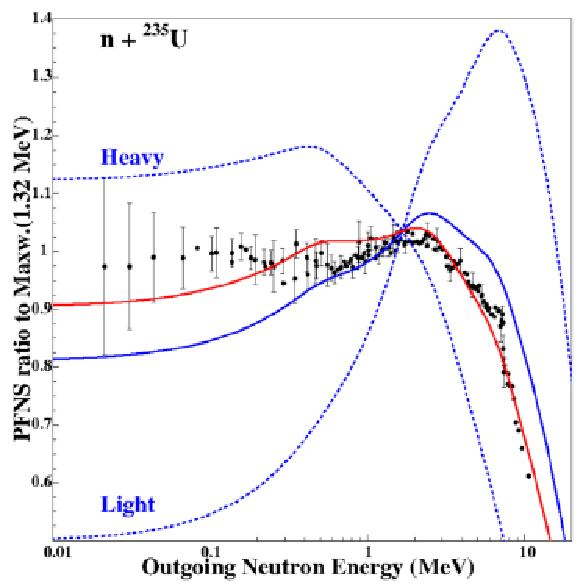
\includegraphics[width=0.90\linewidth]{images/SpecLH}
    }
    \caption{Описание спектра нейтронов как испарение асимметричных осколков деления \cite{Capote16}.}
    \label{fig:USpecLH}
  \end{figure}
  На Рис.~\ref{fig:USpecLH} показано, как пытались усовершенствовать описание спектра прямых нейтронов деления, используя независимое испарение лёгкого и тяжёлого осколков.
  Поскольку деление актинидов асимметрично, то есть один осколок чаще всего значительно меньше другого, а переданные им импульсы примерно равны, скорость лёгкого (Light) осколка значительно больше скорости тяжёлого (Heavy) осколка.
  На Рис.~\ref{fig:USpecLH}, где показано распределение по логарифму энергии нейтронов, это выражено тем, что максимум спектра нейтронов тяжёлого осколка (левая синяя штриховая кривая), соответствующий скорости тяжёлого осколка, находится при значительно меньшей энергии, чем максимум спектра лёгкого осколка (правая синяя штриховая кривая).
  Таким образом удаётся заполнить нейтронами тяжёлого осколка одиозный минимум в спектре лёгкого осколка (суммарная синяя сплошная кривая), но всё равно рассчитанные нейтроны низких энергий лежат значительно ниже экспериментальных данных.
  Ситуацию пытаются поправить эмпирически, снизив вклад лёгкого ядра до 70\% и увеличив вклад тяжёлого ядра до 130\% (красная кривая), ссылаясь на разную множественность испарительных нейтронов, но и этот вариант лежит ниже экспериментальных данных.
  
    \begin{figure}[ht]
    {
       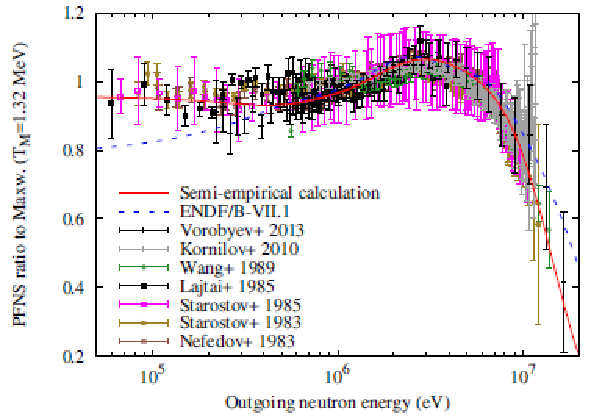
\includegraphics[width=0.90\linewidth]{images/SpecU235}
    }
    \caption{Описание спектра нейтронов деления $^{235}U$ (по \cite{Capote16}).}
    \label{fig:SpecU235}
  \end{figure}
  На Рис.~\ref{fig:SpecU235} показаны результаты измерения спектра прямых нейтронов деления $^{235}U$, сделанные в последнее время.
  Для сравнения показана аппроксимация из базы данных ENDF(VII.1) \cite{ENDF/B-VII.1} (синяя штриховая кривая), которая пока используется и в программном комплексе ТРТ для моделирования большинства нейтрон-ядерных взаимодействий.
  Она демонстрирует результат устоявшегося взгляда на генерацию прямых нейтронов при делении.
  Видно, что для мягких нейтронов аппроксимация почти на 20\% занижена, а при высоких энергиях (выше 10 МэВ) существенно завышена, причём превышение растёт с ростом энергиии нейтронов, что может приводить к существенной ошибке при моделировании реакторов на быстрых нейтронах.
  Постепенно избавляясь от теоретического взгляда, занижающего спектр нейтронов вследствие движения осколков, экспериментаторы стали замечать, что мягких нейтронов больше, чем предсказывается теоретически.
  Пионерскими работами, развеявшими миф о независимой генерации нейтронов движущимися осколками деления стали советские работы \cite{Nefed83,Starost83,Starostov85} (Nefedjv-Starostov), подтверждённые в работе \cite{Lajtai85} (Lajtai) при низких энергиях и в работе \cite{Wand89} (Wang) при высокой энергии.
  Недавние измерения \cite{Kornilov10,Vorobyev13} (Vorobyev-Kornilov) подтвердили отсутствие падения при уменьшении энергии нейтрона по сравнению с обычным распределением Максвелла для покоящейся системы.
      
    \begin{figure}[ht]
    {
       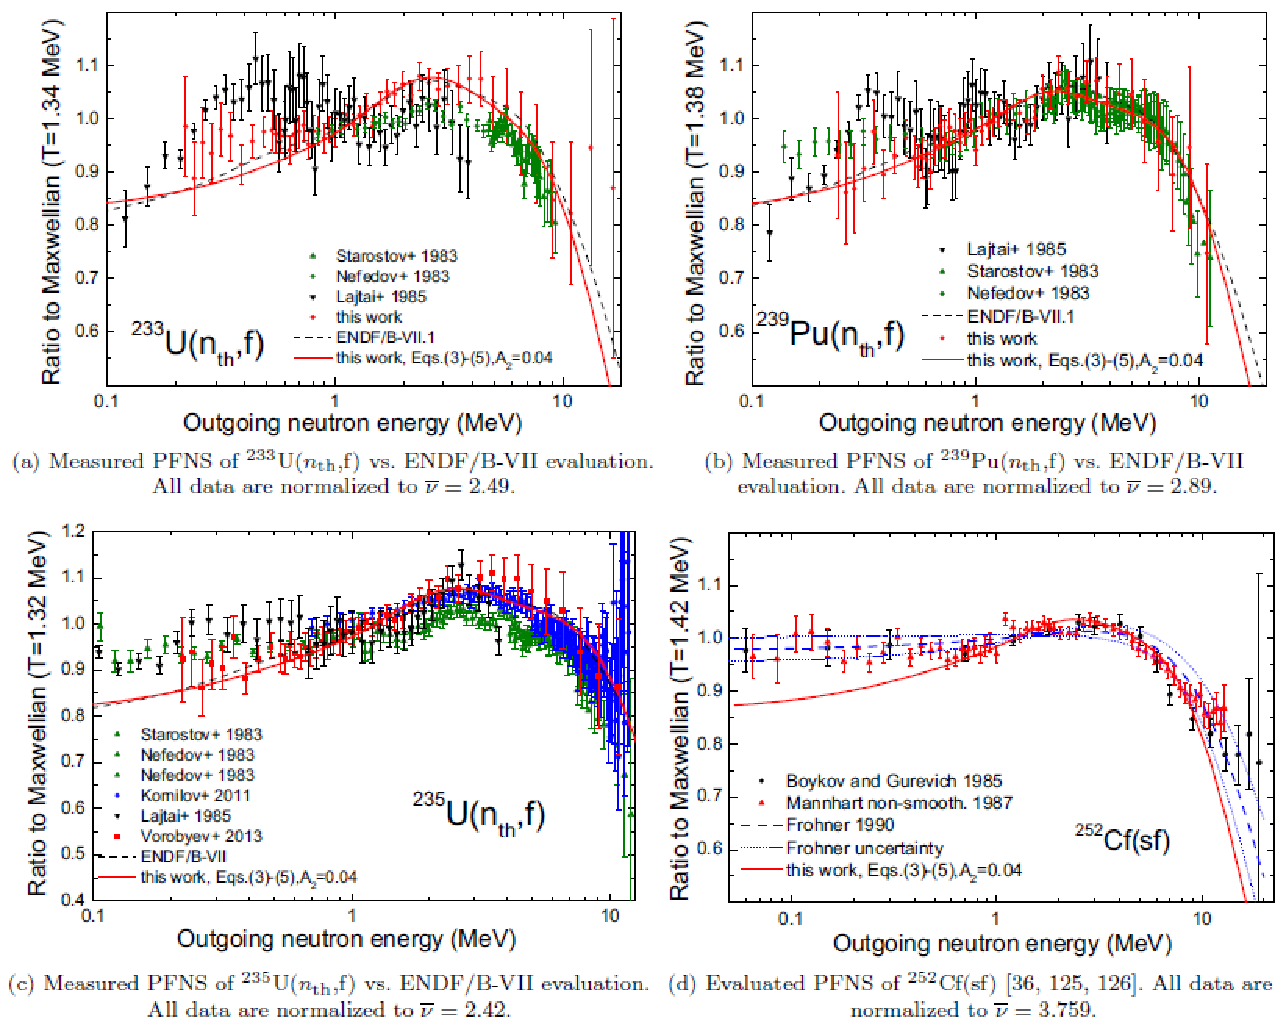
\includegraphics[width=0.90\linewidth]{images/SpecActinid}
    }
    \caption{Описание спектров нейтронов деления актинидов (по \cite{Capote16}).}
    \label{fig:SpecActinid}
  \end{figure}
  На Рис.~\ref{fig:SpecActinid} показаны относительные к максвелловскому распределению спектры прямых нейтронов деления для различных актинидов.
  Красные кривые соответствуют базе данных ENDF(VII.1) \cite{ENDF/B-VII.1}, по-прежнему настаивающей на модели испарения движущихся осколков, хотя и в более сложном виде.
  Как было показано на Рис.~\ref{fig:SpecU235} для подробно изученного ядра $^{235}U$ этот подход уже опровергнут, и при малых энергиях распределение можно считать максвелловским, как и на заре изучения деления.
  Достаточность максвелловского распределения для мягких нейтронов особенно хорошо видна на примере спонтанного деления $^{252}Cf$, однако для этого ядра база данных ENDF(VII.1) \cite{ENDF/B-VII.1} занижает спектр жёстких нейтронов.
  Если отвлечься от низких точек для мягких нейтронов, полученных в работе \cite{Lajtai85} (Lajtai), где переоценивалось вычитаемое замедление нейтронов, то можно считать, что и для $^{233}U$, и для $^{239}Pu$ в области мягких нейтронов распределение также близко к максвелловскому.
  Кроме того, можно заметить, что с увеличением атомного веса актинида температура  максвелловского распределения растёт от 1.32 до 1.42 МэВ.
  
      \begin{figure}[ht]
    {
       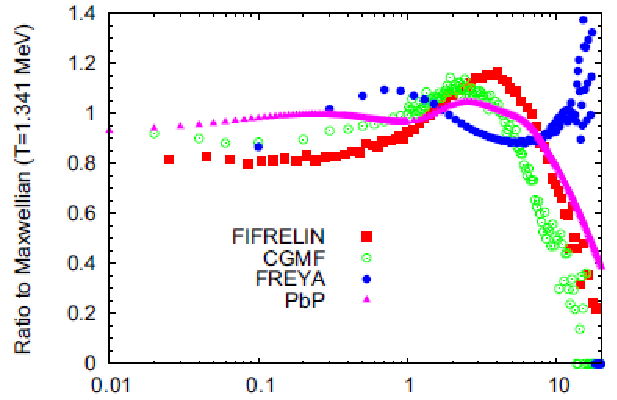
\includegraphics[width=0.90\linewidth]{images/SpecModels}
    }
    \caption{Модели, описывающие спектр прямых нейтронов деления (по \cite{Capote16}).}
    \label{fig:SpecModels}
  \end{figure}
  На Рис.~\ref{fig:SpecModels} показана эволюция моделей, описывающих спектр нейтронов деления.
  Модель FIFRELIN (красные точки) приблизительно соответствует модели испарения двух движущимися осколков деления, которая используется и в базе данных ENDF(VII.1) \cite{ENDF/B-VII.1}.
  Более поздняя модель CGMF (зелёные точки), которая развивалась в рамках проекта MCNP \cite{MCNPX} несколько уменьшила занижение спектра мягких нейтронов и при этом сделала спектр более мягким, поскольку энергия в этой модели расходуется не только на нейтроны, но и на $\gamma$-излучение.
  Противоположные по сравнению с традиционной FIFRELIN отклонения от максвелловского спектра характерны для программы FREYA (Fission Reaction Event Yield Algorithm) \cite{FREYA1,FREYA2}, которая пытается эксклюзивно описать процесс деления.
  При этом выход жёстких нейтронов в этой модели сильно завышается, поскольку для вылетающих нейтронов нет близких кинематических ограничений, зато максимум отклонения от максвелловского спектра перемещается в область ниже 1 МэВ, что не согласуется ни с одной из моделей.
  Рассмотрим, наконец, сложную матричную аппроксимацию данных PbP (Point-by-Point) \cite{PbP}, которая, фактически, является методом усреднения экспериментальных данных, не пытающимся ни сохранить энергию и импульс, ни выявить какие-то законы процесса деления.
  Это, фактически, усреднение данных, приведённых на Рис.~\ref{fig:USpecLH} и Рис.~\ref{fig:SpecU235}.
  Видно, что если этому усреднению дать 5\%-ную ошибку, то вплоть до энергии 7 МэВ отклонениями от распределения Максвелла можно пренебречь.
  Но приблизительно этой величине соответствует и энергия отделения нейтрона в актинидах. Это и является ключом к ТРТ модели, генерирующей прямые нейтроны.
  
  Развиваемая ТРТ модель исходит из того, что нейтроны начинают излучаться не тогда, когда осколки разлетелись, а тогда, когда ядро только разделилось, и кулоновское отталкивание ещё не разогнало осколки до заметной скорости.
  Именно тогда из-за большого числа степеней свободы и нейтрон-нейтронных корреляций происходит термализация нейтронов в лабораторной системе.
  Дело в том, что время жизни нейтрон-избыточного ядра меньше, чем время деления.
  Почему же учёные стали искать альтернативу простой термодинамической модели генерации прямых делительных нейтронов? -- Потому, что после 7 МэВ максвелловский спектр резко обрывался.
  В ТРТ модели этому даётся объяснение: при делении возникает фаза свободных, уже отделившихся от ядра нейтронов и фаза связанных в делящемся ядре нейтронов.
  Нейтронные перерассеяния термализуют свободную фазу, но, если в ней образуется жёсткий нейтрон с энергией больше энергии отделения нейтрона (около 7 МэВ), то такой нейтрон вступает в $(n,2n)$ реакцию с осколками деления и выбивает дополнительный нейтрон, теряя при этом энергию на отделение нового нейтрона.
  Именно эта замедляющая связанная фаза и определяет быстрое падение спектра прямых нейтронов.
  Когда ядерные фрагменты разгоняются кулоновским барьером, генерация прямых нейтронов уже прекращается.
  
\subsection{Радиационная стойкость ядерных установок.}
\label{subSol3}

	Важным применением алгоритма является моделирование радиационной стойкости материалов ядерных установок в условиях интенсивного нейтронного потока, в частности, распухания и охрупчивания различных материалов под действием нейтронов.
  
  \begin{figure}[ht]
    {
       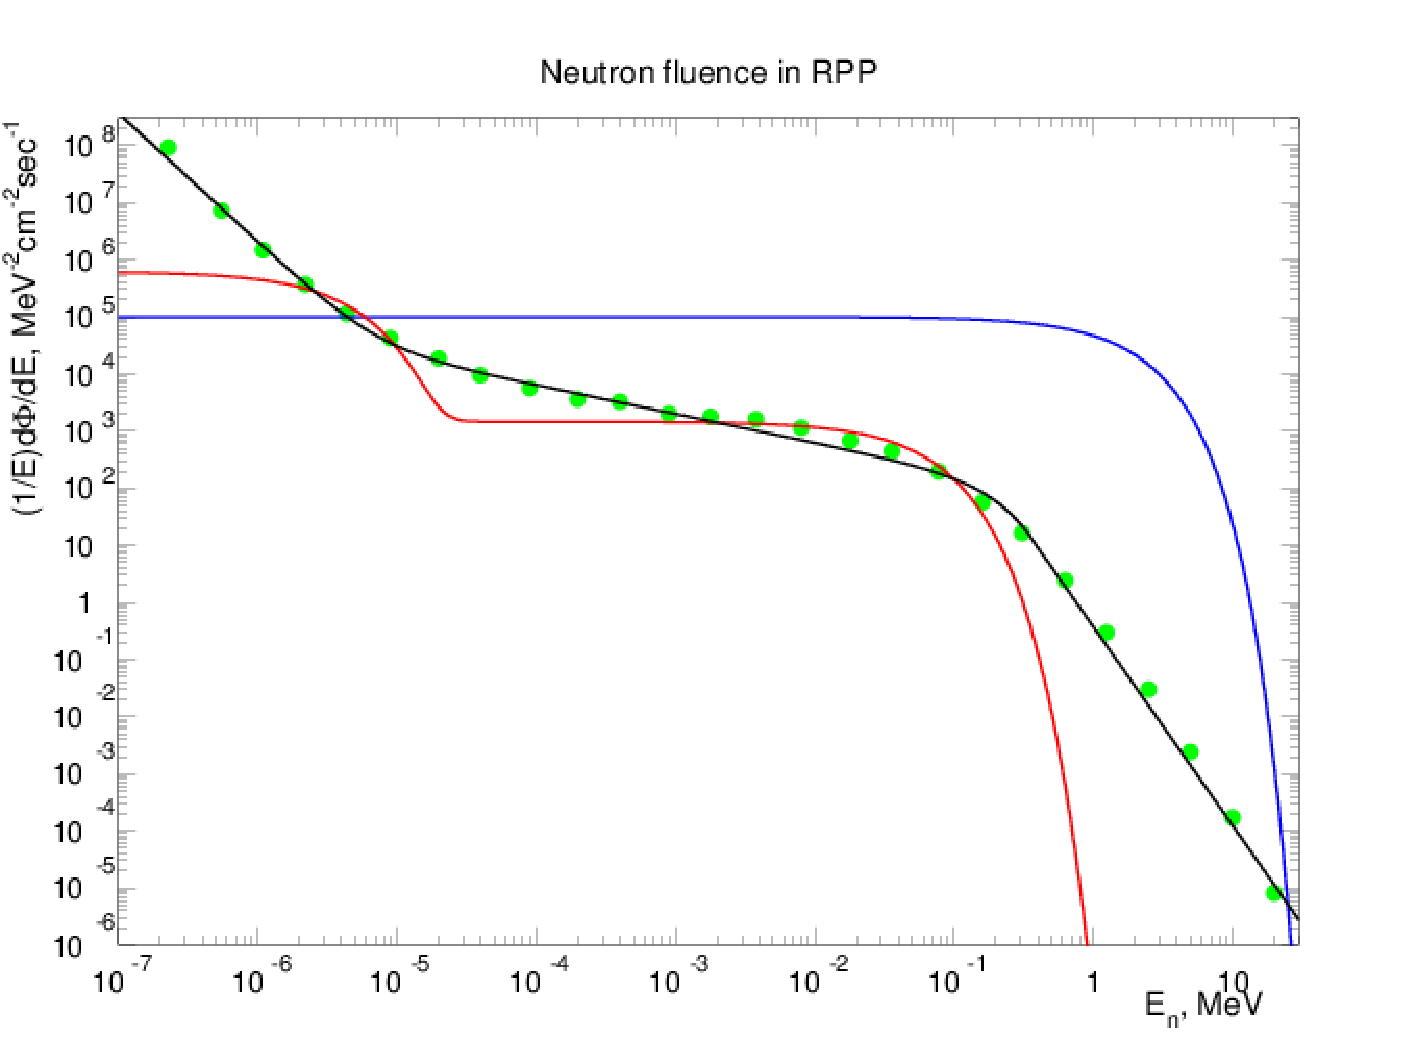
\includegraphics[width=0.90\linewidth]{images/nspec_rpp}
    }
    \caption{Флюенс нейтронов в исследовательском ядерном реакторе \cite{Aldrich83}.}
    \label{fig:SpecRPP}
  \end{figure}
  На Рис.~\ref{fig:SpecRPP} показан типичный флюенс нейтронов, делёный на энергию, за пределами корпуса реактора.
  Зелёные точки -- результат измерений, сделанных в работе \cite{Aldrich83}.
  Для сравнения синей сплошной кривой показан делённый на энергию флюенс прямых нейтронов деления, который обсуждался в предыдущем разделе.
  Видно, что нейтроны, рассеиваясь, замедляются и возникают тепловые (мягкие) нейтроны.
  Однако, вторичный флюенс невозможно свести к двум температурам -- к сумме двух экспонент, которая представлена красной кривой.
  Возникает неравновесный в смысле термодинамики флюенс (чёрная ТРТ кривая), который всё же тянется до 20 МэВ, то есть многие жёсткие нейтроны выходят из корпуса реактора, потеряв лишь малую часть своей энергии, поскольку рассеивались главным образом вперёд, но таких нейтронов очень мало.

  \begin{figure}[ht]
    {
       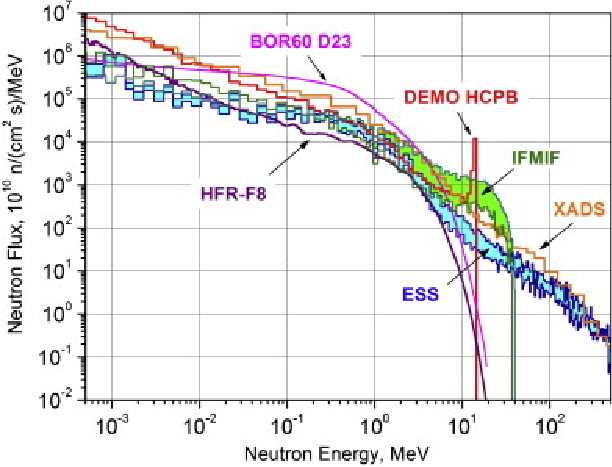
\includegraphics[width=0.90\linewidth]{images/FusionReactors}
    }
    \caption{Флюенс нейтронов в различных источниках нейтронов.}
    \label{fig:FusReac}
  \end{figure}
  На Рис.~\ref{fig:FusReac} показаны потоки нейтронов в различных источниках нейтронов.
  Флюенс (не делённый на энергию по сравнению с Рис.~\ref{fig:SpecRPP}) в обычном ядерном реакторе (показан для исследовательского реактора HFR-F8) падает уже к 20 МэВ.
  В бридере, представленном реактором BOR60 D23, флюенс нейтронов несколько жёстче (приближен к делительному спектру), но имеет практически те же пределы по энергии.
  Для того, чтобы исследовать радиационную стойкость материалов Токамака, используется нейтронный DT генератор, ускоряющий ионы водорода для увеличения вероятности $d+t\rightarrow \alpha+n$ реакции.
  Нейтрон-ядерные реакции инициируют в конструкционных материалах ядерные реакции, которые замедляют нейтроны.
  Однако этот нейтронный источник имеет энергетический предел 14 МэВ, то есть даже меньше, чем в исследовательских реакторах, зато в области 10 МэВ генерируется поток нейтронов на несколько порядков превышающий флюенс исследовательских реакторов.
  Чтобы продвинуться в область б\'{о}льших энергий нейтронов и исследовать их разрушительную силу, была создана установка IFMIF (International Fusion Materials Irradiation Facility).
  В этой установке дейтерий ускорялся до десятков МэВ и падал на тритиевую мишень, взаимодействие с которой добавляло нейтронам порядка 15 МэВ.
  Но уже в IFMIF на ускорение затрачивалось больше энергии, чем добавлялось в реакции синтеза, поэтому дальнейшее развитие пошло по пути повышения энергии ускоренной частицы (протона вместо дейтрона и тяжёлого вещества вместо трития в мишени).
  На рисунке показан спектр установки XADS (eXperimental Accelerator Driven System), в которой протоны ускорялись до энергии 600 МэВ и направлялись на жидкую, прокачиваемую для теплоотвода свинцово-висмутовую эвтектику.
  Соответственно, и спектр нейтронов тянется до полу-ГэВа.
  В США построена и в 2007 году запущена установка SNS (Spallation Neutron Source) в котором протоны с энергией 1000 МэВ облучают жидкую прокачиваемую ртуть (1 МВт, до 60 Гц).
  Соответственно на этой установке спектр нейтронов тянется почти до 1 ГэВ.
  Сейчас в UPSALA (Швеция) строится более мощный европейский аналог, в котором протоны будут ускоряться до энергии 2000 МэВ (5 МВт, 14 Гц) и будут падать на вращающееся пятитонное вольфрамовое колесо, тогда можно будет исследовать разрушительную силу нейтронов с энергиями практически достигающими 2 ГэВ.

	Нейтрон сам по себе не разрушает материал, поскольку не имеет энергетических потерь, обусловленных электромагнитными взаимодействиями с веществом.
	Нейтрон может упруго рассеяться на ядрах материала или участвовать в различных неупругих реакциях с излучением вторичных $\gamma$-квантов и заряженных ядерных фрагментов, включая радиационный захват нейтрона ядром и последующий гамма-каскад.
	Несмотря на то, что реакции с образованием вторичных ионов могут быть существенны, из-за дальнодействия электромагнитных сил, наибольшая энергия передаётся ядрам материала в результате упругого рассеяния, особенно, если материал содержит водород, отбирающий у нейтрона почти половину энергии.
	Это утверждение справедливо даже для сильных поглотителей нейтронов таких как бор, кадмий или гадолиний.
	Именно поэтому вместо того, чтобы старить материал с помощью длительного облучения нейтронами, используются интенсивные пучки эквивалентных ионов, имитирующие старение только вплоть до глубины Брэговского пика, поскольку ионы небольшой энергии не проникают на большую глубину, на которую могут проникать нейтроны.
	Если образование дефектов при нейтронном облучении более или менее однородно, то при ионном облучении плотность дислокаций может увеличиваться с глубиной проникновения и обрываться в районе пика Брэга, достигая в этой области максимума.
	Чтобы увидеть это различие, ионы ускоряют до энергий в десятки МэВ на нуклон и облучают относительно тонкие пластинки, чтобы ионы проходили насквозь, но это требует достаточно мощных ускорителей.
	Все эти нюансы повышают роль качественного сравнительного моделирования старения с помощью нейтронного и ионного облучения.
	Если даже моделирование ионного транспорта неидеально, неточности до некоторой степени сокращаются в отношении ионного и нейтронного распределений образованных Френкелевских пар.

	Заметим, что для моделирования разрушений в нейтронных полях недостаточно нейтронного и ионного транспорта.
	Для моделирования распухания и охрупчивания необходимо после остановки ионов и превращения их в нейтральные атомы применить методы молекулярной динамики, которые позволили бы описать дрейф вакансий и междоузлий с учётом эффекта их кластеризации и повышения температуры материала в результате его облучения.
	Неоднородное повышение температуры может приводить к дополнительным дислокациям, не связанным с образованием Френкелевских пар.
	При точном моделировании необходимо одновременно учитывать образование термических дислокаций и Френкелевских пар, поскольку они могут усиливать друг друга.
	Можно рассмотреть независимые диффузные модели с эмпирическим взаимодействием Френкелевских пар и дислокаций, которые позволили бы избежать расчёта взаимодействия всех атомов, рассматривая лишь диффузию и взаимодействие дислокаций, вакансий и междоузлий в непрерывной среде.
	Диффузное моделирование можно производить средствами ТРТ, определив взаимодействующие квазичастицы при диффузии в твёрдом теле.
	
	Метод оформления результатов ТРТ-моделирования ионных каскадов, инициированных жёсткими ионами или нейтронами, прост: на месте упругого рассеяния при условии, что переданная энергия оказалась больше пороговой, образуется вакансия, а на месте остановки иона или при снижении его энергии до порогового значения образуется междоузлие.
	В последнем случае указывается остаточный импульс междоузлия.
	Вакансии и междоузлия могут рекомбинировать или образовывать кластеры, а затем поры, нити и даже трещины.
	Законы диффузии атомов в кристаллических структурах в последнее время подробно исследуются.
	В частности в кремний имплантируются атомы инертных газов такие как криптон и ксенон \cite{Fried2015}.
	Энергия имплантируемых ионов составляет сотни кэВ, так что для чистоты эксперимента очень важно правильно моделировать возможные ионные каскады, которые могут вносить поправки в молекулярно-динамические расчёты, поскольку учитывают частичную ионизацию атомов, которую молекулярная динамика не принимает во внимание.

	Особняком стоит задача радиационной стойкости материалов под действием космического излучения.
	Космическое излучение также пытаются имитировать облучением ионов, однако физика процессов в корне различна.
	Ионы лишь ионизуют атомы и передают энергию ядрам вещества, а космические лучи высокой энергии рождают мезоны. Нейтральные мезоны распадаются на жёсткие гамма-кванты, инициирующие локальные электромагнитные ливни, положительные мезоны распадаются до позитронов, излучая невзаимодействующие нейтрино, а отрицательные мезоны поглощаются ядром и производят большое количество вторичных нейтронов.
	Достаточно сказать, что при аннигиляции антипротонов около 70\% энергии уносят нейтроны \cite{CHIPS_AP}, а потому, моделируя радиационную стойкость по отношению к космическим лучам, надо аккуратно моделировать радиационную стойкость по отношению к нейтронам.
	Мы уже участвовали в подобных расчётах \cite{70/435-T}, и было отмечено, что характер радиационного воздействия космического излучения существенно отличается от воздействия ионов даже с энергией в несколько десятков МэВ/нуклон, поэтому даже при одинаковых ионизационных потерях воздействие на материал будет совсем другим.
	Несмотря на это отличие, было проведено моделирование, используя ионную физику международного интерфейса Geant4, и было обнаружено, что при использовании различных имеющихся в Geant4 алгоритмов моделирования транспорта ионов имеется очень большой разброс в результатах моделирования, поэтому для надёжного моделирования радиационной стойкости материалов под действием космических лучей необходимо существенно усовершенствовать и верифицировать алгоритмы транспорта ионов и генерации адронных ливней при высокой энергии.
	Для этого существует уникальная алгоритмическая база, поскольку библиотеки физических алгоритмов CHIPS-TPT включают алгоритмы адрон-ядерного взаимодействия при высоких энергиях, апробированные на моделировании установок Большого Адронного Коллайдера.

\clearpage
\section{Энергетические потери заряженных частиц}
\label{dEdx}

  При транспорте ионов возможно не только упругое рассеяние на ядрах вещества (ядерные потери энергии), но и возбуждение вплоть до ионизации атомов материала, причём при повышении энергии ионов-снарядов возрастает вероятность не только ионизации атомов, в том числе кратной, но и выбивания энергичных электронов, называемых $\delta$-электронами.
  Генерация $\delta$-электронов отдельным процессом переводит часть потерянной жёсткой заряженной частицей энергии в энергию вторичных $\delta$-электронов, а значит эта энергия должна быть вычтена из непрерывных атомных (электронных) потерь иона, но за этим не всегда следят, считая энергию $\delta$-электронов пренебрежимо малой по сравнению с полными потерями энергии.
  При низких энергиях доля потерянной энергии, приходящейся на $\delta$-электроны, действительно пренебрежимо мала, но если будет поставлена задача расчёта потерянной энергии для жёстких ионов космических лучей, атомные потери на возбуждение и ионизацию надо будет отделять от потерь на образование энергичных $\delta$-электронов.
  Однако, это не единственное усложнение, возникающее при моделировании жёстких ионов.
  При $\gamma >> 1$ появляются и другие процессы: тормозное излучение, процесс рождения электрон-позитронных пар (процесс Бетте-Гайтлера), черенковское излучение, переходное излучение, синхротронное излучение и т. п.
  Все эти процессы пренебрежимо малы при низких энергиях, поэтому нами рассматриваться пока не будут.
  Атомные энергетические потери часто разделяются на энергетические ионизационные потери (IEL -- Ionizing Energy Loss) и энергетические потери без ионизации (NIEL -- Non-Ionizing Energy Loss).
  Принципиальная разница этих двух видов потерь заключается в том, что потери без ионизации полностью и сразу передаются материалу, нагревая его, а ионизирующие потери энергии превращаются в тепло только после электрон-ионной рекомбинации и высвечивания каскадных атомных уровней.
  Поскольку небольшая временная задержка рекомбинации для моделируемых процессов радиационной стойкости несущественна, мы не будем различать ионизационные и неионизационные потери энергии, хотя при моделировании отклика твердотельных детекторов, особенно полупроводниковых, моделировании дрейфа электронов и дырок, разделяемых электрическим полем, это может быть важно.

  Потери энергии приводят к торможению ионов.
  Рассмотрим общепринятую эмпирическую аппроксимацию электронного тормозного сечения $S_e$ для ионов низких энергий (в мэвной области).
  Ядерные потери мы будем получать прямым моделированием упругого ион-ионного рассеяния.
  Экспериментально измеренное тормозное сечение для протонов в области энергий до 10 МэВ представляется соотношением: $\frac{1}{S_e(\varepsilon)}=\frac{1}{S_{high}}+\frac{1}{S_{low}}$.
  Использование обратных величин обусловлено тем, что $S_{high}$ определяется формулой Бете-Блоха, обратная величина которого имеет максимум примерно при $\gamma=3$ ($\frac{E}{M}=2$), а при малых энергиях обратная величина $S_{low}$ описывается формулой Линдхарда в виде гиперболы $\frac{A}{v^\alpha}$, где $v$ -- скорость иона, а $\alpha$ -- порядка единицы. 
  Традиционно из-за необходимости сопряжения с формулой Бете-Блоха используют аппроксимацию: $S_{low}=A_1E^{A_2}+A_3E^{A_4}$, а для фактора, доминирующего при относительно больших энергиях, используют более сложный вид:
  \begin{equation}
  \label{Snepsilon}
  S_{high}=\frac{A_5\ln(\frac{A_6}{E}+A_7E)}{E^{A_8}},
  \end{equation}
  что является условной параметризацией формулы Бете-Блоха.
  Таким образом, описание кривой потерь является традиционно восьми-параметрическим.
  Мы описываем скейлинговую функцию семью параметрами и одним параметром сопряжения электронных и ионных потерь.
  Это сопряжение необходимо, поскольку в формулу Бете-Блоха входит максимальная кинетическая энергия, передаваемая электрону атома.
  В общем случае она записывается в виде:
  \begin{equation}
  \label{Tmax}
  T_{max}=\frac{2m_ev^2\gamma^2}{1+2\gamma\frac{m_e}{M}+(\frac{m_e}{M})^2},
  \end{equation}
  где $m_e$ -- масса электрона, а $M$ -- масса движущейся заряженной частицы (иона).
  Таким образом, для ионов $m_e << M$, и знаменатель обращается в единицу, а для электронов ($M=m_e$) в $2(1+\gamma)$.
  Именно поэтому необходим коэффициент, который сближает скейлинговую кривую для электронов со скейлинговой кривой для всех ионов, имея в виду различие в области самых низких энергий, где степень ионизации по Линдхарду зависит от заряда иона.
  Ниже мы рассмотрим это более подробно и наглядно на примере нескольких веществ.

  Подгонкой восьми коэффициентов $A_i$ можно добиться наилучшего совпадения с экспериментом для торможения протона в различных веществах. Эти коэффициенты собраны в базе данных PSTAR \cite{PSTAR}.
  Фактически эти коэффициенты используются для аппроксимации (оценки) экспериментальных данных.
  В этом смысле для выявления новых зависимостей можно использовать прямо полученные кривые энергетических потерь, что и будет нами сделано, принимая при этом во внимание то, что выбранная классическая форма аппроксимации может искажать истинную форму кривой.
  В логарифмическом масштабе PSTAR таблица тянется до 10 ГэВ, тогда как в этой области уже хорошо работает универсальная зависимость Бете-Блоха для частиц высокой энергии, которая зависит лишь от атомного состава материала.
  Тем не менее, именно в области высоких энергий вводятся поправки на эффект плотности ($\delta(\beta\gamma)$), произвольность которых сводит на нет предсказательную силу формулы Бете-Блоха при больших энергиях.
  Существенно, что, как в области до 10 МэВ, так и при б\'{о}льших энергиях в факторе эффекта плотности $\delta(\beta\gamma)$, проявляется зависимость от внутриатомной, молекулярной и кристаллической структуры, поэтому не только каждый элемент, но и каждое вещество требуют индивидуальной аппроксимации.
  Простая полуэмпирическая параметризация экспериментальных данных связана со сложностью теоретических вычислений, точность которых далека от точности имеющихся измерений, поскольку зависит от множества параметров, неизвестных для многих веществ.

  Аналогичные коэффициенты можно найти и для торможения $\alpha$-частицы в различных веществах.
  Соответствующие таблицы собраны в базе данных ASTAR \cite{ASTAR}.
  В принципе, тормозное сечение для $\alpha$-частиц можно рассчитать пользуясь масштабной инвариантностью, но, поскольку $\alpha$-частица -- это один из наиболее распространённых ионов, её тормозное сечение было с хорошей точностью измерено для многих веществ и элементов, что породило новую независимую базу данных ASTAR, доказавшую, что эмпирический скейлинг несовершенен.
  Тем не менее масштабно-инвариантный пересчёт на более тяжёлые ионы можно производить и, исходя из таблиц PSTAR для налетающего протона, и, исходя из таблиц ASTAR для альфа-частиц.
  В этом смысле точности таблицы ASTAR надо придавать не меньшее значение, чем PSTAR, причём дистанция масштабного пересчёта от ASTAR до более тяжёлых ионов короче, чем от PSTAR, поэтому в ТРТ пересчёт производится от ASTAR, а PSTAR используется только для изотопов водорода и $^3He$.
  При анализе ионизационных потерь на актинидах видно, что SRIM в максимуме занижен по сравнению с ASTAR на 5\%, а в ион-ионной физике Geant4 он занижен на 15\%.
  Более подробное обсуждение расхождений можно найти в \cite{70/241-T}.

 Тормозные сечения двух различных заряженных ионов в одном и том же веществе, обусловленные взаимодействием с электронной оболочкой атомов материала, связаны соотношением масштабной инвариантности:
  \begin{equation}
  \begin{split}
  \label{ChargeScailing}
  S_e=\frac{S_e^{ref}(f\cdot Z)^2}{(f_{ref}Z^{ref})^2} \\
  \end{split}
  \end{equation}
  где $S_e^{ref}$ и $f_{ref}$ (неэкранированная электронами часть заряда ядра) базового иона c зарядом $Z^{ref}$ вычислены для одинаковой с рассчитываемым более тяжёлым ионом ($Z$) скорости ($\beta$ или $\frac{E}{M}$).

  Полагая эффективный заряд протона полностью ионизованным ($f_p(E)\equiv$ 1), Зиглер параметризовал эффективный заряд $\gamma^\alpha(E)$ для иона гелия (ASTAR) в виде функции величины $B=\ln(\frac{E}{M})$, где $M$ - масса иона (в данном случае $\alpha$-частицы), а $E$ -- его энергия
  \begin{equation}
%  \begin{split}
  \label{Hegamma}
  f^2=1-C^2e^{-0.2865-0.1266\cdot B+0.001429\cdot B^2-0.02402\cdot B^3+0.01135\cdot B^4-0.00147\cdot B^5},
%  &\\
% \end{split}
  \end{equation}
где $C=1+(0.007+0.00005\cdot Z)\cdot e^{-(7.6-B)^2}$.
  На самом деле это выражение для величины квадрата отношения эффективной доли заряда $\alpha$-частицы к эффективной доле заряда протона
  \begin{equation}
  \label{pseudo-gamma}
    f=\frac{f_\alpha}{f_p}.
  \end{equation}
 Это поможет нам вычислить эффективный заряд протона, который обычно не приводится, но может быть интересен, в частности, для молекулярно динамических расчётов транспорта ионов водорода.
  Величина $S_e^{ref}$ протона должна быть взята при энергии $E_p=\frac{E_\alpha\cdot M_p}{M_\alpha}$, поскольку скорости протона и $\alpha$-частицы должны быть равны.

\subsection{Аппроксимация $\frac{dE}{dx}$ из PSTAR, ASTAR и ESTAR }
\label{dEdx1}
  
  Обратимся теперь к анализу кривых энергетических потерь, взятых из баз данных PSTAR, ASTAR и ESTAR, для различных веществ, состоящих из одного элемента.
  Начнём рассмотрение с аморфного углерода, при этом надо отметить, что потери энергии в графите и алмазе будут несколько отличаться, как при самых низких, так и при самых высоких энергиях.
  \begin{figure}[ht]
    {
       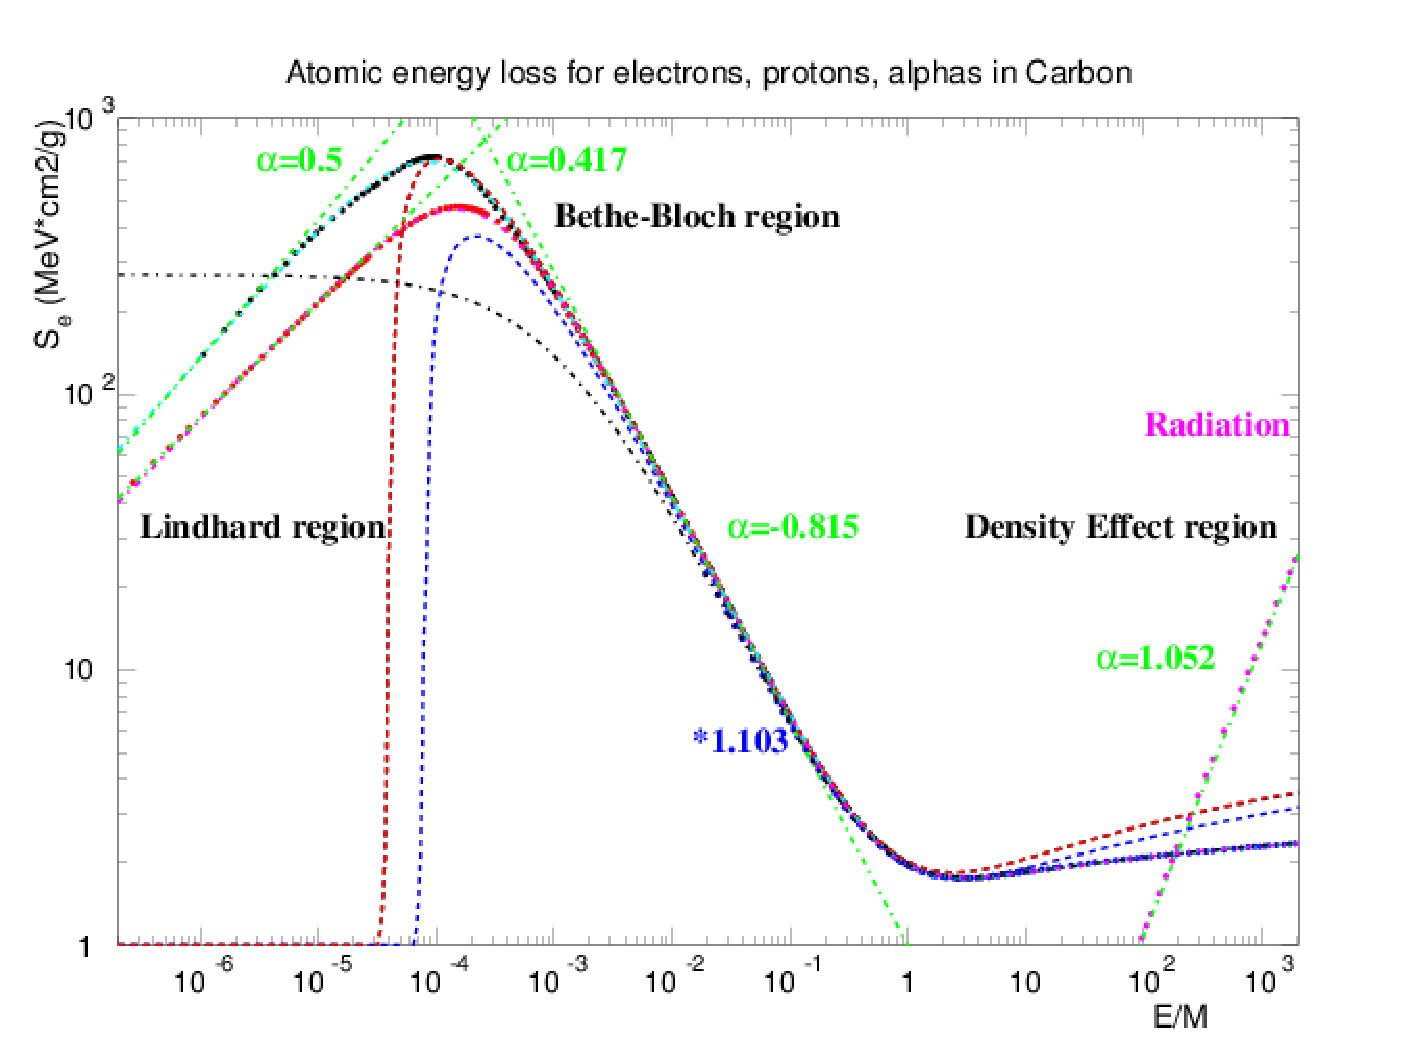
\includegraphics[width=0.99\linewidth]{images/epa_c_l}
    }
    \caption{Энергетические потери в аморфном углероде для протонов, $\alpha$-частиц и электронов в зависимости от скейлинговой переменной $y=\frac{E}{M}=\gamma-1$.}
    \label{fig:dEdxCL}
  \end{figure}
  Из Рис.~\ref{fig:dEdxCL} видно, что в области средних энергий кривые энергетических потерь для протонов (чёрные точки), $\alpha$-частиц (красные точки, поделенные на квадрат заряда $\alpha$-частицы, то есть на 4) и электронов (синие точки умножены на зарядовый коэффициент 1.103 так чтобы кривые Бете-Блоха в точности совпали при $\frac{E}{M}=0.5$) близки друг к другу.
  Пунктирами показаны соответствующие кривые формулы Бете-Блоха для этих частиц:
  \begin{equation}
  \label{BetheBloch}
    \frac{dE}{dx}=\frac{Kz^2Z}{A\beta^2}\left[\frac{1}{2}ln\left(\frac{2m_ev^2\gamma^2T_max}{I^2}\right)-\beta^2-\frac{\delta(\beta\gamma)}{2}\right],
  \end{equation}
  где $K=0.307075\frac{MeVcm^2}{g}$, $z$ -- заряд иона, $Z$ -- заряд ядер вещества, $A$ -- атомный вес вещества, $I$ -- средний потенциал ионизации, который обычно является подгоночным параметром при аппроксимации экспериментальных данных, $v=c\beta$, как и в формуле (\ref{Tmax}) для максимальной переданной энергии $T_{max}$.
  Чёрная и красная пунктирные кривые очевидно совпадают, поскольку $T_{max}$ для всех ионов одинаков, и отличие только в квадрате заряда $z^2$, на который сделана поправка.
  Видно, что электронная синяя пунктирная кривая, поправленная на постоянный коэффициент 1.103, также при средних энергиях близка к кривой Бете-Блоха для ионов, но при малых и при высоких энергиях идёт на 10-15\% ниже.
  Обрыв кривой Бете-Блоха при $\frac{E}{M}=10^{-4}$ указывает на то, что при столь малых энергиях формула теряет свою силу, и надо использовать подход Линдхарда.
  Отличие при $\gamma >> 1$ обусловлено отличием поправки на эффект плотности, который снижает величину энергетических потерь по-разному для ионов и для электронов.
  Для ионов в области высоких энергий наблюдается точное совпадение скейлинговых кривых, то есть отличие полностью описывается фактором заряда иона $z^2$.
  Отличие красной и чёрной кривых в области малых энергий связано с тем, что при уменьшении скорости иона, он начинает подхватывать электроны вещества, и его эффективный заряд снижается.

  Попробуем аппроксимировать формулу Бете-Блоха при средних энергиях, где она совпадает с реальными энергетическими потерями, то есть в диапазоне от $10^{-3}$ до $10^{-1}$.
  Поскольку кривая приведена в дважды-логарифмическом масштабе, степенная зависимость будет описываться гиперболой $\frac{1}{(1+\gamma)^\alpha}$.
  Аппроксимирующая зелёная кривая, проходящая через этот участок зависимости, соответствует степени $\alpha=0.815$.
  Эту зависимость можно экстраполировать и в область малых энергий, предположив, что эффективный заряд иона $f$ пропорционален некоторой степени скорости $v=\sqrt{\frac{2E}{M}}$, и в пределе нулевой скорости обращается в ноль, то есть ион становится нейтральным атомом.
  Для протонов Линдхард показал, что ионизационные потери растут пропорционально скорости, то есть корню из $\gamma-1$ -- зелёная прямая с показателем $\alpha=0.5$.
  Видно, что для протонов закон Линдхарда действительно выполняется, а вот для $\alpha$-частиц наклон другой -- $\alpha=0.417$, однако, как будет видно, для других материалов степень может быть не только меньше, но и больше $0.5$.
  Отметим ещё радиационный вклад, показанный в правой части рисунка и растущий практически пропорционально $\gamma$.
  Этот вклад, который становится существенен при $\gamma > 100$, аппроксимируется степенью $\alpha=1.052$.
  Превышение над единицей связано с тем, что тормозное излучение растёт пропорционально энергии, а конверсия в электрон-позитронные пары растёт несколько быстрее.
  В любом случае мы пока не рассматриваем ионы столь высоких энергий.
  При низких энергиях мы выбрали аппроксимацию $\Phi_1(y)=\frac{C_1}{y^{\alpha_1}+G\cdot y^{-\alpha_2}}$, где $y=\frac{E}{M}$, тогда при больших $x$ степенное падение определяется параметром $\alpha_1\approx 0.815$, а при малых $x$ степенной рост определяется показателем $\alpha_2=0.5$ для протонов и $\alpha_2=0.417$ для $\alpha$-частиц.
  Чтобы описать жёсткую часть кривой, была использована двух-параметрическая формула $\Phi_2(y)=C_2 [F_n(y)]^{\alpha_3}$, где функции $F_i$ определяются рекурсивным циклом: $F_0(y)=ln(1+y)$, где $1+y=\gamma$, $F_{n+1}(y)=ln(1+F_n(y))$.
  Все функции $F_i(y)$ положительно определены при всех положительных $y$.
  Чем больше $n$, тем более пологим становится рост функции энергетических потерь с ростом энергии ($y$).
  Темп роста учитывает вклад коэффициента эффекта плотности, поведение которого мы рассмотрим отдельно.
  Фактически эта часть аппроксимации зависит только от данных ESTAR.
  Финальная ТРТ аппроксимация является суммой этих двух вкладов: $\frac{dE}{dx}_{TPT}=\Phi_1(x)+\Phi_2(x)$, то есть
  \begin{equation}
  \label{TPTfitform}
    \frac{dE}{dx}=\frac{C_1}{y^{\alpha_1}+G\cdot y^{-\alpha_2}}+C_2 [F_n(y)]^{\alpha_3}.
  \end{equation}
  Соответствующая розовая кривая идёт через красные точки для $\alpha$-частиц и голубая кривая -- для протонов.
  Оцененные данные описываются нашей кривой с процентной точностью, то есть практически неотличимы от данных на рисунке, и именно эти кривые мы используем для моделирования.
  С ещё большей точностью описываются электронные потери (чёрная штрих-пунктирная кривая), но они будет обсуждаться при рассмотрении более тяжёлых материалов, для которых отличие электронной кривой при малых $y$ от ионной кривой значительно больше.
  
  \begin{figure}[ht]
    {
       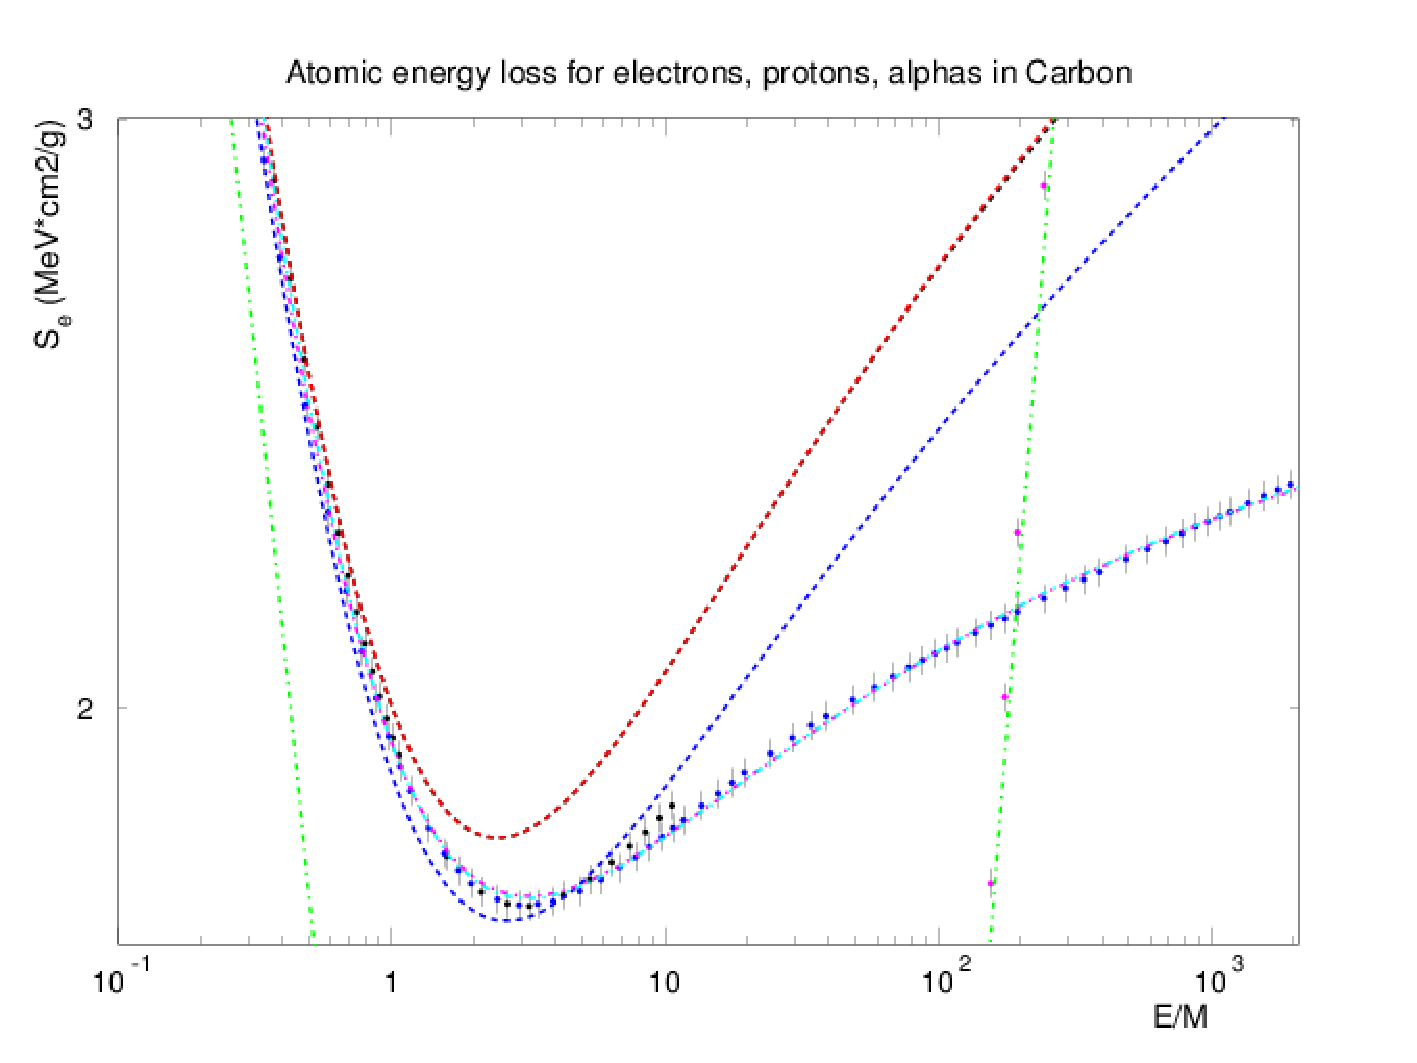
\includegraphics[width=0.99\linewidth]{images/epa_c_s}
    }
    \caption{Энергетические потери в аморфном углероде для протонов, $\alpha$-частиц и электронов в области минимальной ионизации.}
    \label{fig:dEdxCS}
  \end{figure}
  Для того, чтобы проиллюстрировать, как был подогнан параметр $\xi=1.103$, приподнимающий скейлинговую функцию потерь для электронов вследствие отрицательного заряда, покажем область минимума ионизации в увеличенном размере. 
  Из Рис.~\ref{fig:dEdxCS}, построенного в области $\frac{E}{M}$ от 0.1 до 2000, видно, что коэффициент $\xi=1.103$ совмещает протонные (чёрные) и электронные (синие) точки в области $y$ от 1 до 5, где достигается минимум ионизации.
  При б\'{о}льших $y$ протонные точки идут приблизительно на 1\% выше электронных (1\% -- это размер ошибок), но это уже соответствует энергии протонов в несколько ГэВ, а при $y < 1$ электронные точки идут несколько ниже, но мы их не используем для уточнения аппроксимации ионизационных потерь ионов.
  Можно также отметить, насколько резко возрастают потери ионов с $\gamma > 100$ из-за тормозного излучения и рождения электрон-позитронных пар (розовые точки, зелёная штриховая кривая).
  Это предел энергии ионов, для которых мы можем моделировать энергетические потери.
  При больших энергиях надо добавлять все перечисленные жёсткие процессы.
  
  Та же методика была применена для кремния.
    \begin{figure}[ht]
    {
       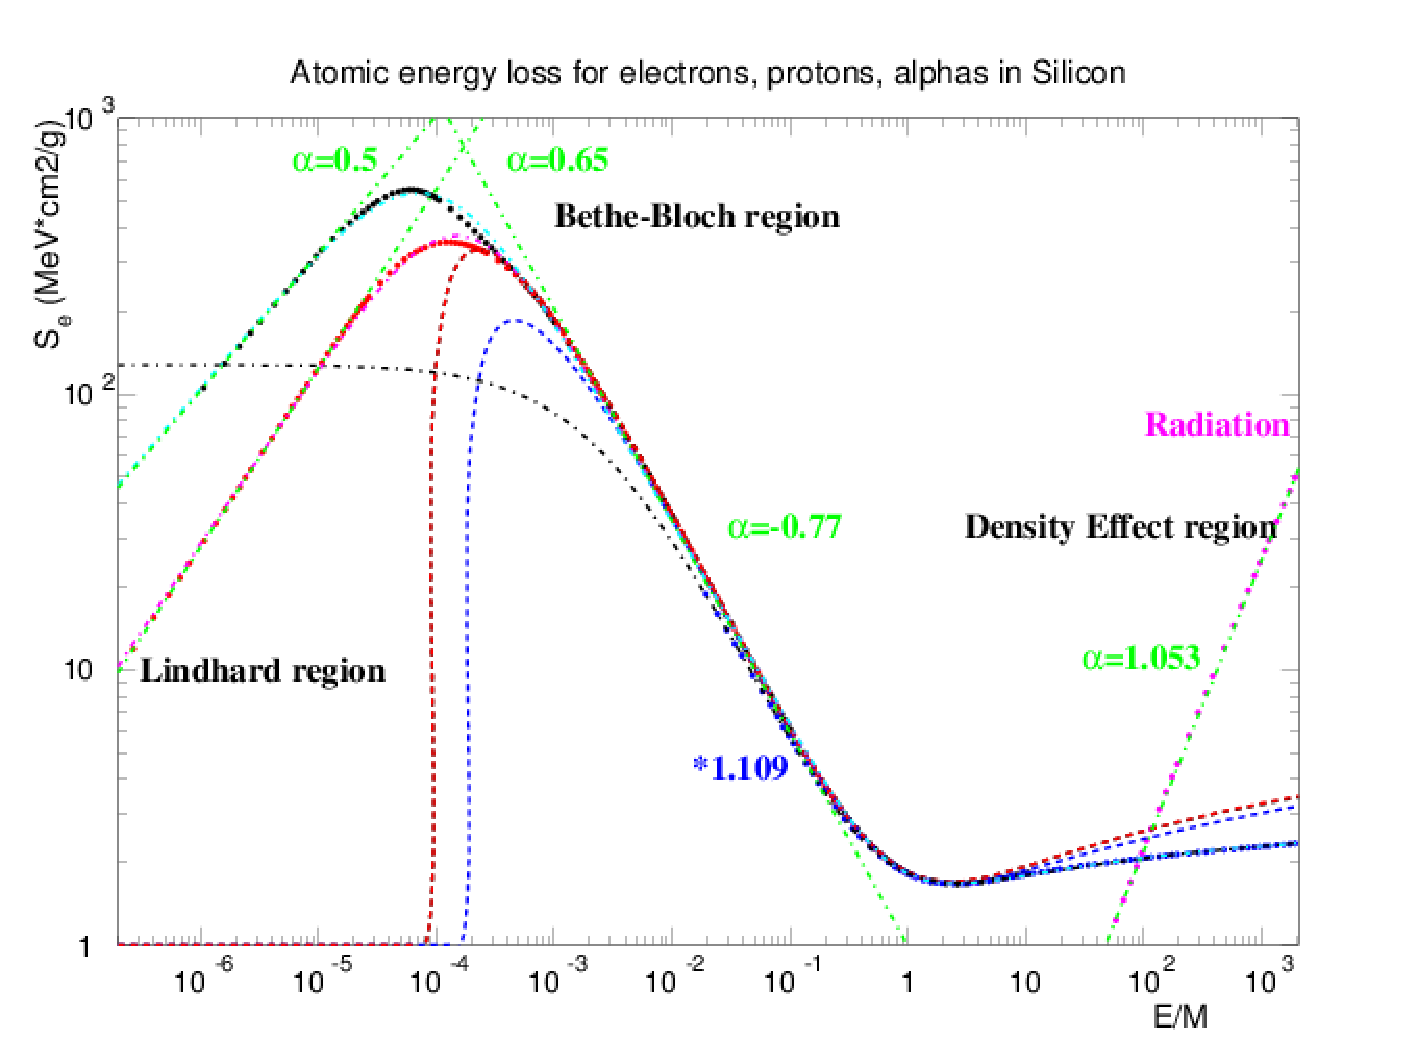
\includegraphics[width=0.99\linewidth]{images/epa_si_l}
    }
    \caption{Энергетические потери в кремнии для протонов, $\alpha$-частиц и электронов в зависимости от скейлинговой переменной $y=\frac{E}{M}=\gamma-1$.}
    \label{fig:dEdxSiL}
  \end{figure}
  На Рис.~\ref{fig:dEdxSiL} показаны аналогичные углероду кривые, аппроксимирующие скейлинговые кривые энергетических потерь для кремния.
  Обращает на себя внимание, что аппроксимация энергетических потерь $\alpha$-частиц в области малых энергий описывается степенью $\alpha=0.65$, то есть с наклоном большим, чем для протонов ($0.5$), хотя для углерода эта степень была меньше $0.5$, то есть в разных веществах степень ионизации различных ионов оказывается различной, но близкой к $0.5$.
  Это позволяет предположить, что в действительности величина $\alpha$ для $\alpha$-частиц может быть равной $0.5$ и только систематические ошибки измерений, затруднённых для малых энергий ионов, меняют степень зависимости.
  Варьируя эту величину, можно оценить её влияние на результаты описываемых экспериментов.
  Например при переходе к более тяжёлым ионам можно сравнить эту степень зависимости с имеющимися экспериментальными данными.
  Формула Зиглера (\ref{Hegamma}) пытается уловить влияние процесса ионизации на величину $\alpha$, но, сравнивая с реальным отношением из ASTAR и PSTAR, можно обнаружить отклонения до 65\% при энергиях порядка 20 кэВ, а при более низких энергиях и больше.
  Необходимы физические модели, которые бы описали различие в степенной зависимости от энергии при малых энергиях.
  Важно, что, как будет показано, практически для всех веществ зависимость энергетических потерь в области самых малых энергий -- степенная.
  Степенная зависимость обладает важнейшим свойством -- она обращается в ноль при нуле энергии.
  Отметим также, что, несмотря на то, что в области энергий, где применима формула Бете-Блоха, наклоны кривых для протонов и $\alpha$-частиц совпадают, из-за различного загиба вниз в области Линдхарда значения степеней $\alpha_1$ в фитирующей формуле (\ref{TPTfitform}) немного отличаются ($p$/$\alpha$): на углероде это 0.790/0.815, на кремнии 0.737/0.749, на германии 0.703/0.743, на гадолинии 0.676/0.716, на уране 0.653/0.672.
  Из-за более раннего загиба степень падения $\alpha$-частиц всегда немного больше, чем для протонов.
  Интересно отметить ``скейлинг'' по нормировке гиперболы в области Бете-Блоха: продолжение гиперболы почти всегда проходит через точку (1,1), то есть в формуле (\ref{TPTfitform}) $C_1\approx 1$, хотя показатель степени гиперболы $\alpha_1$, приведенный выше, меняется несколько больше, хотя они тоже не сильно отличаются.
  Значения $C_1\approx 1$: на углероде это 1.10/1.01, на кремнии 1.16/1.12, на германии 0.99/.87, на гадолинии 0.88/0.78, на уране 0.81/0.76.
  Если поделить нормировку на тривиальный множитель $Z/A$ в формуле (\ref{BetheBloch}), то получим 2.20/2.02, 2.32/2.24, 2.24/1.97, 2.16/2.46, 2.10/1.97, то есть практически константа, что и объясняет обнаруженный ``скейлинг'' для различных материалов.
  С точностью до деталей порядка нескольких процентов этот ``скейлинг'' сохраняется и для композитных материалов из разных элементов, если для них использовать усреднённую величину $\langle\frac{Z}{A}\rangle$.
  Экстраполяция кривой энергетических потерь электронов не имеет выраженного максимума.
  Особенность остановки мягких электронов будет обсуждаться при рассмотрении энергетических потерь в германии.
  Посмотрим, как изменилась $\Phi_2$, которая определяется нормировочным множителем $C_2$, рангом функции $F_n$ и степенью $\alpha_3$, в которую эта функция возводится.
  Все эти параметры коррелируют ($C_2$,$p$,$n$): для углерода (3.28,1.29,3)/(2.05,0.9,2), для кремния (35.8,2.76,6)/(14.5,2.29,5).
  То есть часть функции для высоких энергий весьма индивидуальна.
  Это связано с весьма индивидуальным поведением коэффициента эффекта плотности, который меняется даже для твёрдого/жидкого и газообразного состояния.
  Параметризацию коэффициента эффекта плотности мы рассмотрим в отдельном разделе.
  
  \begin{figure}[ht]
    {
       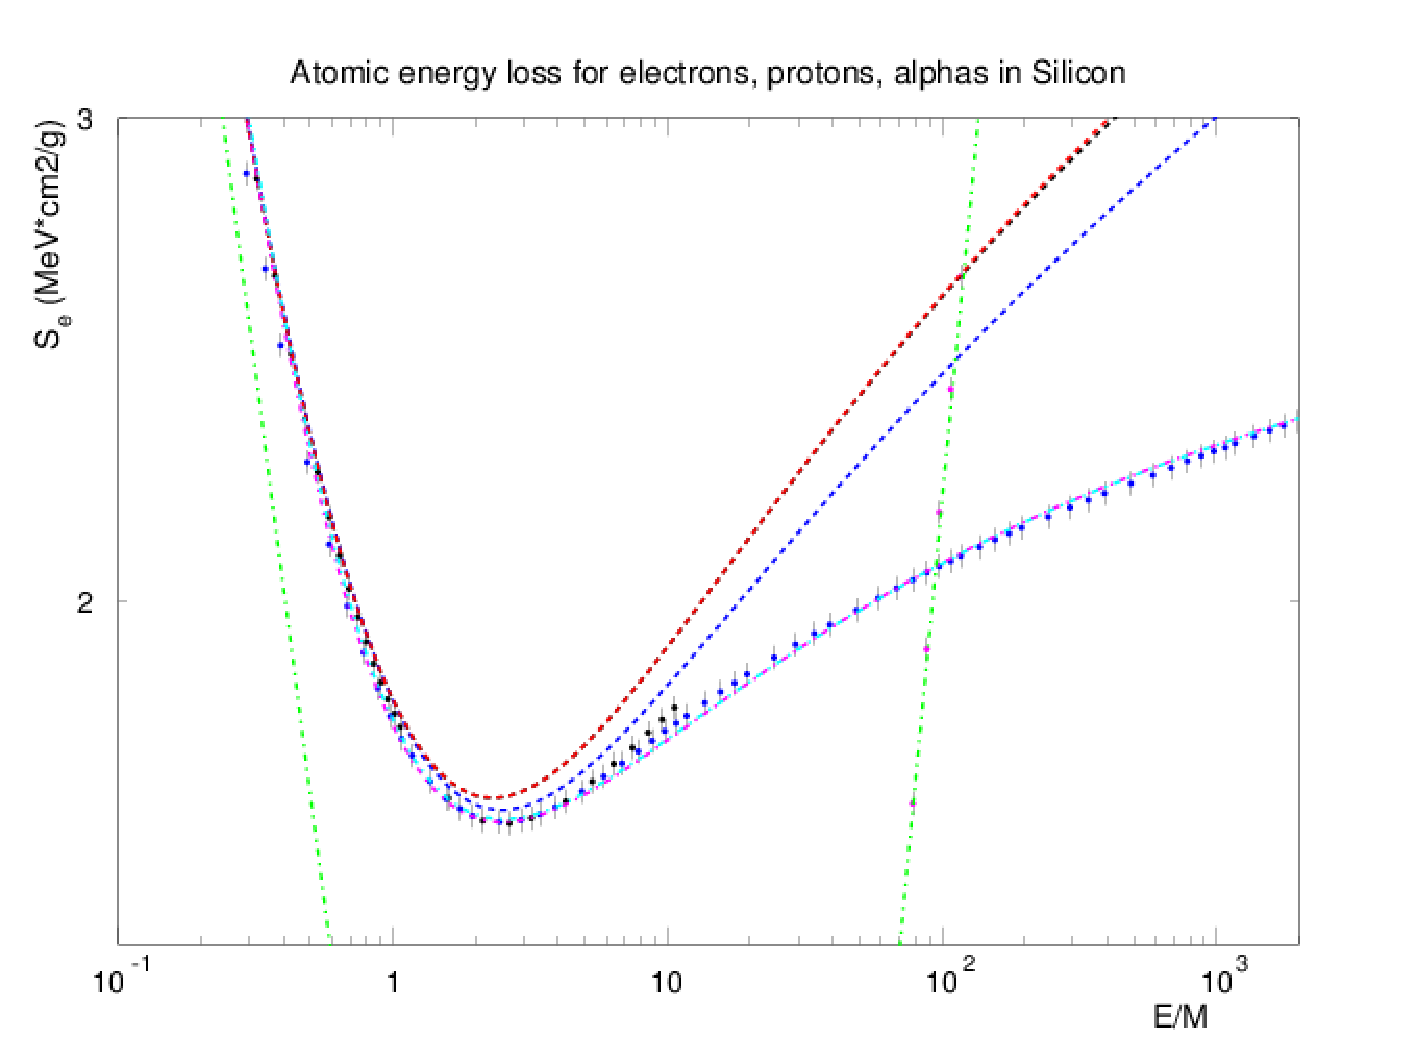
\includegraphics[width=0.99\linewidth]{images/epa_si_s}
    }
    \caption{Энергетические потери в кремнии для протонов, $\alpha$-частиц и электронов в области минимальной ионизации.}
    \label{fig:dEdxSiS}
  \end{figure}
  Из Рис.~\ref{fig:dEdxSiS}, построенного в области $\frac{E}{M}$ от 0.1 до 2000 для кремния, видно, что электронные и протонные кривые совмещены в области минимальной ионизации уже несколько большим коэффициентом: 1.109 вместо 1.103 для графита.
  Качественно этот рисунок мало отличается от Рис.~\ref{fig:dEdxCS} для углерода, доказывая лишь, что коэффициент был подобран правильно.
  Аналогичные рисунки будут приводиться и для более тяжёлых материалов.
  Тем не менее, можно отметить, что для углерода ТРТ аппроксимации (голубая и розовая кривые) в пределах 1\% идут выше данных PSTAR, а при $y=20\div 40$ в тех же пределах ниже данных ESTAR.
  Это вполне приемлемая точность для аппроксимирующей формулы с меньшим числом параметров, и только практика может определить, какая из формул лучше.
  Для кремния ТРТ кривые в точности описывают данные в минимуме ионизации, но немного занижены вблизи $y=10$ и завышены в области $y=20\div 80$.
  Это является следствием того, что для углерода использовались $F_n$-функции с $n_p=3$ и $n_\alpha=2$, а для кремния $n_p=6$ и $n_\alpha=5$.
  Параметры были найдены методом наименьших квадратов, поэтому такой выбор можно объяснить только упомянутым существенным различием в коэффициенте эффекта плотности.
  Напомним, однако, что PSTAR таблица обрывается на $y=10$, а ТРТ аппроксимация экстраполируется до сколь угодно высоких энергий, хотя в области $y>100$ нужно вводить дополнительные радиационные процессы. 
  
    \begin{figure}[ht]
    {
       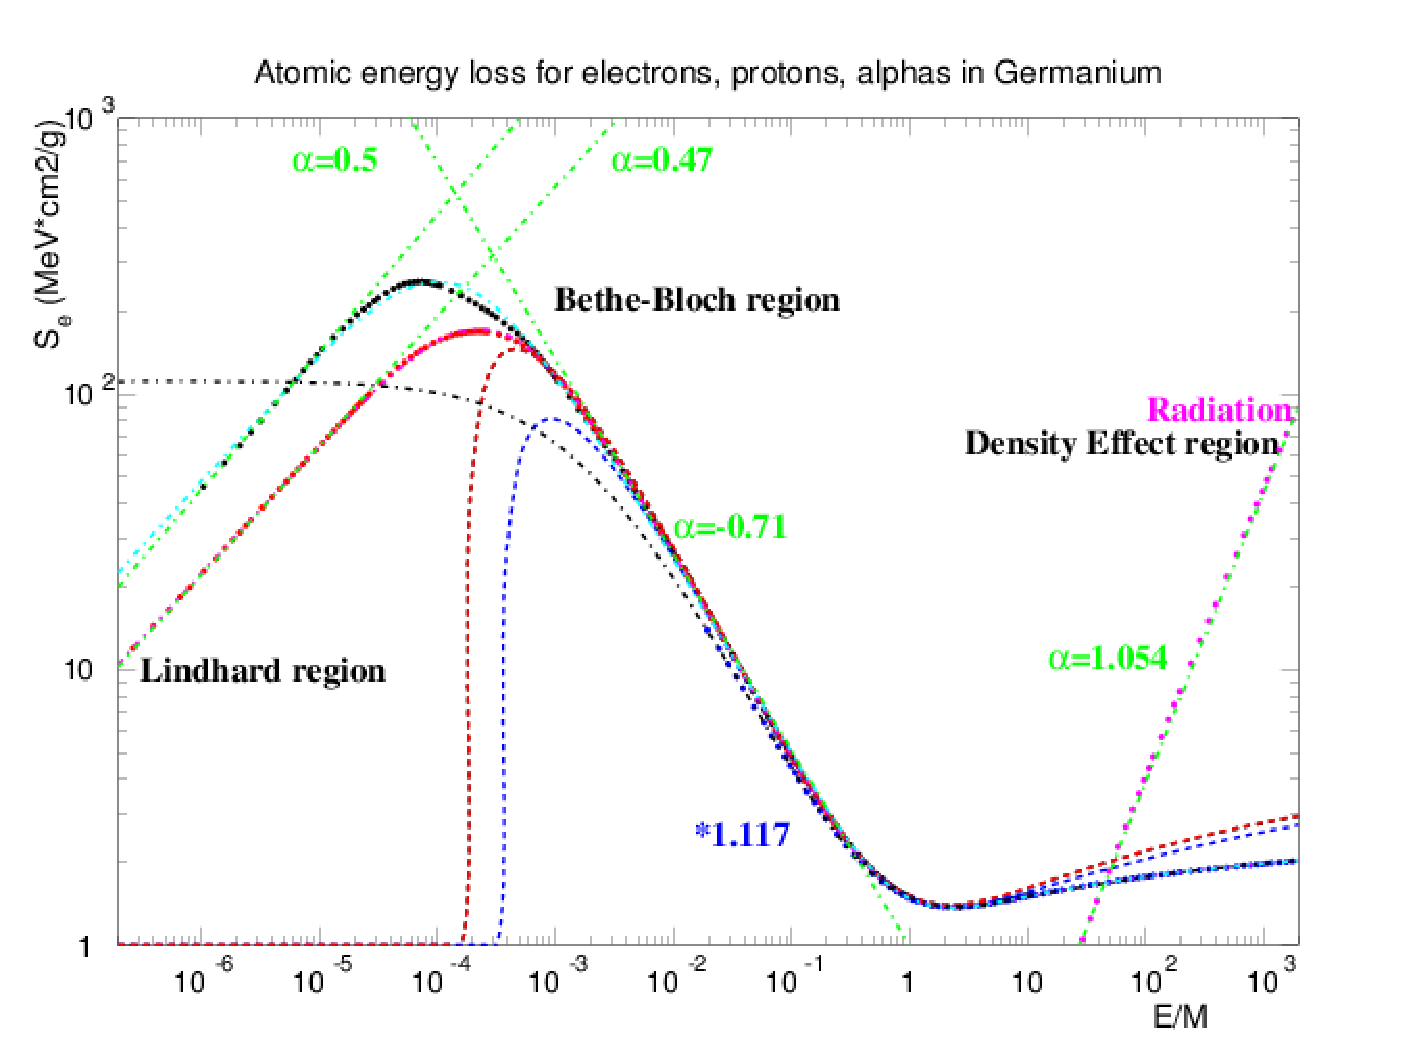
\includegraphics[width=0.99\linewidth]{images/epa_ge_l}
    }
    \caption{Энергетические потери в германии для протонов, $\alpha$-частиц и электронов в зависимости от скейлинговой переменной $y=\frac{E}{M}=\gamma-1$.}
    \label{fig:dEdxGeL}
  \end{figure}
  Для германия на Рис.~\ref{fig:dEdxGeL} показаны аналогичные кривые, аппроксимирующие потери энергии.
  Нормировочный коэффициент для электронной кривой вырос до 1.117.
  Рост этого коэффициента в зависимости от $\frac{Z}{A}$ также надо будет аппроксимировать для пересчёта электронных кривых в ионные и наоборот.
  На германии наклоны кривых для протонов и $\alpha$-частиц неожиданно сравниваются, причём зелёные оценочные кривые различны, а ТРТ аппроксимация даёт $\alpha_2=0.47$ и для протонов, и для $\alpha$-частиц.
  Единственное различие -- в том, с какой энергии начинается загиб, что определяется параметром $G$ в формуле (\ref{TPTfitform}).
  Для протонов $G_p=0.0000305$, а для $\alpha$-частиц $G_\alpha=0.000062$, то есть вдвое больше.
  Для сравнения на углероде $G_p=0.0000112$ и $G_\alpha=0.0000298$, то есть отношение больше, чем двойка, а на кремнии $G_p=0.0000105$ и $G_\alpha=0.0000059$, то есть меньше, чем 0.5.
  Это связано с тем, что на кремнии наклон для $\alpha$-частиц ($\alpha_2$) больше, чем для протонов.
  Заметим также, что и уровни минимальной, и уровни максимальной ионизации снижаются при увеличении атомного веса материала. 

  \begin{figure}[ht]
    {
       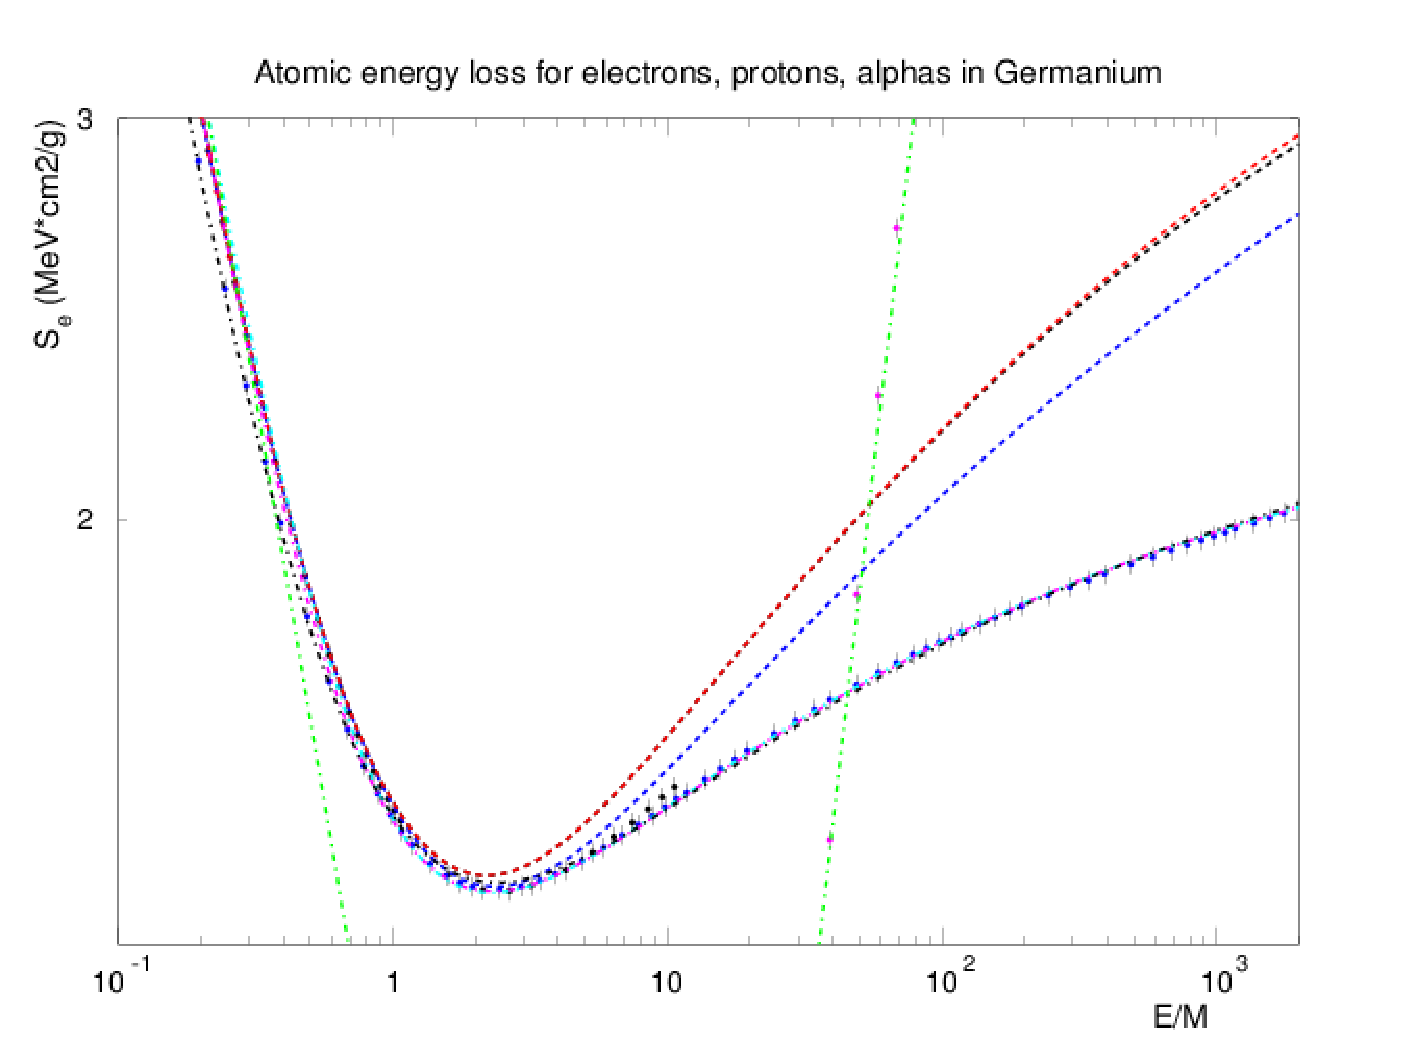
\includegraphics[width=0.99\linewidth]{images/epa_ge_s}
    }
    \caption{Энергетические потери в германии для протонов, $\alpha$-частиц и электронов в области минимальной ионизации.}
    \label{fig:dEdxGeS}
  \end{figure}
  Из Рис.~\ref{fig:dEdxGeS}, построенного в области $y=\frac{E}{M}$ от 0.1 до 2000 для германия, видно, что с увеличением атомного веса материала при совпадении в области минимальной ионизации кривые PSTAR и ESTAR сближаются и при больших $y$.
  Кроме того, можно отметить почти идеальное совпадение ТРТ кривых (голубая и розовая) в области больших $y$, чего не удавалось достичь на более лёгких материалах.
  Из рисунка видно, что с увеличением атомного веса материала при малых $y$ ESTAR кривая всё больше отклоняется от совпадающих PSTAR и ASTAR кривых, а в минимуме ионизации электронная кривая практически совпадает с кривой Бете-Блоха, то есть коэффициент эффекта плотности становится пренебрежимо мал (напомним, что кривая Бете-Блоха для электронов умножается на тот же коэффициент, что и вся электронная кривая).
  Эффект снижения энергетических потерь электронов по сравнению с соответствующими энергетическими потерями ионов связан с тем, что электроны фактически не имеют пика Брэга, поскольку их ионизационные потери при малых энергиях не имеют столь ярко выраженного максимума на кривой ионизационных потерь, какой имеют ионы.
  В результате вместо пика Брэга возникает широкий электронный каскад, своего рода электронное облако с диаметром, исчисляемым ангстремами.
  Такое электронное облако очень опасно с медицинской точки зрения, поскольку способно произвести двойной невосстановимый разрыв в спирали ДНК.
  В материаловедении такое облако может создавать дислокацию в кристаллической структуре, поэтому электроны тоже надо транспортировать до точки рекомбинации.
  К сожалению, ESTAR таблицы дают энергетические потери электронов только выше 10 кэВ, то есть при энергиях, характерных только для $\delta$-электронов, но не для электронов ионизации, возникающих в огромном количестве вдоль трека заряженной частицы.
  Очень важно экстраполировать энергетические потери электронов в область самых малых энергий.
  Такая ТРТ-аппроксимация показана на рисунке чёрной штрих-пунктирной кривой.
  Метод наименьших квадратов требует очень малой величины наклона $\alpha_2$, поэтому её пришлось ограничить минимальной величиной 0.001, то есть энергетические потери становятся практически независящими от энергии.
  Протоны останавливаются по закону: $\frac{dE}{dx}\propto -v$, или для скорости $\frac{dv}{dx}=-B$, то есть скорость пропорциональна расстоянию до точки остановки.
  Электроны останавливаются по закону: $\frac{dE}{dx}=-const$, то есть энергия пропорциональна расстоянию до точки остановки.
  Перепишем это через скорость: $\frac{vdv}{dx}=-const$, заменяя $dx$ на $v\cdot dt$, получаем: $\frac{dv}{dt}=-const$, то есть движение останавливающихся электронов является равнозамедленным, то есть его можно описать эффективной силой трения для электрона в среде.
  Таким образом, каскад электронной остановки моделируется очень легко: электрон движется равнозамедленно под действием силы трения, и, когда энергия торможения вдвое превосходит среднюю энергию ионизации, электрон продвигается на расстояние, соответствующее половине его энергии.
  Вторая половина энергии, соответствующая работе силы трения, за вычетом половины энергии ионизации (половина энергии ионизации вычитается и из энергии лидирующего электрона) передаётся другому электрону, и так развивается каскад, пока энергия электрона не станет меньше двух средних энергий ионизации.
  Такой мягкий электрон просто выделяет энергию на последнем шаге и образует отрицательный экситон, а в местах, где выбивались электроны в каскаде, образуются электронные дырки.
  Суперпозиция экситонов и дырок может трансформироваться в дислокацию.
   
    \begin{figure}[ht]
    {
       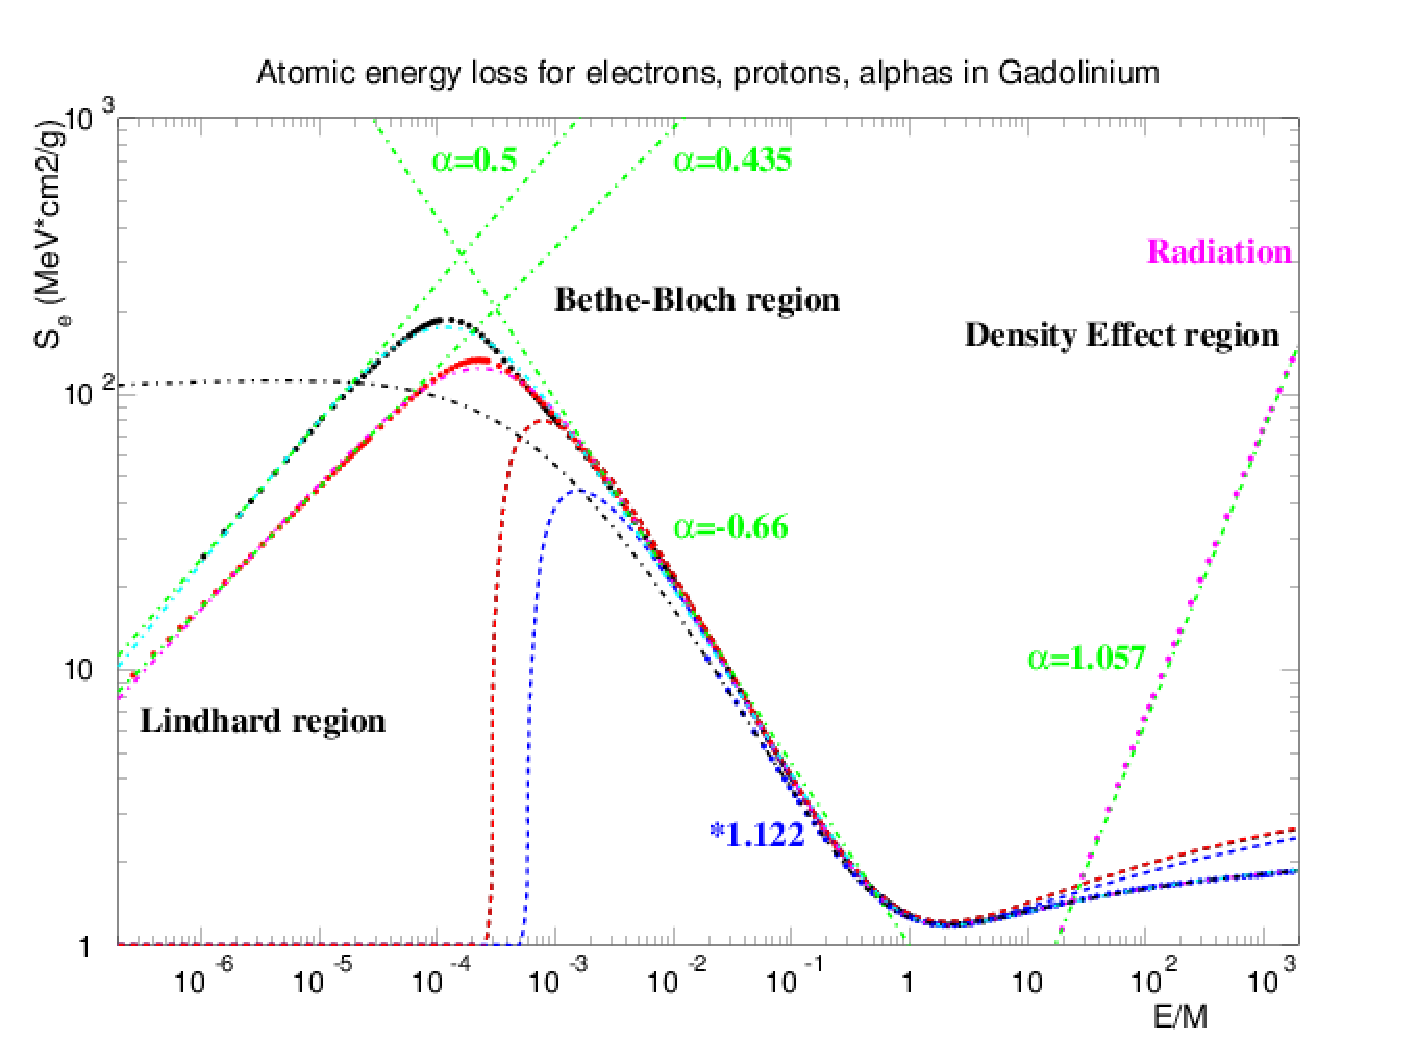
\includegraphics[width=0.99\linewidth]{images/epa_gd_l}
    }
    \caption{Энергетические потери в гадолинии для протонов, $\alpha$-частиц и электронов в зависимости от скейлинговой переменной $y=\frac{E}{M}=\gamma-1$.}
    \label{fig:dEdxGdL}
  \end{figure}
  Для гадолиния на Рис.~\ref{fig:dEdxGdL} показаны аналогичные аппроксимирующие потери энергии электронов, протонов и $\alpha$-частиц.
  Коэффициент нормировки для электронов возрастает до 1.122, то есть приблизительно логарифмически растёт с атомным номером вещества.
  К этой зависимости мы ещё вернёмся.
  В области Линдхарда протоны всё ещё имеют энергетические потери приблизительно пропорциональные скорости, а наклон для $\alpha$-частиц продолжает уменьшаться, то есть наклон для $\alpha$-частиц от углерода до кремния возрастает, а затем снижается при том, что для протонов наклон стабилен.
  В связи с этим возникают существенные систематические ошибки, связанные с расчётом энергетических потерь ионов с большим атомным номером, которые можно рассчитывать от протонов или от $\alpha$-частиц.
  Можно отметить, что ТРТ-кривые (голубая и розовая) на несколько процентов занижают значения энергетических потерь в максимуме ионизации.
  Энергетические потери электронов при малых энергиях приближаются к нормированным энергетическим потерям $\alpha$-частиц в максимуме ионизации, то есть электроны останавливаются резко, поэтому и измерения существуют только до энергии 10 кэВ.
  Это связано с тем, что абсолютная величина как минимальных, так и максимальных энергетических потерь ионов продолжает снижаться.
  
  \begin{figure}[ht]
    {
       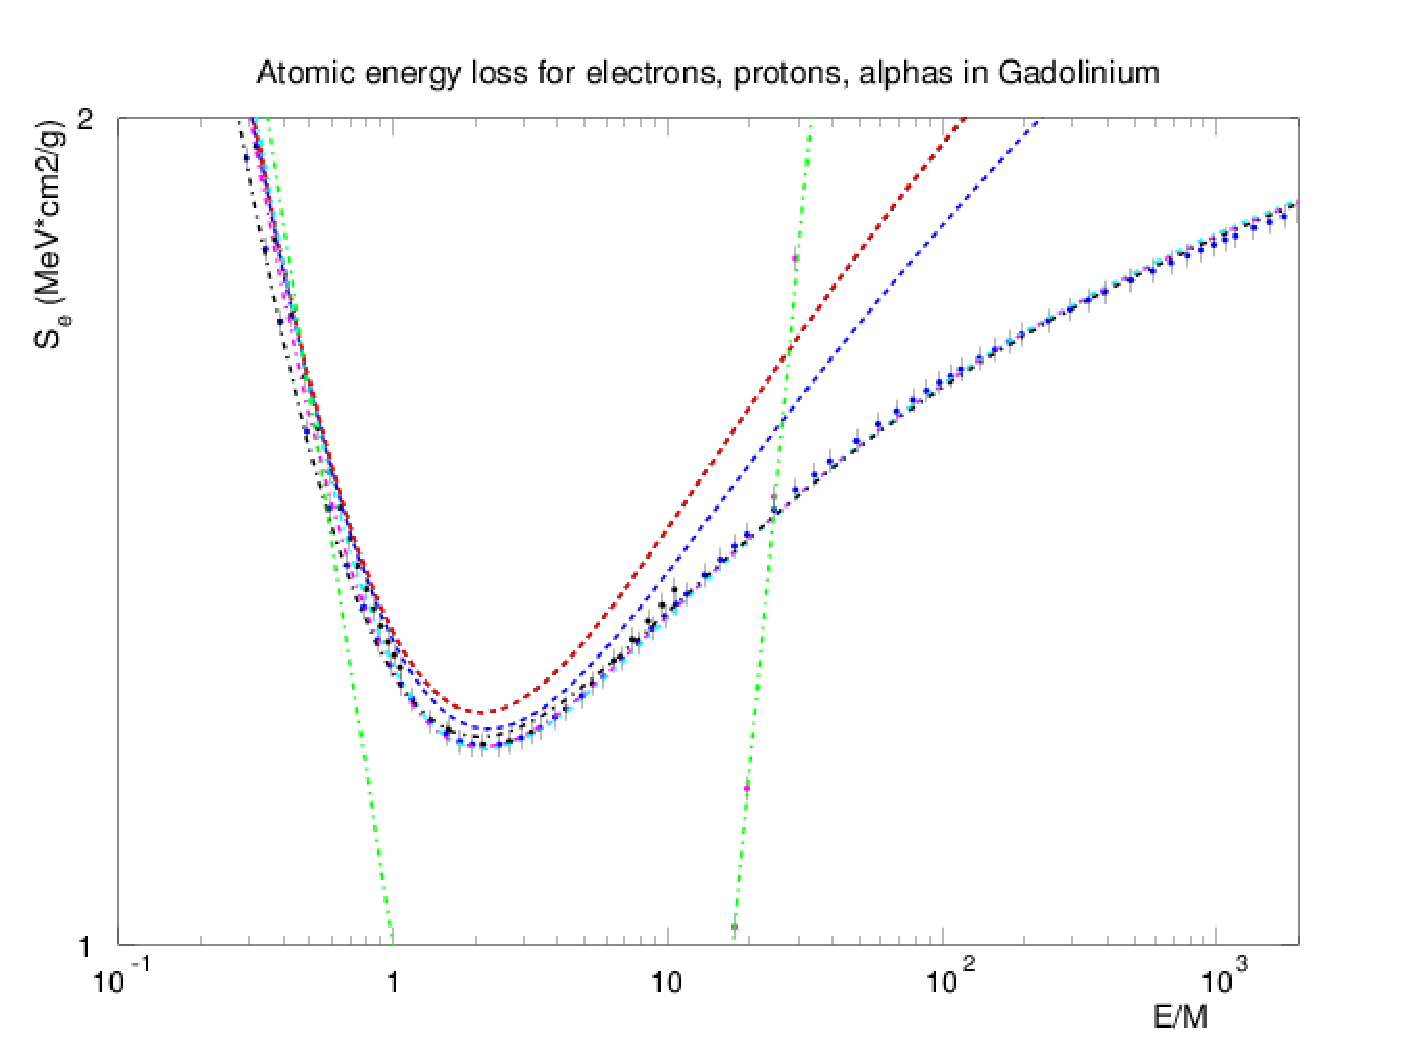
\includegraphics[width=0.99\linewidth]{images/epa_gd_s}
    }
    \caption{Энергетические потери в гадолинии для протонов, $\alpha$-частиц и электронов в области минимальной ионизации.}
    \label{fig:dEdxGdS}
  \end{figure}
  Из Рис.~\ref{fig:dEdxGdS}, построенного в области $y=\frac{E}{M}$ от 0.1 до 2000 для гадолиния, видно, что в области больших $y$ ТРТ кривые для электронов, протонов и $\alpha$-частиц практически совпадают, а электронная (чёрная штрих-пунктирная) кривая идёт выше данных в пределах процента.
  При меньших $y$ она идёт с высокой точностью по аппроксимируемым
   данным.
  Эта неточность связана со сложной зависимостью коэффициента эффекта плотности от энергии, которая будет обсуждаться в отдельном разделе.
  Сложность заключается в том, что форма зависимости коэффициента плотности зависит не только от плотности материала, то есть от агрегатного состояния вещества, но и от плазменной частоты, которая может зависеть от многих условий, в том числе от температуры.
  Тем не менее можно отметить, что ТРТ кривые описывают и электронные и ионные зависимости энергетических потерь даже там, где эти кривые существенно различаются.
  
    \begin{figure}[ht]
    {
       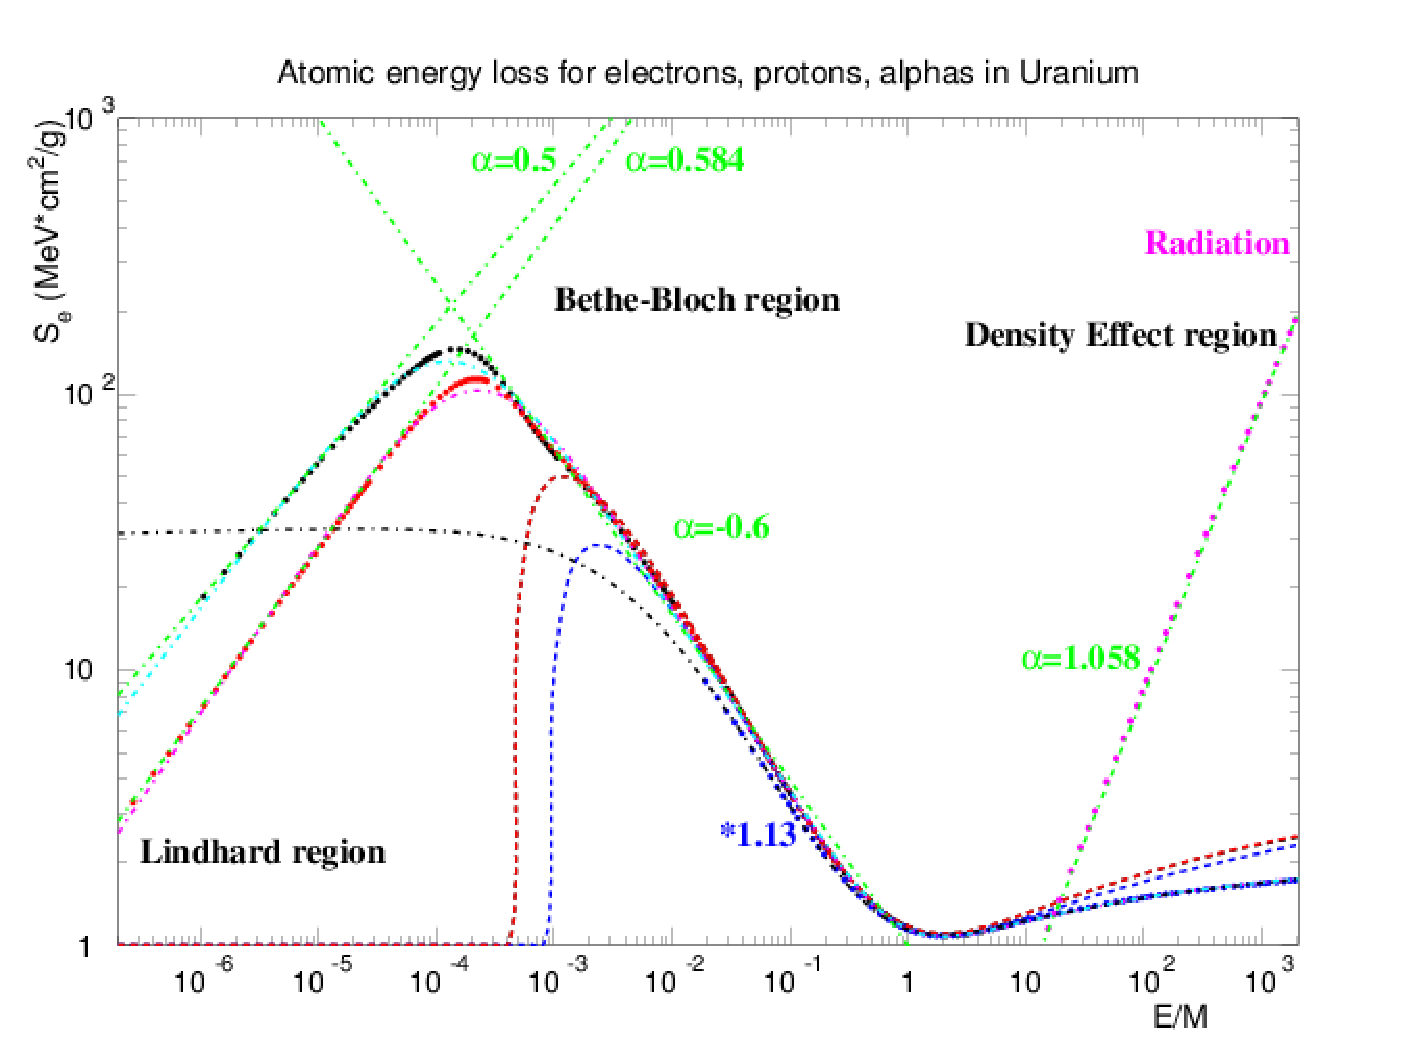
\includegraphics[width=0.99\linewidth]{images/epa_u_l}
    }
    \caption{Энергетические потери в уране для протонов, $\alpha$-частиц и электронов в зависимости от скейлинговой переменной $y=\frac{E}{M}=\gamma-1$.}
    \label{fig:dEdxUL}
  \end{figure}
  Для урана на Рис.~\ref{fig:dEdxUL} показаны аналогичные аппроксимирующие потери энергии электронов, протонов и $\alpha$-частиц.
  Первое, что бросается в глаза в области Линдхарда -- это $\alpha_1=0.584$ для $\alpha$-частиц, которая снова превосходит $0.5$ для протонов.
  Таким образом, показатель $\alpha_1$ для $\alpha$-частиц крайне нерегулярен и колеблется вокруг значения $0.5$.
  По-видимому, эта нерегулярность скажется и на нерегулярности степени роста энергетических потерь при малых энергиях для более тяжёлых жёстких ионов.
  Чтобы решить этот вопрос, необходимо проанализировать большой объём экспериментального материала по энергетическим потерям более тяжёлых ионов.
  Но, Линдхард предсказывал рост со степенью $0.5$ для всех ионов, поэтому, возможно обойтись только наклоном $\frac{C_1}{G}$ линейной по скорости зависимости в формуле (\ref{TPTfitform}).

  \begin{figure}[ht]
    {
       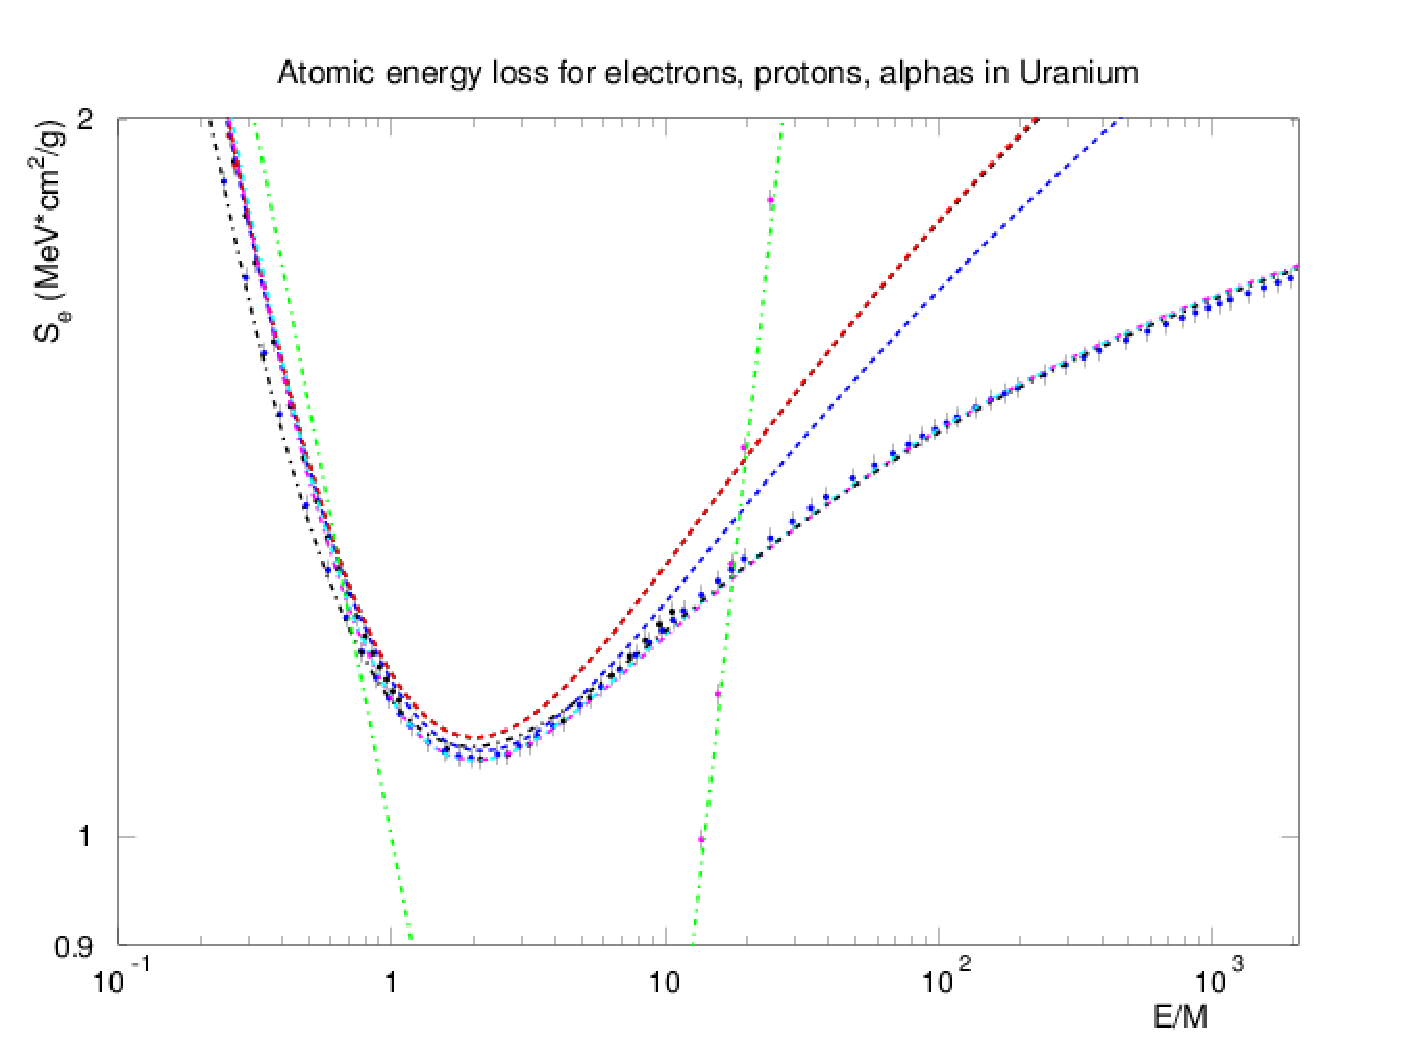
\includegraphics[width=0.99\linewidth]{images/epa_u_s}
    }
    \caption{Энергетические потери в уране для протонов, $\alpha$-частиц и электронов в области минимальной ионизации.}
    \label{fig:dEdxUS}
  \end{figure}
  Из Рис.~\ref{fig:dEdxUS}, построенного в области $y=\frac{E}{M}$ от 0.1 до 2000 для урана, видно, что ТРТ кривые с достаточной точностью аппроксимируют и экстраполируют оцененные данные для урана, приведённые в ASTAR, PSTAR и ESTAR базах данных.
  При этом и электронные, и ионные кривые описываются в области средних энергий с высокой точностью.
  Отметим, что с увеличением атомного веса вещества начало существенного вклада коэффициента эффекта плотности смещается в область б\'{о}льших энергий.
  Можно отметить также, что в области минимума ионизации в уране величина ионизационных потерь равна не 2 МэВ$\cdot$см$^2$/г, как обычно считают, а почти 1 МэВ$\cdot$см$^2$/г, то есть снижение минимальных энергетических потерь несколько снижает эффект увеличения плотности материала при росте его атомного номера.

\subsection{Параметризация эффекта плотности}
\label{dEdx2}

  Коэффициент эффекта плотности $\delta(\beta\gamma)$ в формуле Бете-Блоха (\ref{BetheBloch}) описывает снижение роста энергетических потерь, определяемого первым логарифмическим членом в формуле (\ref{BetheBloch}). Эффект плотности чувствителен не только к агрегатному состоянию вещества, но и к качеству его изготовления, температуре, давлению и т. д. Тем не менее, при нормальных условиях он достаточно хорошо изучен и приводится в базе данных ESTAR.
   Начнём с коэффициента средней энергии ионизации $I$ в формуле (\ref{BetheBloch}).

  \begin{figure}[ht]
    {
       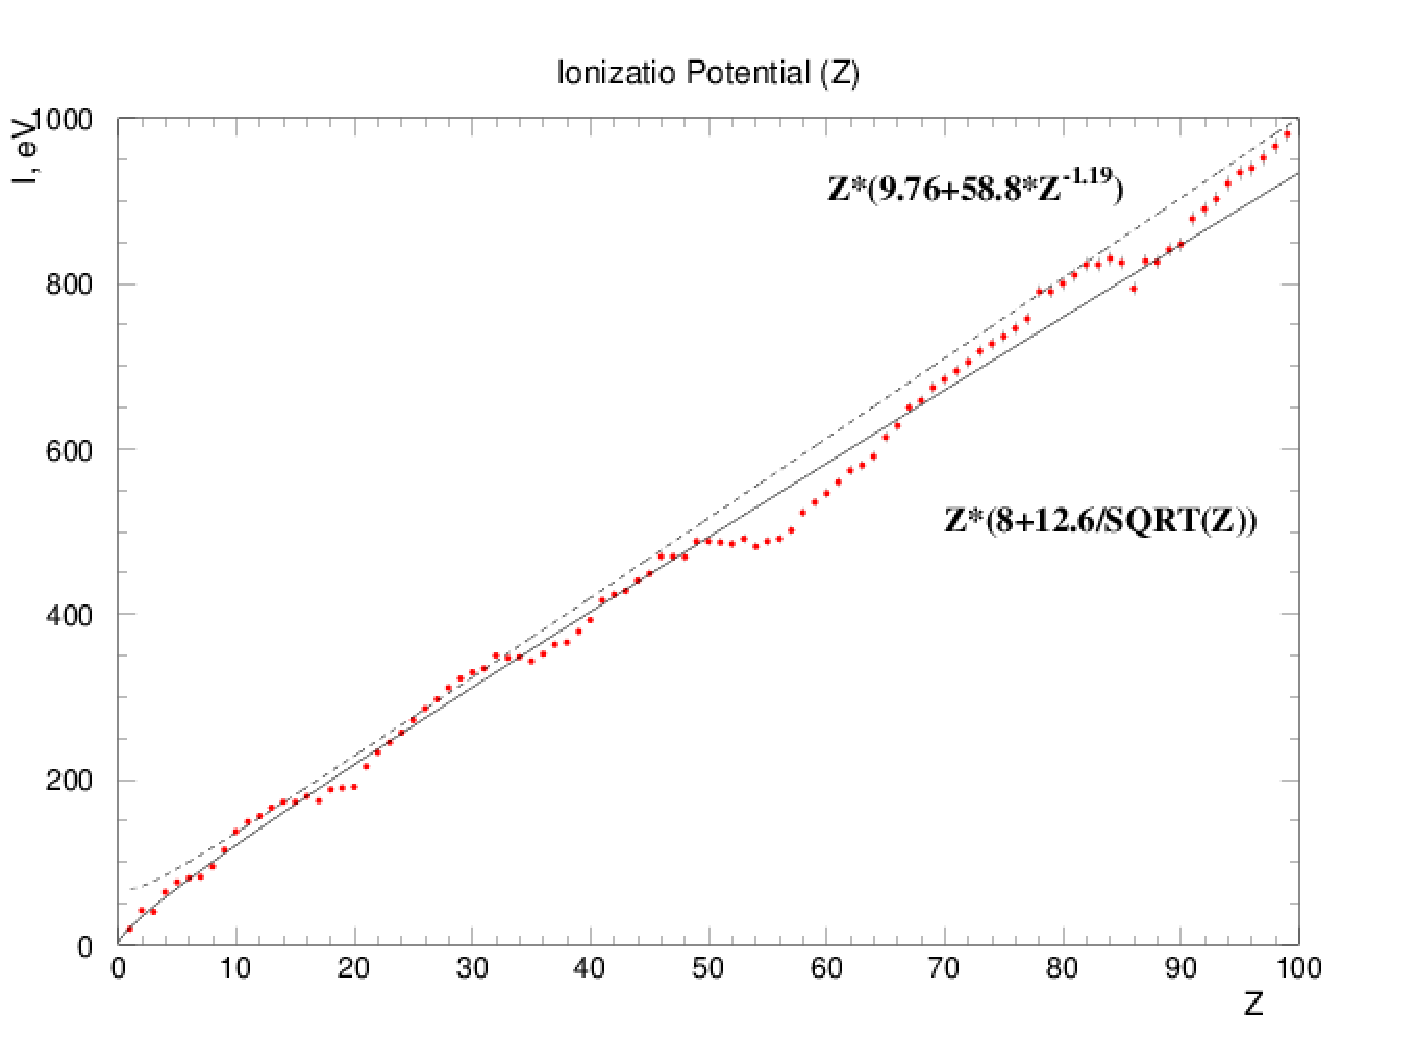
\includegraphics[width=0.99\linewidth]{images/iofz}
    }
    \caption{Зависимость средней энергии ионизации $I$ от атомного номера элемента.}
    \label{fig:iofz}
  \end{figure}
   Они приводятся в базе данных ESTAR для большого набора элементов и материалов и показаны на Рис.~\ref{fig:iofz}.
   Пунктиром проведена стандартная параметризация, используемая в литературе $I=Z\cdot(9.76+58.8\cdot Z^{-1.19})$ (эВ).
   Видно, что, во-первых, эта функция приводит к сингулярности в нуле (показатель степени второго члена отрицателен), а во-вторых, она почти везде идёт выше экспериментальных данных.
   Для материалов из одного элемента можно было бы и не параметризовать $I(Z)$ зависимость, а взять её из таблицы, но для композитных материалов со средним $Z$ нужна формула, максимально  точно описывающая ход $I(Z)$ зависимости.
   Осцилляции, связанные с заполнением оболочек конкретных элементов, в композитных материалах проявляться не будут.
   Сплошной кривой показана ТРТ аппроксимация $I=Z(8+\frac{12.6}{\sqrt{Z}})$, которая очень хорошо описывает потенциалы ионизации в области малых $Z$, характерных для большинства органических веществ.

  \begin{figure}[ht]
    {
       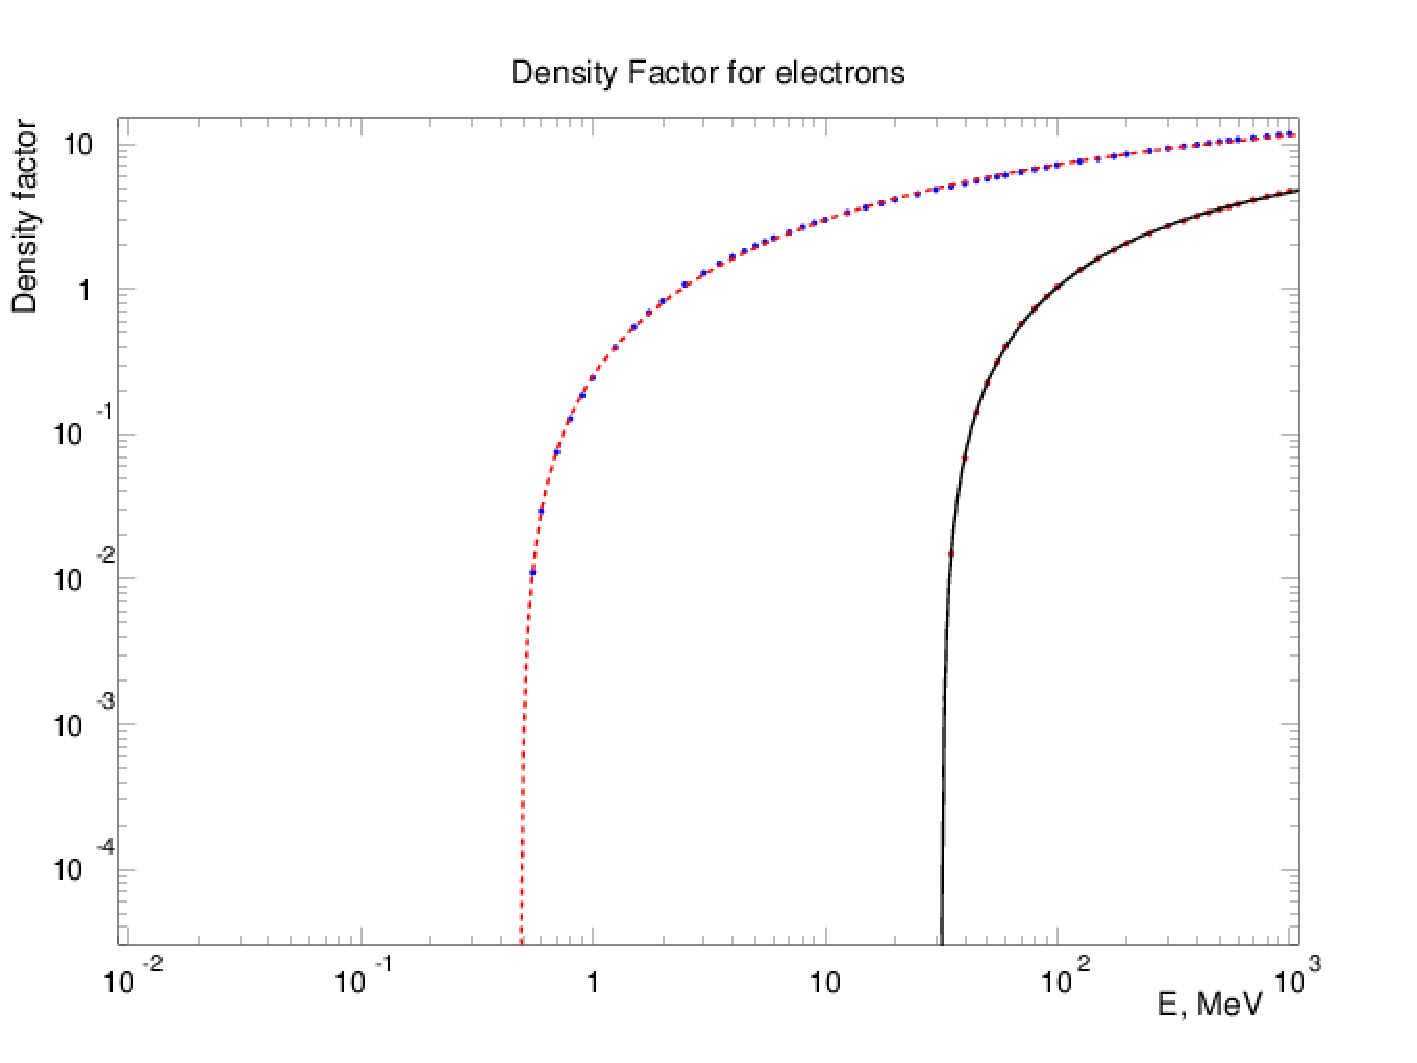
\includegraphics[width=0.99\linewidth]{images/denf_wat}
    }
    \caption{Зависимость эффекта плотности для пара  (красные точки, чёрная ТРТ кривая) и жидкой воды (синие точки, красная пунктирная ТРТ кривая).}
    \label{fig:denf_wat}
  \end{figure}
  На Рис.~\ref{fig:denf_wat} показана энергетическая зависимость эффекта плотности для различных агрегатных состояний воды.
  Видно, что для пара (сплошная чёрная кривая через красные точки, взятые из ESTAR) эффект плотности чувствуется только, начиная с 40 МэВ, а для жидкой воды -- с 0.5 МэВ, причём даже при 1 ГэВ вклад эффекта плотности для воды превосходит эффект плотности для пара почти втрое.
  Была найдена формула, с хорошей точностью описывающая почти все материалы из лёгких элементов, приведенных в ESTAR, и неплохо приближающая функцию даже для тяжёлых элементов:
  \begin{equation}
  \label{DnfApprox}
     \frac{\delta(\beta\gamma)}{2}=\frac{(p_1\cdot\beta\gamma)^{p_2}}{1+(p_3\cdot\beta\gamma)^{p_4}}+\frac{p_5\cdot(ln(\beta\gamma)-p_6)^{p_7}}{1+(p_8\cdot\beta\gamma)^{p_9}}.
  \end{equation}
  Первый член описывает мягкую часть плотных веществ, и он виден только для жидких и твёрдых материалов и, собственно, определяет эффект плотности (для газов он практически отсутствует), а второй член описывает поведение на больших энергиях и существенно зависит от плазменной частоты материала, если считать свободными все электроны материала.
  Для больших энергий все электроны действительно можно рассматривать как свободные, но по мере снижения энергии иона надо учитывать энергию связи электронов.
  
  \begin{figure}[ht]
    {
       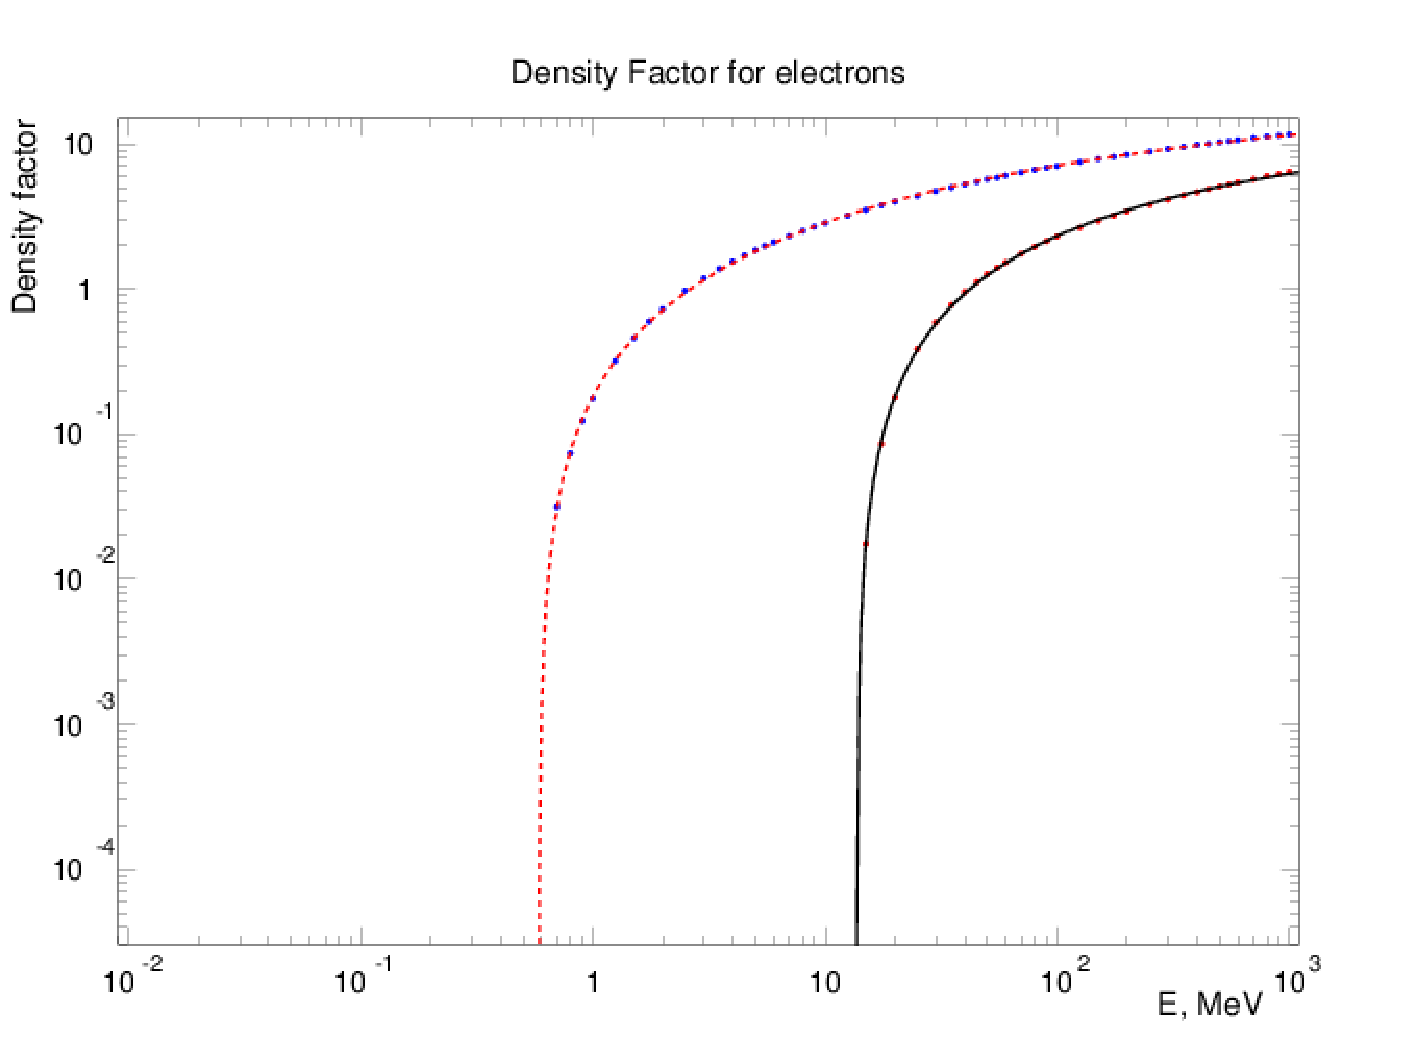
\includegraphics[width=0.99\linewidth]{images/denf_prop}
    }
    \caption{Зависимость эффекта плотности для газообразного пропана (красные точки, чёрная ТРТ кривая) и жидкого пропана (синие точки, красная пунктирная ТРТ кривая).}
    \label{fig:denf_prop}
  \end{figure}
  На Рис.~\ref{fig:denf_prop} то же соотношение эффекта плотности демонстрируется для жидкого и газообразного пропана, хотя при больших энергиях здесь наблюдается меньшее отличие, поскольку молекула длиннее по сравнению с водой.
  Тем не менее можно отметить, что член эффекта плотности для жидкого пропана (синие точки, красная штриховая кривая) появляется при в двадцать раз меньшей энергии, чем для газообразного пропана (красные точки, чёрная сплошная кривая.
  Можно отметить, что для веществ, состоящих в основном из лёгких элементов, а это подавляющее большинство веществ человеческого тела, аппроксимирующая кривая описывает оценочные распределения с высокой точностью.

  \begin{figure}[ht]
    {
       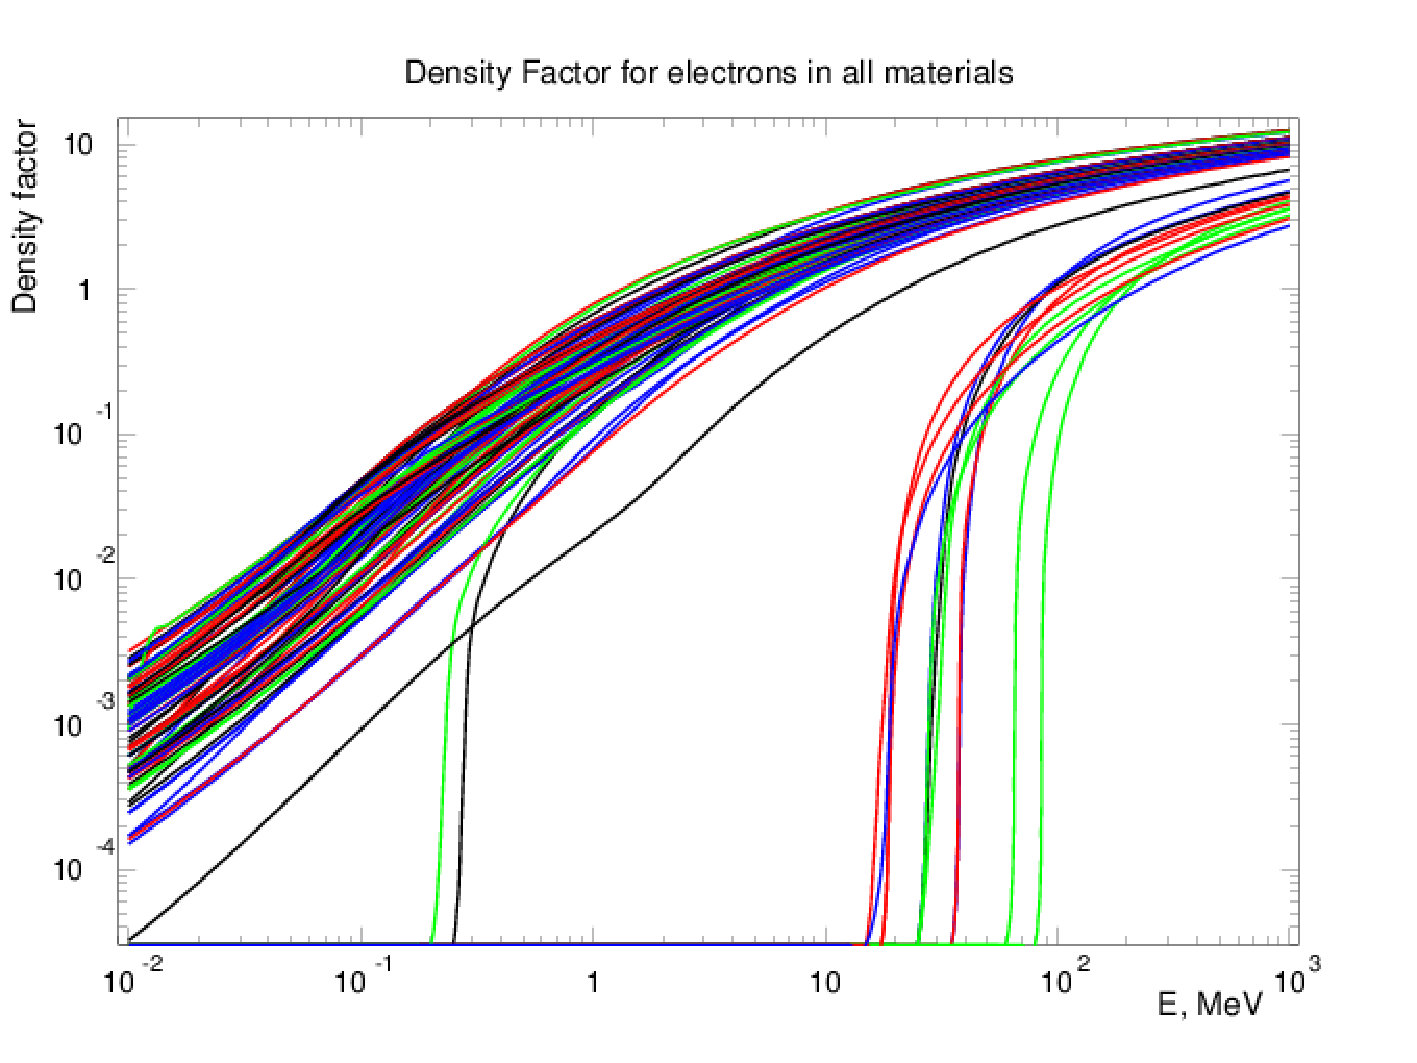
\includegraphics[width=0.99\linewidth]{images/denf_all}
    }
    \caption{Зависимость эффекта плотности для всех моноэлементных материалов базы данных ESTAR.}
    \label{fig:denf_all}
  \end{figure}
  На Рис.~\ref{fig:denf_all} показаны зависимости эффекта плотности для всех материалов базы данных ESTAR, состоящих всего из одного элемента.
  Элементы, эффект плотности для которых начинается после 10 МэВ -- это газы.
  Все элементы, эффект плотности которых начинается до 10 кэВ -- это твёрдые или жидкие вещества
  Особняком стоят вещества, эффект плотности которых начинается при 200-300 кэВ.
  Чёрная кривая соответствует йоду, а зелёная -- астату.
  Это вещества VII группы, неметаллы.
  Их особенностью является растворение в органических веществах, возможно, это и определяет их промежуточное положение.
  Астат крайне редок, а вот для йода этот эффект надо учитывать.
  Самая нижняя кривая из твёрдых веществ соответствует францию, который нестабилен и существует в природе только благодаря $\alpha$-распаду актиния.
  Но, даже если не принимать во внимание этот элемент, разброс твёрдых веществ по интенсивности превосходит порядок величины, то есть эффект плотности -- это крайне индивидуальное свойство материала.
  
  \begin{figure}[ht]
    {
       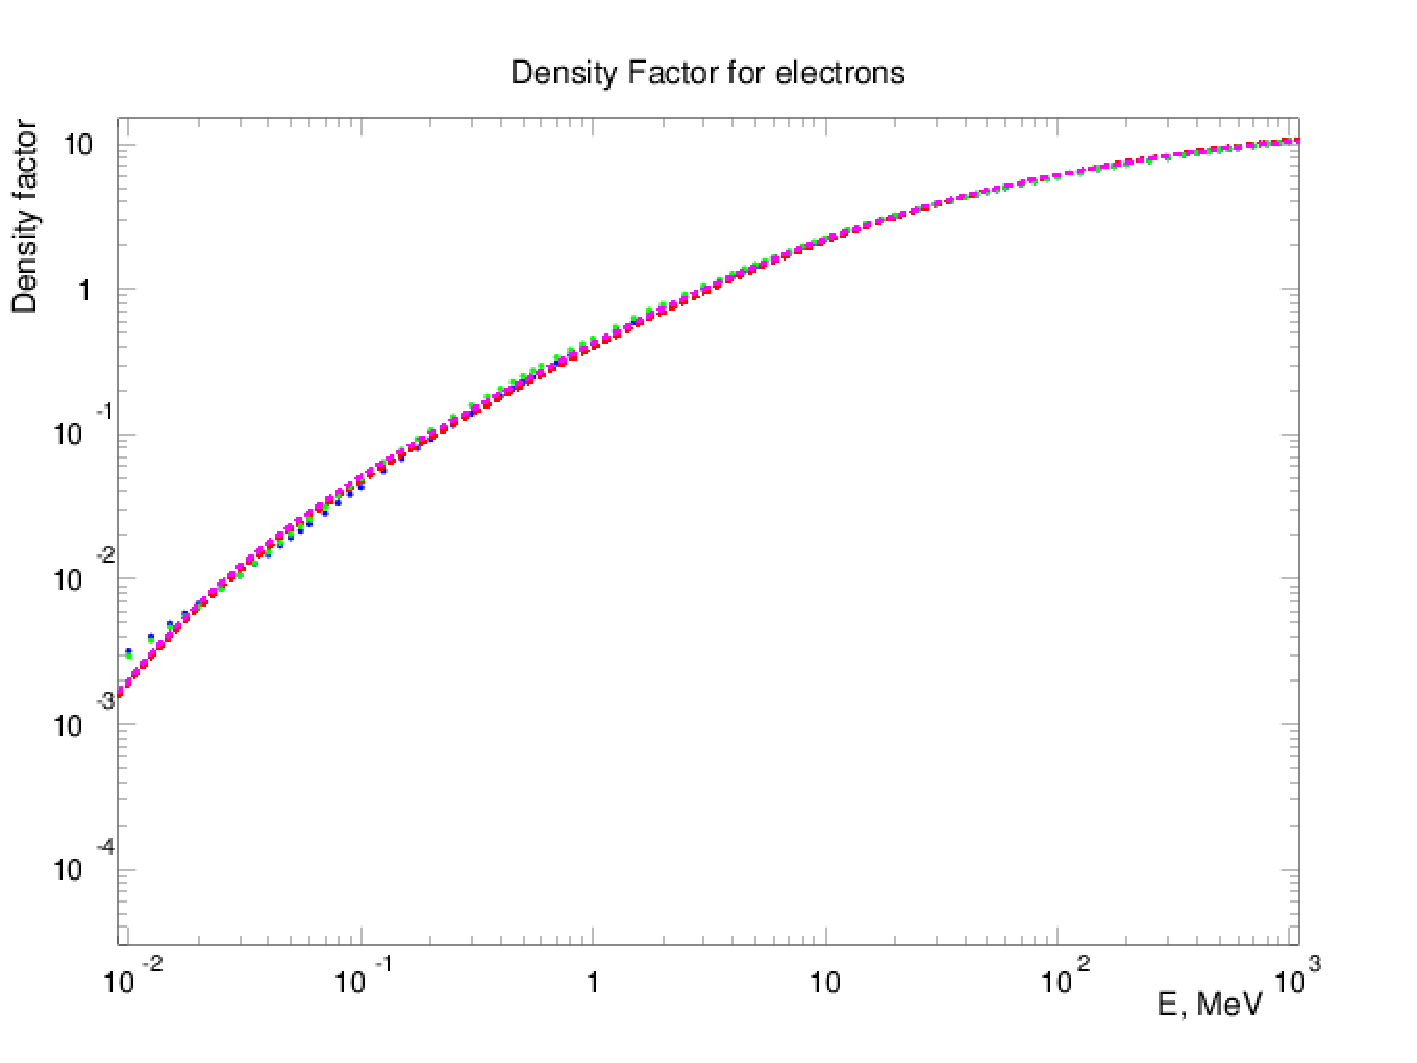
\includegraphics[width=0.99\linewidth]{images/denf_rearth}
    }
    \caption{Эффект плотности для редкоземельных металлов технеций и рутений из базы данных ESTAR.}
    \label{fig:denf_rearth}
  \end{figure}
  На Рис.~\ref{fig:denf_rearth} показаны максимальные эффекты плотности для редкоземельных металлов технеций и рутений.
  Видно, что значения эффекта плотности для редкоземельных металлов продлеваются в область малых энергий с большим значением, чем даёт ТРТ аппроксимация.
  Однако редкие земли практически не встречаются в моделировании ядерных установок в качестве моноэлементного материала, да и величина эффекта плотности при энергиях ниже 20 кэВ ($\frac{E}{M}<0.04$) очень мала.

  \begin{figure}[ht]
    {
       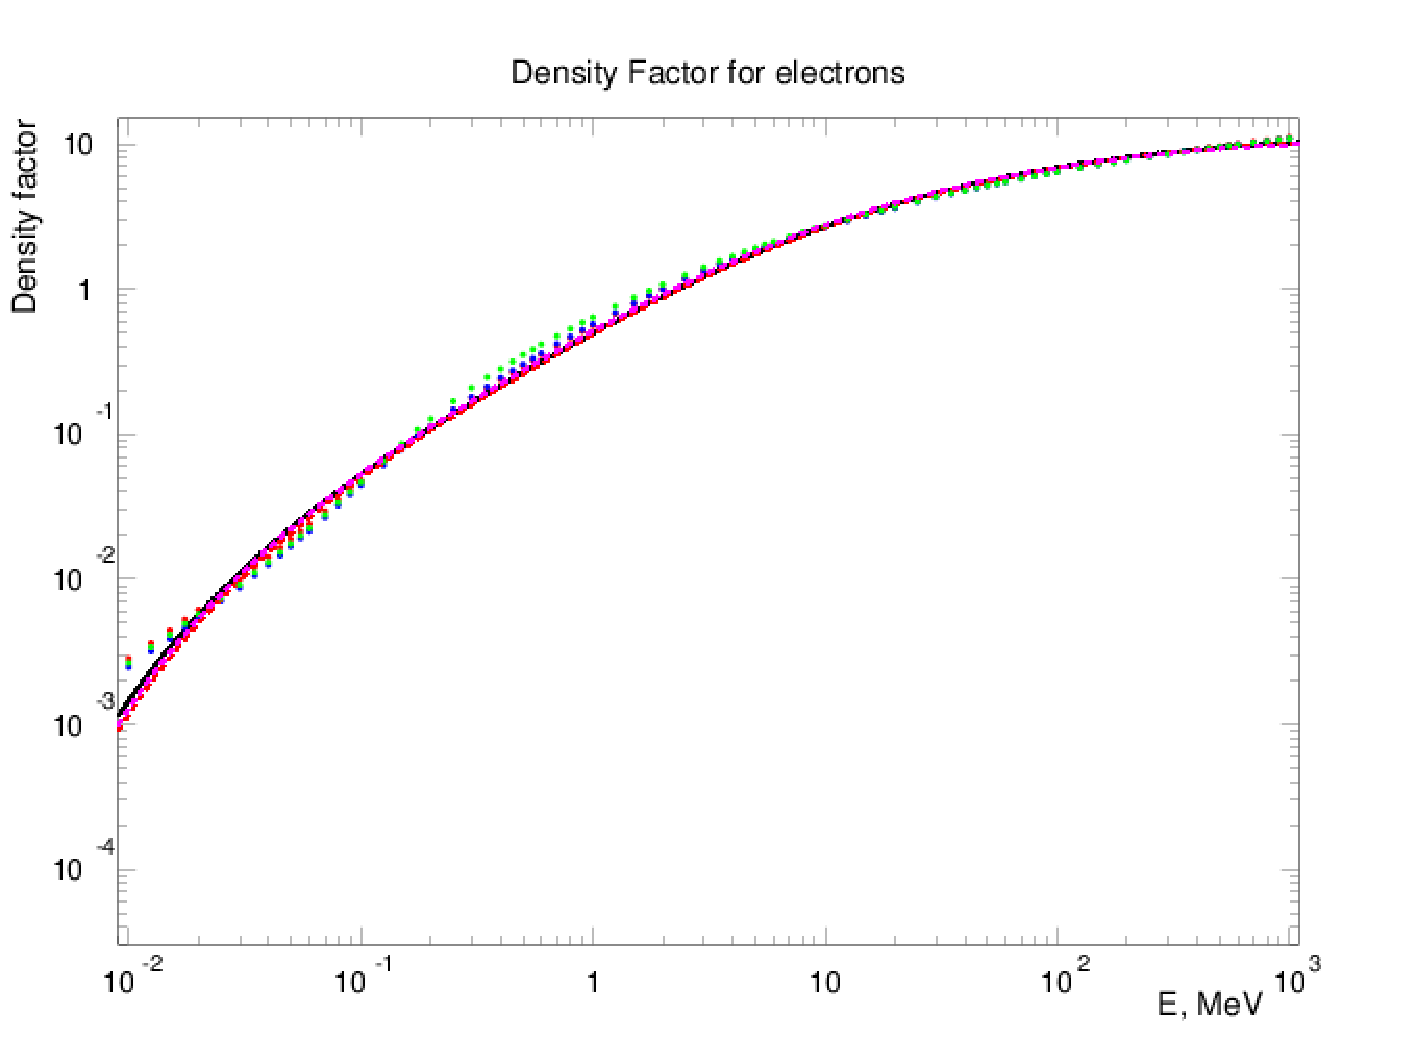
\includegraphics[width=0.99\linewidth]{images/denf_metal}
    }
    \caption{Эффект плотности для металлов железо (синие точки), никель (зелёные точки) и хром (красные точки) из базы данных ESTAR.}
    \label{fig:denf_metal}
  \end{figure}
  На Рис.~\ref{fig:denf_metal} показан эффект плотности для железа, никеля и хрома.
  Видно что и для основных металлов необходимо усовершенствовать аппроксимационную формулу для продолжения оцененных данных (точки) в область малых энергий, если необходимо в точности учесть эффект плотности при этих скоростях.
  Формула вместо таблицы необходима при параллельных расчётах, поскольку напрямую вычислить величину быстрее, чем искать и перекачивать из памяти таблицу для её интерполяции.
  Если взять, скажем $\alpha$-частицы, а не электроны, то согласно скейлингу, энергию электронов надо умножить почти на четыре порядка, что превратит 10 кэВ энергии электрона в 80 МэВ энергии $\alpha$-частицы.
  Практически моделируются $\alpha$-частицы меньших энергий, поэтому вклад эффекта плотности в меньшие энергии надо правильно аппроксимировать.
  С другой стороны, в этой области $\beta\gamma$ для тяжёлых ионов вклад эффекта плотности пренебрежимо мал, поэтому корректное моделирование эффекта плотности может быть важно только для моделирования радиационных разрушений, вызванных космическим излучением, при котором рождаются ионы высокой энергии.

\subsection{Энергетические потери тяжёлых ионов}
\label{dEdx3}

  Приведём теперь эмпирические модели для расчёта энергетических потерь тяжёлых ионов.  
  По Зиглеру доля эффективного заряда тяжелых ионов c зарядом ядра $z$ на ядрах материала с зарядом $Z$:
  \begin{equation}
  \label{GeneralGamma}
  \gamma=q+\frac{C\cdot(1-q)}{2}\cdot\left(\frac{v_0}{v_F}\right)^2\cdot\ln\left[1+\left(\frac{2\Lambda v_F}{a_0v_0}\right)^2\right],
  \end{equation}
 где $v_0=\frac{e^2}{\hbar}$ -- скорость электрона на первой боровской орбите, $a_0$ - радиус первой боровской орбиты, $v_F$ -- скорость ферми в материале, a $q$ - степень ионизации иона вследствие взаимодействия с электронным газом, которая рассчитывается по эмпирической формуле:
   \begin{equation}
  \label{DegreeOfIonisation}
  q=1-\exp(0.803\cdot y_r^{0.3}-1.316\cdot y_r^{0.6}-0.3817\cdot y_r-0.008983\cdot y_r^2),
  \end{equation}
  Эффективная скорость иона $y_r$ вычисляется через скорость иона $v=\sqrt{\frac{2E}{M}}$ ($M$ -- масса налетающего иона) в зависимости от её положения относительно скорости ферми $v_F$.
  Для $v>v_F$:
  \begin{equation}
  \label{effVelocity1}
  y_r=\frac{v}{v_0z^{2/3}}\left(1+\frac{v_F^2}{5\cdot v^2}\right),
  \end{equation}
  а для $v<v_F$
  \begin{equation}
  \label{effVelocity2}
  y_r=\frac{0.75\cdot v_F}{v_0z^{2/3}}\left[1+\frac{2v^2}{3v_F^2}-\frac{1}{15}\left(\frac{v}{v_F}\right)^{4}\right],
  \end{equation}
  которые сшиваются при $v=v_F$.
  $C$ в формуле (\ref{GeneralGamma}) -- множитель второго слагаемого, который корректирует оставшуюся долю заряда вследствие взаимодействия с ядрами материала, поэтому он зависит от заряда ядер материала $Z$:
  \begin{equation}
  \label{CorrFactor}
  C=1+\frac{0.18+0.0015\cdot Z}{z^2}\cdot e^{-7.6+B},
  \end{equation}
  где, как и раньше, $B=\ln(\frac{E}{M})$, $M$ -- это масса и энергия тяжёлого иона-снаряда, а $\Lambda$ -- условная глубина проникновения иона, определяемая формулой:
  \begin{equation}
  \label{ScreeningLength}
  \Lambda=\frac{2\cdot a_0\cdot (1-q)^{2/3}}{z^{2/3}(1-\frac{1-q}{7})}.
  \end{equation}

  Если в формуле (\ref{pseudo-gamma}) вместо $\gamma_\alpha$ подставить значение, рассчитанное по формуле (\ref{GeneralGamma}), то степень ионизации протона можно оценить по формуле $\gamma_p=\frac{\gamma_\alpha}{\gamma}$, где $\gamma$ рассчитана как квадратный корень из выражения (\ref{Hegamma}). Величина $\gamma$, рассчитанная по формуле (\ref{GeneralGamma}) (не путать с кинематической переменной), используется для скейлингового пересчёта энергетических потерь $\alpha$-частицы в энергетические потери тяжёлого иона.

  \subsection{Моделирование упругого ядерного рассеяния иона на ядрах вещества}
  \label{S_nuc}

 Величина ядерного тормозного сечения $S_n$ в единицах эВ$/(10^{15}$ атомов/см$^2)$, для частицы с массой $m$ и энергией $E$ (кэВ) на ядрах вещества с массой ядра $M$ (единицы измерения масс не важны, поскольку они в формулах сокращаются):
  \begin{equation}
  \label{Sn}
  S_n(E)=\frac{8.462\cdot z\cdot Z\cdot m\cdot S_n(\varepsilon)}{(m+M)\cdot(z^{0.23}+Z^{0.23})},
  \end{equation}
  где приведенная энергия $\varepsilon$ рассчитывается как
  \begin{equation}
  \label{epsilon}
  \varepsilon=\frac{32.53\cdot E\cdot M}{z\cdot Z\cdot (m+M)(z^{0.23}+Z^{0.23})},
  \end{equation}
  а масштабно инвариантная функция $S_n(\varepsilon)$ имеет вид.
  \begin{equation}
  \label{SnepsilonLow}
  S_n(\varepsilon)=\frac{\ln(1+1.1383\cdot\varepsilon)}{2\cdot (\varepsilon+0.01321\cdot\varepsilon^{0.21226})+0.19593\cdot\varepsilon^{0.5}}.
  \end{equation}
  При больших энергиях выражение для инвариантной функции упрощается до
  \begin{equation}
  \label{SnepsilonHigh}
  S_n(\varepsilon)=\frac{\ln(\varepsilon)}{2\varepsilon}
  \end{equation}
  Величина ядерного тормозного сечения $S_n$ может быть переведена в единицы МэВ/(мг/см$^2$) умножением на 0.6022/$M$, где $M$ ядра вещества -- в миллиграммах (мг).
  
  В ТРТ мы не используем эти эмпирические формулы, а напрямую используем формулу Резерфорда и суммируем малые энергетические потери в энергию, переданную ядрам вещества на шаге моделирования.
  При этом формула Резерфорда применяется в двух диапазонах по квадрату переданного импульса $|t|$.
  Первый диапазон ограничивается минимальной энергией $W$, которую надо передать атому вещества, чтобы выбить атом из кристаллической решётки.
  Тогда $|t|_{min}$ для дискретного процесса, то есть для процесса с образованием каскадного иона и вакансии можно рассчитать как $|t|_{min}=2W\cdot M$.
  Однако $|t|$ при упругом рассеянии ограничено величиной $|t|_{max}=4p_{CM}^2$, которая соответствует рассеянию назад.
  Величина $p_{CM}^2=\frac{p^2M^2}{s}$, где $p$ -- импульс налетающего иона, а $s$ -- квадрат эффективной массы компаунда в реакции.
  При малых энергиях $s\approx (M+m)^2$, поэтому $|t|_{max}$ при $m<<M$ пропорционален квадрату импульса налетающего иона ($p^2$).
  Если импульс, а значит и энергия, очень малы, тогда пределом интегрирования для рассеяния без выбивания атома из решётки становится $|t|_{max}< |t|_{min}$, а дискретного рассеяния не происходит вовсе.
  Такое Резерфордовское сечение, усечённое величиной $|t|_{min}$ быстро гауссизируется, поскольку отсутствуют ``крылья'', соответствующие рассеянию на большие углы.
  Таким образом, получается ТРТ-модификация многократного рассеяния, дисперсия угла рассеяния которого растёт пропорционально пройденной длине.
  Остаточный дискретный процесс рассеяния на большие углы интегрирует дифференциальное сечение в диапазоне от $|t|_{min}$ до $|t|_{max}$.
  Во-первых, это сечение относительно невелико, поскольку не включает в себя быстро растущую часть дифференциального сечения при $|t| < |t|_{min}$, а во-вторых, включает не только Резерфордовскую (кулоновскую), но и сильную амплитуды.
  Этот вопрос более подробно будет обсуждаться в специальном разделе.
  Энергетические потери, полученные нами с использованием двух этих процессов можно сравнить с эмпирической формулой (\ref{Sn}), используемой в большинстве кодов радиационного транспорта, не ставящих целью описывать радиационную стойкость материалов.

  \subsection{Моделирование процесса многократного рассеяния на ядрах материала.}
  \label{MultipleScattering}

  Заряженная частица при прохождении через вещество испытывает множественные отклонения на малые углы.
  Рассеяние на малые углы происходит главным образом из-за кулоновского рассеяния на ядрах.
  Поэтому эффект изменения угла при прохождении определённой толщины вещества на шаге моделирования называется эффектом многократного кулоновского рассеяния.

  На Рис.~\ref{fig:MultScat} изображено прохождение пучка $\alpha$-частиц через титановую мишень.
  Частицы испускались с расстояния 1 микрометр от поверхности (указано масштабным отрезком). Размеры мишени 3х3х2 мкм.
  На рисунках показаны проекции траекторий, рассчитанные программным комплексом ТРТ, на плоскость XZ (Z вдоль пучка).
  В каждом из пучков с фиксированными энергиями 200 и 600 кэВ разыгрывалось 100 $\alpha$-частиц.

  \begin{figure}[ht]
    {
       \includegraphics[width=0.45\linewidth]{images/alphaInTi_200_keV_100_part}
       \includegraphics[width=0.45\linewidth]{images/alphaInTi_600_keV_100_part}
    }
    \caption{Разброс траекторий $\alpha$-частиц с энергиями 200 кэВ (слева) и 600 кэВ (справа)}
    \label{fig:MultScat}
  \end{figure}

  Из рисунка видно, что, чем выше энергия, тем длиннее область узкого пучка, но по мере того, как ионы замедляются происходит приблизительно одинаковое уширение области остановок ионов.
  При малых энергиях резко возрастает вероятность ион-ионного взаимодействия, отклоняющего частицы на большие углы.
  Для тяжёлых первичных ионов и для тяжёлых материалов это может быть чисто кулоновское однократное рассеяние.
  На левом рисунке видно (почти горизонтальные треки), что иногда такое рассеяние, быстро замедляющее ион, происходит в самом начале пути иона.

 Угол рассеяния при однократном упругом взаимодействии можно рассчитать по формуле:
  \begin{equation}
  \label{CoulombOneScat}
  tg(\theta)=\frac{\Delta p}{p}=\frac{2\cdot z\cdot Z\cdot\alpha}{p\cdot v\cdot b},
  \end{equation}
  где $p$ -- импульс налетающего иона, $v$ -- его скорость, а $b$ -- прицельный параметр реакции.
  Тогда для $n$ последовательных рассеяний:
  \begin{equation}
  \label{CoulombMultScat}
  <\theta^2>=\frac{8\pi\cdot z^2\cdot Z^2\cdot\alpha^2\cdot n\cdot x}{(p\cdot v)^2}\cdot ln\left(\frac{b_{max}}{b_{min}}\right).
  \end{equation}
  Если приравнять $b_{min}$ к радиусу ядра, а $b_{max}$ к радиусу атома, то получим:
\begin{equation}
  \label{CoulombMultLE}
  <\theta^2>=0.157\cdot\frac{z^2\cdot Z(Z+1)\cdot x}{A\cdot(p\cdot v)^2}\cdot ln\left(1130000\frac{Z^{4/3}z^2\cdot x}{A\cdot \beta^2}\right),
\end{equation}
  где $A$ -- атомный вес материала, $x$ в см, $p$ в МэВ, $\beta=\frac{v}{c}$.
  При больших энергиях, когда многократное рассеяние происходит на малые углы, его можно представить в виде вероятностного ($dW=\frac{dN}{N}$, где $dN$ -- число рассеянных частиц, а $N$ -- полное число рассеянных частиц, монитор) углового распределения:
\begin{equation}
  \label{GaussMultHE}
  \frac{dW}{d\Omega}=\frac{1}{2\pi\theta_0^2}\cdot e^{-\frac{\theta^2}{2\theta_0^2}},
\end{equation}
  где дисперсия распределения определяется формулой Бете \cite{Bethe}, параметризованной в работе \cite{Lynch91}:
\begin{equation}
  \label{T0MultHE}
  \theta_0=
  \frac{13.6\cdot z\cdot\sqrt{x/X_0}}{\beta\cdot p}\cdot\left[ 1+0.038\cdot ln\left( \frac{x}{X_0\beta^2}\right)\right],
\end{equation}
в которой $\beta=\frac{v}{c}$, $p$ в МэВ/c, а заряд материала скрыт в величине радиационной длины $X_0$, которая приводится в справочниках для многих материалов.
  Попытка \cite{Scott} улучшить формулу Бете для больших энергий значительно усложняет формулу, но, как было экспериментально доказано \cite{Shen}, не улучшает согласия с экспериментом, поскольку учитывает только электромагнитное рассеяния, а для адронов необходимо учитывать и сильное взаимодействие, приводящее к упругому рассеянию.
  Из-за этого формулы, подогнанные под рассеяние $\mu$-мезонов, не имеющих сильного взаимодействия с ядрами, не работают для сильно взаимодействующих $\pi$-мезонов, и наоборот.

  Для многократного кулоновского рассеяния ионов урана с энергией 650 МэВ/А, рассеянных в медной мишени с толщиной 0,19 радиационной длины, в \cite{Wong} было измерено угловое распределение и сравнено с различными теоретическими формулами.
  Было показано, что для тяжелых ионов хорошо работает простая модель Ферми, изложенная в \cite{Eyges}, поскольку для ионов с большим зарядом в тяжёлом материале ядерным упругим ион-ионным рассеянием можно пренебречь.
  Теория Ферми состоит в том, что в тонком слое складывается множество Томас-Фермиевских рассеяний на малые углы, которое имеет гауссово распределение, и для его среднеквадратичного углового отклонения справедлива формула:
  \begin{equation}
  \label{Fermi}
  \theta^2=\int_0^x T(x') dx',
  \end{equation}
где $T$ -- рассеивающая способность (scattering power), которая ещё раньше была вычислена для космических лучей \cite{RossiGreisen}:
  \begin{equation}
  \label{Rossi}
  T=\frac{2\pi\cdot m_e^2}{\alpha\cdot X_0}\cdot\left(\frac{z}{pv}\right)^2.
  \end{equation}
  В последние годы в связи с развитием медицинского направления ионной терапии возникла новая японская технология расчёта среднего угла многократного рассеяния в тонком слое.
  Она основана не на каких-то определённых потенциалах ион-ионного взаимодействия, а на анализе огромного количества экспериментальных данных, как для лёгких материалов и лёгких ионов, так и для тяжёлых материалов и тяжёлых ионов \cite{Wong}.
  Опуская все промежуточные приближения, величина среднеквадратичного угла отклонения в тонком слое была рассчитана в \cite{Kanematsu9}  в виде:
  \begin{equation}
  \label{Kane9}
  <\theta^2>=10^{-3}z^{-0.16}A^{-0.92}\cdot\frac{X_0^{wat}}{\rho_s\cdot X_0^{mat}}\cdot ln\left(\frac{R_0}{R_0-\rho_s\cdot x}\right),
  \end{equation}
где $X_0^{wat}$ -- радиационная длина для воды, а $X_0^{mat}$ -- радиационная длина материала мишени, $\rho_s$ -- относительный темп энергетических потерь $\rho_s=\left(\frac{dE}{x}^{mat}/\frac{dE}{x}^{wat}\right)$, $R_0$ -- пробег иона до остановки в воде.
  Используя в качестве базового процесса процесс многократного рассеяния в воде, можно, с одной стороны, избавиться от логарифмических поправочных факторов, а с другой -- привязаться к очень хорошо изученным функциям для воды, поскольку вода -- основной материал человеческого тела, и поэтому наиболее хорошо изучена.
  Подход тонких слоёв, предложенный и реализованный в ТРТ, позволяет существенно упростить эту зависимость в пределе тонкого слоя ($x\longrightarrow 0$):
  \begin{equation}
  \label{KaneTPT}
  <\theta^2>=10^{-3}z^{-0.16}A^{-0.92}\cdot\frac{X_0^{wat}}{X_0^{mat}}\cdot \frac{x}{R_0}.
  \end{equation}
  Величины $X_0^{wat}$ и $X_0^{mat}$ приводятся в таблицах, а величина $R_0$ рассчитывается из формул ионного скейлинга, исходя из PSTAR и ASTAR таблиц, которые именно для воды измерены с высочайшей точностью.
  Однако надо иметь в виду, что факторизация многократного рассеяния, связанная с выделением процесса рассеяния на большие углы, может потребовать модернизации, как самих PSTAR и ASTAR таблиц, так и формул ионного скейлинга.
  Но это уже будут поправки второго порядка.

  Новая японская технология, развитая в последние годы и использованная в программном комплексе ТРТ, пока не использована в таких известных кодах как MCNP и Geant4, поскольку в MCNP торможение ионов всегда рассматривались как локальный эффект второго порядка, а в Geant4 упор был сделан на высокие энергии, и развитие физики для ионной терапии всегда рассматривалась как второстепенная задача.
  В любом случае разделение процесса многократного рассеяния на ядерную и электромагнитную части в обоих кодах было затруднено, поскольку электромагнитной и ядерной физикой всегда занимались разные группы разработчиков.
  Это позволяет надеяться, что какое-то время TPT будет уникальной программой способной в эксклюзивном режиме моделировать транспорт ионов и ионные каскады в мишенях.

\clearpage
\section{TPT моделирование ион-ионного ядерного упругого рассеяния.}
\label{Pol}

	Моделирование упругого рассеяния в полном объёме реализовано в программном комплексе ТРТ для нейтронов, причём, в отличие от других программ температурная зависимость сечения упругого рассеяния реализована не таблично, как в MCNP, и не путём Монте-Карло расчёта, как в Geant4, а аналитически.
	Рассеяние протонов будет реализоваться по тому же алгоритму.
	Единственным принципиальным отличием будет то, что нейтронное упругое сечение достигает самых малых энергий, где из-за усреднения по скорости реакции оно начинает зависеть от температуры материала \cite{70/190-T}, а протонное сечение вследствие кулоновского барьера (фактора Гамова) быстро падает к нулю энергии, поэтому от температуры практически не зависит, что упрощает моделирование.
	С другой стороны, дифференциальные угловые сечения упругого рассеяния для протонов изучены значительно более детально, поскольку для заряженных частиц возможна спектрометрическая методика.
	В этом смысле более точная модель упругого протон-ядерного рассеяния может помочь модернизировать модель упругого нейтрон-ядерного рассеяния, которое в данный момент базируется на экспериментальных данных относительно низкой точности.
	В частности, исходя из микроскопических моделей можно связать дифференциальные угловые сечения для упругого рассеяния протонов и нейтронов в зеркальных реакциях.
	Возможно, выделяя изотопически-асимметричный ядерный кор, можно будет продвинуться и выше по дорожке стабильности.
	Эту программу теоретического уточнения сечений упругого рассеяния нейтронов с использованием данных об упругом рассеянии протонов можно рассматривать в качестве ростковой точки для модернизации программного комплекса ТРТ.

	С другой стороны, микроскопическая модель резонирующих групп, развиваемая в ЦФПИ ВНИИА (АВМРГ -- один из вариантов алгебраических кластерных моделей), позволяет описывать ядерные взаимодействия на относительно больших расстояниях, то есть с относительно большими орбитальными моментами по сравнению с моделью ядерных оболочек.
	В частности, для лёгких ядер-мишеней уже была продемонстрирована возможность расчёта фаз рассеяния лёгких заряженных ионов \cite{IgashSol17}.
	Принципиально эта методика расчёта ограничена фазами рассеяния для одного-двух нижних орбитальных моментов, но больше при низких энергиях и не нужно, поскольку во вкладе более высоких фаз, дающих вклад в рассеяние на малые углы, доминируют кулоновские члены, и они уже учтены в многократном рассеянии, эффективно учитывающем электронную экранировку заряда ядра электронами путём аппроксимации экспериментальных данных, как это было обсуждено в предыдущем разделе, а не путём теоретического расчёта, который даёт описание лишь на качественном уровне и обычно далёк от экспериментальных данных.
	Качество описания упругих сечений моделью АВМРГ было продемонстрировано в отчёте прошлого года \cite{70/662-T}.
	Отметим, что в программном комплексе ТРТ найдено решение, которое не могли найти разработчики других программ.
	Всегда хотелось как-то разделить вклад электромагнитных и ядерных амплитуд.
	Поскольку электромагнитное рассеяние даёт вклад главным образом в рассеяние на малые углы, а упругое ядерное рассеяние -- на большие углы, пытались поставить границу по углу рассеяния $\theta$, но это релятивистски неинвариантное решение не даёт желаемого результата.
	Тогда было предложено провести границу между электромагнитным и ядерным рассеянием по релятивистской Мандельстамовской переменой переменной $|t|$, которая при низких энергиях сводится к величине $2p^2(1-cos(\theta))$ ($p$ --импульс налетающего иона), а в пределе малых углов сводится к $p^2\cdot\theta^2$, то есть к квадрату поперечного переданного импульса.
	Но и этот вариант оказался неудовлетворительным, поскольку дифракционный конус ядерного рассеяния даёт существенный вклад в рассеяние на малые углы, а электромагнитное рассеяние при малых прицельных параметрах способно приводить к рассеянию на большие углы, что хорошо известно специалистам по поверхностному LEIS анализу.
	Эта проблема усугубляется с ростом зарядов налетающего иона и иона-мишени.

	В программном комплексе ТРТ найден универсальный способ корректного учёта и ядерных, и электромагнитных взаимодействий.
	Разграничение производится не по релятивистски-инвариантной переменной $|t|$, а по первым фазам рассеяния.
	На модельном уровне считаются первые фазы, которые условно соответствуют малым прицельным параметрам и включают в себя, как ядерные (адронные), так и электромагнитные вклады, позволяющие одновременно учесть и ядерное и электромагнитное рассеяние на большие углы.
	Старшие фазы, соответствующие большим орбитальным моментам и малым прицельным параметрам, которые определяют большую вероятность рассеяния на малые углы, вовсе не вычисляются, а считаются учтёнными в эффективном дискретном процессе многократного рассеяния в тонком слое.
	Это разделение позволяет, с одной стороны, проводить теоретический расчёт с достаточно малыми толщинами, а с другой стороны позволяет использовать фазы, которые экспериментаторы извлекают из дифференциальных угловых сечений упругого рассеяния, и использовать их для моделирования конкретных ионов в конкретных материалах, соответствующих экспериментально измеренным ион-ионным парам.
	Альтернативным подходом является новый предложенный в ТРТ метод, основанный на полуэмпирической Теории Прямых Реакций (ТПР).

	Заметим, что дискретное упругое рассеяние энергичного иона на ядрах мишени производится эксклюзивно, то есть в конечном состоянии возникает два иона: рассеянный энергичный ион-снаряд и ядро отдачи.
	При этом сохраняется энергия и импульс, что делается не во всех кодах, где иногда переданную ядру отдачи энергию просто записывают в потерянную энергию, и дальнейший транспорт ядра отдачи не производится.
	Это, в частности, оправдывается тем, что при многократном рассеянии, когда импульс передаётся большому числу ядер, ядра получают столь малую энергию, что им не удаётся далеко удалиться от места выбивания в твёрдом теле, и малая переданная им энергия передаётся фононам твёрдого тела, то есть приводит просто к нагреву мишени.
	При таком моделировании разрушение материала вообще не учитывается.
	Уточняя эту логику, процесс ион-ионного рассеяния разбивается на две части: события, в которых ядро отдачи транспортируется в твёрдом теле, что соответствует процессу упругого ион-ионного рассеяния, и события, когда ядра отдачи не транспортируются, поскольку остаются на месте, и переданная им энергия приводит лишь к нагреву, -- этот процесс, всё же изменяющий направление движения падающего иона, даёт вклад в многократное рассеяние.
	При ТРТ моделировании, как было показано, малую переданную частице мишени энергию прибавляют к электронным энергетическим потерям.
	Таким образом, выделяемая в процессе многократного рассеяния энергия учитывается в непрерывной функции энергетических потерь иона на шаге моделирования.
	Непрерывным называется процесс, который происходит не в конце шага моделирования, что характерно для дискретных процессов, а процесс передачи веществу и иону энергии и импульса, пропорциональных длине шага моделирования.
	В программе по значению энергии, заряду, и массе иона определяется темп энергетических потерь иона $\frac{dE}{dx}$ и умножается на длину шага моделирования $\Delta L_i$ на $i$-м шаге, так что $\Delta E_i=\frac{dE}{dx}\cdot\Delta L_i$.
	Потери энергии складываются из ионизационных и из неионизационных потерь.
	Малые энергетические потери при многократном рассеянии относятся к неионизационным потерям.

\subsection{Многократное рассеяние при прохождении ионов низкой энергии через тонкие слои дейтерида титана}
\label{subPol2}

  Обычно при моделировании многократного рассеяния ионов в веществе предполагается, что оно имеет гауссово угловое распределение.
  Однако экспериментально известно, что у реального углового распределения имеются ``хвосты'', которые распределением Гаусса не описываются и, чем меньше пробег ионов в веществе, тем больше угловое распределение многократного рассеяния отличается от гауссова (тем больше ``хвосты'').
  Использование распределения Гаусса для описания углового распределения многократного рассеяния предполагает, что пробег частиц в веществе достаточно велик для того, чтобы их распределение по углу рассеяния успело ``гауссизироваться'', т. е. накладывается ограничение снизу на шаг моделирования.
  В численном эксперименте мы обнаружили, что при совсем малых шагах надо учитывать не только ``хвосты'', но и узкий пик в нуле (``нос'').
  Наличие ``хвоста'' и ``носа'' обусловлено тем, что Резерфордовское рассеяние имеет вид функции $\frac{1}{t^2}$, которое имеет более узкий, чем гауссово распределение ($e^{-At^2}$), максимум вперёд (обуславливающий появление ``носа'') и более медленное, чем гауссово распределение, падение при больших $|t|$ (обуславливающее появление ``хвоста'').
  Цель численного моделирования состоит в том, чтобы описать ``нос'' и ``хвост'' углового распределения многократного рассеяния при прохождении ионов через тонкие слои вещества.
  Это позволит учитывать влияние многократного рассеяния начиная с очень малых длин пробега ионов в веществе, то есть для очень малых шагов моделирования, которые необходимы при описании ионных каскадов, индуцированных потоком нейтронов.

  В ходе моделирования мишень из дейтерида титана бомбардировалась ядрами дейтерия.
  Мишень была разделена на 32 слоя, при прохождении дейтронов через каждый из которых можно было строить гистограмму функции плотности вероятности углового распределения многократного рассеяния и следить за её изменением и изменением других параметров (средняя кинетическая энергия ионов и её дисперсия, средняя накопленная потеря энергии ионами за счёт $\frac{dE}{dx}$ вещества и др.) от слоя к слою.
  Это давало возможность на слоях, соответствующих малым толщинам, увидеть и аппроксимировать ``нос'' (более узкое гауссово распределение) и ``хвост'' (более широкое гауссово распределение) углового распределения многократного рассеяния, определяемые многократным Резерфордовским рассеянием.
  Изменением параметра толщины слоя можно было изменять толщину моделируемой мишени. 

  В кристаллической решётке дейтерида титана энергия, необходимая для выбивания ионов титана и дейтерия из их равновесного положения в узлах решётки (так называемая ``displacement energy'') $E_{de}$, равняется примерно 25 эВ для титана и примерно 10 эВ для дейтерия.
  Эти значения используются, например, в программе SRIM \cite{SRIM}, применяющейся для моделирования ионного транспорта, и программах молекулярной динамики.
  Так как при кинетической энергии налетающей частицы, меньшей указанных значений, не происходит выбивания иона дейтерия либо титана из их равновесного положения в узле кристаллической решётки в результате Резерфордовского рассеяния, можно в качестве дифференциального сечения $\frac{d\sigma}{d|t|}$ многократного рассеяния рассматривать дифференциальное сечение Резерфордовского рассеяния при $|t|$ от 0 до
\begin{equation}
\begin{aligned} 
 \label{MSTmin}  
    |t|_{min}=2E_{de}M
\end{aligned}
\end{equation}
(в формуле (\ref{Xp}) вместо кинетической энергии ядра отдачи подставляется величина $E_{de}$), где $M$ -- масса ядра мишени, а значение $E_{de}$ берётся либо для дейтерия, либо для титана, в зависимости от того, на каком ядре рассеивается налетающая частица.
  При $|t|>|t|_{min}$ можно рассматривать полное дифференциальное сечение упругого рассеяния, являющееся интерференцией электромагнитной (Резерфордовской) и ядерной амплитуд рассеяния.
  При этом, так как Резерфордовское дифференциальное сечение рассеяния различных частиц, определяющееся выражением (\ref{Dimension1p}), неограниченно растёт при $|t| \to 0$, для того, чтобы полное сечение, являющееся интегралом от дифференциального сечения, сходилось, необходимо учитывать постоянную электронной экранировки $A_S$, делающую $\frac{d\sigma}{d|t|}$ конечным при $|t| \to 0$ ($\theta_{CM} \to 0$, $\theta_{LS} \to 0$):
\begin{equation}
 \begin{aligned} 
 \label{MS1}     
      \frac{d\sigma}{d|t|}=  
      \frac{A_R^2}{\left( |t| + 4 p_{CM}^2 A_S \right)^2} \cdot \left( \hbar c \right)^2,
 \end{aligned}
\end{equation}
где согласно \cite{G4IonIon}:
\begin{equation}
\label{MSAs}
\begin{aligned} 
A_S= \left( \frac{ \hbar }{ 2 p_{CM} a_L } \right)^2 \cdot \left( 1.13 + 3.76 \cdot \left( \frac{ \alpha z Z}{\beta_{CM}} \right)^2 \right).
\end{aligned}
\end{equation}

Здесь $p_{CM}$ -- импульс в системе центра масс, радиус электронной экранировки определяется выражением, рассчитанным в \cite{LinhardScreeningLength}:
\begin{equation}
\label{MSaL}
\begin{aligned} 
a_L=\frac{ C_{TF} \cdot a_0 }{ \left( z^{2/3} + Z^{2/3} \right) },
\end{aligned}
\end{equation} 
где $C_{TF}= \frac{1}{2} \left( \frac{3\pi}{4} \right)^{2/3}$ -- постоянная электронной экранировки Томаса-Ферми \cite{ThomasFermiModel}, $a_0=\frac{ \hbar^2 }{ m_ee^2 }$ -- боровский радиус, $m_e$ -- масса электрона, $z$ и $Z$ -- заряды налетающей частицы и мишени, $\beta_{CM}=\frac{p_{CM}}{E_{CM}^{\mu}}$ -- скорость приведённой частицы в системе центра масс ($c=1$), а энергия приведённой частицы в системе центра масс $E_{CM}^{\mu}=\sqrt{p_{CM}^2+\mu^2}$, где приведённая масса $\mu=\frac{mM}{m+M}$ и $m$ -- масса покоя налетающей частицы, $M$ -- масса покоя ядра-мишени.

Прежде чем перейти к вычислению сечения многократного рассеяния, необходимо упомянуть, что переменная $|t|$ ограничена сверху значением (\ref{Tmax}),
соответствующим рассеянию в системе центра масс на максимальный угол $\theta_{CM}=\pi$ (см. (\ref{Xp})). Тогда верхний предел интегрирования выражения (\ref{MS1}), необходимый для вычисления интегрального сечения многократного рассеяния, можно определить как величину $|t|_m$, равную $|t|_m=|t|_{max}$, если $|t|_{max}<|t|_{min}$, и $|t|_m=|t|_{min}$, если $|t|_{max} \geq |t|_{min}$.

Сечение многократного рассеяния в переднюю полусферу можно тогда определить как
\begin{equation}
\label{MSSigmaFull} 
\sigma^*_{ms}= \int \limits_0^{|t_{m}|} \frac{\left( \hbar c \right)^2 A_R^2 d|t|}{\left( |t| + 4p_{CM}^2 A_S \right)^2} = \left( \frac{\mu \alpha z Z \hbar c }{2p_{CM}^2} \right)^2 \frac{\pi\frac{|t_{m}|}{p_{CM}^2}}{ A_S \left( \frac{|t_{m}|}{4p_{CM}^2} + A_S \right) }.
\end{equation}

Выражение (\ref{MSSigmaFull}) справедливо для рассеяния различных частиц ($D-Ti$, $Ti-D$ и т. п.). В случае рассеяния тождественных частиц ($p-p$, $D-D$, $Ti-Ti$ и т. п.), когда дифференциальное сечение $\frac{d\sigma}{d|t|}$ симметрично относительно $|t|=2p_{CM}^2$, соответствующего углу рассеяния в системе центра масс $\frac{\pi}{2}$, формула (\ref{MSSigmaFull}) принимает вид
\begin{multline}
\label{MSSigmaFullEqual}
%\begin{aligned} 
\sigma_{ms}= \left( \hbar c \right)^2  A_R^2 \left( \int \limits_0^{|t_{m}|} \frac{d|t|}{\left( |t| + 4p_{CM}^2 A_S \right)^2} + \int \limits_{|t_{max}|-|t_m|}^{|t_{max}|} \frac{d|t|}{\left( |t| + 4p_{CM}^2 A_S \right)^2} \right)= \\ \left( \frac{\mu \alpha z Z \hbar c }{2p_{CM}^2} \right)^2 \frac{2\pi\frac{|t_{m}|}{p_{CM}^2}}{ A_S \left( \frac{|t|_{m}}{4p_{CM}^2} + A_S \right)} = 2 \sigma^*_{ms}.
%\end{aligned}
\end{multline}

  В процессе моделирования при использовании формулы (\ref{MSSigmaFull}) для описания сечения многократного рассеяния дейтрона на ядре титана и (\ref{MSSigmaFullEqual}) -- дейтрона на дейтроне, вычислялось среднее сечение многократного рассеяния дейтронов на одном рассеивающем центре (отдельной молекуле TiD$_2$).
  Плотность дейтерида титана $\rho_{TiD_2}=3.91$ г/см$^3$. Молекула TiD$_2$ состоит из 3 атомов: 2 атомов дейтерия и 1 атома $^{48}Ti$, соответственно доля элементов в дейтериде титана -- $\frac{2}{3}$ для дейтерия и $\frac{1}{3}$ для титана.
  В итоге среднее сечение на одном рассеивающем центре вычислялось как $\sigma_{av}=\frac{2}{3}\sigma_D^{in} +\frac{1}{3}\sigma_{Ti}^{in}$, где $\sigma_{D/Ti}^{in}$ -- интегральное сечение рассеяния налетающего ``in'') дейтрона с заданной энергией на ядре дейтерия/титана, находящемся в узле кристаллической решётки.
  Концентрация всех ядер в дейтериде титана находилась как $n_{TiD_2}=\frac{\rho_{TiD_2}}{\frac{2}{3}m_D +\frac{1}{3}m_{Ti}}=1.36 \cdot 10^{23}$ см$^{-3}$, где $m_{D/Ti}$ -- массы покоя ядер дейтерия/титана, равные 1875.6 МэВ и 44652 МэВ соответственно.
  Для перевода плотности из единиц г/см$^3$ в МэВ/см$^3$ использовался коэффициент пересчёта 1 г = 5.6096$\cdot 10^{26}$ МэВ.

По среднему сечению многократного рассеяния на одном ядре $\sigma_{av}$ и по концентрации всех ядер в дейтериде титана $n_{TiD_2}$ находилась средняя длина свободного пробега дейтрона в TiD$_2$:
\begin{equation}
\label{MSMeanFreePath}
\begin{aligned} 
<\lambda>= \frac{1}{n_{TiD_2} \sigma_{av}}.
\end{aligned}
\end{equation}  
Реальная же длина свободного пробега данной частицы на данной итерации вычислялась как
$\lambda=<\lambda> |\ln{R_1}|$, где $R_1$ -- псевдослучайное число от 0 до 1.

  Так как моделирование проводилось в воксельной структуре (с выделенным направлением по $x$ -- вдоль оси $x$ запускался пучок бомбардирующих мишень частиц, и вдоль оси $x$ мишень делилась на слои), для каждой частицы на очередном шаге вычислялись расстояния до пересечения продолжения её трека с границами вокселя ($\lambda_x$, $\lambda_y$ и $\lambda_z$).
  Пробег частицы на данном шаге $l$ принимался равным минимальной из величин  $\lambda_x$, $\lambda_y$, $\lambda_z$и $\lambda$, что определяло выигравший процесс - либо многократное рассеяние, либо частица просто переходила на границу с соседним вокселем.
  Дискретное взаимодействие не учитывалось, поскольку исследовалось многократное рассеяние от одного дискретного рассеяния до другого.

  У каждой частицы на шаге моделирования независимо от того, рассеивалась она либо просто переходила в соседний воксель без взаимодействия, имелась линейная электронная потеря энергии, равная $dE=\frac{dE}{dx} \cdot \rho_{TiD_2} \cdot l$.
  В численном эксперименте для дейтерида титана $\frac{dE}{dx}$ упрощённо принималась равной 2 МэВ/(г$\cdot$см$^2$), поскольку в целом рассматривались тонкие слои, в которых энергия иона в результате столкновения с электронами практически не терялась, но сложная зависимость от энергии $\frac{dE}{dx}$ могла затруднить оценку энергетических потерь на столкновения с ядрами, которая значительно меньше электронных потерь.
  В реальном моделировании будут подставляться реальные экспериментальные зависимости $\frac{dE}{dx}$, и для вычисления $\Delta E$ будет проводиться точное интегрирование функции $\frac{dE}{dx}$ по длине шага.
  К ним будут прибавляться энергетические потери от столкновения с ядрами, которые из-за их малости надо исследовать на более толстых мишенях.
  При $\frac{dE}{dx}=2$ МэВ/(г$\cdot$см$^2$) линейные потери энергии составляли $\Delta E=\frac{dE}{dx} \cdot \rho_{TiD_2}=$7.82 МэВ/см, и на каждом шаге энергия каждой частицы уменьшалась на величину $\Delta E$.
  Если частица проходила вдоль оси $x$ все слои мишени, то она исключалась из моделирования.

  В случае $\lambda<l_1$, то есть когда должно произойти ядерное рассеяние, псевдослучайное число $R_2$, равномерно распределённое от 0 до 1, умножалось на $\sigma_{av}$.
  Если оказывалось, что $0<R_2\sigma_{av}<\frac{2}{3}\sigma_D^{inc}$, то считалось, что налетающий дейтрон рассеивается на расположенном в узле кристаллической решётки ионе дейтерия, если же $\frac{2}{3}\sigma_D^{inc}<R_2\sigma_{av}<\sigma_{av}$, -- то на ионе титана.

  Предварительно импульс налетающей частицы $\vec{p}\,_{LS}^{inc}$ =($p_x$,$p_y$,$p_z$,$E_{LS}^{inc}$) переводился из лабораторной системы в систему центра масс.
  Так как в лабораторной системе ядро мишени, -- расположенное в узле кристаллической решётки ядро дейтерия или титана, -- покоилось, то из соотношений Лоренца следовало, что
\begin{equation}
\label{MSPlscm}
\begin{aligned} 
\vec{p}_{CM} = \gamma \left( \vec{p}\,_{LS}^{in} - \vec{V}_{CM} \cdot E_{LS}^{in} \right) = \vec{p}\, _{LS}^{in} \cdot \frac{M}{\sqrt{s}},
\end{aligned}
\end{equation}
где гамма-фактор равен $\gamma=\frac{E_{LS}^{in}+M}{\sqrt{s}}$, $\vec{V}_{CM} = \frac{\vec{p}\,_{LS}^{in}}{E_{LS}^{in}+M}$ -- скорость системы центра масс, а мандельстамовская переменная $s$ определяется выражением (\ref{MandelstamSp}).
  Таким образом, по импульсу $\vec{p}\,_{LS}^{in}$ и энергии $E_{LS}^{in}$ налетающей частицы в лабораторной системе получались импульс в системе центра масс $\vec{p}_{CM}$ и энергия налетающей частицы в системе центра масс $E_{CM}=\sqrt{m^2+p_{CM}^2}$.

 Далее, оставалось разыграть квадрат переданного во взаимодействии поперечного импульса $|t|$.
 Проинтегрируем формулу (\ref{MS1}) от 0 до $|t|$ и приравняем получившееся выражение величине $R_3\sigma_{ms}^*$ либо $R_3\sigma_{ms}$, в зависимости от того, рассеиваются различные или одинаковые ядра, где $R_3$ -- псевдослучайное число, равномерно распределённое от 0 до 1.
 В конечном итоге получится следующее выражение для определения квадрата переданного поперечного импульса в процессе многократного рассеяния дейтрона на ядре мишени, вычисленного по псевдослучайному числу $R_3$:
\begin{equation}
\label{MStrand}
\begin{aligned} 
|t| = \frac{ 4p_{CM}^2 A_S R_3 \frac{|t|_m}{|t|_m + 4p_{CM}^2 A_S} }{ 1 - R_3 \cdot \frac{|t|_m}{|t|_m + 4p_{CM}^2 A_S} }.
\end{aligned}
\end{equation}
  Так как $|t|$  и угол рассеяния в системе центра масс $\theta_{CM}$ связаны (\ref{Xp}), и $|t| \ll 1$, то для нахождения $\theta_{CM}$ использовалось второе равенство в (\ref{Xp}):
\begin{equation}
\label{MSThetacm}
\begin{aligned} 
\theta_{CM} = 2\arcsin{\sqrt{ \frac{|t|}{4p_{CM}^2}} }.
\end{aligned}
\end{equation}

После того как угол рассеяния в системе центра масс $\theta_{CM}$ был посчитан, импульс в системе центра масс после рассеяния определялся как
\begin{equation}
\label{MScmMomentumAfter}
\begin{aligned} 
{\vec{p}_{CM}}^{fin} = p_{CM}\cdot\left(\cos{\theta_{CM}}\vec{e}_1 + \sin{\phi}\sin{\theta_{CM}}  \vec{e}_2 +  \cos{\phi}\sin{\theta_{CM}}\vec{e}_3\right),
\end{aligned}
\end{equation}
где $\vec{e}_1$ -- единичный вектор в направлении $\vec{p}_{CM}$, $\vec{e}_2$ и $\vec{e}_3$ -- произвольные взаимно перпендикулярные единичные вектора, перпендикулярные $\vec{e}_1$, а $\phi$ -- случайный угол от $0$ до $2\pi$.

  Далее с помощью преобразований Лоренца выполнялся переход из системы центра масс обратно в лабораторную систему, и получался импульс налетающей частицы в лабораторной системе после рассеяния
\begin{equation}
\label{MSlsincMomentumAfter}
\begin{aligned} 
\vec{p}\,_{LS}^{fin} = \gamma \left( \vec{p}^{fin}_{CM} + \vec{V}_{CM} \cdot E^{fin}_{CM} \right).
\end{aligned}
\end{equation}
Конечный импульс ядра мишени в лабораторной системе находился из закона сохранения импульса:
\begin{equation}
\label{MSlstargetMomentumAfter}
\begin{aligned} 
\vec{p}\,_{LS}^{fint} = \vec{p}\,_{LS}^{in} - \vec{p}\,_{LS}^{fin}.
\end{aligned}
\end{equation}
Полные энергии частиц изменялись как $E_{LS}^{fin}=\sqrt{m^2+\left( p_{LS}^{fin} \right)^2 }$ и $E_{LS}^{fint}=\sqrt{M^2+\left( p_{LS}^{fint} \right)^2 }$.

  На этом расчёт процесса однократного рассеяния частицы на шаге заканчивался, и когда все частицы на данной итерации оказывались посчитанными, моделирование переходило к следующему шагу.
  В каждом исследуемом слое мишени, в котором рассчитывалось многократное рассеяние, происходило достаточно много однократных рассеяний.

  Так было произведено моделирование многократного рассеяния при прохождении одного миллиона дейтронов с начальной кинетической энергией 10 МэВ через мишень из дейтерида титана толщиной $32 \cdot ag$, где толщина слоя $ag=0.1$ мкм.
  Дейтроны запускались перпендикулярно торцу мишени (они двигались слева направо вдоль оси $x$, направленной вглубь мишени, а начало оси $x$ находилось на торце мишени).
  Когда частицы пересекали правую границу очередного слоя мишени толщиной $ag$, заполнялись гистограммы полного угла многократного рассеяния $\theta=\arccos{\frac{p_x}{p}}$, где $p$ -- полный импульс частицы в лабораторной системе, а $p_x$, $p_y$, $p_z$ -- его проекции, и углов многократного рассеяния в плоскостях $Oxy$ и $Oxz$: $\theta_y=\arctan{\frac{p_y}{p_x}}$ и $\theta_z=\arctan{\frac{p_z}{p_x}}$, для которых справедливо соотношение $\theta^2=\theta_y^2+\theta_z^2$ \cite{PDG}.
  Записывались также отклонения координат $y$ и $z$ от их первоначального значения и величина радиуса отклонения $r=\sqrt{y^2+z^2}$, а также записывались энергии частиц и их накопленные линейные потери энергии ($dE$).
  Однако они были малы и не анализировались, поскольку добавление дисплэйсмента (случайного сдвига координаты при многократном рассеянии) приводит к проблемам при моделировании в магнитном поле.

  Гистограмма углового распределения многократного рассеяния заполнялась следующим образом.
  За минимальное значение угла в гистограмме принималось значение $\theta_{min}=10^{-4}$ радиан, за максимальное -- $\theta_{max}=0.05$ радиан.
  Число логарифмических бинов: $N_{bin}=100$.
  Гистограмма заполнялась в логарифмическом масштабе.
  Это означает, что вычислялись величины $\ln{\theta_{min}}$ и $\ln{\theta_{max}}$, и цена деления гистограммы равнялась $\Delta \ln \theta=\frac{\ln{\theta_{max}}-\ln{\theta_{min}}}{N_{bin}}$. Когда ион пересекал правую границу слоя, для него вычислялась величина $\ln{\theta}=\ln{\left( \arccos{\frac{p_x}{p}} \right)}$, эта величина делилась на $\Delta \ln{\theta}$, и от результата бралось целое число.
  Если это число было в пределах от 0 до $N_{bin}-1$, то в данном бине гистограммы число попавших туда событий увеличивалось на единицу.

  Таким образом, в результате моделирования получилась гистограмма распределения по $\ln{\theta}$.
  То есть были получены значения $\frac{dN_i}{d\ln{\theta_i}}$, где $i$ -- номер бина, $dN=\Delta N$ -- число событий в бине, и $d\ln{\theta_i}=\Delta\ln{\theta}$. 
  Так как $dN(\theta)=N_p\cdot f(\theta)\cdot 2\pi \theta d\theta$, где $f(\theta)$ -- функция плотности вероятности, $2\pi \theta d\theta$ -- элемент угловой площади, а $N_p=10^6$ -- полное число запущенных дейтронов, то по имеющемуся распределению $N(\theta)$ функцию плотности вероятности с точностью до коэффициента можно найти как $f(\theta)=\frac{dN}{\theta d\theta}$.
  Если масштаб по $\theta$ логарифмический, то функция плотности вероятности будет находиться как $f(\theta)=\frac{dN(\theta)}{\theta^2d\ln{\theta}}$.
  То есть, чтобы получить гистограмму функции плотности вероятности $f(\theta_i)$ необходимо числа событий в каждом бине ($\frac{dN_i}{d\ln{\theta_i}}$) поделить на $\theta_i^2$, что и было сделано.
  Получившаяся гистограмма $f(\theta_i)=\frac{dN_i}{\theta_i^2d\ln{\theta_i}}$ для тонких слоёв изображена на Рис. ~\ref{fig:Thin_theta}.

  \begin{figure}[ht]
    {
       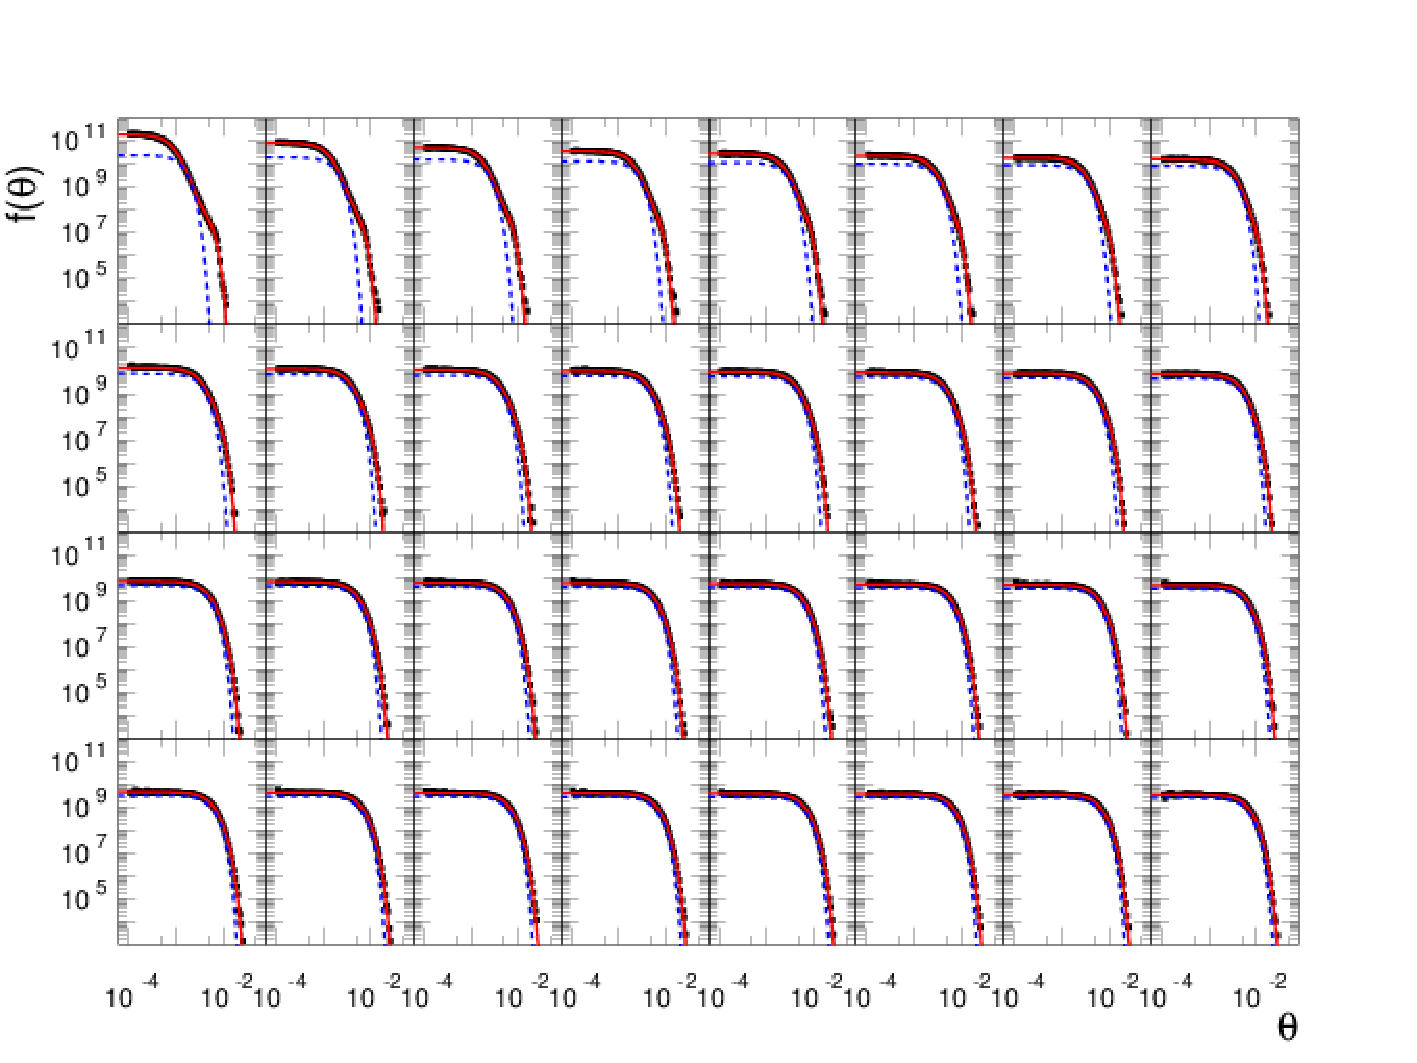
\includegraphics[width=.99\linewidth]{images/thin_theta}
    }
    \caption{Гистограммы функции плотности вероятности углового распределения многократного рассеяния $f(\theta_i)=\frac{dN_i}{\theta_i^2d\ln{\theta_i}}$ по слоям  тонкой мишени (100 бинов), $\theta_{min}=10^{-4}$ рад, $\theta_{max}=0.05$ рад, толщина слоя $ag=0.1$ мкм. Синяя штриховая кривая -- центральный гауссиан.}
    \label{fig:Thin_theta}
  \end{figure}

  Главной целью моделирования было увидеть на первых слоях (малых пробегах частиц в веществе) ``носы'' и ``хвосты'' функции плотности вероятности углового распределения многократного рассеяния (отклонения от единой функции распределения Гаусса).
  Синей штриховой кривой на Рис. ~\ref{fig:Thin_theta} показано гауссово распределение, которое при увеличении толщины станет доминировать и будет рассматриваться многими кодами как единственное распределение, описывающее многократное рассеяние.
  Видно, что для самого тонкого слоя (верхняя левая гистограмма) над постоянно растущим с толщиной основным гауссовым распределением возвышается более узкий ``нос'', который при нулевых углах отклонения превосходит основное распределение почти на порядок.
  Однако видно, что уже к восьмому слою вклад `носа'' в нулевые углы отклонения сравнивается с основным гауссом, а затем постепенно и вовсе исчезает.
  В гистограмме самого тонкого слоя (верхняя левая гистограмма) видно также, что события ``хвоста'' тянутся по крайней мере вдвое дальше, чем для основного распределения.
  Более точная аппроксимация покажет, что полная ``гауссизация'' углов отклонения частиц от их первоначального направления в результате многократного рассеяния в смысле исчезновения ``носа'' ещё не произошла даже после прохождения потоком дейтронов 32 слоёв, т. е. 3.2 мкм в материале мишени, а до области исчезновения ``хвоста'' мы ещё по толщине слоя не дошли даже в толстой мишени.

  Чтобы дальше проследить процесс ``гауссизации'', в толстой мишени величина $ag$ была увеличена в 32 раза так, чтобы теперь один слой равнялся по толщине  всем 32 слоям тонкой мишени, и моделирование было проведено при этой новой толщине слоя $ag=3.2$ мкм (общая толщина мишени около 0.1 мм).
  При этом максимальная верхняя граница гистограммы по $\theta$ была увеличена в 5 раз: $\theta_{max}=0.25$ радиан.
  Для того чтобы можно было сравнивать новые гистограммы со старыми (соответствующими толщине слоя $ag=0.1$ мкм), было необходимо сделать так, чтобы шкалы по $\theta$ совпадали.
  Если раньше было $\ln{\theta_{max}}-\ln{\theta_{min}}=\ln{\left( 5\cdot10^{-2} \right)}-\ln{10^{-4}}=\ln{500}$, то теперь стало $\ln{\theta_{max}}-\ln{\theta_{min}}=\ln{\left( 25\cdot10^{-2} \right)}-\ln{10^{-4}}=\ln{2500}$.
  Интегралы от полученных $\frac{dN_i}{d\ln{\theta_i}}$ распределений равны $\frac{10^6}{\Delta ln(\theta)}$, поэтому для сравнения распределений для тонкой и толстой мишени необходимо было умножить новые (при $ag=3.2$ мкм) значения $\frac{dN_i}{d\ln{\theta_i}}$ на коэффициент $k=\frac{\ln{500}}{\ln{2500}}=0.7943$.
  Распределения и их аппроксимация для толстых слоёв представлены на Рис. ~\ref{fig:Thick_theta}.

  \begin{figure}[ht]
    {
       \includegraphics[width=.99\linewidth]{images/thick_theta}
    }
    \caption{Гистограммы функции плотности вероятности углового распределения многократного рассеяния $f(\theta_i)=\frac{dN_i}{\theta_i^2d\ln{\theta_i}}$ для толстой мишени. Получены при 100 бинах, $\theta_{min}=10^{-4}$ рад, $\theta_{max}=0.25$ рад, 32 слоях и толщине слоя $ag=3.2$ мкм. Синяя штриховая кривая -- центральный гауссиан.}
    \label{fig:Thick_theta}
  \end{figure}

  Отличие синей пунктирной от сплошной красной кривой заметно только на первых толщинах, однако это следствие очень грубого масштаба, который необходим для анализа всех точек гистограммы, а более точно это можно проследить по параметризации зависимости ширины и амплитуды трёх гауссов от толщины слоя.
  Если считать, что ``носов'' и ``хвостов'' распределений уже нет, то есть произошла полная ``гауссизация'', то угловое распределение многократного рассеяния будет описываться основной гауссовой функцией $\frac{dN_2}{d\theta}=\frac{W_2}{D_2}\theta e^{-\frac{\theta^2}{2D_2}}$, где $W_2$ -- это интеграл основного распределения, которое должно доминировать при больших толщинах, а $D_2$ -- это дисперсия основного распределения ($D=\sigma^2$).
  Аналогично опишем ``нос'' распределения гауссианом $\frac{dN_1}{d\theta}=\frac{W_1}{D_1}\theta e^{-\frac{\theta^2}{2D_1}}$ ($D_1 < D_2$), и ``хвост'' распределения гауссианом $\frac{dN_3}{d\theta}=\frac{W_3}{D_3}\theta e^{-\frac{\theta^2}{2D_3}}$ ($D_3 > D_2$).
  Множитель $\theta$ входит в элемент угловой площади, который равен $2\pi \theta d\theta$.
  Суммируя все три распределения нужно получить одинаковую величину (миллион событий, делённый на $\Delta ln(\theta)$): $\sum_{i=1}^{3}\int \limits_0^{\infty} \frac{W_i}{D_i}e^{-\frac{\theta^2}{2D_i}}\theta d\theta=\sum_{i=1}^{3}W_i=\frac{N_p}{\Delta ln(\theta)}$, где $N_p=10^6$ -- суммарное число событий во всех бинах (полное число запущенных частиц).

Аппроксимация функции плотности вероятности углового распределения многократного рассеяния дейтронов на ионах кристаллической решётки $TiD_2$ проводилась на основе следующей функции, описывающей центральное распределение Гаусса с добавленными гауссовыми членами ``носа'' и ``хвоста'':
\begin{equation}
\label{MSApproximationFunction}
\begin{aligned} 
f(\theta)=\sum_{i=1}^{3} \frac{W_i}{D_i}e^{-\frac{\theta^2}{2D_i}}.
\end{aligned}
\end{equation}
  Первый член суммы описывает ``нос'' распределения, второй -- основной гауссиан, а третий --  ``хвост'' распределения.
  Интегрировать надо не плотность вероятности, а функцию $\theta\cdot f(\theta)$, поскольку число событий в бине пропорционально и угловой площади, пропорциональной углу $\theta$.
  Тогда неопределённый интеграл будет равен $W\cdot e^{-\frac{\theta^2}{2D}}$.
  Розыгрыш угла начинается с того, что выбирается одно из гауссовых распределений, относительные вероятности которых рассчитываются по формуле $\frac{W_i}{\sum_{i=1}^{3}W_i}$.
  Угол для выбранного Гауссова распределения разыгрывается как $\theta=\sqrt{-2D\cdot\ln{R}}$, где $R$ -- случайное число от 0 до 1, то есть используется функция, обратная к гауссовой экспоненте.
  Все шесть параметров $W_i$, $D_i$ зависят только от толщины пройденного слоя $x$, измеряемой в мкм.
  Аппроксимировались 64 распределения, построенные на Рис. ~\ref{fig:Thin_theta}, ~\ref{fig:Thick_theta} (чёрными точками для каждого слоя тонкой и толстой мишеней).

  \begin{figure}[ht]
    {
       \includegraphics[width=0.99\linewidth]{images/pars135}
    }
    \caption{Изменение интегралов трёх гауссовых кривых с увеличением толщины слоя.}
    \label{fig:Par1theta}
  \end{figure}

  Результат аппроксимации интегральных величин $W_i$ показан на Рис. ~\ref{fig:Par1theta}.
  Интеграл ``носа'' описывается формулой:
\begin{equation}
\label{MSApproximationW1}
\begin{aligned} 
W_1(x)= \frac{33390\cdot (1+\left(\frac{x}{17.1}\right)^{0.88})}{x^{0.12} \cdot \left(1+\left(\frac{x}{0.636}\right)^{1.16}\right) \cdot \left(1+\left(\frac{x}{6.128}\right)^{2.05}\right)},
\end{aligned}
\end{equation}
  которая показана на Рис. ~\ref{fig:Par1theta} чёрной кривой, проведенной через параметры, найденные при аппроксимировании 64 распределений, показанных на Рис. ~\ref{fig:Thin_theta}, ~\ref{fig:Thick_theta}.
  Члены в знаменателе описывают ускоряющееся падение параметра, а скобка в числителе несколько замедляет падение, хотя при большей статистике может оказаться, что такое замедление не нужно.
  Видно, что на самых первых тонких толщинах вклад носа доминирует, вдвое превосходя вклад основного гауссиана (красная кривая), а в последнем слое тонкой мишени становится уже на порядок меньше вклада основного гауссиана.
  На толстой мишени он падает ещё на два порядка, и надёжно выделить его при имеющихся статистических погрешностях становится невозможно.
  Заметим, что большие толщины требуют большего времени моделирования, поэтому повышать статистику ради исчезающего вклада нет смысла.
  Понятно, что на исследованных толщинах мишени вклад ``носа'' можно считать полностью исчезнувшим, поэтому в реальных экспериментах об этом вкладе даже не упоминают, хотя для моделирования радиационной стойкости этот вклад может быть самым важным.

Интеграл основного гауссиана описывается формулой:
\begin{equation}
\label{MSApproximationW2}
\begin{aligned} 
W_2(x)= \frac{22979\cdot \left(1+\frac{0.0717}{x}\right)\cdot \left(1+\left(\frac{x}{9.628}\right)^{0.032}\right)}{1+\frac{0.27}{x}}.
\end{aligned}
\end{equation}
  Зависимость от пройденной толщины основного гауссиана показана на Рис. ~\ref{fig:Par1theta} красной кривой.
  Красная кривая при стремлении толщины к бесконечности должна приблизиться к чёрной пунктирной кривой, которая определяется статистикой.
  При стремлении толщины к бесконечности вклад ``хвоста'' должен постепенно исчезнуть, как это произошло и с вкладом ``носа'', однако при малых толщинах в реальных экспериментах вклад ``хвоста'' может и сохраниться.
  Можно отметить, что в исследованном диапазоне вклад основного гауссиана возрастает примерно в 2.5 раза, а при меньших толщинах он имеет тенденцию к снижению.
  Заметим ещё, что наш результат получен для случая, когда большие переданные импульсы в Резерфордовском рассеянии обрезаны и перенесены в дискретное моделирование.
  Если пытаться учесть полное Резерфордовское рассеяние, вклад ``хвоста'' будет значительно больше, и он будет падать значительно медленнее, чем гауссово распределение.
  По этой причине в реальных экспериментах обнаруживаются широкие ``крылья'', которые в нашем случае будут определяться дискретным рассеянием, учитывающим интерференцию резерфордовского и сильного рассеяния.

Интеграл ``хвоста'' описывается формулой:
\begin{equation}
\label{MSApproximationW3}
\begin{aligned} 
W_3(x)= \frac{21859}{x^{0.09}\cdot\left(1+\left(\frac{0.8884}{x}\right)^{1.08}\right)},
\end{aligned}
\end{equation}
  которая показана на Рис. ~\ref{fig:Par1theta} синей кривой.
  Из формулы (\ref{MSApproximationW3}) видно, что вклад ``хвоста'' при больших толщинах падает обратно пропорционально $x^{0.09}$.
  Однако в исследуемом диапазоне падение не так заметно, поскольку при уменьшении толщины вклад ``хвоста'' также падает, то есть мы исследовали область, где вклад ``хвоста'' достигает максимума.
  
  \begin{figure}[ht]
    {
       \includegraphics[width=0.99\linewidth]{images/check_norm_constant}
    }
    \caption{Оценка статистической и систематической точности аппроксимации.}
    \label{fig:Norma}
  \end{figure}
  
  Точность аппроксимации можно проверить, сравнив величину интеграла $\int_0^\infty\theta\cdot f(\theta)d\theta$, где $f(\theta)$ определена формулой (\ref{MSApproximationFunction}) с величиной количества разыгранных событий $10^6$, которой интеграл должен быть равен.
  На Рис. ~\ref{fig:Norma} показано отношение интеграла к $10^6$, которое должно быть равно единице для всех исследованных толщин (напомним, что большие толщины приведены к бину по $\ln(\theta)$ величиной $k=\frac{\ln{500}}{\ln{2500}}=0.7943$).
  Из рисунка видно, что максимальные отклонения -- порядка промилле ($10^{-3}$), что и соответствует набранной статистике ($\frac{1}{\sqrt{10^6}}$).
  Тем не менее, надо отметить, что разбиение на равные логарифмические бины при росте ширины по $\theta$ приводит к систематическим отклонениям: сначала падению нормировки из-за увеличения числа частиц в младших бинах, где распределение растёт, а затем росту за счёт увеличения частиц в старших бинах, где распределение падает.
  По причине этих систематических отклонений не имело смысла увеличивать статистическую точность.
  Если пытаться увеличить точность, то вместе с увеличением числа разыгрываемых частиц надо увеличивать число бинов по $\ln{\theta}$.
  
  \begin{figure}[ht]
    {
       \includegraphics[width=0.99\linewidth]{images/pars246}
    }
    \caption{Изменение дисперсий трёх гауссовых кривых с увеличением толщины слоя.}
    \label{fig:DispTheta}
  \end{figure}
  
  На Рис. ~\ref{fig:DispTheta} показан рост удвоенной дисперсии гауссианов при увеличении толщины пройденного слоя.
  Изменение дисперсии основного гауссиана показано красной кривой.
  Цвета кривых соответствуют цветам на Рис. ~\ref{fig:Par1theta}.
  Приблизительно на тот же наклон, но несколько позже выходит и зависимость от толщины ``хвоста'', ширина которого остаётся всегда больше, чем ширина основного распределения.
  А вот ширина ``носа'', хоть и остаётся всегда меньшей ширины основного гауссиана, но сначала приближается к нему по ширине, а по мере исчезновения ширина ``носа'' сужается.
  Дисперсия ``носа'' является самой маленькой и описывается формулой:
\begin{equation}
\label{MSApproximationD1}
\begin{aligned} 
D_1(x)=\frac{0.59\cdot 10^{-5}\cdot x}{1+\frac{0.029}{x}} 
\end{aligned}
\end{equation}
С увеличением толщины дисперсия растёт приблизительно пропорционально толщине, то есть в дважды-логарифмическом масштабе стремится к прямой.
Это видно и из рисунка, и из формулы, в которой знаменатель с ростом $x$ обращается в единицу.
Для того, чтобы сохранялась монотонность гауссиан и при изменении толщины не происходило переключения с одного гауссиана на другой, приближались не сами дисперсии, а изменение дисперсии от предыдущего гауссиана.
Таким образом, рост дисперсии основного распределения описывается формулой:
\begin{equation}
\label{MSApproximationD2}
\begin{aligned} 
D_2(x)=D_1(x)+0.854\cdot 10^{-6}\cdot\left( 1+(\frac{x}{0.25})^{1.108}\right). 
\end{aligned}
\end{equation}
С увеличением $x$ различие между дисперсией гауссиана ``носа'' и дисперсией основного гауссиана увеличивается, что и видно на рисунке как отличие между красной и чёрной кривыми.
Однако это отличие само растёт почти линейно, поэтому отклонение от линейного закона невелико.
Соответственно, рост дисперсии ``хвоста'' описывается как
\begin{equation}
\label{MSApproximationD3}
\begin{aligned} 
D_3(x)=D_2(x)+0.8\cdot 10^{-5}\left( 1+(\frac{x}{1.28})^{0.77}\right)\cdot\left( 1+(\frac{x}{132.37})^{4.64}\right), 
\end{aligned}
\end{equation}


  \begin{figure}[ht]
    {
       \includegraphics[width=0.99\linewidth]{images/rms}
    }
    \caption{Сравнение полной дисперсии распределения по углу рассеяния численного эксперимента с ожидаемой зависимостью для полного Резерфордовского рассеяния при больших толщинах, когда произошла полная гауссизация углового распределения.}
    \label{fig:Check246}
  \end{figure}
  Полную дисперсию распределения (среднеквадратичное отклонение от нуля) можно посчитать, сложив дисперсии всех трёх гауссианов с весами их интегралов: $D=\frac{D_1\cdot W_1+D_2\cdot W_2+D_3\cdot W_3}{W_1+W_2+W_3}$.
  На Рис. ~\ref{fig:Check246} полная дисперсия численного эксперимента показана красной прямой.
  Эту зависимость надо сравнить с тем, что обычно используют для многократного рассеяния (формула (\ref{T0MultHE})).  
  Для рассеяния дейтрона ($z=1$) на дейтериде титана формула (\ref{T0MultHE}) принимает вид ($c=1$, а значит $\beta_{LS}=\frac{p_{LS}}{E_{LS}}$):
\begin{equation}
  \label{CheckTheta0Coefficient}
  \theta_0=\frac{13.6 \cdot \sqrt{\frac{x\cdot \rho}{X_0}}}{\beta_{LS}\cdot p_{LS}}\cdot\left[ 1+0.038\cdot\ln\left(\frac{x\cdot \rho}{X_0\cdot \beta^2_{LS}}\right)\right],
\end{equation}
где $x$ измеряется в сантиметрах, $X_0$ измеряется в г/см$^2$, поэтому используется плотность $\rho_{TiD_2}=3.91$~г/см$^3$, а $E_{LS}$ и $p_{LS}$ -- энергия и импульс налетающего дейтрона в лабораторной системе, измеряемые в МэВ. Для налетающего дейтрона с массой покоя $m_D=1875.6$ МэВ и кинетической энергией $T_{LS}=10$ МэВ его импульс $p_{LS}=193.94$ МэВ и полная энергия $E_{LS}=1885.6$ МэВ. Радиационная длина $TiD_2$ вычисляется из соотношения:
\begin{equation}
  \label{RadLength}
  \frac{A_{TiD_2}}{X_{0_{TiD_2}}}=\frac{2 A_{D}}{X_{0_{D}}}+\frac{A_{Ti}}{X_{0_{Ti}}},
\end{equation}
где $A_i$ -- масса молекулы/элемента молекулы в атомных единицах массы (а.е.м.), а $X_{0_i}$ -- радиационная длина.
  Так как $A_{TiD_2}=51.89$, $A_{D}=2.01$ и $A_{Ti}=47.87$, а также $X_{0_{D}}=125.98$ г/см$^2$ и $X_{0_{Ti}}=16.16$ г/см$^2$ \cite{PDG}, то $X_{0_{TiD_2}}=17.33$ г/см$^2$.

  На Рис. ~\ref{fig:DispTheta} полученная нами зависимость полной дисперсии распределения сравнивается с дисперсией, вычисленной по формуле (\ref{CheckTheta0Coefficient}). Это формула эмпирическая, полученная для полного Резерфордовского рассеяния, а не только для той части, которая соответствует рассеянию на ядре мишени без его выбивания из кристаллической решётки.
  Всё Резерфордовское рассеяние, включая широкое ``крыло'' рассеяния на большие углы, для которого надо учитывать интерференцию с сильной амплитудой рассеяния, приводит к распределению, которое в основном (около 98\%) приблизительно описывается гауссианом, для которого и рассчитывается дисперсия, а остальные 2\% расположены в широких ``крыльях'', обусловленных, как Резерфордовским рассеянием на большие углы, так и ядерным упругим рассеянием, а точнее их сложной интерференцией.
  Эмпирическая формула (\ref{CheckTheta0Coefficient}) была получена для релятивистских частиц и для относительно больших толщин.
  Тем не менее из рисунка видно, что её экстраполяция в область нерелятивистских частиц ($\beta\approx 0.1$) и тонких слоёв даёт неплохое предсказание.
  Но надо отметить, что, поскольку она получена для полного Резерфордовского рассеяния, она должна быть везде больше, чем результат численного эксперимента, в то время как на толщинах  меньше одного микрона она идёт ниже, то есть этой аппроксимацией уже пользоваться нельзя.
  То, что полученное значение меньше теоретического, обусловлено тем, что при выводе формулы (\ref{T0MultHE}) рассматривался диапазон значений $|t|$ от 0 до $|t|_{max}$, а моделирование проводилось при $|t|$ от 0 до $|t|_{min} \ll |t|_{max}$.
  Кроме того, используя эту аппроксимацию, не вполне понятно, что делать с теми 2\% частиц,  рассеянных на большие углы.
  Попытка придумать аппроксимацию для ``крыльев'' не имела успеха.
  Обычно считают, что эти крылья можно описывать ядерным упругим рассеянием, но на поверку оказывается, что при низких энергиях это рассеяние за вычетом Резерфордовского рассеяния оказывается отрицательным.
  В нашем алгоритме таких проблем нет.
  Всё, что мы не учли в многократном рассеянии (события с выбиванием атома из кристаллической решётки), моделируется как независимые дискретные процессы, примеры которых будут представлены в следующих разделах.
  При моделировании ионного каскада к двум процессам, -- пробегу до пересечения с границами вокселя без взаимодействий и многократному рассеянию, -- добавится третий -- дискретное упругое рассеяние на углы, большие, чем максимальный угол многократного рассеяния, определяемый по формуле (\ref{Xp}) как $2\arcsin{\sqrt{ \frac{|t|_{min}}{4 p_{CM}^2}} }$.
  Для описания дифференциального сечения упругого дейтрон-дейтронного рассеяния используется аппроксимация, полученная в разделе \ref{subPol1}.
  Из-за большого кулоновского барьера упругое рассеяние дейтрона на ядре титане и ядер титана друг на друге описывается только дифференциальным сечением Резерфордовского рассеяния.
 
\subsection{ТРТ аппроксимация дифференциальных сечений упругого $pp$ рассеяния}
\label{subPol0}

  В процессе выполнения работы была накоплена обширная база данных для рассеяния лёгких ионов на различных ядрах.
  Поскольку для создания нового дискретного процесса многократного рассеяния в тонких слоях программный комплекс ТРТ использует универсальные решения, необходимо было сосредоточиться на ядерном дифференциальном угловом сечении, которое при интегрировании даёт полное ядерное упругое сечение.
  В первую очередь необходимо было получить результаты для рассеяния ионов водорода (протонов) и гелия ($\alpha$-частиц).
  На сегодняшний день теоретически решение этого вопроса неоднозначно.
  Для описания дифференциальных угловых распределений традиционно используют оптические модели \cite{Sys_pA}, зависящие от большого числа параметров, как самого оптического потенциала, так и радиального распределения плотности ядра.
  Существуют и другие модели расчёта дифференциальных угловых распределений, но большинство из них всё равно сводится к параметризации сечений.
  В этом смысле простая и удобная для моделирования параметризация самих дифференциальных сечений ничем не хуже модельной со сравнимым числом свободных параметров.
  Главным вопросом остаётся предсказательная сила такой параметризации, поскольку данные имеются для ограниченных энергетических диапазонов и небольшого набора ион-ионных пар.
  Возникает вопрос: насколько надёжной можно считать экстраполяцию или интерполяцию зависимости параметров, описывающих упругое сечение в области энергий для ион-ионных пар, для которых нет экспериментальных данных?
  Ответ на этот вопрос можно получить, оценивая качество аппроксимации дифференциальных сечений при непрерывной параметризации параметров дифференциального сечения как функций начальной энергии и атомного веса ядра-мишени.

  При упругом рассеянии лёгких ионов (с атомным весом $a$) большой вклад даёт $t$-канальное рассеяние, примером которого является кулоновское рассеяние с $t$-канальным обменом виртуальным $\gamma$-квантом или $\pi^0$-мезоном, и $u$-канальное рассеяние, когда налетающая частица подхватывает $A-a$ нуклонов ядра мишени и сама превращается в ядро-мишень с числом нуклонов (атомным весом) $A$.
  Очевидно, что в системе центра масс при $u$-канальном обмене протон как бы рассеивается назад, причём при приближении угла рассеяния к 180$^o$ сечение не убывает, а растёт.
  Этот эффект называется ядерной глорией \cite{NuclGlor} и при низких энергиях имеет достаточно большую вероятность.
  Понятно, что никакие оптические потенциалы не могут с достаточной точностью рассчитывать этот эффект, а при свободной форме, описывающей дифференциальное сечение упругого рассеяния, этот эффект учесть можно.

  При описании кулоновского барьера упругого рассеяния используется величина, называемая энергией Гамова, которая определяется как \cite{Gamow1928,ThermonuclearReactionRates_GamowEnergy}:
\begin{equation}
  \label{GamovEnergyp}
  E_{g}=2 \mu \cdot \left( \pi \cdot \alpha \cdot z \cdot Z \right)^2.
\end{equation}
В случае рассеяния протона на протоне приведённая масса рассчитывается как $\mu=\frac{m \cdot M}{m+M}=\frac{m_p}{2}$, где $m_p=938.3$ МэВ -- масса покоя протона, а когда частицы разные, $m$, $M$ и $z$, $Z$ -- массы и заряды налетающей частицы и мишени соответственно. Для реакции упругого $pp$ рассеяния (когда $m=M=m_p$ и $z=Z=1$) $E_g=0.493$ МэВ.

Энергия Гамова используется в так называемом факторе Гамова \cite{ThermonuclearReactionRates_GamowEnergy}, описывающем вероятность того, что рассеивающиеся частицы преодолеют кулоновский барьер, которая записывается в виде:
\begin{equation}
  \label{GamovPp}
  P=\exp{ \left( -\sqrt{\frac{E_g}{T_{CM}}} \right)  }, 
\end{equation}
где $T_{CM}$ - полная кинетическая энергия в системе центра масс ($T_{LS}$ -- в лабораторной системе), равная в случае рассеяния одинаковых частиц половине энергии налетающей частицы:
\begin{equation}
  \label{GamovFactorp}
  T_{CM}=\frac{T_{LS}}{2}. 
\end{equation}
Для того, чтобы рассчитать полную амплитуду рассеяния, необходимо знать выражение Резерфордовской амплитуды рассеяния протона на протоне. Амплитуда Резерфордовского рассеяния различных частиц определяется как
\begin{equation}
  \label{ARp}
A_R=2\mu \alpha z Z \cdot \sqrt{\frac{\pi}{p_{CM}^2}},
\end{equation}
где 
\begin{equation}
  \label{Pcmp}
  p_{CM}=\frac{p_{LS} \cdot M}{\sqrt{s}}
\end{equation}
-- импульс в системе центра масс реакции, а  $p_{LS}$ -- импульс налетающей частицы в лабораторной системе, $\mu=\frac{m_p}{2}$ -- приведённая масса реакции.
  Мандельстамовская переменная $s$ определена в виде:
\begin{equation}
  \label{MandelstamSp}
s=m^2+2E_{LS}\cdot M+M^2.
\end{equation}
  В нерелятивистском пределе: $s\approx\left( m+M \right)^2$, $E_{LS}=m_p+T_{LS}$ -- полная энергия налетающего протона в лабораторной системе (мишень покоится).
  Для $pp$ рассеяния выражение $s$ через кинетическую энергию можно упростить:
\begin{equation}
  \label{MandelstamSTcmp}
s=4m_p^2 \cdot \left( 1+ \frac{T_{LS}}{2m_p} \right) =4m_p^2 \cdot \left( 1+ \frac{T_{CM}}{m_p} \right).
\end{equation}

  В формуле (\ref{ARp}) $\frac{\pi}{p_{CM}^2}$ -- это якобиан перехода от $\frac{d\sigma}{d\Omega_{CM}}$ к $\frac{d\sigma}{d|t|}$:
\begin{multline}
  \label{Jacobianp}
\frac{d\sigma}{d|t|}=\frac{d\sigma}{d(2p_{CM}^2 \cdot (1-\cos{\theta_{CM}}))}=-\frac{d\sigma}{2p_{CM}^2 \cdot d(\cos{\theta_{CM}})}= \\ =\frac{1}{2p_{CM}^2} \cdot \int_0^{2\pi} \frac{d\sigma}{d\Omega_{CM}} d\phi=\frac{\pi}{p_{CM}^2} \cdot \frac{d\sigma}{d\Omega_{CM}}.
\end{multline}
Здесь $\theta_{CM}$ -- угол рассеяния в системе центра масс, элемент телесного угла $d\Omega_{CM}=d\phi \cdot d(1-\cos{\theta_{CM}})$, $\phi$ -- азимутальный угол, а мандельстамовская переменная $|t|$ (равная квадрату переданного во взаимодействии поперечного импульса) определяется как
\begin{equation}
 \label{Xp} 
|t|=2p_{CM}^2 \cdot (1-\cos\theta_{CM})=4p_{CM}^2 \sin^2\frac{\theta_{CM}}{2}=2T_{recoil}M.
\end{equation}
Последнее равенство в (\ref{Xp}), где $T_{recoil}$ -- кинетическая энергия ядра отдачи, получается, если записать переменную $|t|$ для ядра мишени, а не для налетающей частицы, как в первых двух равенствах.

Дифференциальное сечение Резерфордовского рассеяния полностью ионизированных ядер определяется выражением \cite{LandauLifshitzMechanics}
\begin{equation}
  \label{dSigmadModtp}
  \frac{d\sigma}{d\Omega_{CM}}=\left( \frac{2 \mu \alpha z Z}{t} \right)^2 \cdot \left( \hbar c \right)^2.
\end{equation}
Объединение формул (\ref{Jacobianp}) и (\ref{dSigmadModtp}) даёт
\begin{equation}
  \label{Dimension1p}
  \frac{d\sigma}{d|t|}=\left( \frac{A_R}{t} \right)^2 \cdot \left( \hbar c\right)^2,
\end{equation}
где $\hbar c\approx 200$ МэВ$\cdot$ фм -- коэффициент перевода МэВ$^{-1}$ в фм.
  При теоретических расчётах использовалась система единиц $\hbar=1$ и $c=1$, а потом при пересчёте к необходимым единицам добавлялся коэффициент $\hbar c$.

  При низких энергиях ядра экранированы электронами, поэтому на больших расстояниях, соответствующих по соотношению неопределённости малым квадратам переданного импульса, рост $\frac{1}{t^2}$ при стремлении $|t|$ к нулю обрезается параметром электронной экранировки $A_s$, использованным  в формуле (\ref{MS1}).
  Обычно вводят параметр электронной экранировки в виде $\mu^2_S=4p^2_{CM}\cdot A_S$, тогда он оказывается независимым от энергии налетающей частицы и Резерфордовское сечение оказывается пропорциональным фактору $\frac{1}{(|t|+\mu^2_S)^2}$, то есть принимает вид полюсного $t$-канального члена, который возникает, например, при обмене $\pi^0$ мезоном: $\frac{1}{(t-m_{\pi^0}^2)^2}$ (напомним, что $t$ -- величина отрицательная: $t=-|t|$).
 Однако величина константы электронной экранировки лежит много ниже величины $|t|_{min}$, выше которой работает дискретный процесс ($\mu^2_S \ll |t|_{min}$), поэтому при расчёте многократного рассеяния мы эту величину учитывали, а при моделировании дискретного процесса мы этой малой величиной пренебрегаем.

Резерфордовское дифференциальное сечение протон-протонного рассеяния с учётом тождественности частиц и того, что спин протона равен $\frac{1}{2}$, записывается в виде ($\hbar c=1$)  \cite{LandauLifshitzNonrelativisticQM}:
\begin{equation}
  \label{dSigmadOmegaCMpFull}
  \frac{d\sigma_R}{d\Omega_{CM}}=\left( \frac{zZ \alpha\mu^2}{m_p p_{CM}^2} \right)^2\left( \frac{1}{\sin^4{\frac{\theta_{CM}}{2}}} + \frac{1}{\cos^4{\frac{\theta_{CM}}{2}}} - \frac{\cos{\left( \frac{\alpha\ln{ \left( \tg^2{\frac{\theta_{CM}}{2}} \right)}}{\beta_{CM}}\right)}}{\sin^2{\frac{\theta_{CM}}{2}}\cos^2{\frac{\theta_{CM}}{2}}}\right),
\end{equation}
где $\beta_{CM}=\frac{p_{CM}}{E_{CM}}$ -- скорость приведённой частицы в системе центра масс, а $P$ определяется формулой (\ref{GamovPp}).
  Если бы был учтён параметр экранировки, то все $\sin^2{\frac{\theta_{CM}}{2}}$, пропорциональные $|t|$ надо было бы заменить на $\sin^2{\frac{\theta_{CM}}{2}}+\frac{\mu^2_S}{4p^2_{CM}}$ и все $\cos^2{\frac{\theta_{CM}}{2}}$, пропорциональные $|u|$ надо было бы заменить на $\cos^2{\frac{\theta_{CM}}{2}}+\frac{\mu^2_S}{4p^2_{CM}}$, что мы и сделаем, когда при описании $d-d$ упругого рассеяния будем рассматривать $t/u$-канальные амплитуды.
  Для $p-p$ рассеяния $t/u$-канальные амплитуды много меньше $s$-канальной амплитуды, поэтому мы будем ими пренебрегать, хотя при очень больших энергиях, когда будут достигаться $|t|\gg m^2_{\pi^0}$, $t/u$-амплитуды и могут оказаться необходимыми.
  Мы сознательно не рассматривали этот диапазон, поскольку для него существует устоявшаяся теория \cite{Norman09}, использующая модель одно-бозонного обмена (OBEM -- One-Boson Exchange Model) \cite{OBEM}, которая является обобщением хорошо известной модели одно-пионного обмена (OPEM -- One-Pion Exchange Model).

В приближении $\alpha \ll \beta$ (высокие энергии) косинус в последнем слагаемом правой части выражения (\ref{dSigmadOmegaCMpFull}) обращается в единицу, и при учёте того, что для $pp$ рассеяния $z=Z=1$, оно принимает вид:
\begin{equation}
  \label{dSigmadOmegaCMp}
\frac{d\sigma_R}{d\Omega_{CM}}=\left( \frac{\alpha\mu^2}{m_p p_{CM}^2} \right)^2 \left( \frac{1}{\sin^4{\frac{\theta_{CM}}{2}}} + \frac{1}{\cos^4{\frac{\theta_{CM}}{2}}} - \frac{1}{\sin^2{\frac{\theta_{CM}}{2}}\cos^2{\frac{\theta_{CM}}{2}}} \right).
\end{equation}

После несложных преобразований для высоких энергий из (\ref{dSigmadOmegaCMp}) получаем:
\begin{equation}
  \label{dSigmadOmegaSimplep}
\frac{d\sigma_R}{d\Omega_{CM}}=\left( \frac{4 \alpha \cdot \mu^2}{m_p \cdot p_{CM}^2} \right)^2 \cdot \frac{1-\frac{3}{4} \sin^2{\theta_{CM}}}{\sin^4{\theta_{CM}}}.
\end{equation}

Так как в случае $pp$ рассеяния $\mu=\frac{m_p}{2}$, получаем:
\begin{equation}
  \label{EqualCoeffficientsp}
\frac{\alpha\mu^2}{m_p p_{CM}^2}=\frac{2 \mu \alpha }{4p_{CM}^2},
\end{equation}
а значит формулу (\ref{dSigmadOmegaSimplep}) можно записать в виде:
\begin{equation}
  \label{dSigmadOmegaSimple1p}
\frac{d\sigma_R}{d\Omega_{CM}}=\left( \frac{2 \mu \alpha}{t}\right)^2 \cdot \frac{1-\frac{3}{4} \sin^2{\theta_{CM}}}{\cos^4{\frac{\theta_{CM}}{2}}} \cdot \left( \hbar c \right)^2,
\end{equation}
и (\ref{dSigmadOmegaCMp}) примет вид:
\begin{equation}
  \label{dSigmadOmegaCM1p}
  \frac{d\sigma_R}{d\Omega_{CM}}=\left( \frac{2 \mu \alpha}{t} \right)^2 \cdot \left( 1 + \tg^4{\frac{\theta_{CM}}{2}} -\tg^2{\frac{\theta_{CM}}{2}} \right).
\end{equation}
Эту формулу можно использовать для ускорения вычислений, поскольку отличие от единицы величины косинуса $\cos{\left( \frac{\alpha\ln{ \left( \tg^2{\frac{\theta_{CM}}{2}} \right)}}{\beta_{CM}}\right)}$ в формуле (\ref{dSigmadOmegaCMpFull}), на который надо умножить третий член в скобке, практически не сказывается на величине дифференциального сечения даже при малых энергиях.

Поскольку
\begin{equation}
  \label{dSigmadOmegaCM2p}
  \frac{d\sigma_R}{d|t|}=\frac{d\sigma_R}{d\Omega_{CM}} \cdot \frac{\pi}{p_{CM}^2},
\end{equation}
безразмерную амплитуду Резерфордовского рассеяния тождественных частиц в случае $pp$ рассеяния можно записать в виде:
\begin{equation}
  \label{Artotp}
  A_{Rtot}^{p-p}=A_R \cdot \frac{\sqrt{1-3 \sin^2{\frac{\theta_{CM}}{2}} \cdot \left( 1-\sin^2{\frac{\theta_{CM}}{2}} \right) }}{1-\sin^2{\frac{\theta_{CM}}{2}}},
\end{equation}
где $sin^2{\frac{\theta_{CM}}{2}}$ выделено для того, чтобы его можно было заменить на $|t|$ (формула (\ref{Xp}))
  Тогда Резерфордовское сечение упругого рассеяния протона на протоне упрощается:
\begin{equation}
  \label{dSigmadTp}
  \frac{d\sigma_R^{p-p}}{d|t|}=\left( \frac{A_{Rtot}^{p-p}}{t} \right)^2.
\end{equation}

Запишем действительную и мнимую части полной амплитуды $pp$ рассеяния $A$, в которой сильная и электромагнитная амплитуды интерферируют, в виде: 
\begin{equation}
  \label{Term1p}
  Re(A)=\frac{A_{Rtot}^{p-p}}{|t|}+\frac{A_s}{s} \cdot \cos(\phi_s)
\end{equation}
и
\begin{equation}
  \label{Term2p}
  Im(A)=\frac{A_s}{s} \cdot \sin(\phi_s),
\end{equation}
где в формуле (\ref{Term1p}) для $Re(A)$ первый член соответствует амплитуде Резерфордовского рассеяния, второй -- $s$-канальному рассеянию,
а единственный член в формуле (\ref{Term2p}) для $Im(A)$ соответствует только $s$-канальному рассеянию.

Тогда полученная аппроксимация запишется в виде:
\begin{equation}
 \label{Finddp}     
      \frac{d\sigma}{d|t|}=\left( \hbar c\right)^2 \cdot \left( Re^2(A)+Im^2(A) \right),
\end{equation}
  Здесь $|t|$ изменяется от 0 до величины $\frac{|t|_{max}}{2}$.
  Половина $|t|_{max}$ из-за того, что частицы тождественные, а значит, в системе центра масс $\frac{d\sigma}{d|t|}$ симметрично относительно $\frac{\pi}{2}$: $|t|=|t|_{max}\cdot \sin^2{\left(\frac{\pi}{2}/2 \right)}=\frac{|t|_{max}}{2}$.

\begin{figure}[ht]
  {
       \includegraphics[width=0.99\linewidth]{images/pp}
  }
  \caption{Аппроксимация дифференциальных сечений упругого $pp$ рассеяния \cite{PP1_Wassmer,PP2_Worthigton,PP3_Blair,PP4_Imai,PP5_Johnston,PP6_Kikuchi,PP7_Berdoz,
 PP8_Taylor,PP9_Mahjour} на основе теории прямых ядерных реакций. Красная кривая - TPT аппроксимация, зелёная -- Резерфордовское дифференциальное сечение рассеяния $pp$, определяемое формулой (\ref{dSigmadTp}).}
  \label{fig:pp}
\end{figure}

\begin{figure}[ht]
  {
       \includegraphics[width=0.99\linewidth]{images/1as_pp}
  }
  \caption{Зависимость безразмерной амплитуды $s$-канала от кинетической энергии $T_{CM}$ рассеивающихся протонов в системе центра масс, использовавшаяся при аппроксимации зависимости дифференциального сечения упругого $pp$ рассеяния от кинетической энергии налетающего протона.}
  \label{fig:1as_pp}
\end{figure}

\begin{figure}[ht]
  {
       \includegraphics[width=0.99\linewidth]{images/2phases}
  }
  \caption{Зависимость фазы $s$-канала от кинетической энергии $T_{CM}$ рассеивающихся протонов в системе центра масс, использовавшаяся при аппроксимации зависимости дифференциального сечения упругого $pp$ рассеяния от кинетической энергии налетающего протона. Пунктирная линия соответствует значению фазы $\phi=\pi$ (деструктивная интерференция).}
  \label{fig:2phases_pp}
\end{figure}

Для $pp$ рассеяния аппроксимация на основе теории прямых ядерных реакций была выполнена с использованием двух параметров -- амплитуды ($A_s$) и фазы ($\phi_s$) $s$-канала, зависимости которых от кинетической энергии $T_{CM}$ протонов показаны на Рис.~\ref{fig:1as_pp} и ~\ref{fig:2phases_pp}.

Безразмерная амплитуда $s$-канала, показанная на Рис.~\ref{fig:1as_pp}, описывается формулой:
\begin{equation} 
  \label{AmplitudeSp}
   A_s= \frac{ 40000 \cdot \left( 1 + \left(\frac{T_{CM}}{3.064}\right)^{0.45} \right) \cdot \left( 1 + \frac{T_{CM}}{157.} \right) \cdot \sqrt{P} }{1 + \left( \frac{T_{CM}}{0.582}\right)^{1.45}},
\end{equation}
где фактор Гамова $P$, учитывающий проницаемость кулоновского барьера и снижающий сильную амплитуду при уменьшении энергии, определяется формулой (\ref{GamovPp}).
  Степени кинетической энергии подобраны так, чтобы при больших энергиях амплитуда выходила на константу.
  В будущем, когда для описания дифференциальных сечений при больших начальных энергиях будет добавлен вклад $t/u$ диаграмм, поведение $s$-амплитуды может быть уточнено.

Фаза $s$-канала описана нами формулой:
\begin{equation}
  \label{Phasesp}
  \phi_s= \frac{ \pi \cdot \left( 1 + \left(\frac{T_{CM}}{0.252} \right)^{9.2} \right) \cdot \left( 1 + \frac{T_{CM}}{95.2} \right) }{ \left( 1 + \left( \frac{T_{CM}}{0.243} \right)^{9.27} \right) \cdot \left( 1 + \left(\frac{T_{CM}}{99.3}\right)^{3.8} \right) }.
\end{equation}
  Начальная кинетическая энергия $T_{CM}$ в том и другом случае измеряется в МэВ.
  При стремлении к нулю энергии фаза становится полностью деструктивной ($\phi=\pi$), а при больших энергиях -- полностью конструктивной ($\phi=0$).
  В первой точке (0.5 МэВ) отчётливо проявляется деструктивная интерференция.
  Гипотеза деструктивной интерференции при малых энергиях не оказывает большого влияния на упругие дифференциальные спектры, поскольку под действием фактора Гамова сильная амплитуда $A_s$ становится при малых энергия малой величиной.
  Тенденция в последней использованной точке (190 МэВ) к уменьшению фазы позволила нам предположить, что при больших энергиях можно ожидать стремления фазы к конструктивному значению, однако это временное решение, поскольку для столь больших значений энергии надо использовать $t/u$-амплитуды, как это сделано в следующем разделе для $dd$ реакций.
  С этим связан и небольшой подъём нашей $A_s$ амплитуды с увеличением энергии по сравнению с обнаруженным падением.

  На Рис.~\ref{fig:pp} аппроксимация, полученная по формулам (\ref{Term1p})-(\ref{Finddp}), в которой использованы параметры (\ref{AmplitudeSp}) и (\ref{Phasesp}) -- амплитуда и фаза $s$-канала (красная кривая), сравнивается с доминирующей при малых квадратах переданного импульса Резерфордовской амплитудой.
  Экспериментальные данные работ \cite{PP1_Wassmer,PP2_Worthigton,PP3_Blair,PP4_Imai,PP5_Johnston,PP6_Kikuchi,PP7_Berdoz,
 PP8_Taylor,PP9_Mahjour} в основном взяты из базы ядерных данных EXFOR.

%То, что при аппроксимации удалось использовать только $s$-канальное рассеяние, может быть вызвано тем, что $t$-канальный обмен виртуальным $\pi^0$-мезоном в случае $pp$ рассеяния может быть подавлен законом сохранения изоспина.

\begin{figure}[ht]
  {
       \includegraphics[width=0.99\linewidth]{images/pp100kev}
  }
  \caption{Деструктивный вклад ядерного рассеяния для кинетической энергии налетающего протона 100 кэВ: красная кривая -- аппроксимация дифференциального сечения упругого $pp$ рассеяния на основе теории прямых ядерных реакций, зелёная кривая -- Резерфордовское дифференциальное сечение $pp$ рассеяния, определяемое по формуле (\ref{dSigmadTp}).}
  \label{fig:pp100kev}
\end{figure}

 Для сравнения на Рис.~\ref{fig:pp100kev} представлено отличие дифференциального сечения упругого $pp$-рассеяния, рассчитанного согласно полученной аппроксимации, от стандартного Резерфордовского дифференциального сечения рассеяния тождественных частиц, определяемого по формуле (\ref{dSigmadTp}), при кинетической энергии налетающего протона 100 кэВ, примерно соответствующей максимуму сечения $dt$-реакции.
  Как видно из Рис.~\ref{fig:pp100kev}, наибольшее отличие наблюдается при угле рассеяния 90 градусов (максимальный угол рассеяния в случае тождественных частиц) и составляет около 10\%, то есть в упругом рассеянии протона на протоне при низких энергиях влияние сильного взаимодействия нуклонов, определяемого радиусом взаимодействия и длиной рассеяния, является малой поправкой.
  Однако при малых энергиях в системе центра масс, когда взаимодействуют вторичные, одновременно вылетающие в одной ядерной реакции протоны, сильное взаимодействие протонов, приводящее к их перерассеянию друг на друге в поле ядра, приводит к заметному усилению выхода близких в фазовом пространстве протонов (корреляции тождественных нуклонов или близкие корреляции, противопоставляемые дальним кинематическим корреляциям).
  Это явление известно как эффект Мигдала-Ватсона \cite{MigdalPP,WatsonPP}.
  Наша аппроксимация, впервые проведённая в области самых низких энергий важна для расчёта этого эффекта, поскольку описывает спад близких корреляций протонов, обусловленный кулоновским отталкиванием вторичных протонов.
  Этот эффект может повлиять на интерпретацию измерений, делающих оценку размера области рождения жёстких вторичных частиц в ядерной физике высоких энергий.
  
  Важно отметить, что Рис.~\ref{fig:pp} поясняет также, почему ранее эта область энергий не была систематически изучена.
  Дело в том, что изучалось только сильное взаимодействие протонов, а кулоновское считалось тривиальным фактором, который иногда даже вычитался из экспериментальных значений.
  Кроме того, общепринятым являлось мнение об изотропном сильном упругом рассеянии при столь малых энергиях.
  На рисунке это выражается в практически постоянной величине $\frac{d\sigma}{dt}$ при больших $|t|$, где сильная амплитуда доминирует.
  В нашей модели это не зависящая от $|t|$ $s$-канальная амплитуда $A_s$ (диаграмма изотропного распада компаунд-ядра), а в потенциальных моделях типа OBEM (One-Boson Exchange Model) -- это $S$-волновое рассеяние.
  Существенным эффектом является то, что вместо того, чтобы складываться с Резерфордовской амплитудой  $A_R$, сильная амплитуда $A_s$ вычитается из неё, что доказывает несостоятельность подхода, основанного на независимом моделировании многократного Резерфордовского рассеяния и независимого сильного упругого рассеяния.
  

\subsection{ТРТ аппроксимация дифференциального сечения упругого dd рассеяния}
\label{subPol1}

  Базы данных сечений упругого рассеяния были собраны не только для протонов, но и для тяжёлых ионов.
  Для упругой реакции рассеяния дейтрона на дейтроне, которая использовалась при моделировании ионных каскадов в дейтриде титана, величина энергии Гамова, определяемой выражением (\ref{GamovEnergyp}), равна $E_g=0.986$ МэВ.

\begin{figure}[ht]
   \centering
   \includegraphics[width=0.95\linewidth]{images/4parfit}
   \caption{Зависимости параметров, использованных при аппроксимации упругого дифференциального сечения $dd$ рассеяния, от кинетической энергии $T_{CM}$ рассеивающихся дейтронов в системе центра масс: (a) -- $s$-канальной амплитуды $A_s$, (b) -- амплитуды объединённого $tu$-канала $A_{tu}$, (c) и (d) -- фаз $s$- и $tu$-каналов соответственно.} 
   \label{fig:4parfit_dd}
\end{figure}

  Аппроксимация упругого $dd$ рассеяния была выполнена на основе теории прямых ядерных реакций с использованием 4 параметров -- амплитуд и фаз $s$-канала и объединённого $tu$-канала (т. к. рассеиваются тождественные частицы, вклад $t$-канала совпадает по величине с $u$-каналом), изображённых на Рис.~\ref{fig:4parfit_dd}.
  Рассмотрим зависимость этих параметров от кинетической энергии $T_{CM}$ (МэВ) рассеивающихся дейтронов в системе центра масс.
  Безразмерная амплитуда объединённого $tu$-канала параметризовалась в виде:
\begin{equation}
  \label{AmplitudeTU}
A_{tu} = \frac{1041\cdot \left( 1 + \left(\frac{T_{CM}}{0.97} \right)^{3.89} \right) \cdot \sqrt{P}}{ \left( 1 + \left(\frac{T_{CM}}{0.056} \right)^{1.29} \right) \cdot \left( 1 + \left(\frac{T_{CM}}{1.574} \right)^{2.6} \right)\left( 1+\left(\frac{T_{CM}}{16.75}\right)^{1.67}\right) },
\end{equation}
где $P$ -- вероятность того, что частицы преодолеют кулоновский барьер, которая определяется выражением (\ref{GamovPp}).
  Величиной $t/u$ амплитуды в $pp$ рассеянии мы пренебрегали, поскольку для обмена пионом два протона должны сблизиться, чему препятствует кулоновский барьер.
  В случае рыхлого дейтрона, в котором среднее расстояние ($r$-компонента $\psi$-функции) -- более двух ферми, возникает возможность сближения нейтронов и обмена ими $\pi^0$-мезоном, тогда как протоны будут разделены достаточно большим расстоянием.
  По этой причине в $pp$-рассеянии этой амплитудой при малых энергиях мы пренебрегали, а для $dd$ она имеет значимую величину.
  Заметим также, что для $pp$ рассеяния амплитуда сильного взаимодействия, показанная на Рис.~\ref{fig:1as_pp}, монотонно падает, а в амплитудах $A_s$ и $A_{tu}$ имеется подъём.
  Этот подъём связан с наличием резонансов в компаунд $^4He^*$ системе.
  Не считая резонансов, которые имеют малый бранчинг в $dd$, и не рассматривая широкие резонансы: $E=$27.42($E_{CM}=$3.57), $\Gamma=$8.69 МэВ ($2^+, ^3P_1$); $E=$28.39($E_{CM}=$4.54), $\Gamma=$8.75 МэВ ($2^-$) и $E=$29.89($E_{CM}=$6.04), $\Gamma=$9.72 МэВ ($2^+, ^5D_2$), можно обратить внимание на три относительно узких резонанса как раз в области 4-5 МэВ в системе центра масс: $E=$28.37($E_{CM}=$4.52), $\Gamma=$3.92 МэВ ($1^-$); $E=$28.64($E_{CM}=$4.79), $\Gamma=$4.89 МэВ ($0^-$) и $E=$28.67($E_{CM}=$4.82), $\Gamma=$3.78 МэВ ($2^+, ^1D_2$).
  Именно они приводят к максимуму в сильных амплитудах.

  Амплитуда $s$-канала описывалась в виде:
\begin{equation}
  \label{AmplitudeStu}
A_s =  \frac{49000. \cdot \left( 1 + \left(\frac{T_{CM}}{1.173} \right)^{3.06} \right) \cdot \sqrt{P}}{ \left( 1 + \left( \frac{T_{CM}}{0.64}\right)^2 \right) \cdot \left( 1 + \left(\frac{T_{CM}}{5.45} \right)^2 \right) \cdot \left( 1 + \left(\frac{T_{CM}}{23.7}\right)^{1.775} \right)}.
\end{equation}
  Величина $s$ определяется формулой (\ref{MandelstamSTcmp}).
  Видно, что амплитуда $s$-канала почти на три порядка превосходит амплитуду $t/u$-канала, и с учётом того, что в сечении амплитуды возводятся в квадрат, можно говорить о пренебрежимо малом вкладе $t/u$-канала.
  Однако из энергетической зависимости фаз видно, что при малых энергиях они обе конструктивны по отношению к Резерфордовской амплитуде и между собой, поэтому можно ожидать существенного усиления как при больших, так и при относительно малых углах рассеяния даже при совсем малых энергиях.

Фаза $s$-канала параметризовалась в виде:
\begin{equation}
  \label{Phases}
\phi_{s}=\frac{\left(\frac{T_{CM}}{0.93}\right)^{2.76}}{ \left( 1 + \left( \frac{T_{CM}}{1.63}\right)^{2.8}\right)}.
\end{equation}

Фаза объединённого $tu$-канала:
\begin{equation}
  \label{Phasetu}
\phi_{tu}=\frac{\left(\frac{T_{CM}}{2.65}\right)^{3.1}}{ \left( 1 + \left(\frac{T_{CM}}{3.22}\right)^{3.245}\right)}.
\end{equation}
  То есть фазы сильного взаимодействия ведут себя по отношению к Резерфордовской амплитуде очень похожим образом, конструктивно усиливая друг друга при низких энергиях.
  Это также является фактором усиления вклада амплитуды сильного взаимодействия при низких энергиях.
  
  Рассмотрим теперь эффект тождественности для рассеяния частиц со спином 1.
  В случае упругого рассеяния дейтрона на дейтроне (спин дейтрона $S$=1) следует применять формулу Резерфорда в виде \cite{LandauLifshitzNonrelativisticQM}:
\begin{equation}
  \label{dSigmadOmegaCMFull}
  \frac{d\sigma_{R}}{d\Omega_{CM}}=\left( \frac{zZ\alpha\mu^2}{m_d p_{CM}^2} \right)^2\left( \frac{1}{\sin^4{\frac{\theta_{CM}}{2}}} +  \frac{1}{\cos^4{\frac{\theta_{CM}}{2}}} + \frac{2\cos{ \left( \frac{\alpha\ln{ \left( \tg^2{\frac{\theta_{CM}}{2}} \right) }}{\beta_{CM}} \right) }}{3\sin^2{\frac{\theta_{CM}}{2}}\cos^2{\frac{\theta_{CM}}{2}}}\right),
\end{equation}
где $\beta_{CM}=\frac{p_{CM}}{E_{CM}}$ -- скорость приведённой частицы в системе центра масс, а $m_d=1875.6$ МэВ -- масса покоя дейтрона. Коэффициент $\frac{2}{3}$ берётся из общего соотношения для тождественных частиц $\pm \frac{2}{2S+1}$ \cite{LandauLifshitzNonrelativisticQM}, где $S$ -- спин дейтрона, равный $1$ (положительный знак для целого спина и отрицательный для полуцелого, определяемых соответственно статистикой Бозе-Эйнштейна и статистикой Ферми).

В приближении большой скорости налетающей частицы $\alpha \ll \frac{p_{CM}}{E_{CM}}$, что соответствует случаю, когда сильные взаимодействия могут преодолеть кулоновский барьер, выражение (\ref{dSigmadOmegaCMFull}) принимает вид
\begin{equation}от толщины слоя
  \label{dSigmadOmegaCM}
  \frac{d\sigma_R}{d\Omega_{CM}}=\left( \frac{\alpha\mu^2}{m_d p_{CM}^2} \right)^2\left( \frac{1}{\sin^4{\frac{\theta_{CM}}{2}}} +  \frac{1}{\cos^4{\frac{\theta_{CM}}{2}}} + \frac{2}{3\sin^2{\frac{\theta_{CM}}{2}}\cos^2{\frac{\theta_{CM}}{2}}} \right),
\end{equation}
где учтено, что для $dd$ рассеяния $z=Z=1$. С учётом (\ref{EqualCoeffficientsp}) оно упрощается до вида:
\begin{equation}
  \label{dSigmadOmegaCMSimple}
  \frac{d\sigma_R}{d\Omega_{CM}}=\left( \frac{2\mu \alpha }{t} \right)^2 \left(  1+\tg^4{\frac{\theta_{CM}}{2}} + \frac{2}{3} \tg^2{\frac{\theta_{CM}}{2}}  \right) \left( \hbar c \right)^2,
\end{equation}
где мандельстамовская переменная $t$ определяется выражением (\ref{Xp}).

Тогда, аналогично (\ref{Artotp}) и (\ref{dSigmadTp}) для $pp$, полная безразмерная (делённая на $\hbar c$) Резерфордовская амплитуда $dd$ рассеяния имеет вид
\begin{equation}
  \label{Ar}
A_{Rtot}^{d-d}=A_R \cdot \sqrt{1+\tg^4{\frac{\theta_{CM}}{2}}+\frac{2}{3} \tg^2\frac{\theta_{CM}}{2}},
\end{equation}
где $A_R$ определяется формулой (\ref{ARp}), то есть 
\begin{equation}
  \label{dSigmaRdx}
\frac{d\sigma_R^{d-d}}{d|t|}=\left( \frac{A_{Rtot}^{d-d}}{t} \right)^2 \left( \hbar c \right)^2.
\end{equation}

По аналогии с Резерфордовской амплитудой рассеяния, запишем полную амплитуду объединённого $tu$-канала $dd$ рассеяния в виде
\begin{equation}
  \label{Atu}
A_{tutot}=A_{tu} \cdot \sqrt{1+\tilde \tg^4{\frac{\theta_{CM}}{2}}+\frac{2}{3} \tilde \tg^2{\frac{\theta_{CM}}{2}}},
\end{equation}
где 
\begin{equation}
  \label{Tg2t}
\tilde\tg^2{\frac{\theta_{CM}}{2}}=\frac{\sin^2{\frac{\theta_{CM}}{2}}+\frac{m_{\pi^0}^2}{4p_{CM}^2}}{\cos^2\frac{\theta_{CM}}{2}+\frac{m_{\pi^0}^2}{4p_{CM}^2}},
\end{equation}
$\frac{m_{\pi^0}^2}{4p_{CM}^2}$ -- входящая в пропагатор $t$- и $u$-каналов рассеяния постоянная, определяемая массой нейтрального пиона $m_{\pi^0}^2=0.0182$ ГэВ$^2$, посредством которого осуществляется взаимодействие в $t$- и $u$-каналах.
  Вообще говоря, третий член под корнем надо умножить на косинус, определённый в формуле (\ref{dSigmadOmegaCMFull}), но даже в рассматриваемой области энергий его можно положить равным единице, и это практически никак не отразится на описании данных.
  Тем не менее в наших аппроксимациях мы учитывали величину этого косинуса близкую к единице.

\begin{figure}[ht]
   \centering
   \includegraphics[width=0.95\linewidth]{images/dd}
   \caption{ Аппроксимация дифференциальных сечений упругого $dd$ рассеяния \cite{DD1_Blair,DD2_Wilson,DD3_Brolley,DD4_Burrows,DD5_Nemec,DD6_Rosen1,DD7_Rosen2,
  DD8_Allred,DD9_Jarmie,DD10_Okihana,DD11_Itoh,DD_Oers,DD12_Beliuskina,DD13_Alderliesten,
  DD14_Brueckmann,DD15_Micherdzinska} на основе теории прямых ядерных реакций. Красная кривая - аппроксимация, зелёная -- Резерфордовское дифференциальное сечение рассеяния $dd$, определяемое формулой (\ref{dSigmaRdx}). } 
   \label{fig:dd}
\end{figure}

Обозначим действительную и мнимую части полной амплитуды рассеяния как
\begin{equation}
  \label{Term1}
 Re(A)=\frac{A_{Rtot}^{d-d}}{|t|}+\frac{A_s}{s} \cdot \cos(\phi_{s}) + \frac{A_{tutot} \cdot \cos(\phi_{tu})}{|t|+m_{\pi^0}^2}
\end{equation}
и
\begin{equation}
  \label{Term2}
 Im(A)=\frac{A_s}{s} \cdot \sin(\phi_{s}) + \frac{A_{tutot} \cdot \sin(\phi_{tu})}{|t|+m_{\pi^0}^2},
\end{equation}
где Резерфордовскому рассеянию соответствует первый член в $Re(A)$, $s$-канальному рассеянию -- 2-ой член в $Re(A)$ и 1-ый в $Im(A)$ и рассеянию в объединённом $tu$-канале -- 3-ий в $Re(A)$ и 2-ой в $Im(A)$ члены.

Тогда полученная аппроксимация запишется в виде:
\begin{equation}
 \label{Findd}     
      \frac{d\sigma}{d|t|}=\left( \hbar c \right)^2 \cdot \left( Re^2(A)+Im^2(A) \right).
\end{equation}
  На Рис.~\ref{fig:dd} представлена полученная по формулам (\ref{Term1})-(\ref{Findd}) аппроксимация, где использованы параметры (\ref{AmplitudeTU})-(\ref{Phasetu}) -- амплитуды и фазы $s$- и объединённого $tu$-каналов соответственно. Большинство экспериментальных данных \cite{DD1_Blair,DD2_Wilson,DD3_Brolley,DD4_Burrows,DD5_Nemec,DD6_Rosen1,DD7_Rosen2,
  DD8_Allred,DD9_Jarmie,DD10_Okihana,DD11_Itoh,DD_Oers,DD12_Beliuskina,DD13_Alderliesten,
  DD14_Brueckmann,DD15_Micherdzinska} взяты из базы ядерных данных EXFOR.

\begin{figure}[ht]
  {
       \includegraphics[width=0.99\linewidth]{images/dd100kev}
  }
  \caption{При кинетической энергии налетающего протона 100 кэВ: красная кривая -- полученная аппроксимация дифференциального сечения упругого $pp$ рассеяния на основе теории прямых ядерных реакций, зелёная кривая -- Резерфордовское дифференциальное сечение $pp$ рассеяния, определяемое формулой (\ref{dSigmaRdx}).}
  \label{fig:dd100kev}
\end{figure}

  Для сравнения на Рис.~\ref{fig:dd100kev} представлено отличие дифференциального сечения упругого $dd$-рассеяния (красная кривая), рассчитанного согласно полученной аппроксимации, от стандартного Резерфордовского дифференциального сечения рассеяния тождественных частиц, определяемого по формуле (\ref{dSigmaRdx}) (зелёная кривая), при кинетической энергии налетающего дейтрона 100 кэВ, примерно соответствующей максимуму сечения $dt$-реакции.
  Как видно из Рис.~\ref{fig:dd100kev}, наибольшее отличие наблюдается при угле рассеяния 90 градусов (максимальный угол рассеяния в случае тождественных частиц) и превышает 17\%, то есть почти вдвое больше, чем в случае $pp$ рассеяния и имеет другой (конструктивный) знак, поскольку, как показывает аппроксимация сильной фазы $pp$ рассеяния, показанной на  Рис.~~\ref{fig:2phases_pp}, она при малых энергиях чисто деструктивна, а фазы $dd$ рассеяния при низких энергиях конструктивны.
  Можно ожидать, что отличие от Резерфордовской формулы для $dt$-рассеянии ещё больше, поскольку оно при этой энергии находится в области сильного резонанса.
 
\subsection{Моделирование прохождения ионов низкой энергии через тонкие слои различных материалов}
\label{subPol3}

	Таким образом, в ТРТ имеется два варианта моделирования: в первом случае для очень низких энергий можно моделировать каждое ион-ионное рассеяние, во втором случае, когда с ростом энергии пробеги ионов становятся большими, рассеяния происходят главным образом на малые углы, и перерассеяний становится настолько много, что учитывать каждое взаимодействие становится невозможно по времени, тогда используется алгоритм многократного рассеяния, в результате которого при прохождении относительно тонкого слоя материала, но имеющего внутри достаточно большое количество перерассеяний, моделируется гауссово распределение по накопленному углу отклонения.
	При достаточно коротких шагах к распределению Гаусса добавляется более пологое распределение, описывающее ``хвост'' многократного рассеяния, не достигшего ещё гауссовой формы.
	При ещё меньших шагах надо учитывать не только гауссово распределение ``хвоста'', но и гауссово распределение ``носа'', то есть учитывать все три гауссова распределения.
	Если же энергия уменьшается, то надо рассматривать уже не взаимодействие ядер, а взаимодействие атомов, то есть меняется сам потенциал взаимодействия \cite{MSLEn}, и приближение Томаса-Ферми перестаёт работать.
	Моделирование в этой области сверхмалых энергий находится на грани молекулярной динамики и требует дополнительных исследований.
	
	Для тормозных слоёв моделирования (фильтров) или слоёв подложки моделируемого материала, кристаллографическими изменениями в которых не интересуются, для ускорения расчётов можно применять моделирование с ядерными потерями энергии, как в большинстве кодов, поскольку генерация Френкелевских пар в этих слоях не интересна, но при этом надо иметь в виду, что будут недооценены рассеяния в таких слоях на большие углы, обусловленные дискретным упругим взаимодействием, включающим сильное ион-ионное взаимодействие.
	В сигнальном веществе, в котором исследуется радиационная стойкость, можно моделировать рассеяние практически на каждом атоме и генерировать Френкелевские пары, которые в результате моделирования определённой дозы облучения, можно передавать в программы молекулярной динамики для дальнейшего моделирования эффектов радиационного разрушения, но при этом блокировка вылета атома из узла решётки и быстрая рекомбинация Френкелевских пар сведут на нет моделирование Резерфордовского взаимодействия с малыми переданными энергиями, поэтому такие взаимодействия должны быть проинтегрированы в соответствующее многократное рассеяние, что и делается в программном комплексе ТРТ, как было описано в предыдущем разделе.
	При этом для пользователя возникает необходимость определить различную физику, используемую в различных моделируемых объёмах.
	Для этого в международном интерфейсе Geant4 предусмотрено определение частей установки (Regions), в которых может быть определена своя специфическая физика.
	Соответственно в ТРТ3 при описании физического объёма (вокселя) помимо специфической плотности и элементного состава должен быть флаг, определяющий степень детализации ионного каскада.

\clearpage
\section{Дискретное моделирование многократного рассеяния в Geant4-TPT  и TPT3}
\label{Mod}

  В программе Geant4  многократное рассеяние тесно связано с навигацией частиц, поскольку ставится задача в непрерывном варианте произвести расчёт угла и даже поперечного сдвига на шаге любой длины, поскольку уменьшение числа шагов ускоряет моделирование.
  При движении частицы навигационная система сканирует поверхности раздела объёмов не узким лучом прямолинейного движения, а расширяющимся конусом многократного рассеяния.
  Это порождает целый ряд проблем, поскольку пересечение поверхности становится вероятностным процессом, и точка пересечения поверхности превращается в вероятностное пятно.
  При этом, во-первых, не понятно, как считать многократное рассеяние вблизи раздела разных материалов с различными коэффициентами многократного рассеяния?
  Во-вторых, набегающие поперечные сдвиги на больших шагах приводят к нефизическому дрейфу треков в сильных магнитных полях, поэтому в магнитных полях сдвиг многократного рассеяния применять нельзя, а необходимо уменьшать шаг и использовать только угловое отклонение.
  В-третьих, при использовании сдвига необходимо учитывать корреляцию между результирующим углом отклонения и результирующим поперечным сдвигом, что сделать затруднительно.
  В ТРТ вводится принудительное разбиение длинных шагов многократного рассеяния на шаги достаточно малые, чтобы пренебречь поперечным сдвигом и достаточно большие, чтобы распределение по углу уже можно было считать суперпозицией трёх гауссовых распределений.
  В этом случае навигация упрощается до линейной и необходимость в сдвигах многократного рассеяния отпадает.
  Ограничение шага определяется сечением дискретного упругого рассеяния, которое велико.
  С одной стороны, платой за малые шаги является замедление моделирования.
  В Geant4 была выбрана стратегия максимального шага, что даже в физике высоких энергий привело к огромному количеству проблем, решение которых потребовало почти эквивалентного замедления, а иногда и к сбоям моделирования (зацикловка транспорта в углах геометрических объёмов).
  С другой стороны, стандартный бинарный процесс дискретного упругого рассеяния с унифицированным алгоритмом позволяет эффективно производить параллельную навигацию целого ансамбля частиц.
  Это решение, нацеленное на параллельное моделирование, используется в независимой от Geant4 программе TPT3, осуществляющей навигацию частиц в воксельной геометрии (декартова сетка).
  Правильно организованная параллельность расчётов с учётом особенностей современных многоядерных процессоров способна компенсировать замедление, связанное с уменьшением шага моделирования и тем самым увеличить точность моделирования.

\subsection{3D-моделирование генерации Френкелевских пар в Geant4-TPT}
\label{subMod1}
 
 В Geant4 имеется модель однократного кулоновского рассеяния заряженных частиц, включая ионы и электроны, на атомах материала с учётом экранирования потенциала ядра электронами в достаточно сложном варианте модели Томаса-Ферми.
 Процесс дискретного упругого рассеяния реализован в классе G4CoulombScattering, который использует модель для кулоновского рассеяния ионов G4IonCoulombScatteringModel \cite{IonEl}.
 Электронное экранирование подавляет рассеяние с передачей малого импульса и делает сечение дискретного процесса конечным, а значит, пригодным для моделирования.
 В кристаллических структурах при передаче малого импульса энергии ядра отдачи даже с учётом электронной экранировки оказывается недостаточно для того, чтобы покинуть узел решётки, поэтому выставляется порог по энергии, ниже которого вторичное ядро не генерируется, и считается, что переданная при рассеянии энергия учитывается в неионизационных потерях иона.
 Варьируя этот порог, можно ускорять моделирование.
 Этот порог снижает интегральное упругое сечение и ускоряет дискретное моделирование, снижая число взаимодействий, но требует синхронизации с моделью ядерных ионизационных потерь и многократного рассеяния, поэтому в ТРТ были созданы собственные классы пакета TPT-EM T2CoulombScattering и T2IonCoulombScatteringModel (префикс T2 обозначает принадлежность класса к ТРТ2 библиотеке физических алгоритмов, работающей под управлением международного интерфейса Geant4).
 Класс T2IonCoulombScatteringModel помимо унаследованного кулоновского рассеяния может включать и сильное взаимодействие, которое становится существенным при увеличении энергии падающего иона.
Алгоритмы такого моделирования развиваются пока только под управлением независимого от Geant4 алгоритма радиационного транспорта TPT3, все классы которого имеют префикс T3.

 Когда сильное взаимодействие будет добавлено в физический Geant4-TPT (TPT2) пакет, класс Резерфордовского (кулоновского) рассеяния будет переименован в класс T2IonElasticScattering.
 Важной особенностью этого класса является ограничение по минимальной переданной иону энергии, которое устанавливается пользователями молекулярной динамики с учётом, как энергии связи атома в кристаллической решётке, так и радиуса, при котором вакансия и междоузлие быстро рекомбинируют, и переданная энергия также переходит в тепло.
 Эта граничная энергия используется и для упомянутого обрезания по переданной ядру отдачи энергии и для энергии, до которой энергичный ион замедляется и передаётся молекулярной динамике в качестве междоузлия.
 То место, из которого ион-мишень был выбит заносится в базу данных молекулярной динамики как вакансия с временем её образования, а для междоузлия помимо времени остановки записывается ещё и остаточный импульс нейтрального атома.

 \begin{figure}[ht]
  \centering
  \includegraphics[width=0.99\linewidth]{images/6338_0}
  \caption{Каскад, инициированный $(n,n)$ реакцией на кремнии}
  \label{fig:SiAlpha19MeV}
 \end{figure}

 На Рис.~\ref{fig:SiAlpha19MeV} показан каскад ядер кремния, инициированный рассеянием назад нейтрона (зелёный трек) с энергией 19 МэВ.
 При этом возникает энергичный ион кремния, который движется вперёд, выбивая на своём пути вторичные ядра кремния, которые в свою очередь выбивают третичные ядра кремния и, отдавая им энергию, относительно быстро останавливаются.
 Для удобства восприятия вакансии (красные точки рассеяния) и образовавшиеся междоузлия (синие точки) соединены прямыми отрезками перемещения, хотя реальная траектория может быть извилистой.
 Видно, что вакансии группируются на траектории первичного энергичного ядра кремния, а междоузлия рассеяны по значительно большему объёму.
 Именно поэтому, группируясь в кластеры, вакансии образуют поры, которые объединяясь, образуют нити, а нити дефектов приводят к образованию трещин.
 Понятно, что процесс кластеризации вакансий зависит от расстояния, на которое удаляются междоузлия, а это расстояние определяется тем или иным алгоритмом моделирования.
 Обратим внимание на то, что размеры синих шариков междоузлий разные.
 Это подтверждает создание нами 3D модели ионного каскада, которую можно рассматривать в пространстве с разных ракурсов.
 Тогда удалённые от камеры междоузлия будут в перспективе казаться маленькими, а близкие к камере междоузлия -- большими.
 Судя по тому, что и размер красных шариков вакансий уменьшается, можно заключить, что лидирующий ион кремния удаляется от камеры.
 Так же, сравнивая размеры вакансий и междоузлий, можно судить о том, приближается ли ион каскада к камере или удаляется от неё после выбивания из кристаллической решётки.
 
 \begin{figure}[ht]
  \centering
  \includegraphics[width=0.99\linewidth]{images/1831_0}
  \caption{Каскад, инициированный $(n,\alpha)$ реакцией на кремнии.}
  \label{fig:nSiElastic19MeV}
 \end{figure}
 
 На Рис.~\ref{fig:nSiElastic19MeV} показан кремниевый каскад, возникающий в $^{28}Si(n,\alpha)^{25}Mg$ реакции.
 В отличие от предыдущего рисунка первичный нейтрон с энергией 19 МэВ (зелёный трек) был полностью поглощён, а назад была излучена $\alpha$-частица (красный трек), способная при той же энергии передать ядру кремния вдвое больший импульс, чем нейтрон.
 Таким образом было найдено событие, в котором ядру $^{25}Mg$ был передан импульс б\'{о}льший, чем ядру кремния при упругом рассеянии нейтрона (Рис.~\ref{fig:SiAlpha19MeV}).
 В этом случае можно наблюдать две ветви каскада, поскольку практически сразу происходит упругое рассеяние ядра магния на ядре кремния материала, и кремний, летящий практически под углом 90$^0$ по отношению к лидирующему магнию, образует собственную ветвь.
 В ветви кремния можно выделить ещё одну третичную ветвь, которая вырастает в направлении первичной ветви магния.
 Судя по размерам междоузлий, можно судить о том, что кажущиеся в проекции накладывающимися треки на самом деле разнесены в пространстве.
 Наличие расходящихся ветвей вакансий усложняет процесс кластеризации дефектов, превращая его из практически одномерного в трёхмерный.
 Таким образом, установлено, что упругий процесс -- это не единственный процесс, порождающий интенсивные ионные каскады, но надо учитывать и другие реакции, в которых образуются вторичные заряженные частицы.
 Вопрос о наложении каскадов, инициированных разными нейтронами, мы оставляем открытым, поскольку наложение каскадов зависит от флюенса нейтронов и может быть скомбинировано программой молекулярной динамики из предоставляемой нами базы данных ионных каскадов, образованных при облучении заданным флюенсом нейтронов.
 Программный комплекс ТРТ ответственен только за базу данных возможных каскадов, инициированных нейтронами различных энергий.

 \begin{figure}[ht]
  \centering
  \includegraphics[width=0.99\linewidth]{images/7_0_Cf_fission}
  \caption{Каскады, инициированные реакцией деления на Калифорнии.}
  \label{fig:CfFisIon}
 \end{figure}
 Существует ядерная реакция, в которой рождаются ионы очень высокой энергии -- это деление.
 На Рис.~\ref{fig:CfFisIon} показаны два каскада, инициированные осколками теплового деления ядра $^{251}Cf$.
 Один из пяти нейтронов (зелёные треки) на рисунке -- это первичный тепловой нейтрон, а остальные четыре зелёных трека -- это вторичные нейтроны, которые в столь малом масштабе не успевают провзаимодействовать с ядрами Калифорния и образовать дополнительные Френкелевские пары.
 Не смотря на то, что деление асимметричное, каскады практически одинаковые, поскольку обоим осколкам передаётся одинаковый импульс.
 В начальной стадии, когда энергия ионов велика, каскад практически не развивается, поскольку все энергитические потери обусловлены столкновениями с электронами.
 Однако, это означает, что вдоль трека иона возникает плотная ионизация, которая может приводить к топологическим дефектам.
 В этой области ядрам материала передаются лишь малые импульсы, и междоузлия не отходят далеко от вакансий (трека жёсткого иона).
 По мере замедления иона ядро-ядерные рассеяния становятся интенсивнее, и переданные вторичным ионам энергии растут.
 Наконец, происходит рассеяние на большой угол, и каскад раздваивается.
 С этого момента к электронным потерям добавляются заметные потери на упругое ион-ионное рассеяние.
 В правой ветви ответвление, идущее вверх, снова раздваивается.
 В связи с этим можно отметить, что кластеризация вакансий, образованных одним из осколков деления, не усиливает кластеризацию вакансий, образованных другим осколком деления, поскольку два осколка летят в противоположные стороны и долгое время вакансий не образуют.
 Заметим также, что этот эффект воспроизводится только в эксклюзивном ТРТ моделировании, в котором сохраняются энергия и импульс, а потому осколки и летят в противоположные стороны.
 При инклюзивном моделировании (без учёта законов сохранения) осколки могут ошибочно лететь в одну сторону, и тогда кластеризация вакансий будет ошибочно усиливаться.

\subsection{3D-моделирование генерации Френкелевских пар в ТРТ3}
\label{subMod2}

  В новой программе ТРТ3 преодолены те недостатки, которые возникают при дискретном моделировании упругого рассеяния в Geant4-TPT2.
  Внешне 3D-модели ионных каскадов, полученные программой ТРТ3, будут мало отличаться от представленных в предыдущем разделе.
  Однако на сегодняшний день в ТРТ3 реализована генерация ионных каскадов, но пока не включены процессы, инициирующие ионные каскады.
  Работа такого включения только планируется и потребует достаточно долгого времени.
  В первую очередь будет вставлено деление ядер нейтронами, поглощение нейтронов с излучением $\gamma$-квантов и упругое рассеяние нейтронов, замедляющее нейтроны.
  Это необходимо потому, что ТРТ3, использующее весовые алгоритмы, способно моделировать критические процессы.
  Упругое рассеяние нейтронов тогда позволит инициализировать ионные каскады нейтронов, используя реальные процессы, а не упрощённые тестовые задачи.
  На следующем этапе будут добавляться неупругие процессы, которые позволят уточнить, как задачи моделирования цепной ядерной реакции, так и моделирование радиационной стойкости материалов.
  На третьем этапе будут разработаны собственные параллельные процессы моделирования электромагнитных каскадов (Комптоновское рассеяние, процесс Бете-Гайтлера, тормозное излучение и т.д.), то есть в ТРТ3 будут включены все процессы, необходимые для самого широкого круга приложений.

\clearpage
\section{Возможные применения ТРТ моделирования совместно с другими программами ЦФПИ}
\label{Pract}

  Радиационный транспорт может быть использован в разных направлениях исследования ЦФПИ.
  Прежде всего это молекулярная динамика, которая позволит рассчитывать радиационную стойкость материалов и гидродинамика, описывающая эволюцию гидродинамических процессов в условиях радиационного облучения и ядерных реакций с выделением энергии.
  Помимо этого в перспективе можно рассматривать и применение программного комплекса ТРТ для астрофизических расчётов, для моделирования установок радиационной терапии и для моделирования радиационной нестабильности электронной и вычислительной техники.
  Особняком стоит основное приложение международного интерфейса Geant4 для моделирования больших физических установок и ядерных реакторов, включая термоядерные установки.

\subsection{Сопряжения ТРТ моделирования с молекулярной динамикой}
\label{Prac1}

	Поскольку теперь есть возможность моделировать генерацию пар Френкеля в облучаемом материале, необходимо совместно со специалистами молекулярной динамики разработать интерфейс к программному комплексу ТРТ, который позволил бы записывать результаты моделирования в удобном для молекулярно-динамического анализа виде.
	Заметим, что ТРТ может моделировать не только образующиеся вакансии и транспортировать выбитые ионы до их остановки в междоузлиях, но и выбитые электроны, которые могли бы быть интересны при наличии в установках сильных электромагнитных полей.
	Дополнительной опцией ТРТ может быть моделирование не только быстрой рекомбинации положительных ионов и электронов, но и быстрой рекомбинации близко лежащих Френкелевских пар.
	Для формирования технического задания к ТРТ интерфейсу, ориентированному на программы молекулярной динамики, необходимо дополнительное обсуждение.
	В частности, модели кластерной динамики, не принимающие во внимание всё множество окружающих атомов вещества, могли бы быть реализованы прямо в программном комплексе ТРТ, осуществляя дрейф и взаимодействие вакансий и междоузлий одного ионного каскада, приводящие к образованию пор и топологических дефектов.
	Вакансии и междоузлия могут моделироваться как взаимодействующие квазичастицы со специфическими уравнениями движения.
	Понятно, что процессы кластерной динамики будут иметь совершенно другой масштаб времени, но реальное время при ТРТ моделировании ничем не ограничено, поскольку, например, моделируются долгосрочные активационные эффекты, обусловленные долгоживущими изотопами.

	Разработанные алгоритмы могут быть интересны не только для приложений молекулярной динамики, но и для моделей, описывающих возникновение ложных битов в облучённой памяти компьютеров или сложных электронных микросхем.
	Моделирование дефектов позволяет предсказывать радиационное старение оптоволоконных приборов и твердотельных детекторов.
	Кроме того, возможно моделирование образования носителей заряда в изоляторах КМОП транзисторов, которое позволит оценить повышение проводимости, приводящее к выходу транзисторов из строя.
	Разработанные алгоритмы позволяют моделировать распухание материалов под действием нейтронов высокой энергии, поскольку нейтрон-ядерное рассеяние будет генерировать ионы низкой энергии, инициирующие ионные каскады, образующие дополнительные междоузлия.
	Количество образовавшихся междоузлий и будет в первом приближении определять распухание, а образование вакансий, собирающихся в поры, будет определять процесс охрупчивания.

\subsection{Сопряжения ТРТ моделирования с гидродинамикой}
\label{Prac2}

	Международный интерфейс Geant4 не приспособлен для сопряжение с гидродинамикой, поскольку используемая геометрия для радиационного транспорта тяжеловесна, и изменение её на каждом шаге ТРТ-ТИС моделирования требует очень большого времени, поскольку сложные объёмы должны быть на каждом шагу спроектированы на гидродинамическую сетку, а выходная гидродинамическая сетка на геометрические объёмы Geant4.
	В этом смысле декартова сетка гидродинамической программы может быть использована новой программой параллельного радиационного транспорта ТРТ3 в качестве воксельной структуры, в которой будет рассчитываться переданная энергия и переданный импульс.
	Затем гидродинамическая программа преобразует декартову сетку в деформированную сетку с топологически декартовой структурой.
	В каждой топологической декартовой ячейке будет своя изменённая плотность, а элементный состав окажется тем же.
	Полученную деформированную сетку с топологически декартовой структурой необходимо будет превратить в регулярную декартову сетку, изменив в каждом вокселе плотность и элементный состав, скомбинированные из полученных топологических декартовых ячеек.
	Таким образом, для программы радиационного транспорта ТРТ3 будет изменяться только материальное наполнение вокселей, а не их геометрия.
	В случае задачи сжатия декартова сетка может быть адаптивной.
	На следующем шаге программа ТРТ3 снова рассчитает выделенный импульс и энергию в вокселях и снова передаёт их программе гидродинамики.
	Важно, что переданные веществу энергия и импульс определяются главным образом торможением ионов и законами сохранения в ядерных реакциях, поэтому эксклюзивный характер программы ТРТ3 может быть существенным при совместном моделировании гидродинамики и радиационного транспорта.

  Совместное использование программы радиационного транспорта и программы гидродинамики может позволить моделировать не только физику ядерного и термоядерного взрыва, но и процессы расплавления узлов установки.
  В настоящее время создаются ускорители элементарных частиц с высокой энергией и высоким током ускоренных частиц.
  Поглощение таких пучков расплавляет первые слои поглотителя.
  Кроме того, в процессе наладки пучков орбита движения элементарных частиц может по ошибке измениться, и пучок пройдёт по узлу экспериментальной установки или управляющего элемента ускорителя, что приведёт к выводу их из строя.
  Потеря пучка может даже приводить к расплавлению конструкционных материалов, например, бериллиевых конусов, ограничивающих область транспортировки пучка, или разного рода креплений и клистронов ускорительных станций.
	
\clearpage
\section{Заключение}
\label{Conclusion}
% magic phrase for the quarterly report
  В результате работ, выполненных в ФГУП ВНИИА в первом квартале 2019 года в рамках темы "СОЧЕТАНИЕ"\ : "Совершенствование физических моделей взаимодействия излучений с веществом"\ появилась возможность моделирования ионных каскадов, индуцированных прохождением нейтронов деления через конструкционные материалы ядерных установок.
  В новой программе ТРТ3 моделирование многократного рассеяния и дискретного упругого ион-ионного рассеяния проводится на новом качественном уровне, исключая двойной счёт, связанный с использованием усреднённых ядерных потерь энергии в веществе.
  Новые возможности открывают перспективу более точного и детального моделирования процессов, определяющих радиационную стойкость материалов, однако реального результата в этом направлении можно добиться только после сопряжения программного комплекса ТРТ с программами молекулярной динамики.
  
\clearpage
\bibliography{reptptgeom}
% now with bibtex


\end{large}
\end{document}
